% Options for packages loaded elsewhere
% Options for packages loaded elsewhere
\PassOptionsToPackage{unicode}{hyperref}
\PassOptionsToPackage{hyphens}{url}
\PassOptionsToPackage{dvipsnames,svgnames,x11names}{xcolor}
%
\documentclass[
]{interact}
\usepackage{xcolor}
\usepackage{amsmath,amssymb}
\setcounter{secnumdepth}{5}
\usepackage{iftex}
\ifPDFTeX
  \usepackage[T1]{fontenc}
  \usepackage[utf8]{inputenc}
  \usepackage{textcomp} % provide euro and other symbols
\else % if luatex or xetex
  \usepackage{unicode-math} % this also loads fontspec
  \defaultfontfeatures{Scale=MatchLowercase}
  \defaultfontfeatures[\rmfamily]{Ligatures=TeX,Scale=1}
\fi
\usepackage{lmodern}
\ifPDFTeX\else
  % xetex/luatex font selection
\fi
% Use upquote if available, for straight quotes in verbatim environments
\IfFileExists{upquote.sty}{\usepackage{upquote}}{}
\IfFileExists{microtype.sty}{% use microtype if available
  \usepackage[]{microtype}
  \UseMicrotypeSet[protrusion]{basicmath} % disable protrusion for tt fonts
}{}
\makeatletter
\@ifundefined{KOMAClassName}{% if non-KOMA class
  \IfFileExists{parskip.sty}{%
    \usepackage{parskip}
  }{% else
    \setlength{\parindent}{0pt}
    \setlength{\parskip}{6pt plus 2pt minus 1pt}}
}{% if KOMA class
  \KOMAoptions{parskip=half}}
\makeatother
% Make \paragraph and \subparagraph free-standing
\makeatletter
\ifx\paragraph\undefined\else
  \let\oldparagraph\paragraph
  \renewcommand{\paragraph}{
    \@ifstar
      \xxxParagraphStar
      \xxxParagraphNoStar
  }
  \newcommand{\xxxParagraphStar}[1]{\oldparagraph*{#1}\mbox{}}
  \newcommand{\xxxParagraphNoStar}[1]{\oldparagraph{#1}\mbox{}}
\fi
\ifx\subparagraph\undefined\else
  \let\oldsubparagraph\subparagraph
  \renewcommand{\subparagraph}{
    \@ifstar
      \xxxSubParagraphStar
      \xxxSubParagraphNoStar
  }
  \newcommand{\xxxSubParagraphStar}[1]{\oldsubparagraph*{#1}\mbox{}}
  \newcommand{\xxxSubParagraphNoStar}[1]{\oldsubparagraph{#1}\mbox{}}
\fi
\makeatother


\usepackage{longtable,booktabs,array}
\usepackage{calc} % for calculating minipage widths
% Correct order of tables after \paragraph or \subparagraph
\usepackage{etoolbox}
\makeatletter
\patchcmd\longtable{\par}{\if@noskipsec\mbox{}\fi\par}{}{}
\makeatother
% Allow footnotes in longtable head/foot
\IfFileExists{footnotehyper.sty}{\usepackage{footnotehyper}}{\usepackage{footnote}}
\makesavenoteenv{longtable}
\usepackage{graphicx}
\makeatletter
\newsavebox\pandoc@box
\newcommand*\pandocbounded[1]{% scales image to fit in text height/width
  \sbox\pandoc@box{#1}%
  \Gscale@div\@tempa{\textheight}{\dimexpr\ht\pandoc@box+\dp\pandoc@box\relax}%
  \Gscale@div\@tempb{\linewidth}{\wd\pandoc@box}%
  \ifdim\@tempb\p@<\@tempa\p@\let\@tempa\@tempb\fi% select the smaller of both
  \ifdim\@tempa\p@<\p@\scalebox{\@tempa}{\usebox\pandoc@box}%
  \else\usebox{\pandoc@box}%
  \fi%
}
% Set default figure placement to htbp
\def\fps@figure{htbp}
\makeatother


% definitions for citeproc citations
\NewDocumentCommand\citeproctext{}{}
\NewDocumentCommand\citeproc{mm}{%
  \begingroup\def\citeproctext{#2}\cite{#1}\endgroup}
\makeatletter
 % allow citations to break across lines
 \let\@cite@ofmt\@firstofone
 % avoid brackets around text for \cite:
 \def\@biblabel#1{}
 \def\@cite#1#2{{#1\if@tempswa , #2\fi}}
\makeatother
\newlength{\cslhangindent}
\setlength{\cslhangindent}{1.5em}
\newlength{\csllabelwidth}
\setlength{\csllabelwidth}{3em}
\newenvironment{CSLReferences}[2] % #1 hanging-indent, #2 entry-spacing
 {\begin{list}{}{%
  \setlength{\itemindent}{0pt}
  \setlength{\leftmargin}{0pt}
  \setlength{\parsep}{0pt}
  % turn on hanging indent if param 1 is 1
  \ifodd #1
   \setlength{\leftmargin}{\cslhangindent}
   \setlength{\itemindent}{-1\cslhangindent}
  \fi
  % set entry spacing
  \setlength{\itemsep}{#2\baselineskip}}}
 {\end{list}}
\usepackage{calc}
\newcommand{\CSLBlock}[1]{\hfill\break\parbox[t]{\linewidth}{\strut\ignorespaces#1\strut}}
\newcommand{\CSLLeftMargin}[1]{\parbox[t]{\csllabelwidth}{\strut#1\strut}}
\newcommand{\CSLRightInline}[1]{\parbox[t]{\linewidth - \csllabelwidth}{\strut#1\strut}}
\newcommand{\CSLIndent}[1]{\hspace{\cslhangindent}#1}



\setlength{\emergencystretch}{3em} % prevent overfull lines

\providecommand{\tightlist}{%
  \setlength{\itemsep}{0pt}\setlength{\parskip}{0pt}}



 


\usepackage{orcidlink}
\makeatletter
\@ifpackageloaded{caption}{}{\usepackage{caption}}
\AtBeginDocument{%
\ifdefined\contentsname
  \renewcommand*\contentsname{Table of contents}
\else
  \newcommand\contentsname{Table of contents}
\fi
\ifdefined\listfigurename
  \renewcommand*\listfigurename{List of Figures}
\else
  \newcommand\listfigurename{List of Figures}
\fi
\ifdefined\listtablename
  \renewcommand*\listtablename{List of Tables}
\else
  \newcommand\listtablename{List of Tables}
\fi
\ifdefined\figurename
  \renewcommand*\figurename{Figure}
\else
  \newcommand\figurename{Figure}
\fi
\ifdefined\tablename
  \renewcommand*\tablename{Table}
\else
  \newcommand\tablename{Table}
\fi
}
\@ifpackageloaded{float}{}{\usepackage{float}}
\floatstyle{ruled}
\@ifundefined{c@chapter}{\newfloat{codelisting}{h}{lop}}{\newfloat{codelisting}{h}{lop}[chapter]}
\floatname{codelisting}{Listing}
\newcommand*\listoflistings{\listof{codelisting}{List of Listings}}
\makeatother
\makeatletter
\makeatother
\makeatletter
\@ifpackageloaded{caption}{}{\usepackage{caption}}
\@ifpackageloaded{subcaption}{}{\usepackage{subcaption}}
\makeatother
\usepackage{bookmark}
\IfFileExists{xurl.sty}{\usepackage{xurl}}{} % add URL line breaks if available
\urlstyle{same}
\hypersetup{
  pdftitle={Impacto económico de los Tweets del presidente Petro en el mercado financiero},
  pdfauthor={Juan José Echeverry de Mendoza; Miguelangel Palma Rojas; Luis Eduardo Sandoval Garrido},
  pdfkeywords={Tweet, Petro, Twitter, Sentimiento, Política, Reformas, Mercado
financiero},
  colorlinks=true,
  linkcolor={blue},
  filecolor={Maroon},
  citecolor={Blue},
  urlcolor={Blue},
  pdfcreator={LaTeX via pandoc}}


\title{Impacto económico de los Tweets del presidente Petro en el
mercado financiero}
\author{Juan José Echeverry de Mendoza$\textsuperscript{1}$, Miguelangel
Palma Rojas$\textsuperscript{1}$, Luis Eduardo Sandoval
Garrido$\textsuperscript{1}$}

\thanks{CONTACT: }
\begin{document}
\captionsetup{labelsep=space}
\maketitle
\textsuperscript{1}  Facultad de Economía, Universidad Militar Nueva
Granada, Bogotá, Colombia
\begin{abstract}
La presidencia de Gustavo Petro se ha caracterizado por una interacción
intensa en Twitter/X y por una discusión pública permanente sobre
reformas económicas, política social, paz total, seguridad e
institucionalidad. Este documento actualiza el paper original sobre el
perfil discursivo de Gustavo Petro y sus posibles repercusiones en el
mercado financiero colombiano mediante dos corpus separados:
conversación pública sobre Petro (\texttt{opinion}) y tweets escritos
por \texttt{@petrogustavo} (\texttt{presidente}). La versión mejorada
conserva la literatura, el estado del arte y la lógica metodológica del
trabajo inicial, pero distingue reacción social y discurso presidencial
directo para agosto de 2022-mayo de 2026, y reemplaza insumos
financieros frágiles por datos verificados del Banco de la República
para TRM, COLCAP y tasas cero cupón TES en pesos a 1, 5 y 10 años. El
análisis combina minería textual, sentimientos, emociones, frecuencia
temporal de tweets presidenciales, redes de hashtags y menciones con el
estilo reproducible de \texttt{quanteda}, nubes temporales TF-IDF de
palabras, keyness, clasificación temática con supervisión débil,
Wordfish, modelos estructurales de tópicos, sentometrics,
enriquecimiento lingüístico con spaCy, pruebas de precedencia temporal
de Granger, VAR condicionado y ventanas descriptivas de estudio de
eventos. Los resultados permiten comparar polarización pública,
intensidad comunicativa presidencial y tono de mercado, organizados por
reformas, paz total y expectativas económicas. La evidencia financiera
debe interpretarse con prudencia: identifica asociaciones temporales y
capacidad predictiva exploratoria, no una prueba causal estructural.
\end{abstract}
\begin{keywords}
\def\sep{;\ }
Tweet\sep Petro\sep Twitter\sep Sentimiento\sep Política\sep Reformas\sep 
Mercado financiero
\end{keywords}


\section{Introducción}\label{introducciuxf3n}

Gustavo Petro es el primer presidente colombiano asociado con un
proyecto político de izquierda después de décadas de predominio
presidencial de coaliciones conservadoras y de derecha. El paper
original planteaba que esta novedad era relevante para el análisis
económico porque el discurso presidencial puede incidir en expectativas,
confianza institucional y percepción de riesgo, especialmente cuando el
gobierno impulsa reformas laborales, pensionales, tributarias, de salud
y de seguridad. Esa motivación se conserva: la comunicación política no
opera únicamente como mensaje de campaña, sino como señal pública que
ciudadanos, medios e inversionistas interpretan en contextos de
incertidumbre (Sandoval Garrido and Marín Jaramillo 2022; Echeverry
2023).

La trayectoria política de Petro también se caracteriza por el uso
intensivo de Twitter/X. En la campaña presidencial de 2018, su actividad
en esta red social estuvo asociada con movilización, hashtags, retweets,
menciones y construcción de comunidad política (Prada Espinel 2018).
Trabajos colombianos sobre percepción política en Twitter han mostrado
que Petro, Iván Duque y otros actores producen discusiones digitales con
fuerte contenido emocional y partidista (Casallas Felipe 2020). Por
tanto, la pregunta central del documento se precisa: ¿la intensidad, el
contenido y el sentimiento de la conversación pública sobre Petro y de
los tweets escritos por el presidente tienen relación observable con el
comportamiento de variables financieras colombianas?

El estado del arte del paper original vinculaba esta pregunta con la
cuarta revolución industrial, la economía de datos y la investigación
social computacional. Big data permite transformar conversaciones
políticas masivas en señales de alta frecuencia, y cambia la relación
entre ciudadanos, gobiernos y mercados porque la información pública se
vuelve medible, reproducible y potencialmente anticipatoria (Bayod 2018;
Cavanillas, Curry, and Wahlster 2016; Conte et al. 2012). A la vez,
Twitter como fuente de datos requiere criterios técnicos sobre acceso,
costos, sesgos, habilidades y trazabilidad (Steinert-Threlkeld 2018; K.
Chen, Duan, and Yang 2022).

Esta versión mejora el alcance empírico. El diseño separa el corpus
\texttt{opinion}, construido desde la consulta \texttt{@Petro} y
variantes asociadas a conversación pública, del corpus
\texttt{presidente}, construido con tweets emitidos por
\texttt{@petrogustavo}. Esta distinción evita atribuir a Petro mensajes
que son, en realidad, opiniones, críticas o apoyos de terceros. El
componente financiero actual usa TRM, COLCAP y TES del Banco de la
República, y utiliza MSCI/BVC como documentación metodológica del índice
accionario (Banco de la República 2026b, 2026a, 2026c; MSCI 2026).

La contribución también es metodológica. Se preservan las herramientas
originales de procesamiento de lenguaje natural, sentimientos, redes,
Wordfish, topic modeling y análisis temporal, pero se agregan controles
de fuente, auditorías de cobertura, \texttt{sentometrics},
\texttt{spacyr}, estudio de eventos y un bloque de renta fija soberana.
En literatura financiera, el análisis de sentimientos de Twitter ha sido
utilizado para explorar predicción bursátil (Mittal and Goel 2012), y el
impacto de tweets presidenciales sobre mercados ha sido documentado en
el caso de Donald Trump (Pérez Llorente 2020). Este trabajo traslada esa
preocupación al caso colombiano con prudencia causal y fuentes
verificables.

\begin{figure}

\centering{

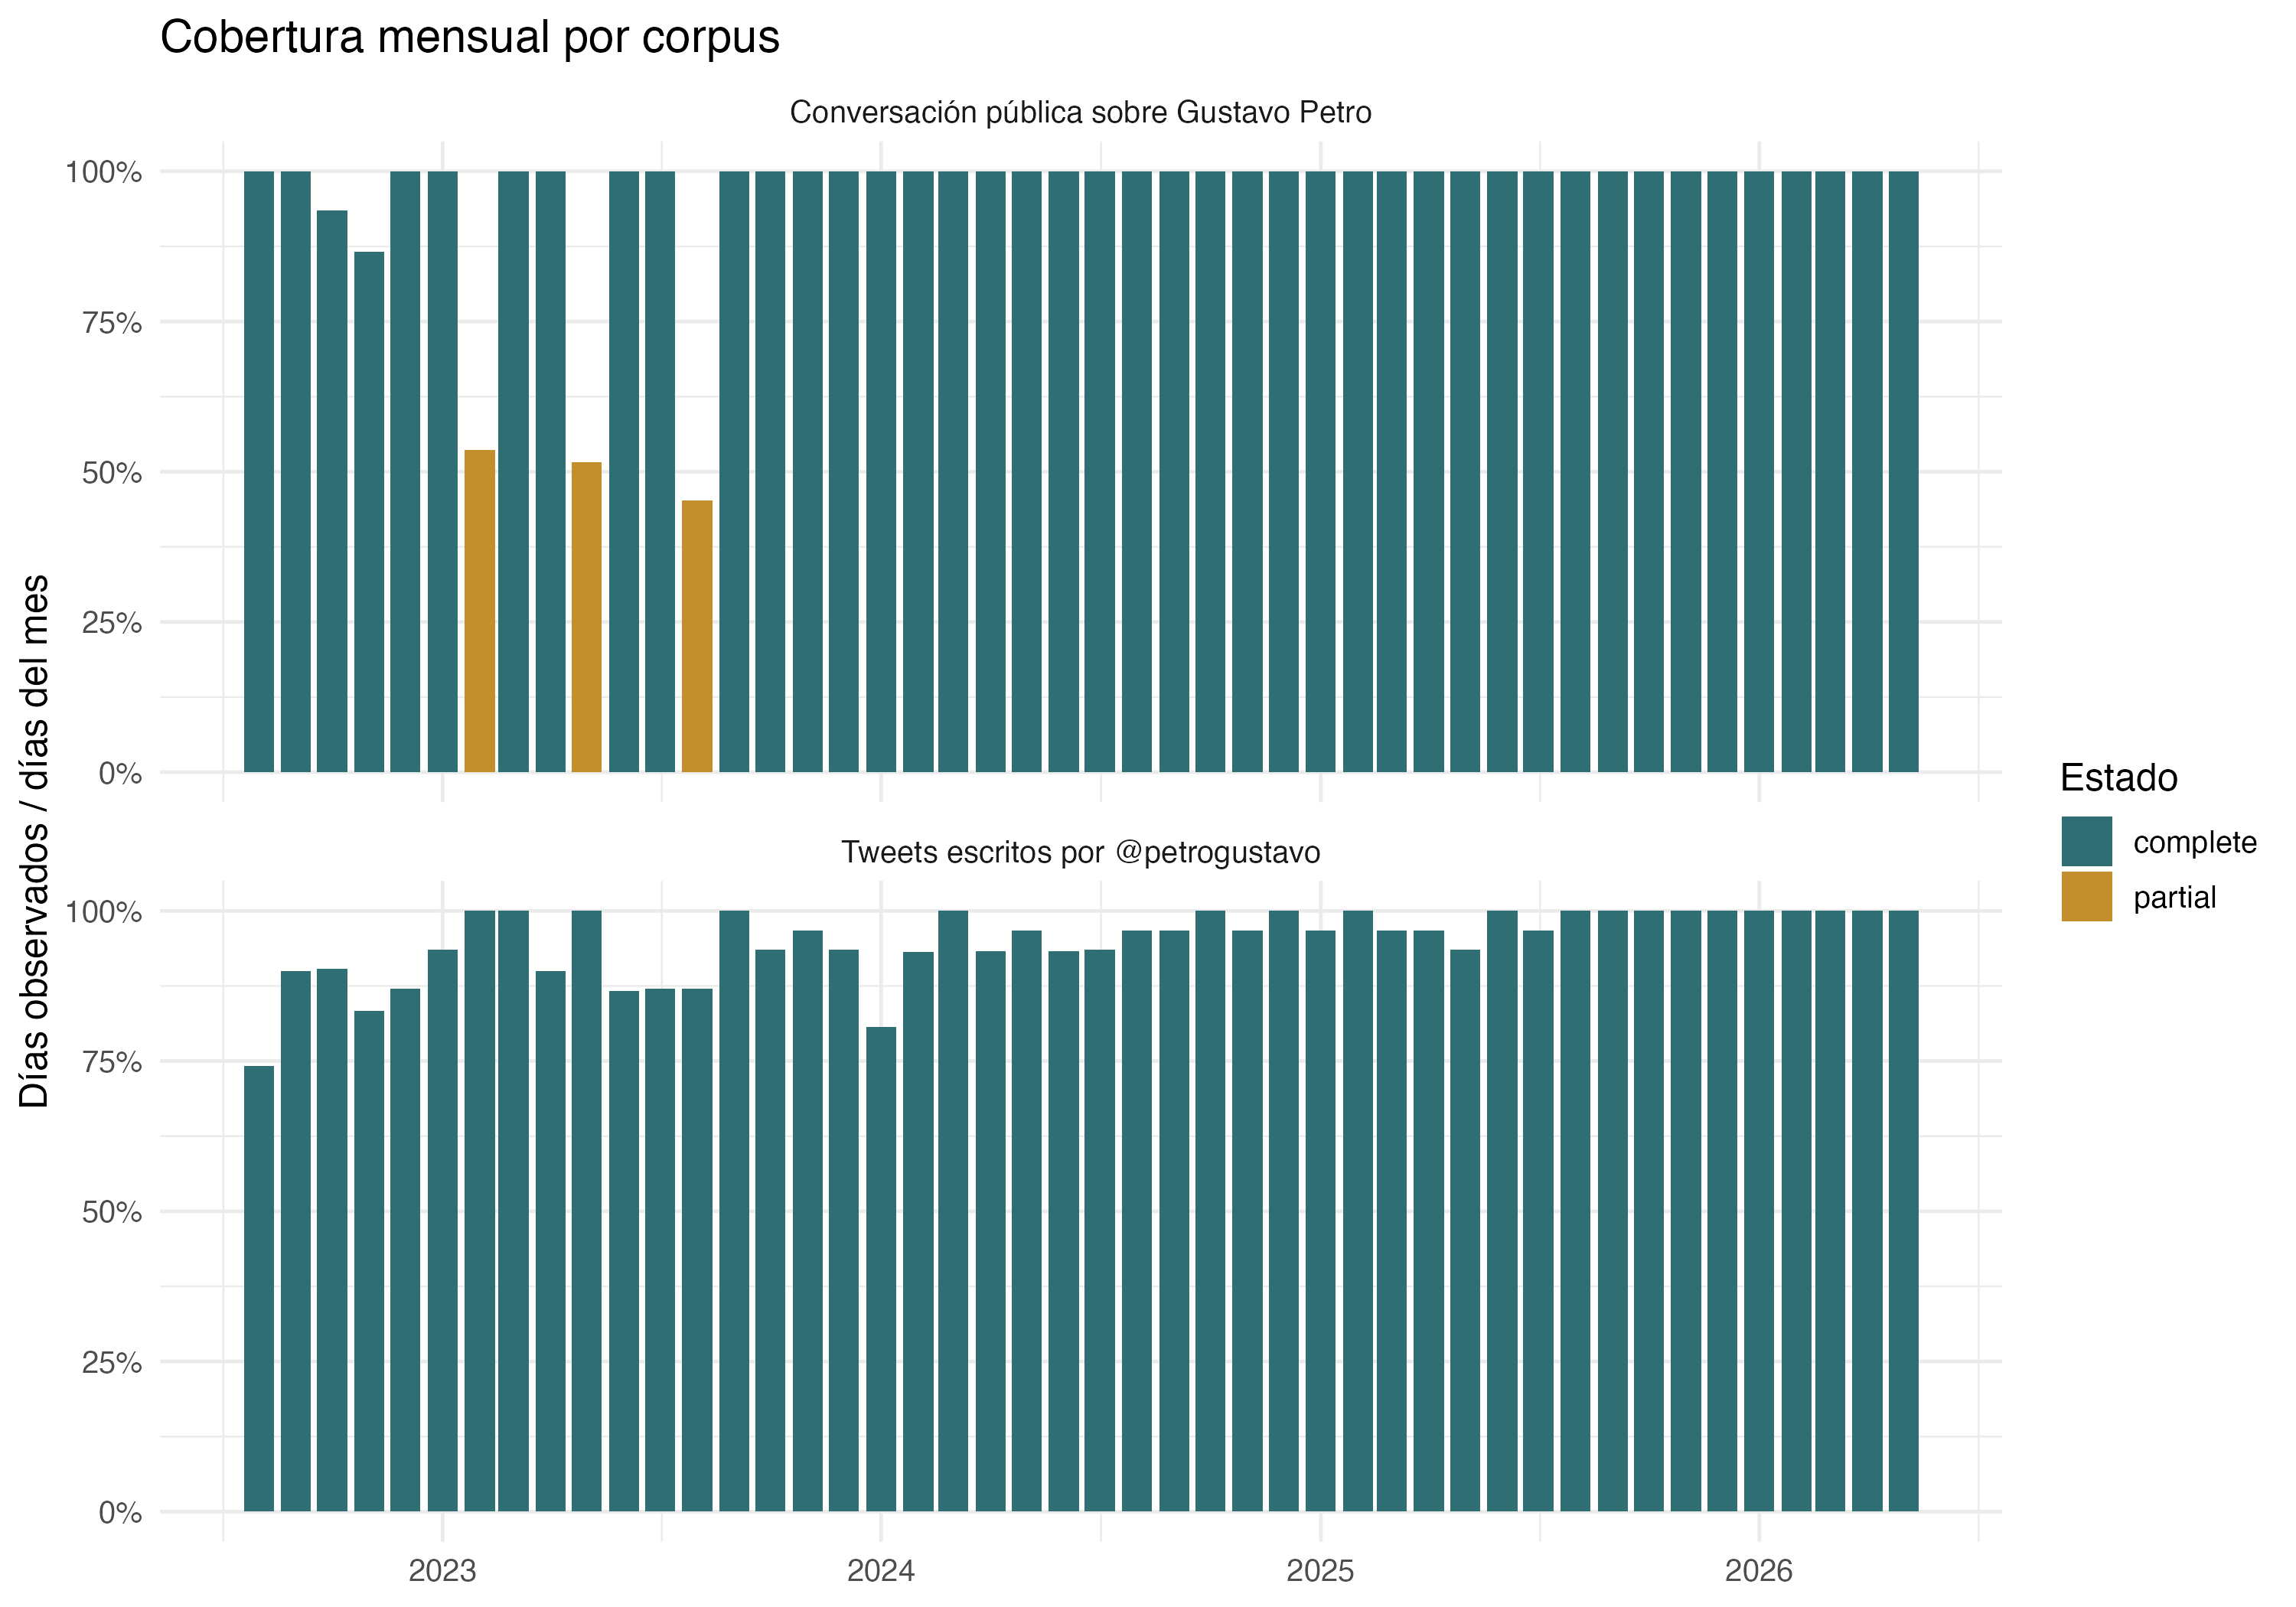
\includegraphics[width=0.9\linewidth,height=\textheight,keepaspectratio]{figures/comparacion_corpus_cobertura.png}

}

\caption{\label{fig-coverage}Auditoría mensual de cobertura por corpus.}

\end{figure}%

\section{Sentimientos y emociones en contextos
políticos}\label{sentimientos-y-emociones-en-contextos-poluxedticos}

Los estudios económicos suelen enfatizar indicadores cuantitativos, como
producción, precios, tasas de interés o índices bursátiles. Sin embargo,
el análisis cualitativo y textual permite observar dimensiones de
expectativa, emoción y percepción que no aparecen directamente en las
series financieras (Pérez Llorente 2020). El análisis de sentimientos
convierte grandes volúmenes de texto en medidas interpretables de tono,
polaridad y emoción (Medhat, Hassan, and Korashy 2014). En este
documento, el sentimiento no sustituye a los datos de mercado; funciona
como una señal discursiva que puede preceder, acompañar o seguir
movimientos financieros.

La relación entre emoción y decisión económica se apoya en la economía
del comportamiento. La idea de agentes plenamente racionales ha sido
cuestionada por teorías que muestran sesgos, exceso de confianza,
disonancia cognitiva, aversión a pérdidas y dependencia del punto de
referencia (Mullainathan and Thaler 2000; Kahneman 1979). Esta intuición
dialoga con la tradición de sentimientos morales de Adam Smith, donde
las decisiones sociales y económicas también dependen de simpatía,
juicio moral y reconocimiento social (Smith 1759). En mercados
financieros, el discurso presidencial puede importar porque las
expectativas son informativas y emocionales a la vez.

El paper original utilizó la rueda de emociones de Plutchik para
interpretar alegría, tristeza, ira, miedo, sorpresa, aversión, confianza
y anticipación (Plutchik 2003). El análisis de sentimientos en contextos
políticos latinoamericanos también ha usado diccionarios, lexicones y
modelos supervisados/no supervisados para estudiar opinión pública,
marketing político y comunicación gubernamental (Romero Moreno et al.
2020; Gómez-Torres et al. 2018; Cornejo 2022). La versión actual
conserva el enfoque NRC/Plutchik mediante \texttt{syuzhet} (Jockers
2017) y el léxico de Mohammad y Turney (S. Mohammad and Turney 2010; S.
M. Mohammad and Turney 2013), y lo complementa con agregación diaria y
medidas temáticas mediante \texttt{sentometrics} (Ardia et al. 2021).

Twitter/X es especialmente útil para investigación política porque
hashtags, menciones y redes muestran cómo se organizan conversaciones,
apoyos, oposiciones y movilizaciones. Las guías de ciencia de datos
políticos en R han destacado su utilidad para análisis reproducible
(Urdinez and Cruz 2020), mientras que la literatura sobre hashtags
muestra su papel en acción conectiva, feminismo digital y activismo
racial (Trott 2018; Ince, Rojas, and Davis 2017). En este documento, las
etiquetas y menciones permiten identificar quién participa en la
conversación sobre Petro y qué temas concentran polarización.

\begin{figure}

\centering{

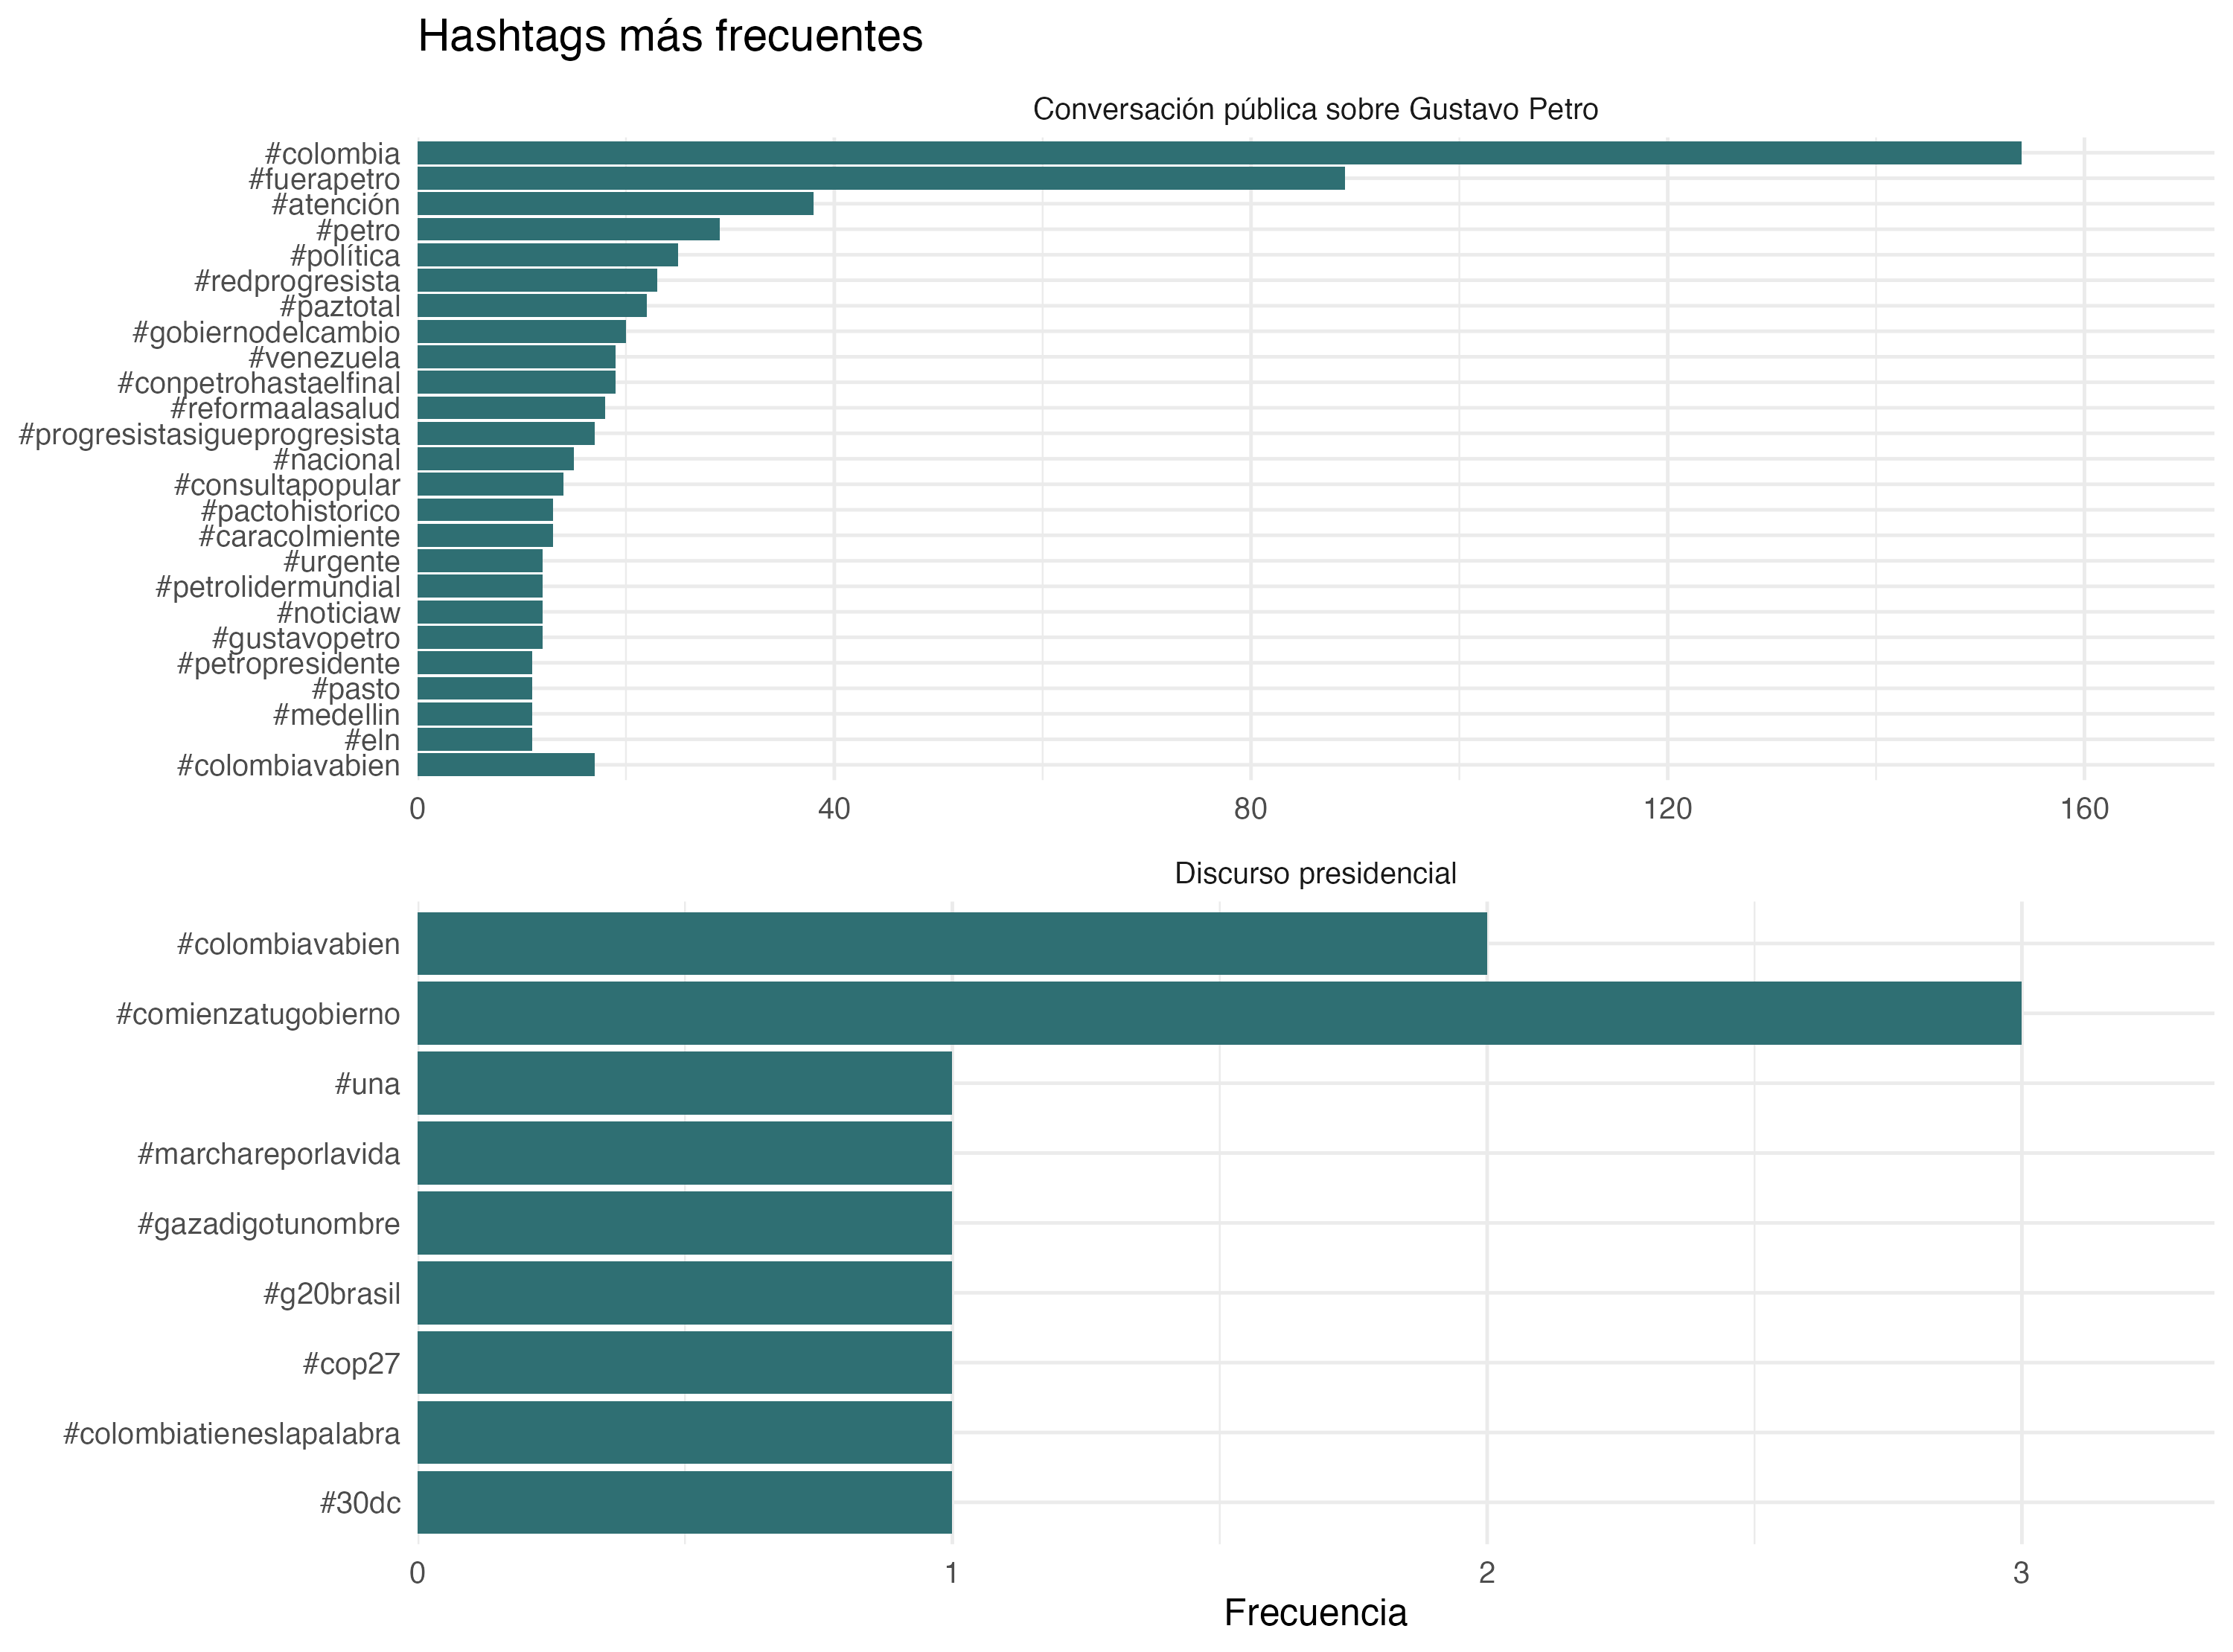
\includegraphics[width=0.8\linewidth,height=\textheight,keepaspectratio]{figures/hashtags_principales.png}

}

\caption{\label{fig-hashtags}Hashtags asociados a Gustavo Petro en el
corpus actualizado.}

\end{figure}%

\begin{figure}

\centering{

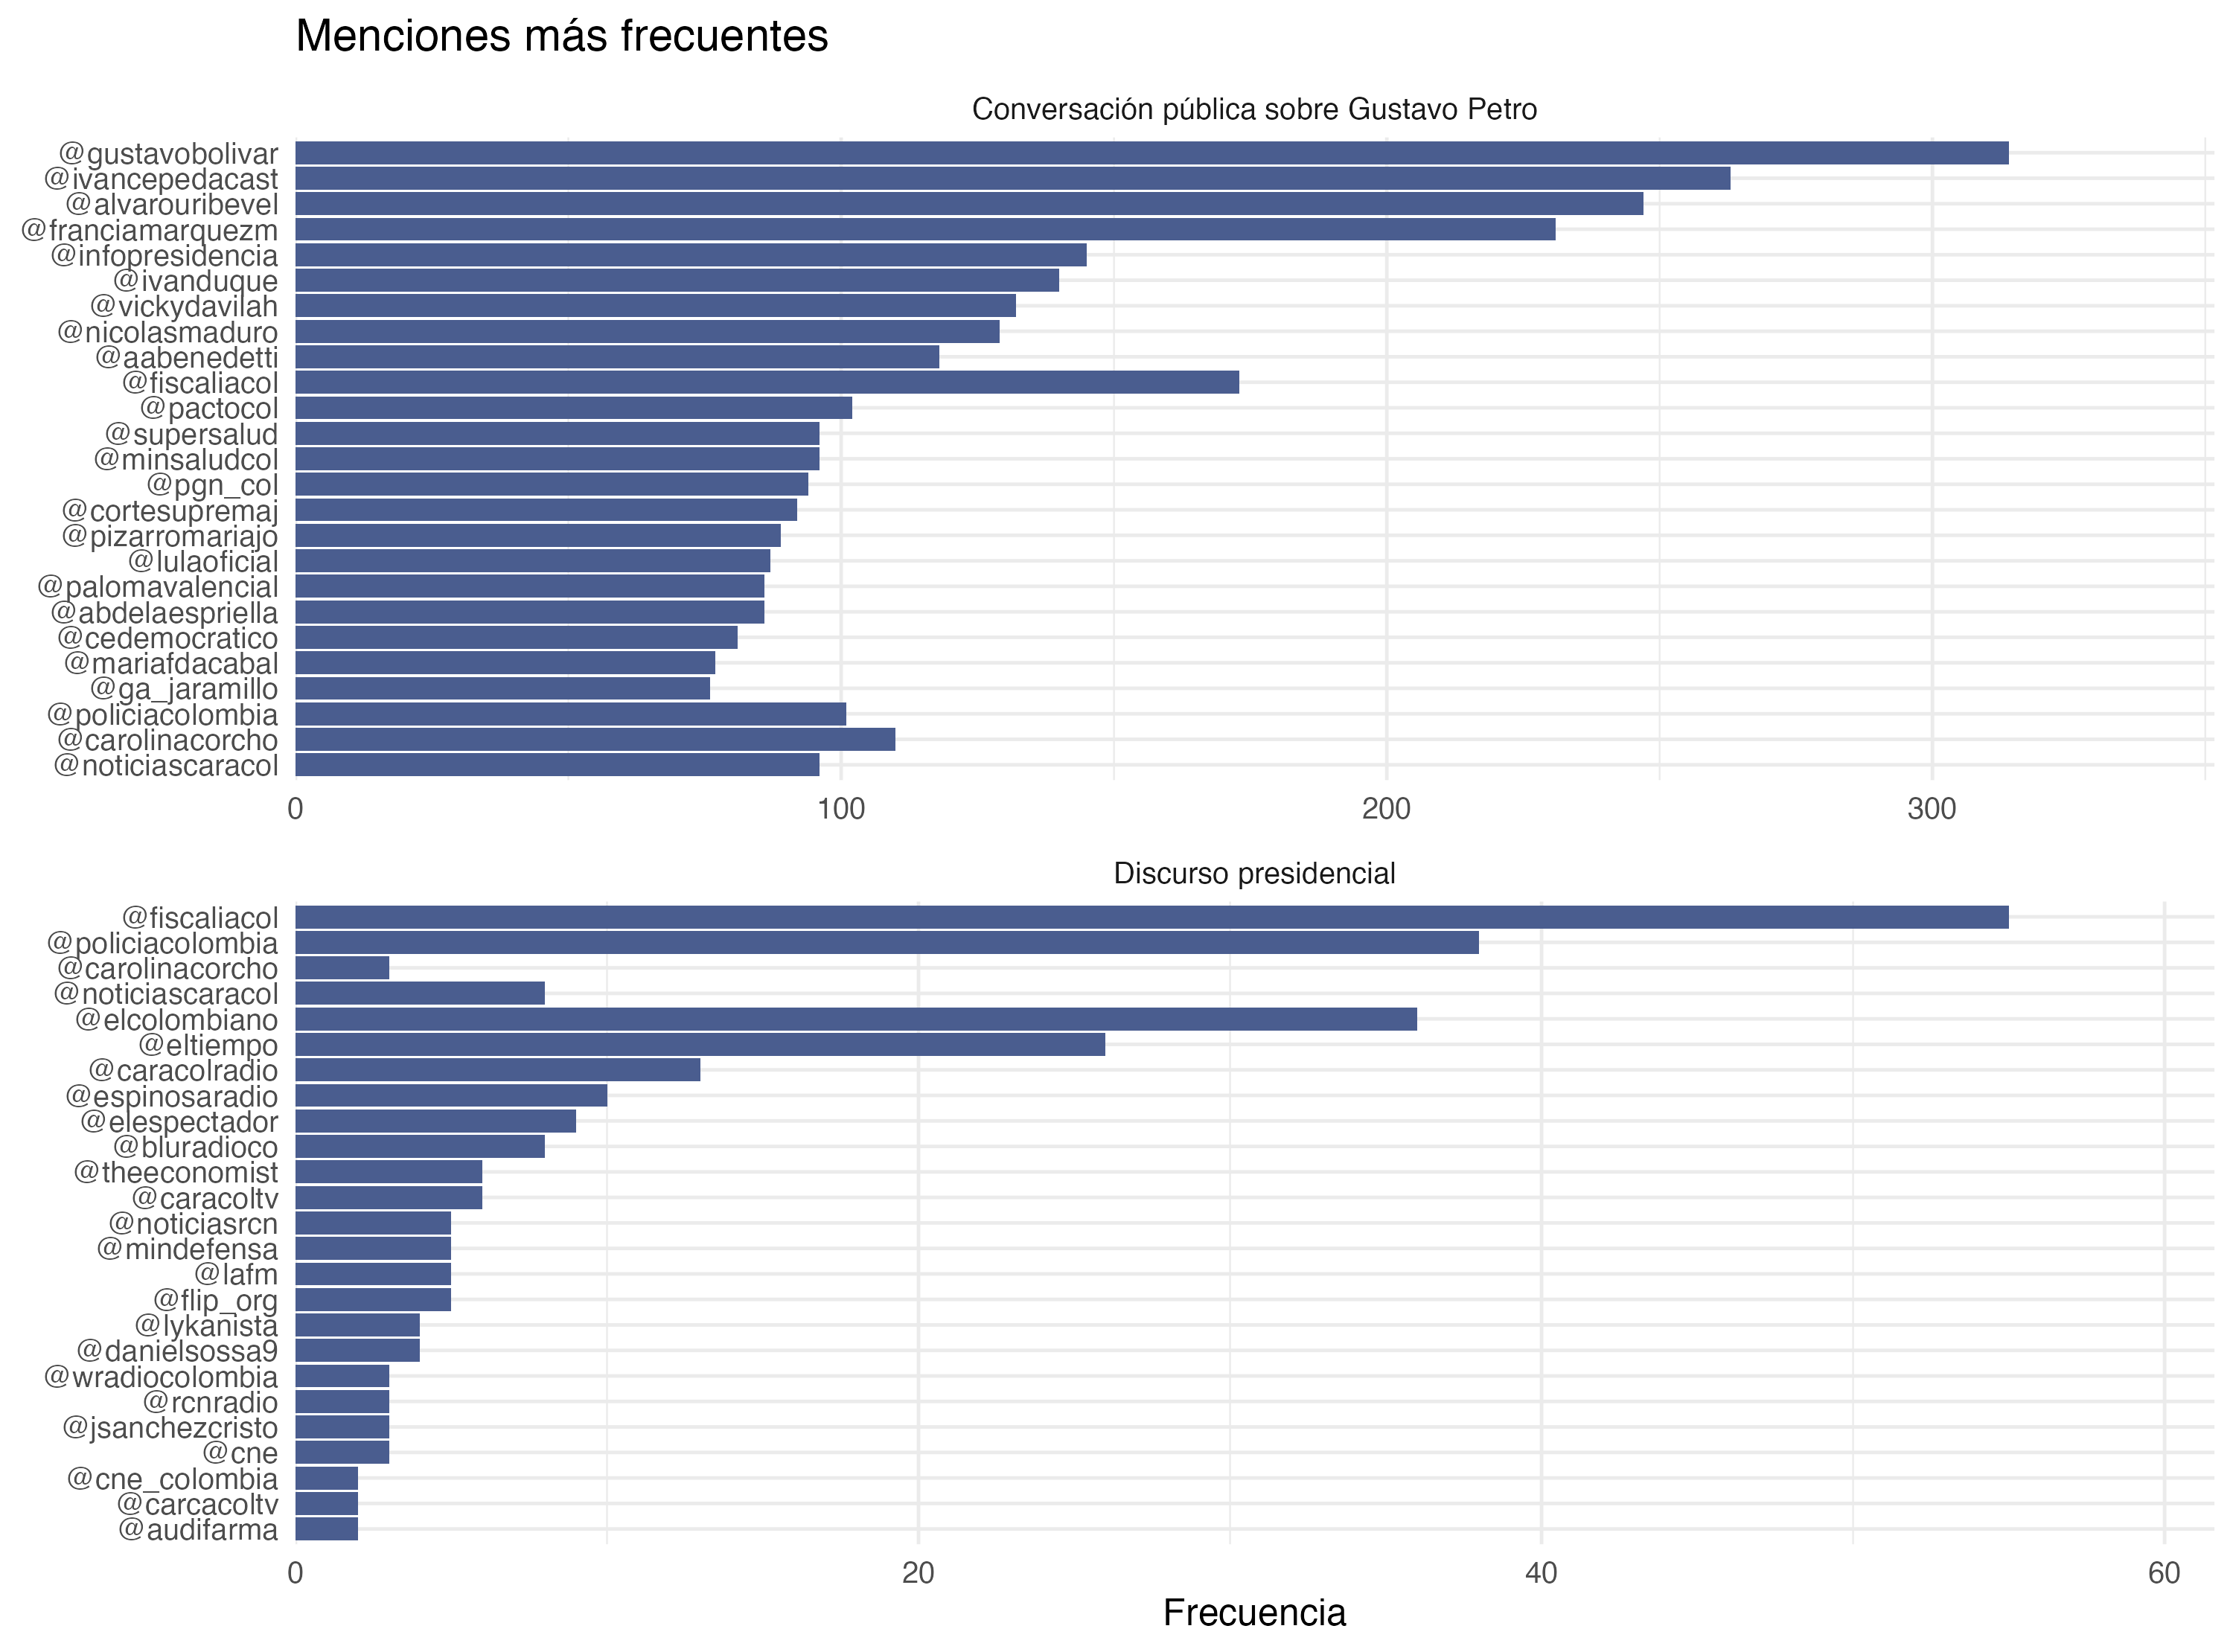
\includegraphics[width=0.8\linewidth,height=\textheight,keepaspectratio]{figures/menciones_principales.png}

}

\caption{\label{fig-mentions}Principales menciones dentro del corpus
asociado a Petro.}

\end{figure}%

\section{Metodología}\label{metodologuxeda}

El documento original realizó una caracterización semántica y
sentimental de microblogs de Twitter junto con información histórica de
mercado. Esta versión conserva esa arquitectura y la vuelve reproducible
mediante dos contratos estables: \texttt{tweets\_master.csv}, con una
fila por tweet y clave \texttt{(corpus,\ id)}, y
\texttt{market\_master.csv}, con una fila por fecha. El script prepara
datos determinísticos; el cuaderno reconstruye la clasificación temática
y conserva las decisiones NLP, sentimiento, IPI, redes y econometría.
Esta separación permite comparar emisor y conversación pública sin
mezclar corpus ni perder trazabilidad.

El primer paso consiste en recolección, auditoría y normalización. El
scraping histórico se relaciona con flujos de trabajo de la API de
Twitter y herramientas como \texttt{rtweet} (Kearney 2019). La
literatura reciente advierte que Twitter como dato exige documentar
costos, restricciones, cambios de API y sesgos de cobertura
(Steinert-Threlkeld 2018; K. Chen, Duan, and Yang 2022). La versión
original también usó inferencia de género desde nombres en español
mediante \texttt{genero} (Marin Diaz 2020); la actualización prioriza
texto, temas y mercado porque la agregación diaria es más robusta para
unir discurso con series financieras.

El segundo paso es la construcción del corpus. El texto se limpia,
tokeniza y transforma en matrices documento-característica con
\texttt{quanteda} (Benoit, Nulty, et al. 2018; Benoit, Watanabe, et al.
2018). La minería textual práctica en R, el enfoque tidy text y la
estadística de keyness permiten extraer términos distintivos y
relaciones semánticas entre documentos (Kwartler 2017; Silge and
Robinson 2017; Bondi and Scott 2010). El análisis de coocurrencias,
colocaciones y collexemas sigue la tradición de relaciones léxicas entre
palabras, construcciones y contextos (Schweinberger 2023; Wiedemann and
Niekler 2017; Stefanowitsch and Gries 2003, 2005).

El tercer paso caracteriza la estructura semántica. La versión original
usaba redes de conexiones, coocurrencias, dendrogramas y análisis
multivariante. Esta actualización conserva esa lógica: la clasificación
jerárquica de Ward ayuda a visualizar similitudes entre términos
(El-Hamdouchi and Willett 1986), los biplots y análisis multivariantes
apoyan la lectura de proximidades semánticas (Field, Miles, and Field
2012; Husson, Lê, and Pagès 2016), y las redes discursivas muestran
asociaciones entre etiquetas, cuentas y términos. En las redes, los
nodos representan cuentas o términos; las conexiones representan
co-menciones o coocurrencias dentro de una ventana textual, los pesos
cuentan la recurrencia de esas asociaciones y las comunidades agrupan
nodos con mayor densidad interna (Kolaczyk and Csárdi 2020). Para
hashtags y menciones se adopta el estilo visual del ejemplo oficial de
análisis de Twitter de \texttt{quanteda}: etiquetas visibles, nodos
oscuros, aristas curvas y grosor proporcional a la frecuencia de
coaparición (quanteda team 2026). Wordfish estima posiciones textuales a
partir de patrones de uso de palabras (Slapin and Proksch 2008).

El cuarto paso modela temas y lenguaje. Los modelos de tópicos permiten
resumir corpus de alta dimensión (D. M. Blei, Ng, and Jordan 2003; D.
Blei 2009), y el modelo estructural de tópicos agrega covariables y
diagnósticos de coherencia/exclusividad (Roberts, Stewart, and Tingley
2019). La actualización incorpora además una clasificación temática con
supervisión débil: se entrenan etiquetas derivadas de reglas no
\texttt{otros}, se evalúan contra un modelo base con partición holdout y
sólo se reasignan textos de \texttt{otros} cuando la confianza es
conservadora. Esta estrategia sigue la lógica de evaluación supervisada
de texto, pero se presenta como análisis de sensibilidad, no como
reemplazo de etiquetas humanas (Hvitfeldt and Silge 2022). La
actualización incorpora \texttt{spacyr} para enriquecer el corpus con
entidades, lemas y patrones sintácticos (Benoit and Matsuo 2023). Esta
capa es útil para paz total, porque permite identificar actores,
instituciones, territorios y términos de negociación que no siempre
aparecen como palabras clave aisladas (Hirschberg and Manning 2015).

El quinto paso une sentimientos y mercado. La polaridad, el volumen y el
Índice de Presión Informacional se calculan por día y por corpus, y
\texttt{sentometrics} agrega señales por tema y lexicón (Misuraca et al.
2020; Ardia et al. 2021). La literatura de opinion mining financiero
motiva interpretar esos indicadores como señales textuales de
expectativa y tono, no como mecanismos causales por sí mismos (C.-C.
Chen, Huang, and Chen 2022; Kumar and Bhatia 2014). Las variables
financieras provienen de BanRep: TRM como tipo de cambio, COLCAP como
proxy accionario y TES cero cupón en pesos a 1, 5 y 10 años. La
pendiente TES 10Y-1Y se calcula como indicador de expectativas
soberanas. La evaluación econométrica usa pruebas de Granger por corpus
para TRM, COLCAP, TES 10Y y pendiente TES; VAR e impulsos-respuesta se
reportan solo si existen suficientes casos completos. La interpretación
temporal sigue referencias aplicadas de series y econometría en R
(Hyndman and Athanasopoulos 2018; Kleiber and Zeileis 2008).

\begin{figure}

\centering{

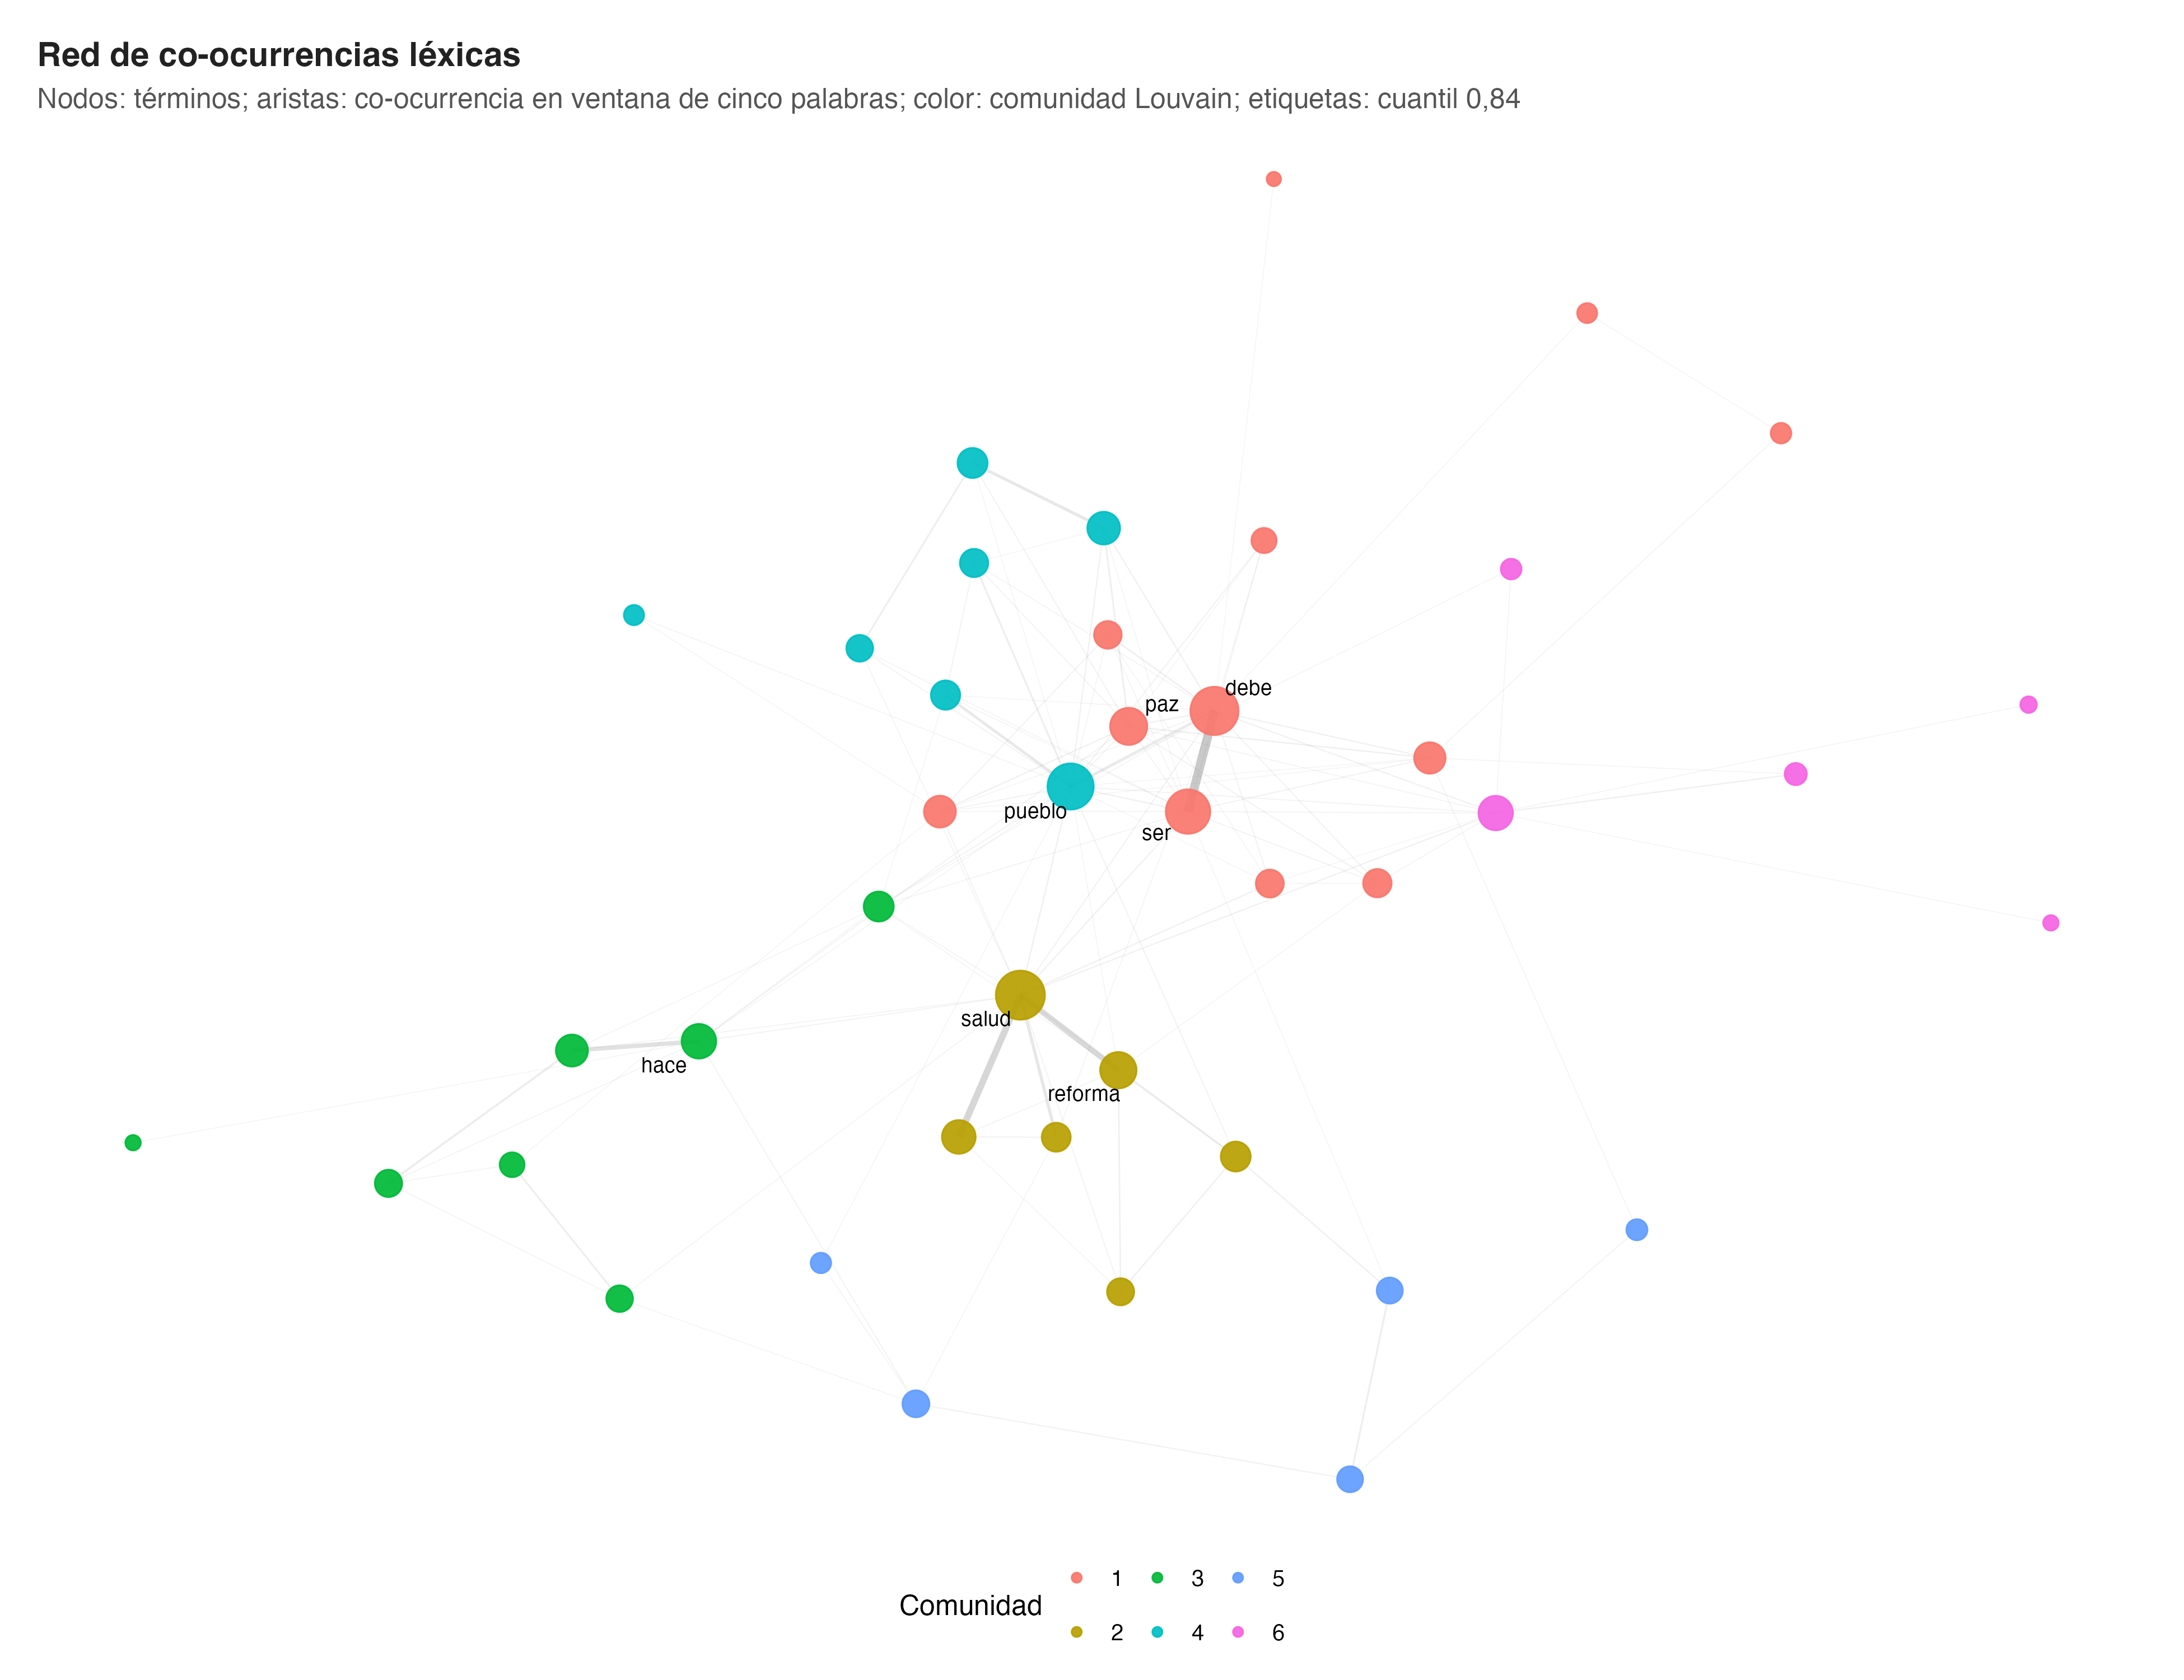
\includegraphics[width=0.8\linewidth,height=\textheight,keepaspectratio]{figures/red_coocurrencias_corpus.png}

}

\caption{\label{fig-cooc}Red de coocurrencias léxicas del corpus
actualizado.}

\end{figure}%

\begin{figure}

\centering{

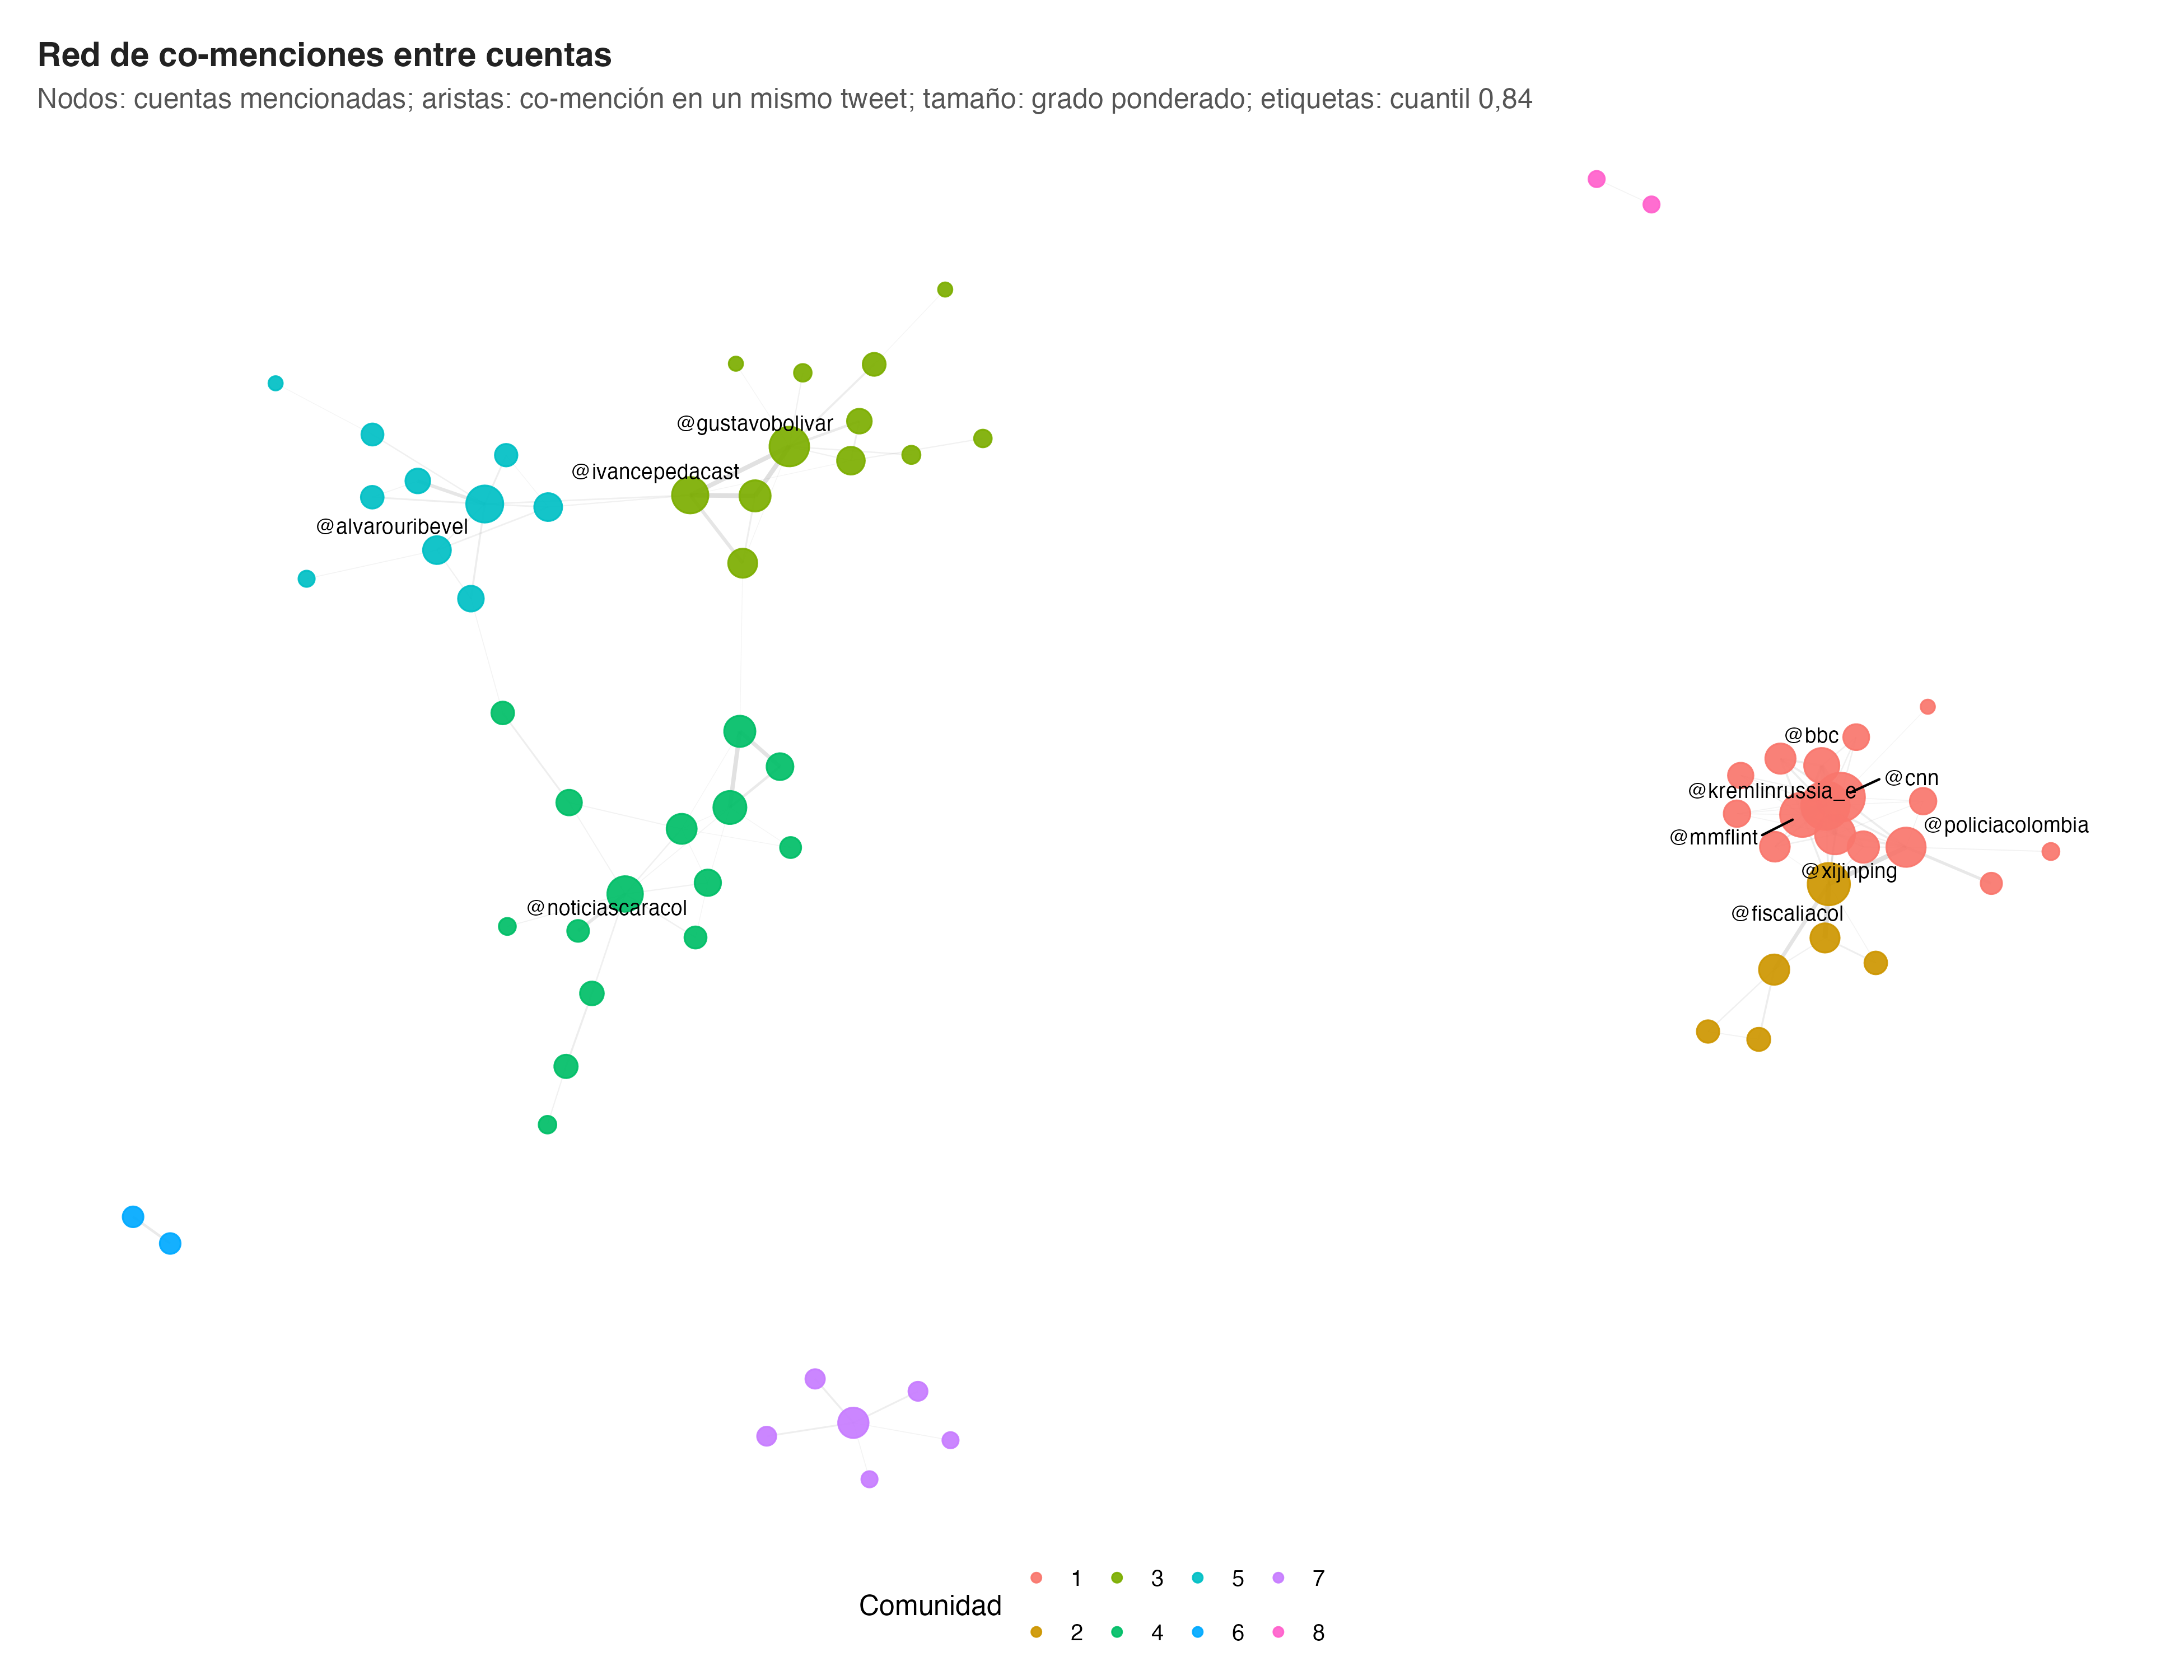
\includegraphics[width=0.8\linewidth,height=\textheight,keepaspectratio]{figures/red_menciones.png}

}

\caption{\label{fig-mentions-network}Red de co-menciones entre cuentas
del corpus actualizado.}

\end{figure}%

\begin{figure}

\centering{

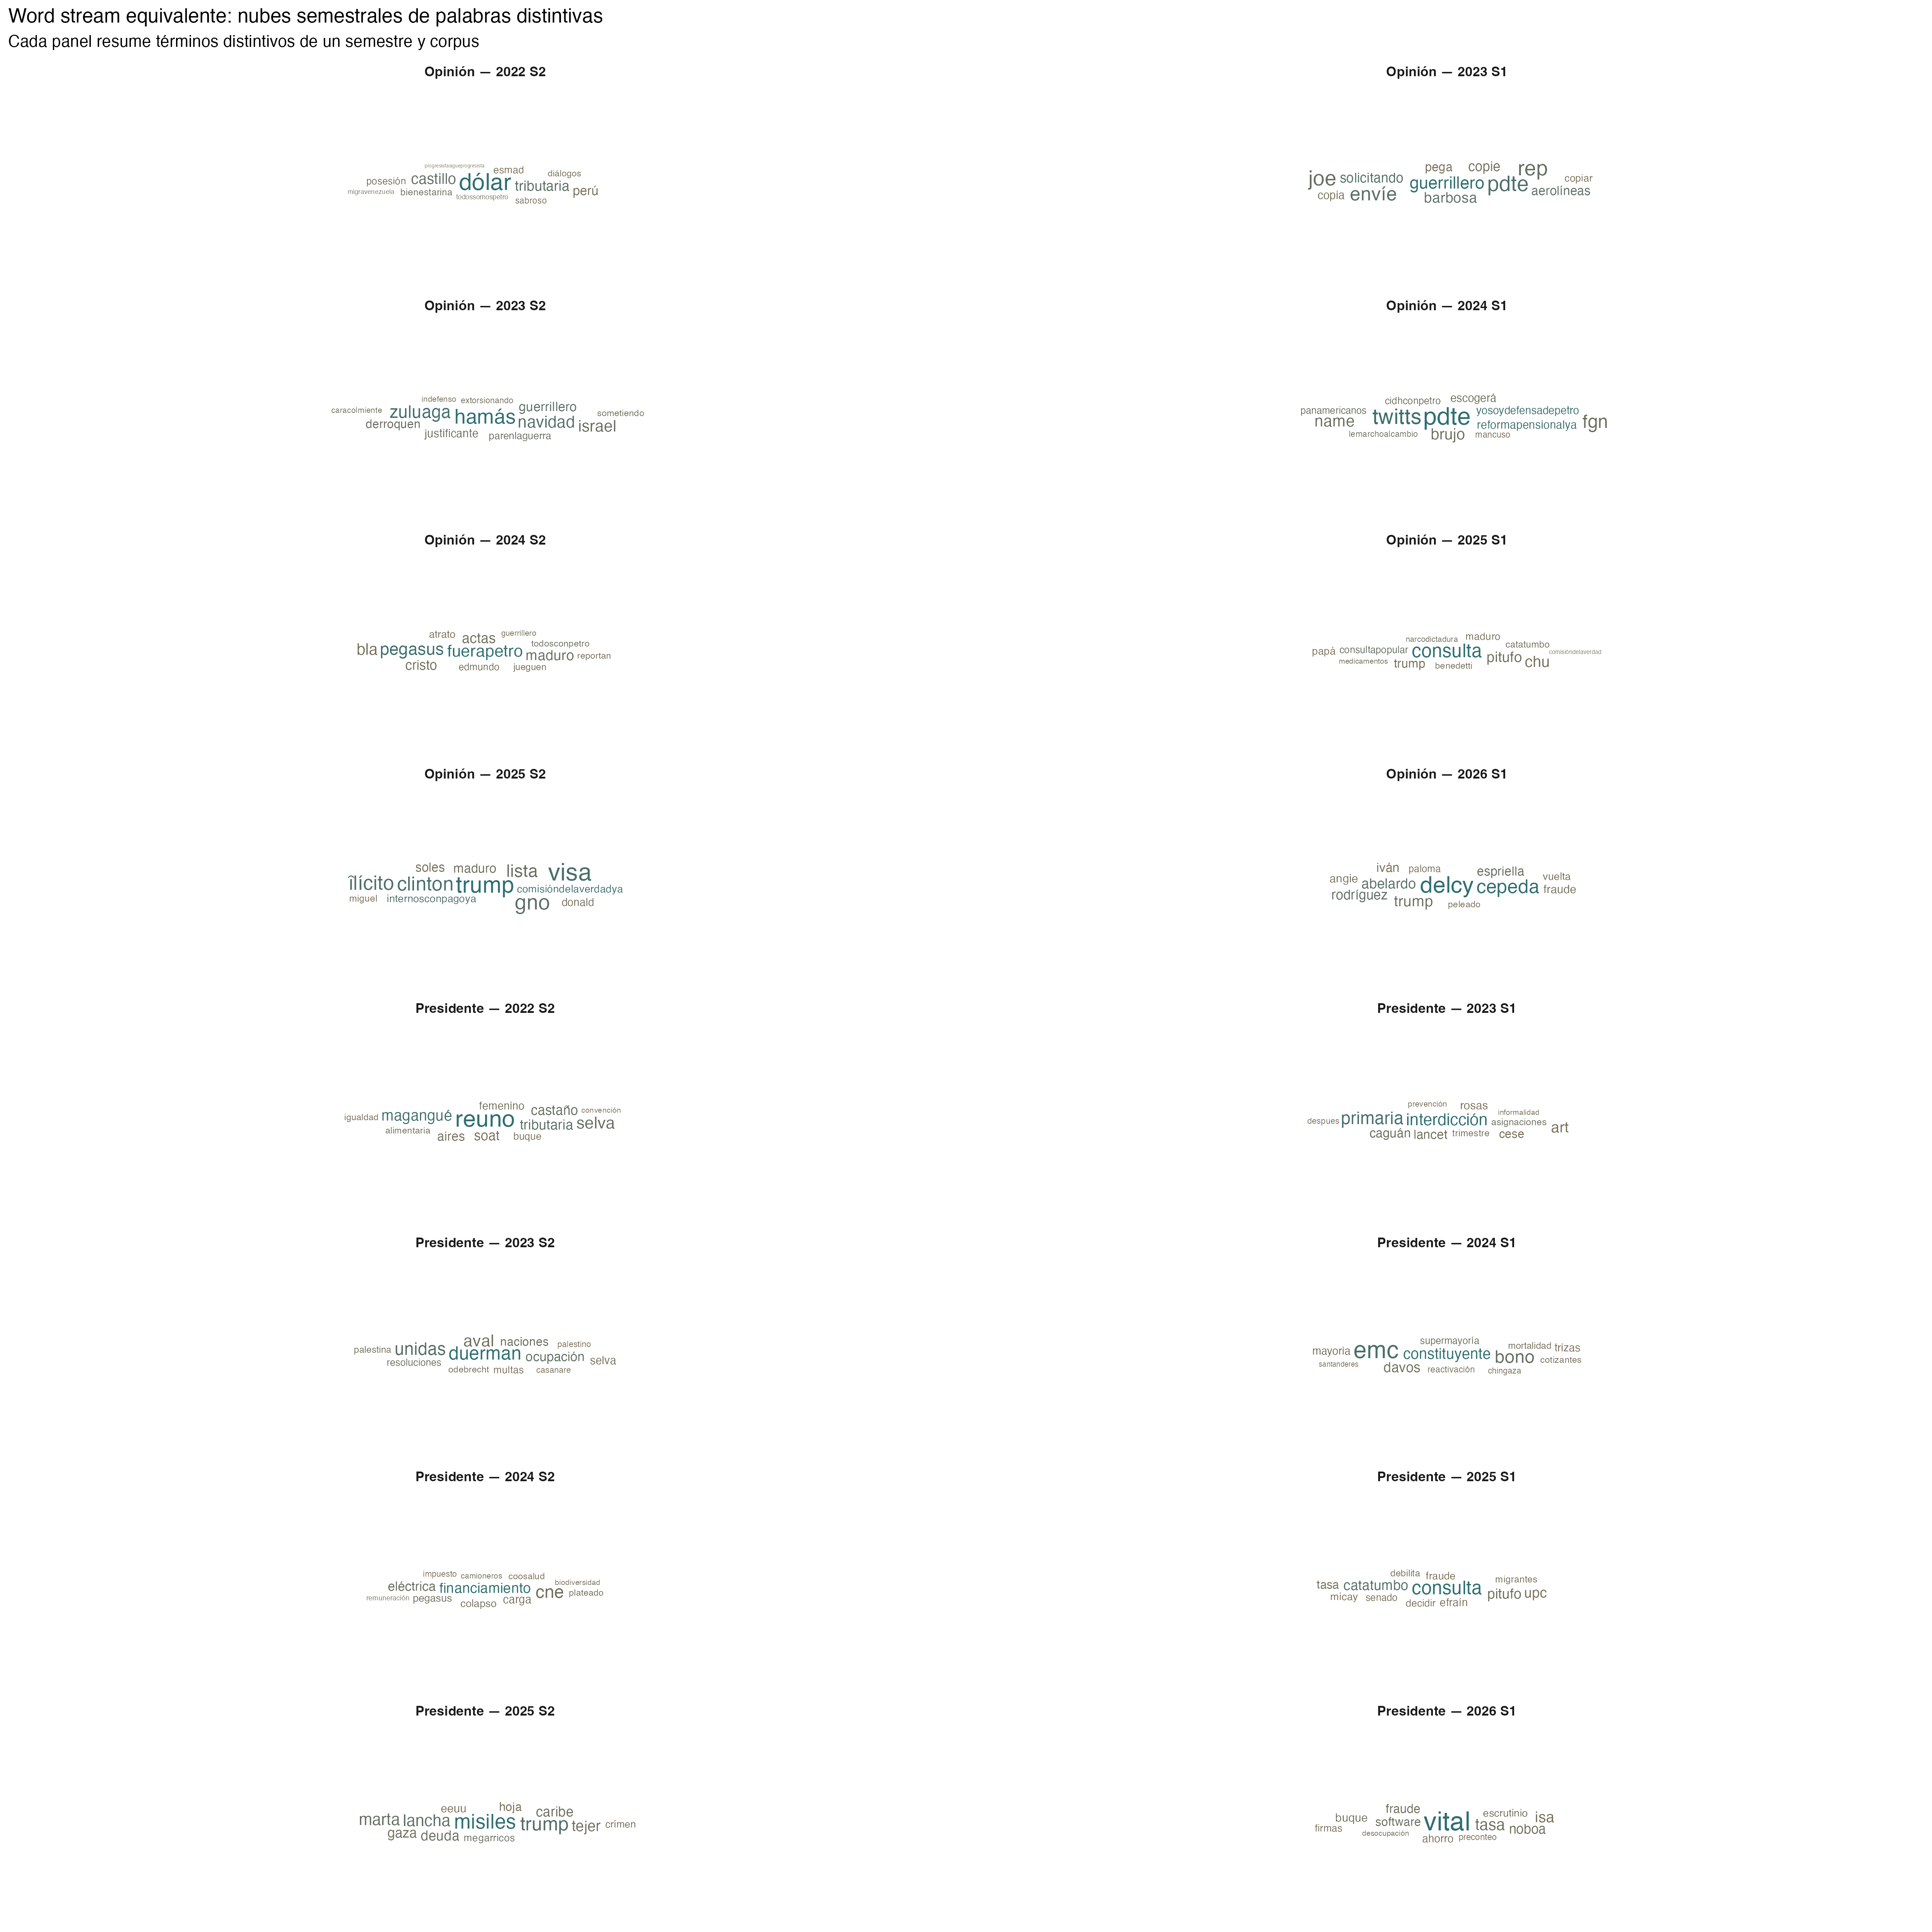
\includegraphics[width=0.9\linewidth,height=\textheight,keepaspectratio]{figures/wordcloud_temporal_periodos.png}

}

\caption{\label{fig-wordstream-cloud}Word stream equivalente: nubes
semestrales de palabras distintivas por corpus.}

\end{figure}%

\begin{figure}

\centering{

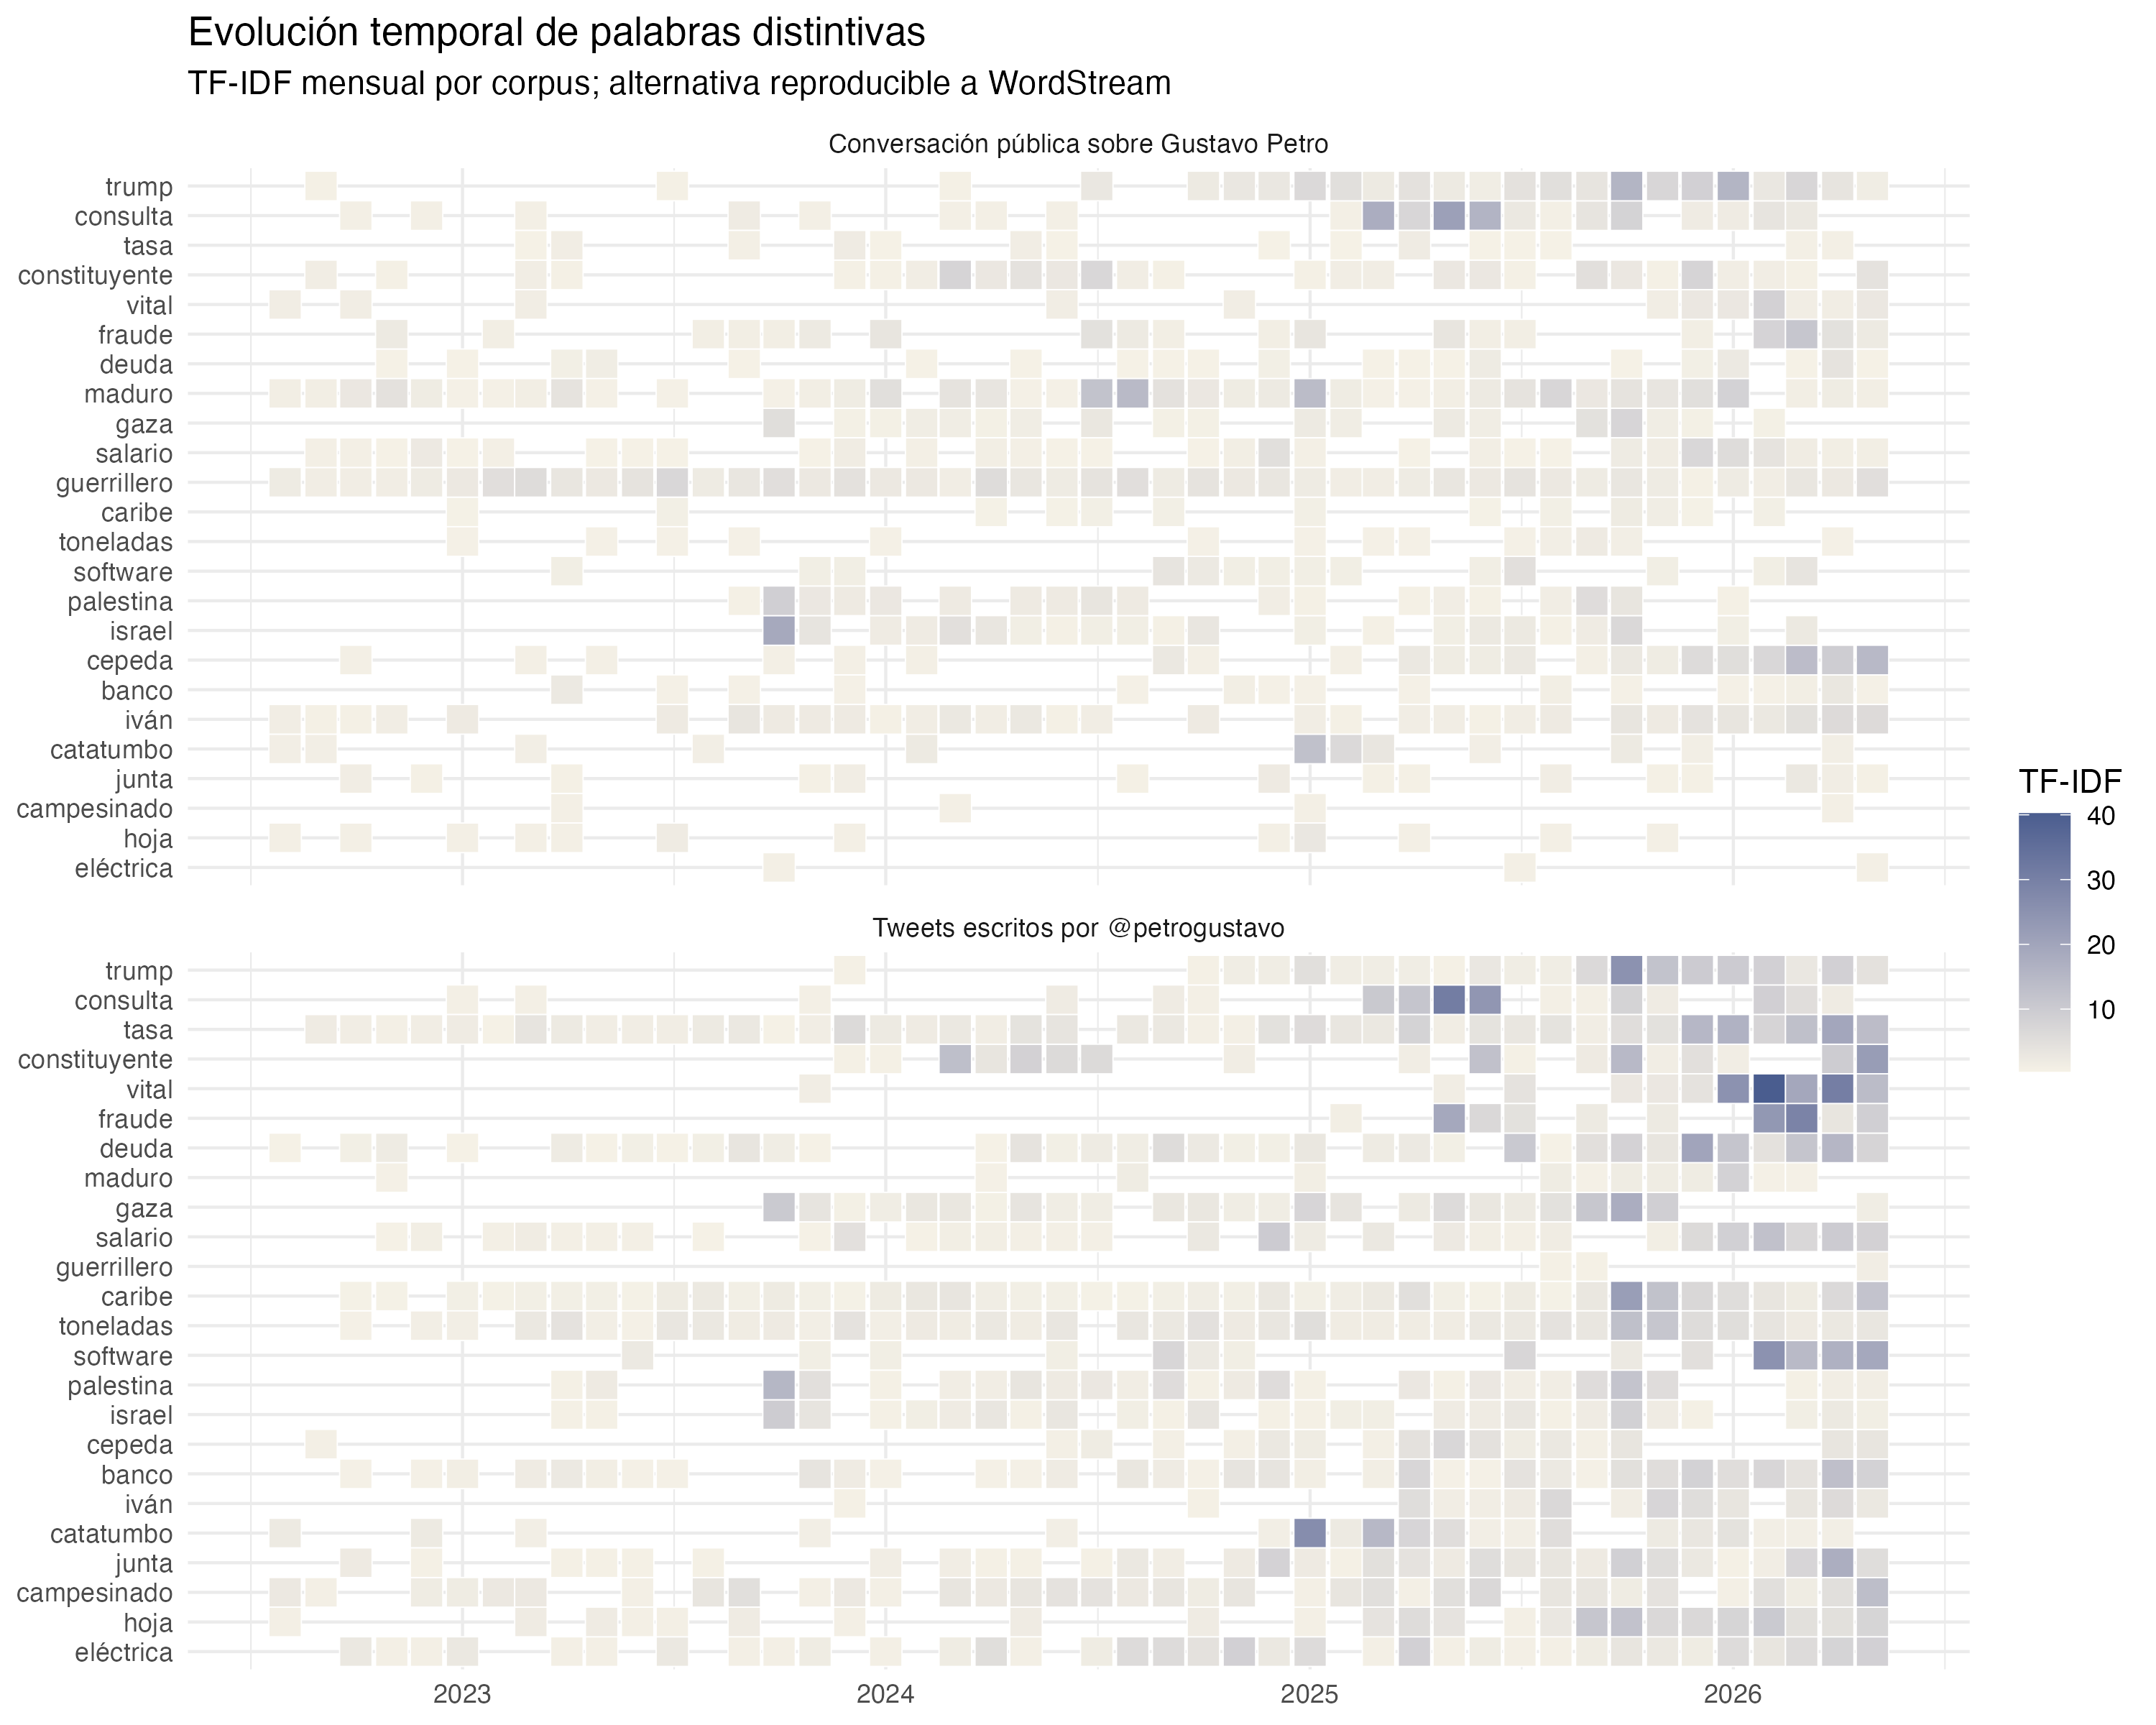
\includegraphics[width=0.9\linewidth,height=\textheight,keepaspectratio]{figures/wordstream_tfidf_temporal.png}

}

\caption{\label{fig-wordstream}Heatmap temporal TF-IDF de palabras por
mes y corpus.}

\end{figure}%

\begin{figure}

\centering{

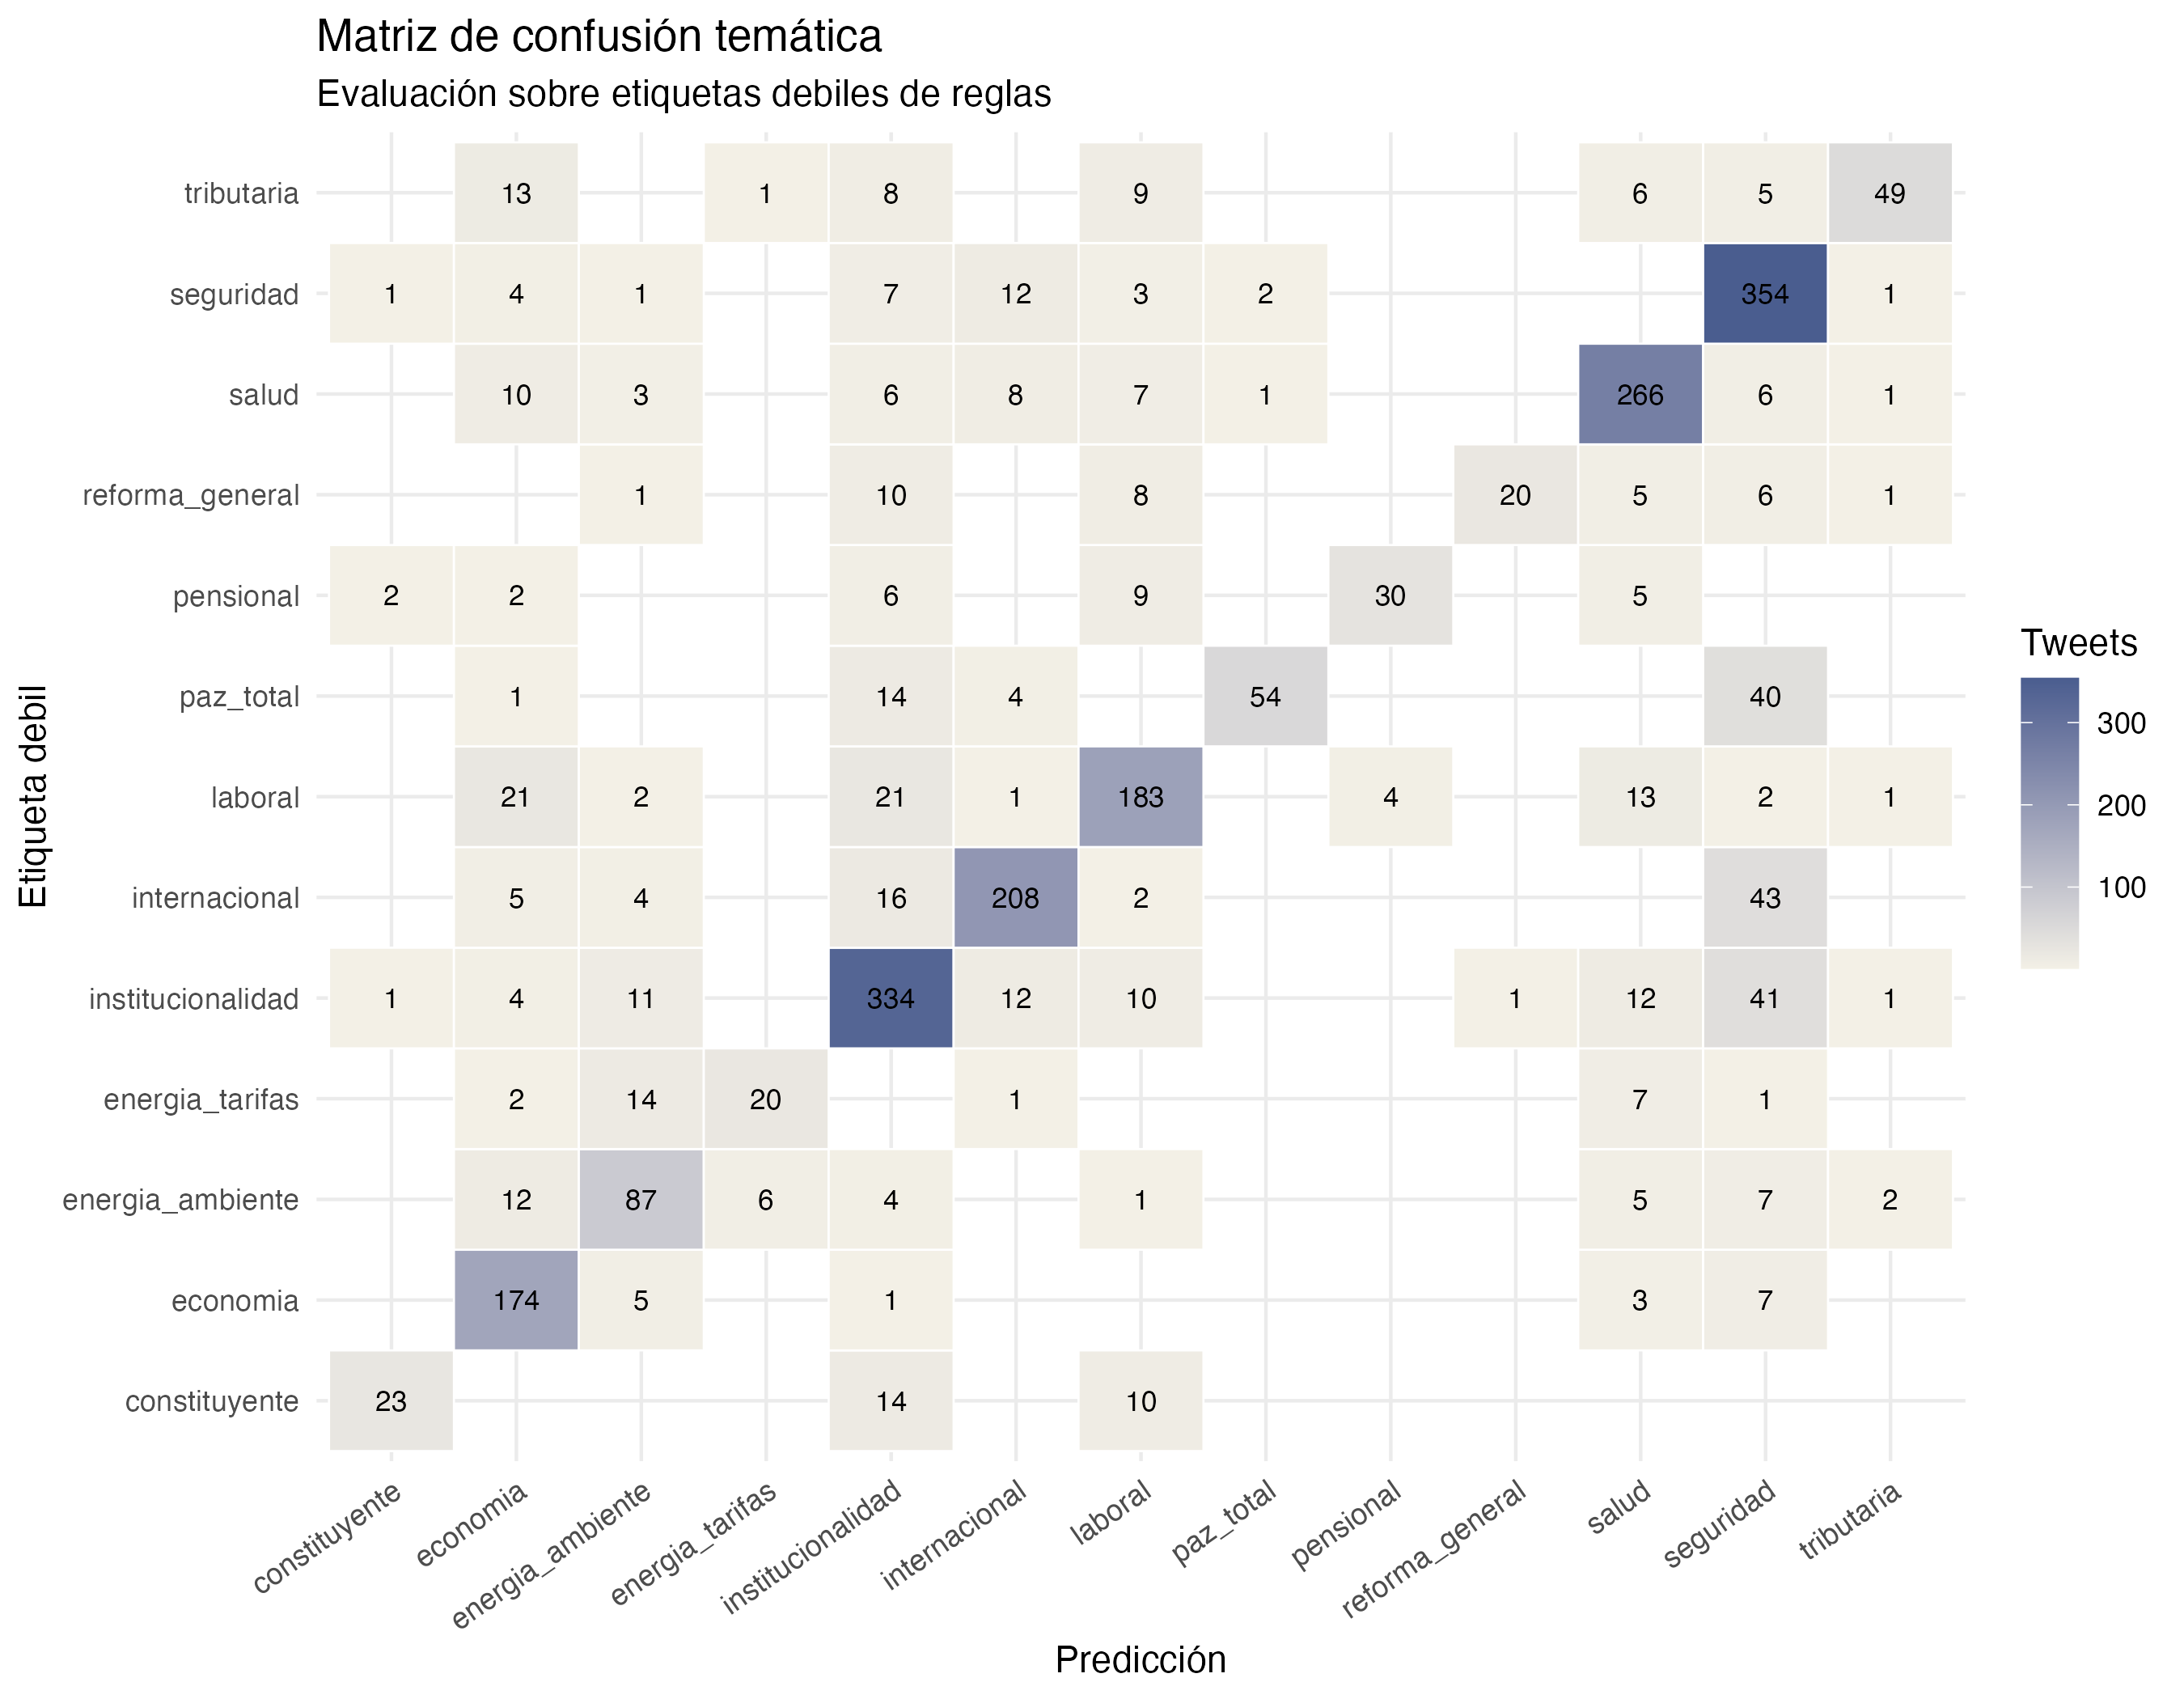
\includegraphics[width=0.8\linewidth,height=\textheight,keepaspectratio]{figures/ml_matriz_confusion_temas.png}

}

\caption{\label{fig-ml-confusion}Matriz de confusión del clasificador
temático con supervisión débil.}

\end{figure}%

\begin{figure}

\centering{

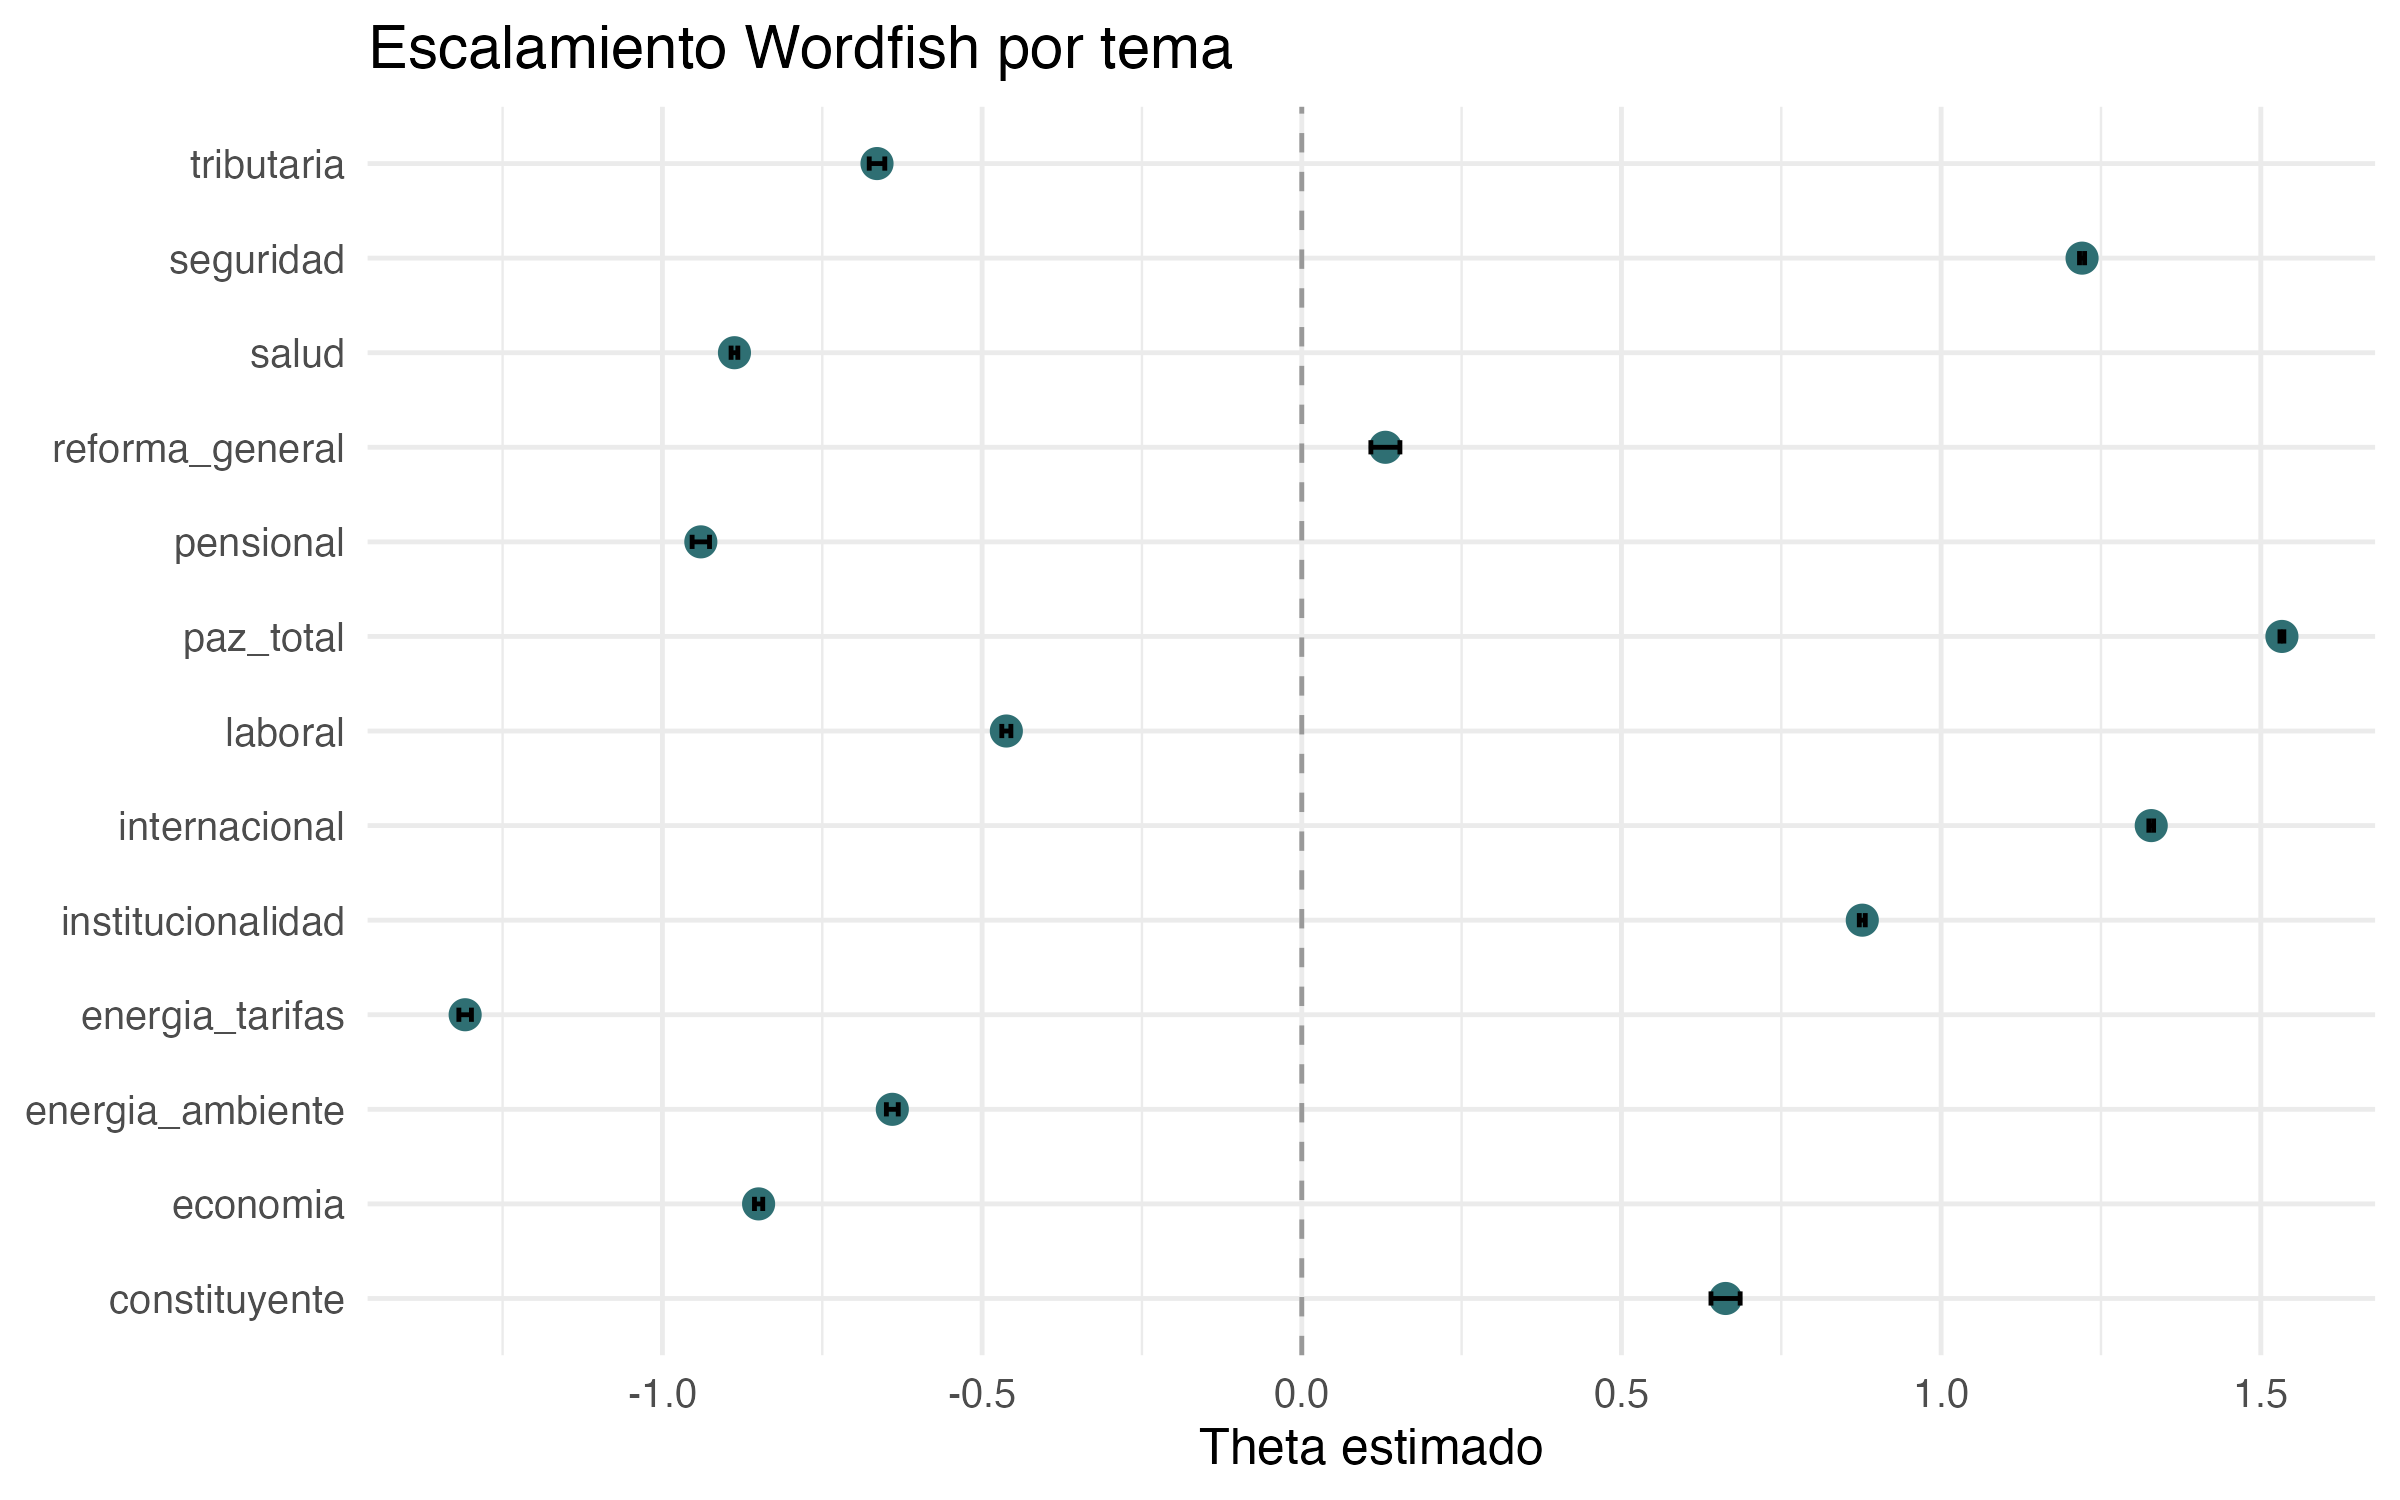
\includegraphics[width=0.8\linewidth,height=\textheight,keepaspectratio]{figures/wordfish_reformas.png}

}

\caption{\label{fig-wordfish}Escalamiento Wordfish por tema de reforma.}

\end{figure}%

\section{Resultados}\label{resultados}

La auditoría de datos confirma que el corpus \texttt{@Petro} amplía de
manera sustancial el ejercicio original de marzo-abril de 2023 y que los
tweets escritos por \texttt{@petrogustavo} permiten aislar el discurso
presidencial directo. La ventana disponible cubre agosto de 2022 a mayo
de 2026, con meses parciales marcados explícitamente. Esto permite
distinguir entre controversias sociales, mensajes presidenciales y
patrones repetidos de sentimiento y reacción financiera.

\begin{figure}

\centering{

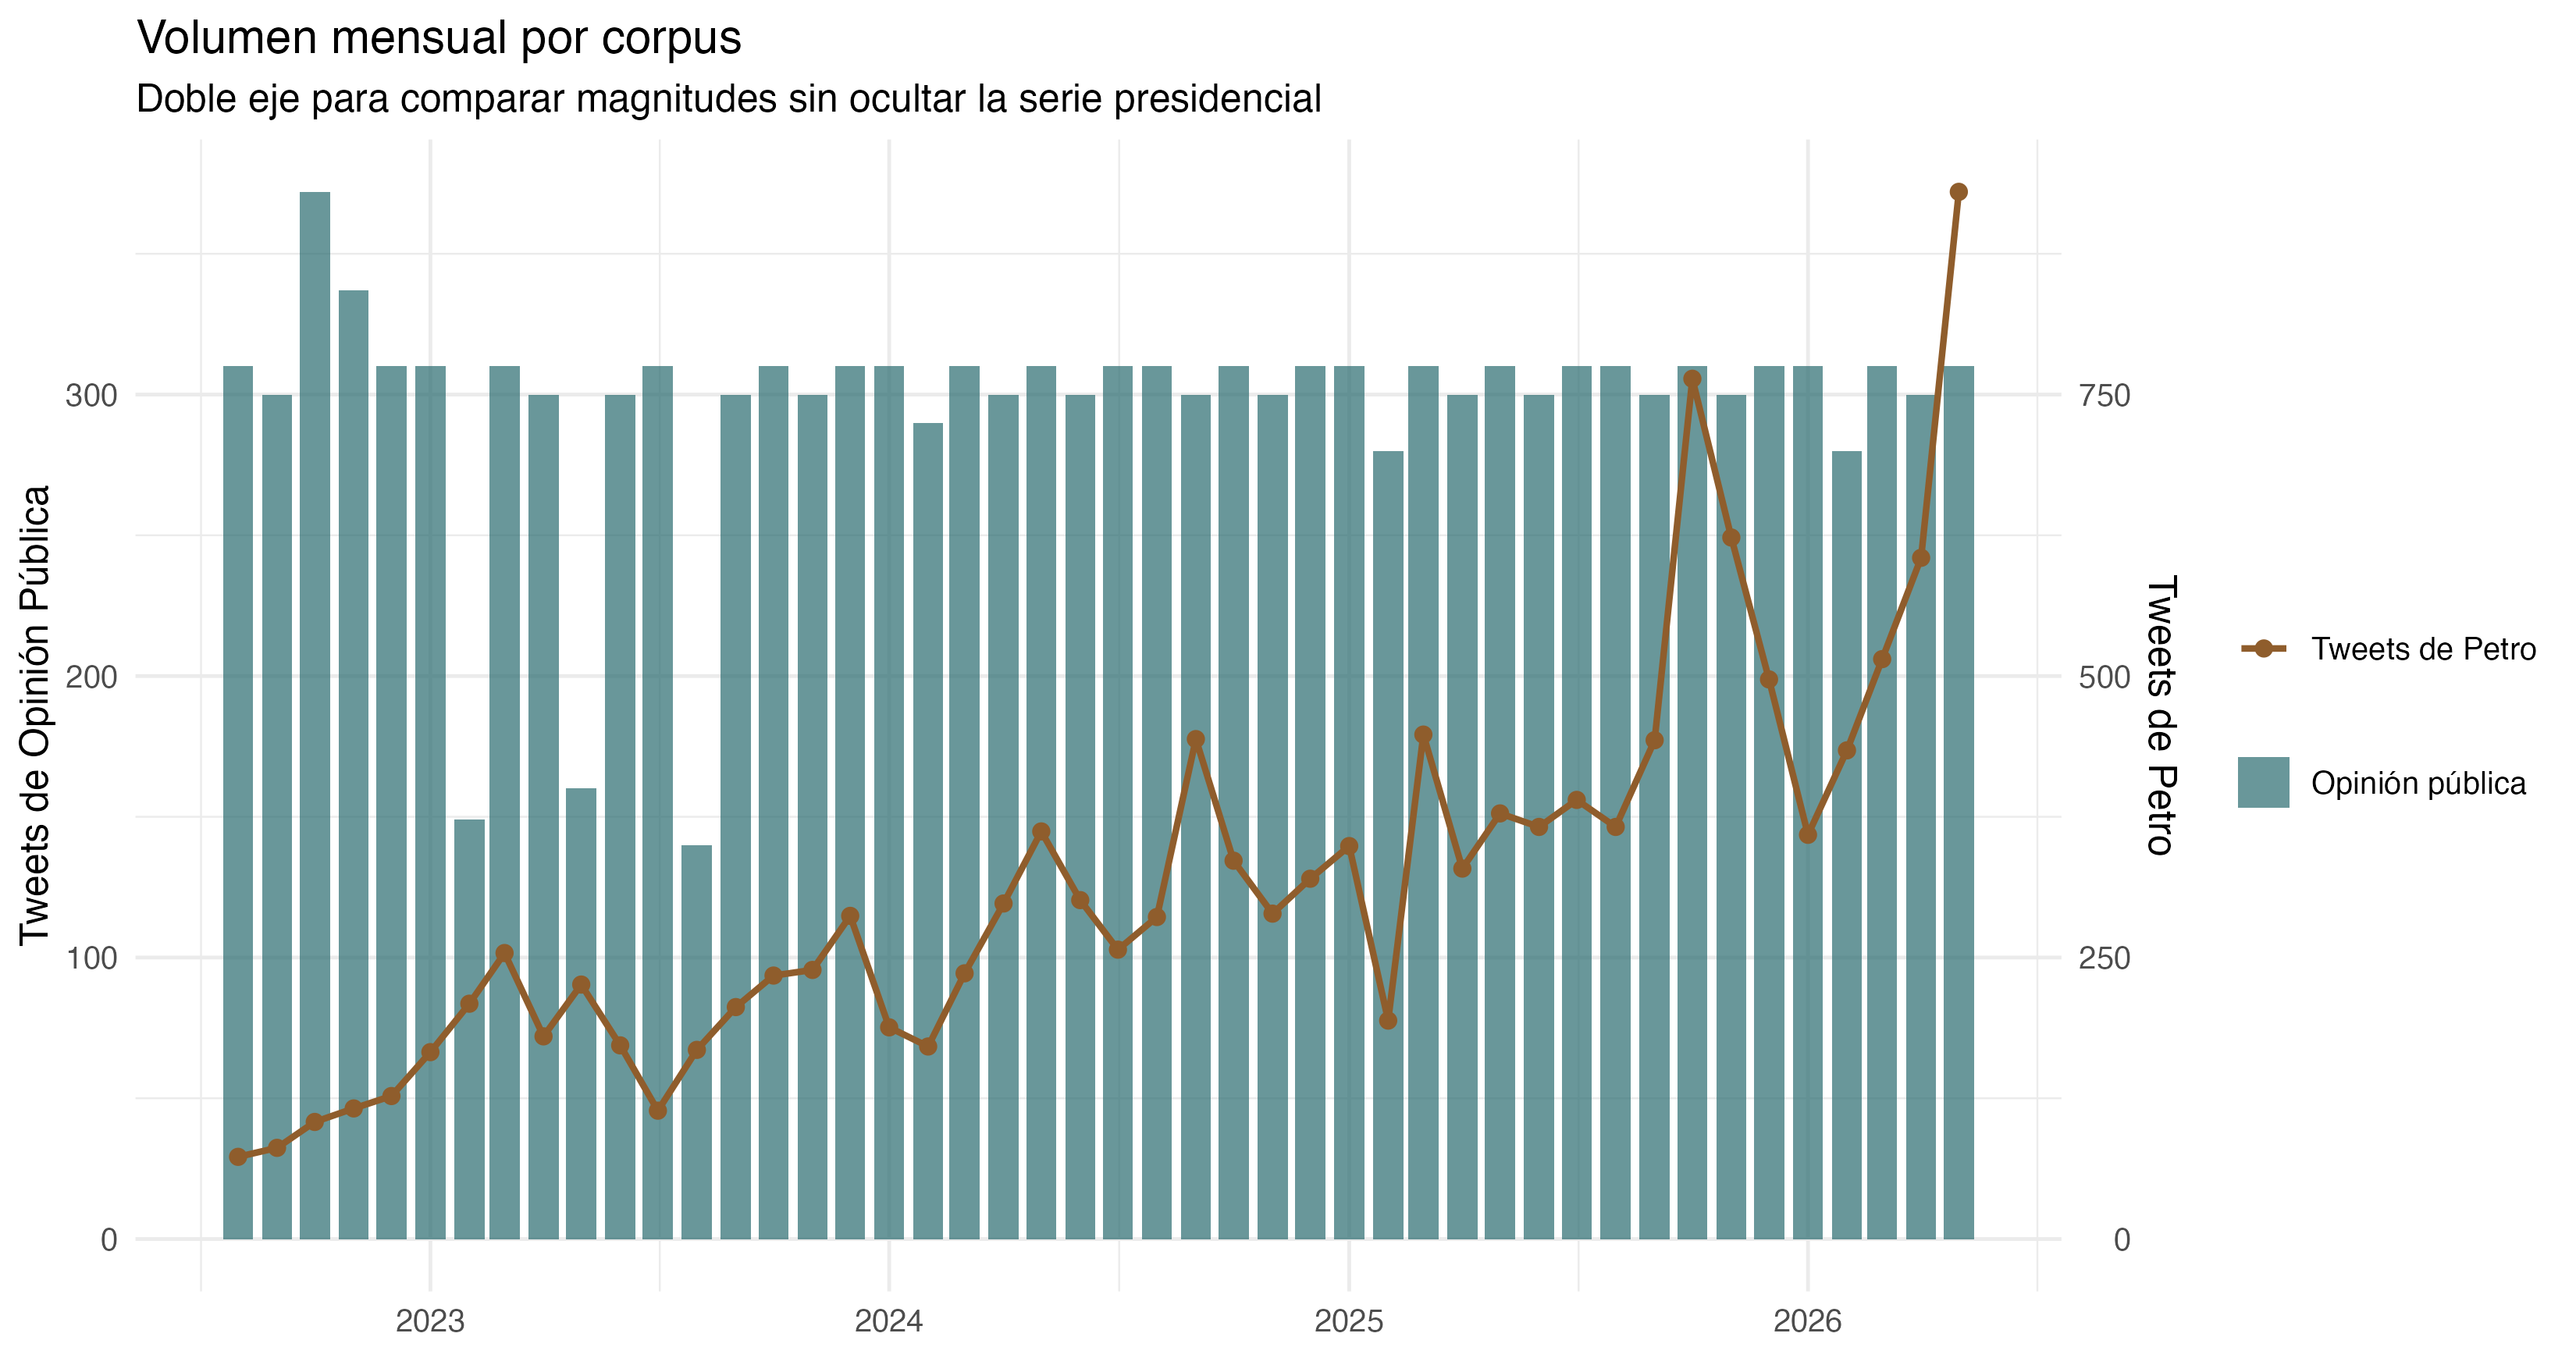
\includegraphics[width=0.9\linewidth,height=\textheight,keepaspectratio]{figures/comparacion_corpus_volumen.png}

}

\caption{\label{fig-corpus-volume}Volumen mensual comparado entre
conversación pública y tweets presidenciales.}

\end{figure}%

El análisis EDA de frecuencia presidencial muestra que
\texttt{@petrogustavo} no publica con una cadencia uniforme. La
actividad diaria contiene muchos días de baja producción y episodios
concentrados de alta intensidad; la agregación mensual revela un salto
pronunciado desde octubre de 2025, con picos en noviembre de 2025 y
durante los primeros meses de 2026. Por eso, en la unión con mercado no
basta contar tweets: también es necesario conservar la temporalidad,
diferenciar meses parciales y observar semanas con sobrecarga
comunicativa.

\begin{figure}

\centering{

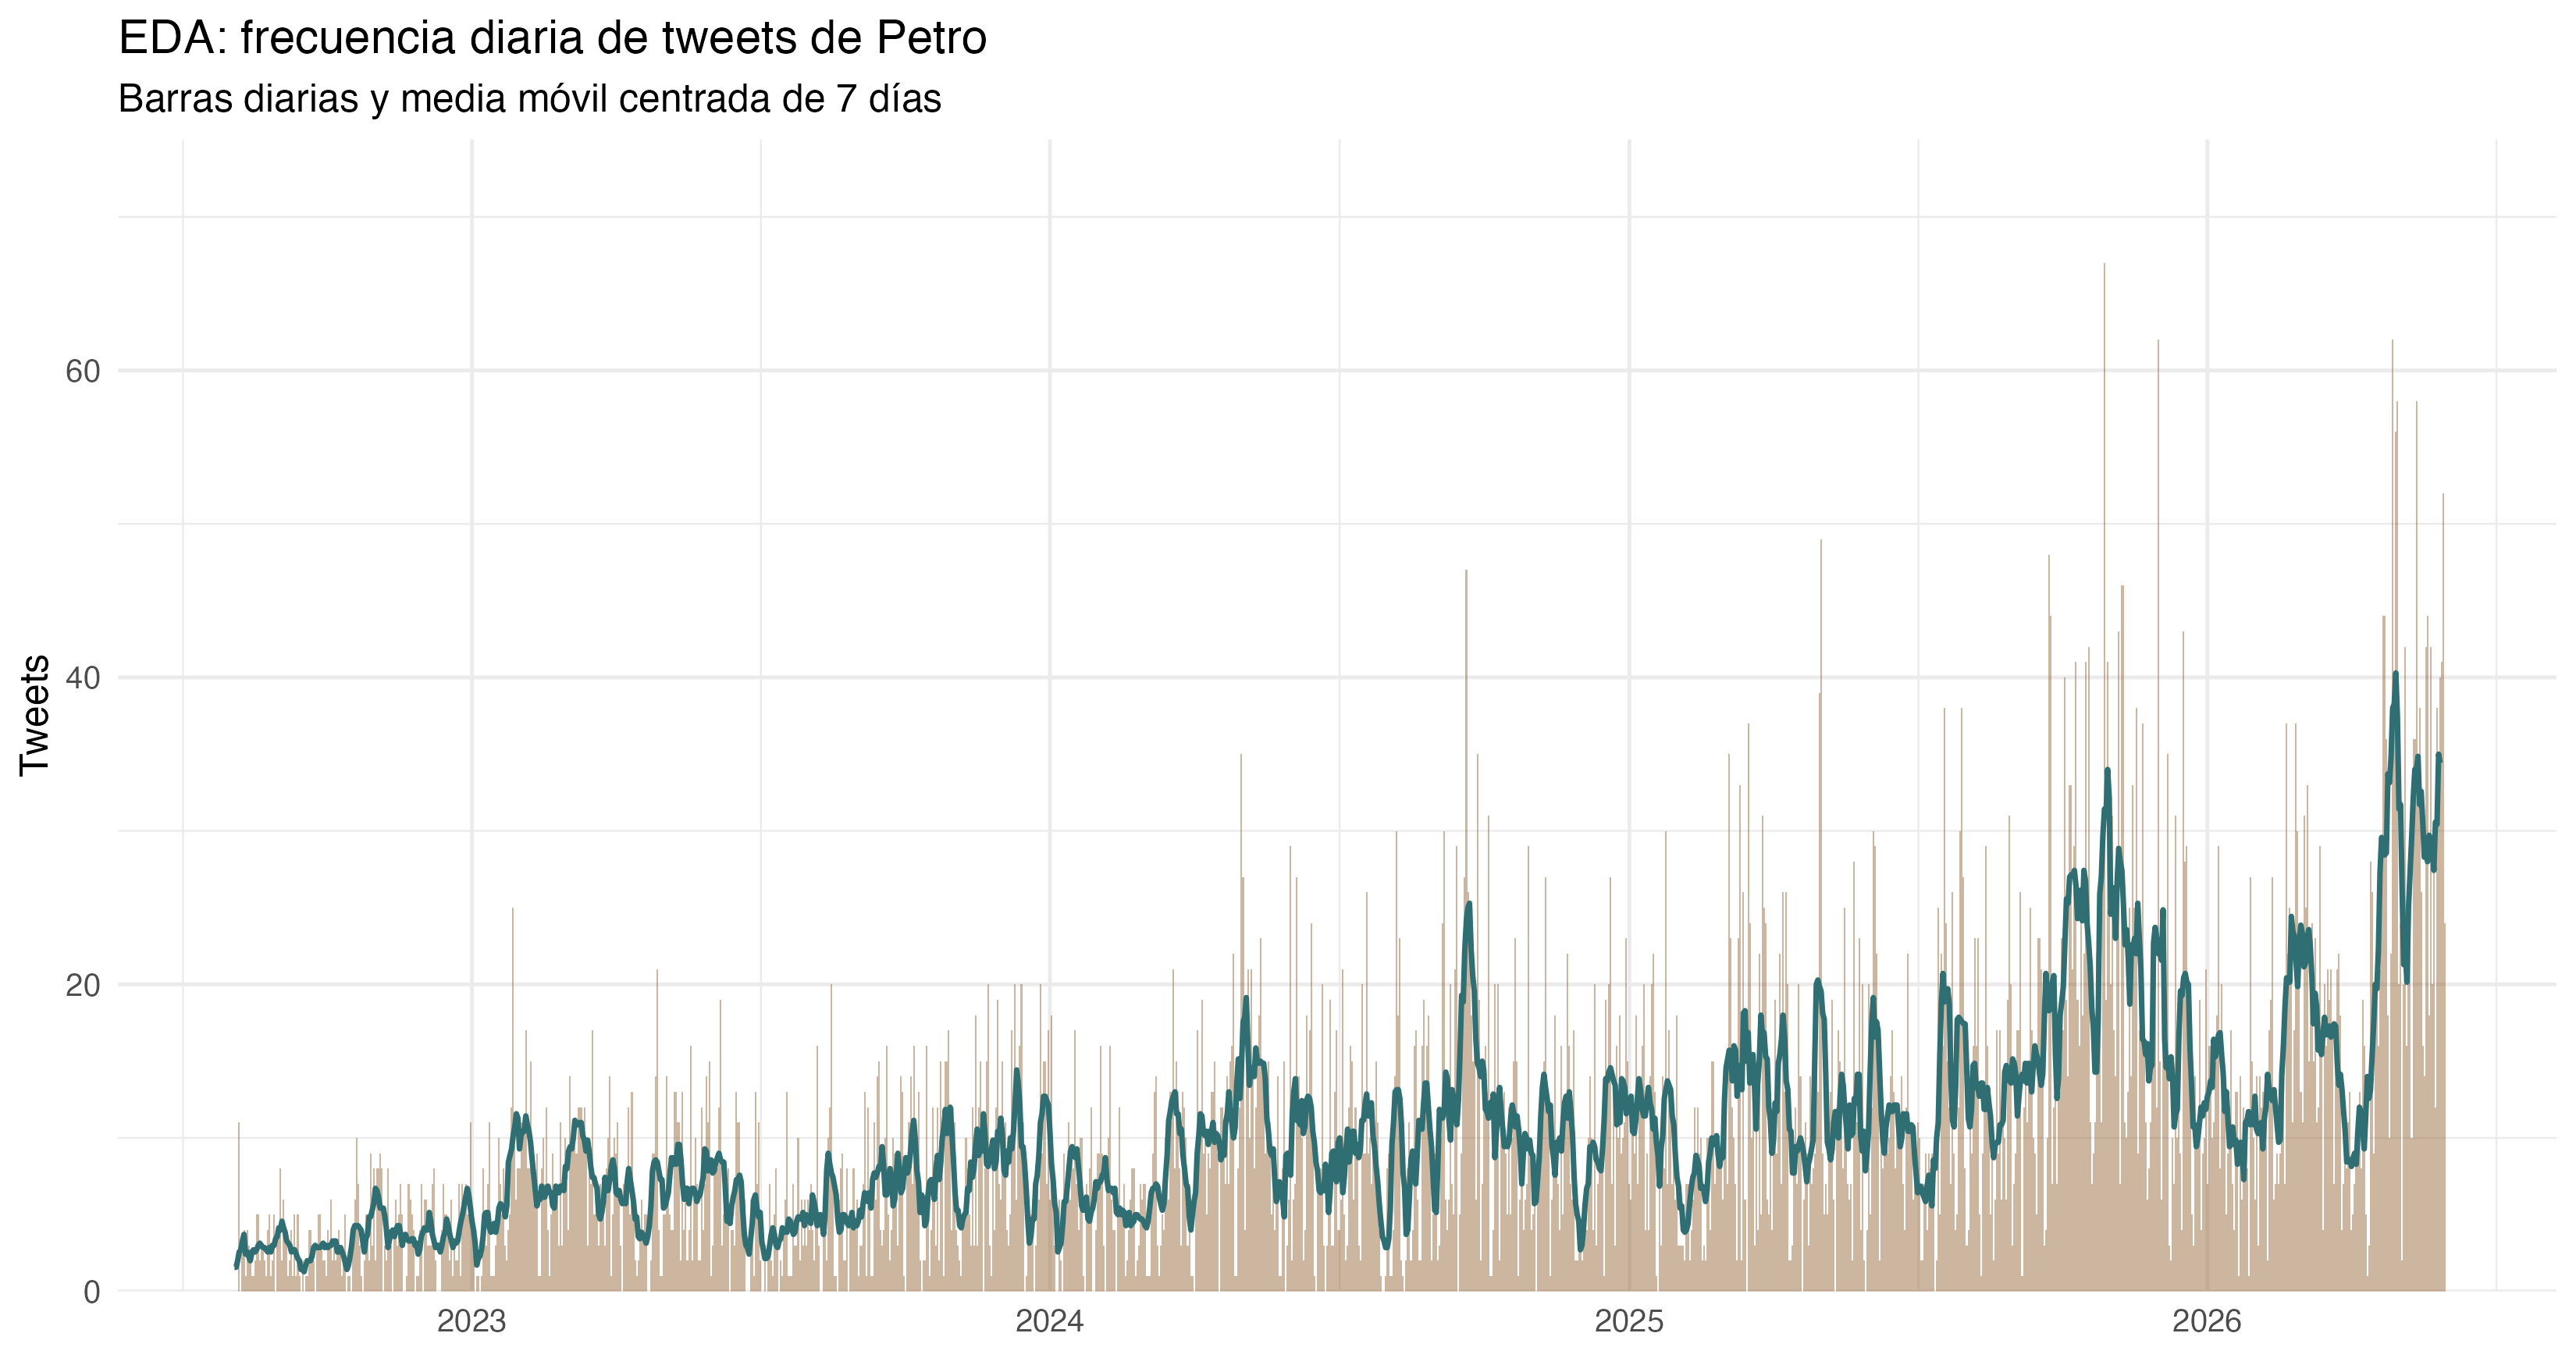
\includegraphics[width=0.9\linewidth,height=\textheight,keepaspectratio]{figures/eda_petro_tweets_diarios.png}

}

\caption{\label{fig-petro-daily-frequency}Frecuencia diaria de tweets
emitidos por \texttt{@petrogustavo}.}

\end{figure}%

\begin{figure}

\centering{

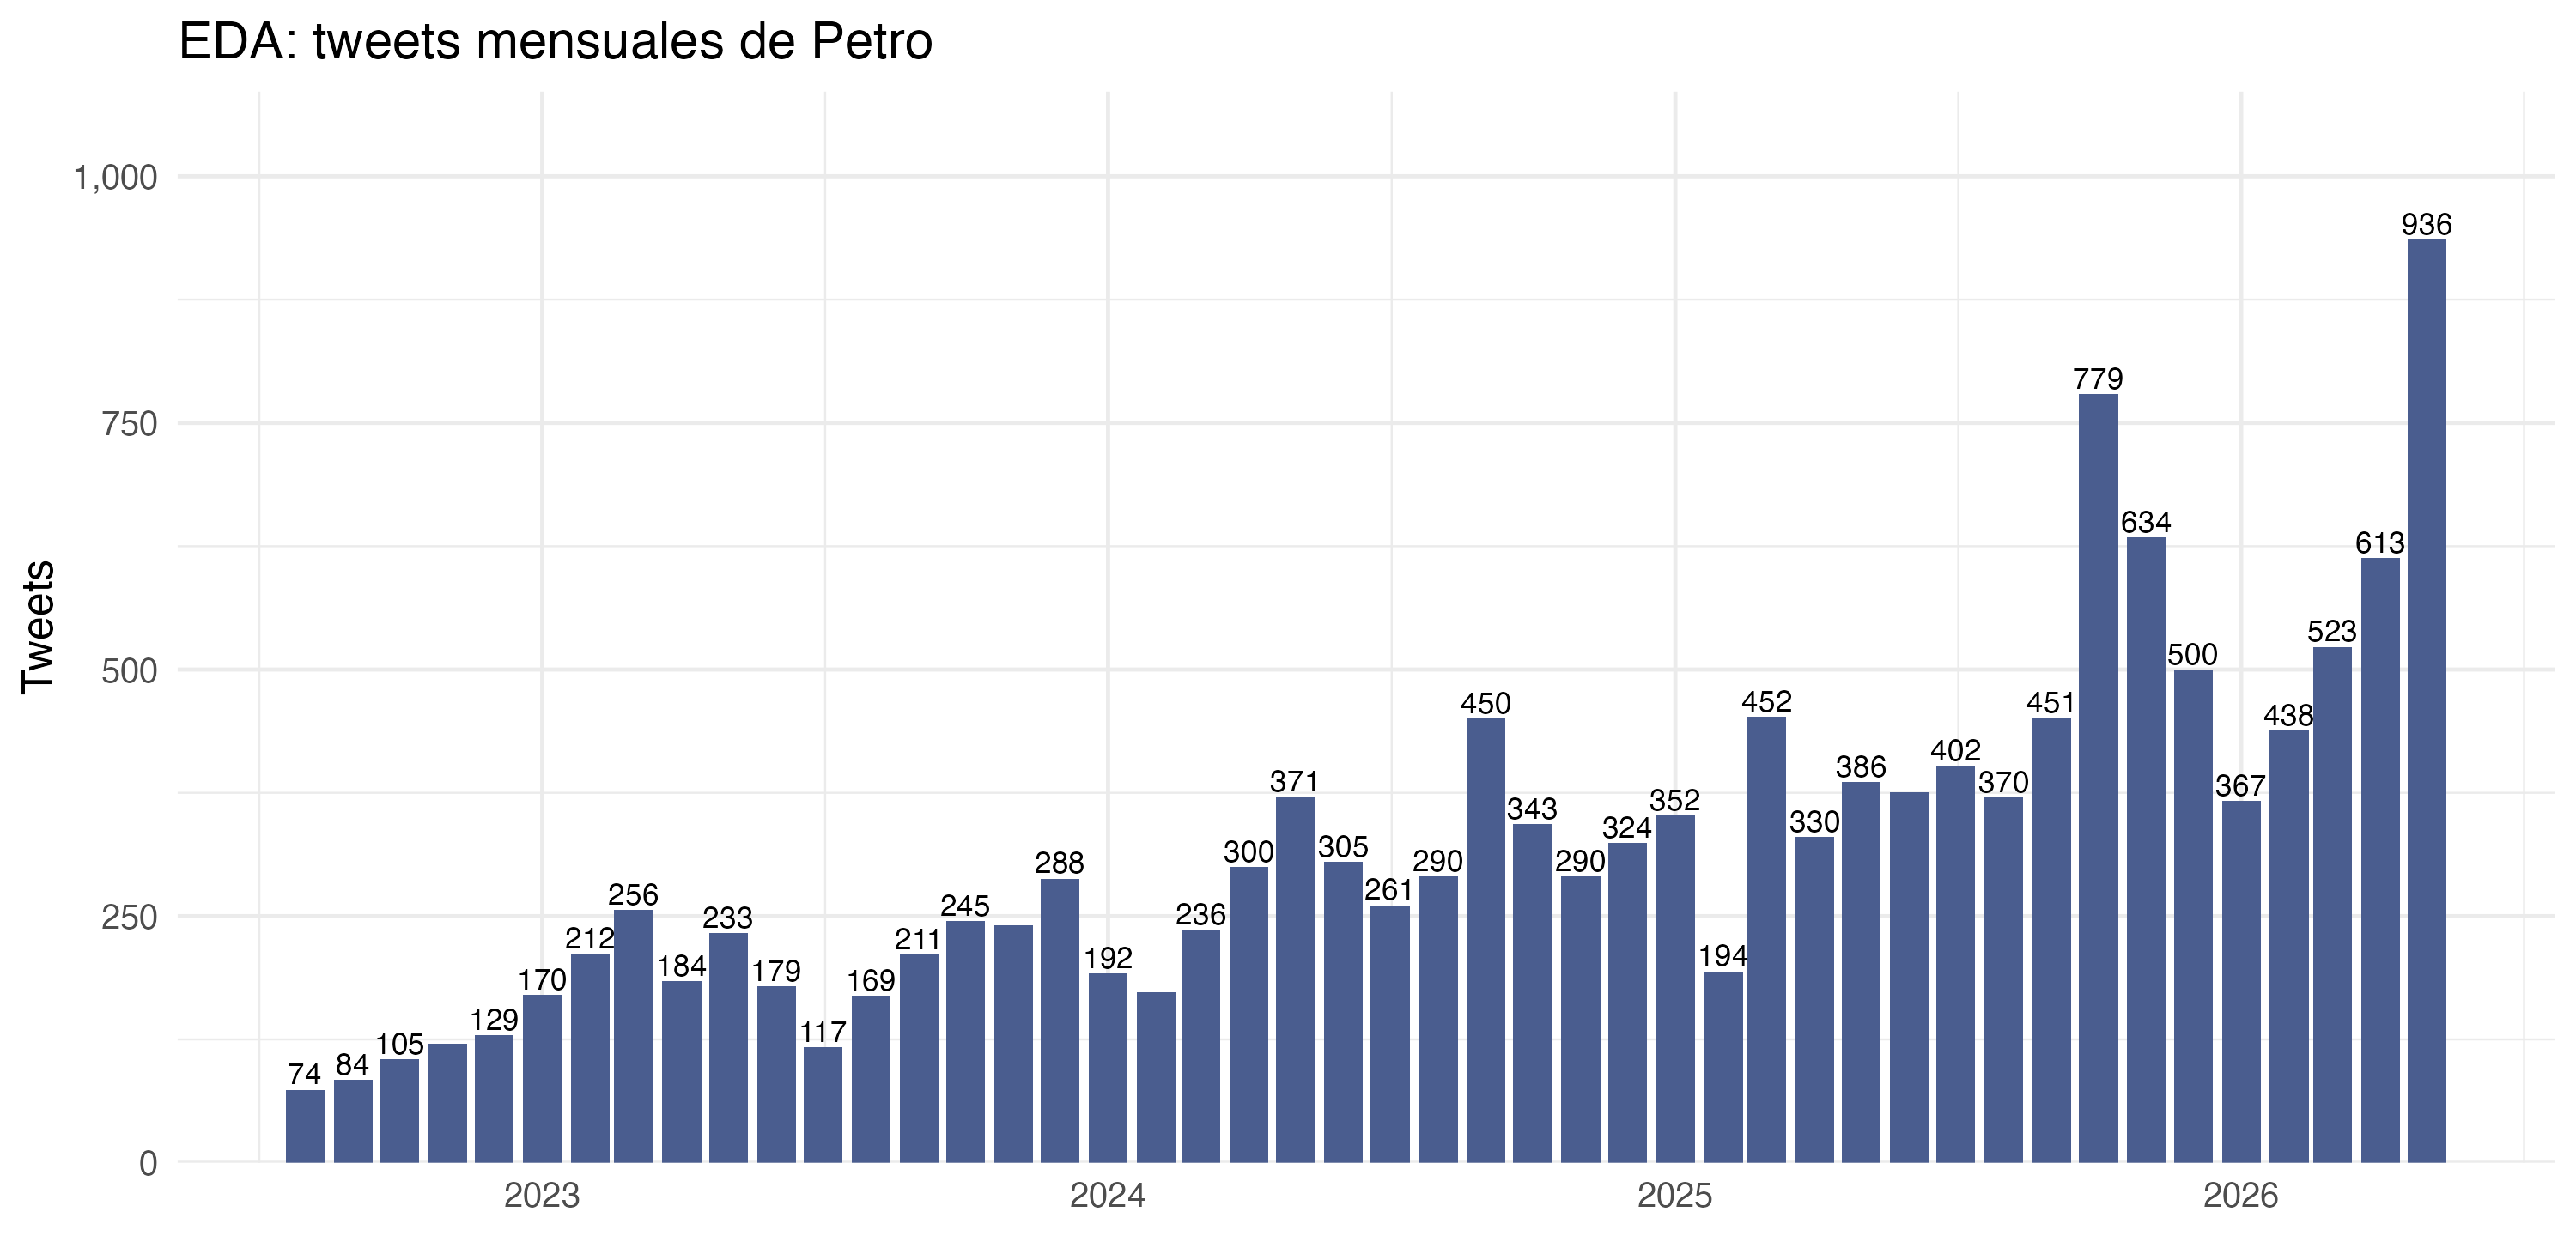
\includegraphics[width=0.85\linewidth,height=\textheight,keepaspectratio]{figures/eda_petro_tweets_mensuales.png}

}

\caption{\label{fig-petro-monthly-frequency}Frecuencia mensual de tweets
emitidos por \texttt{@petrogustavo}.}

\end{figure}%

\begin{figure}

\centering{

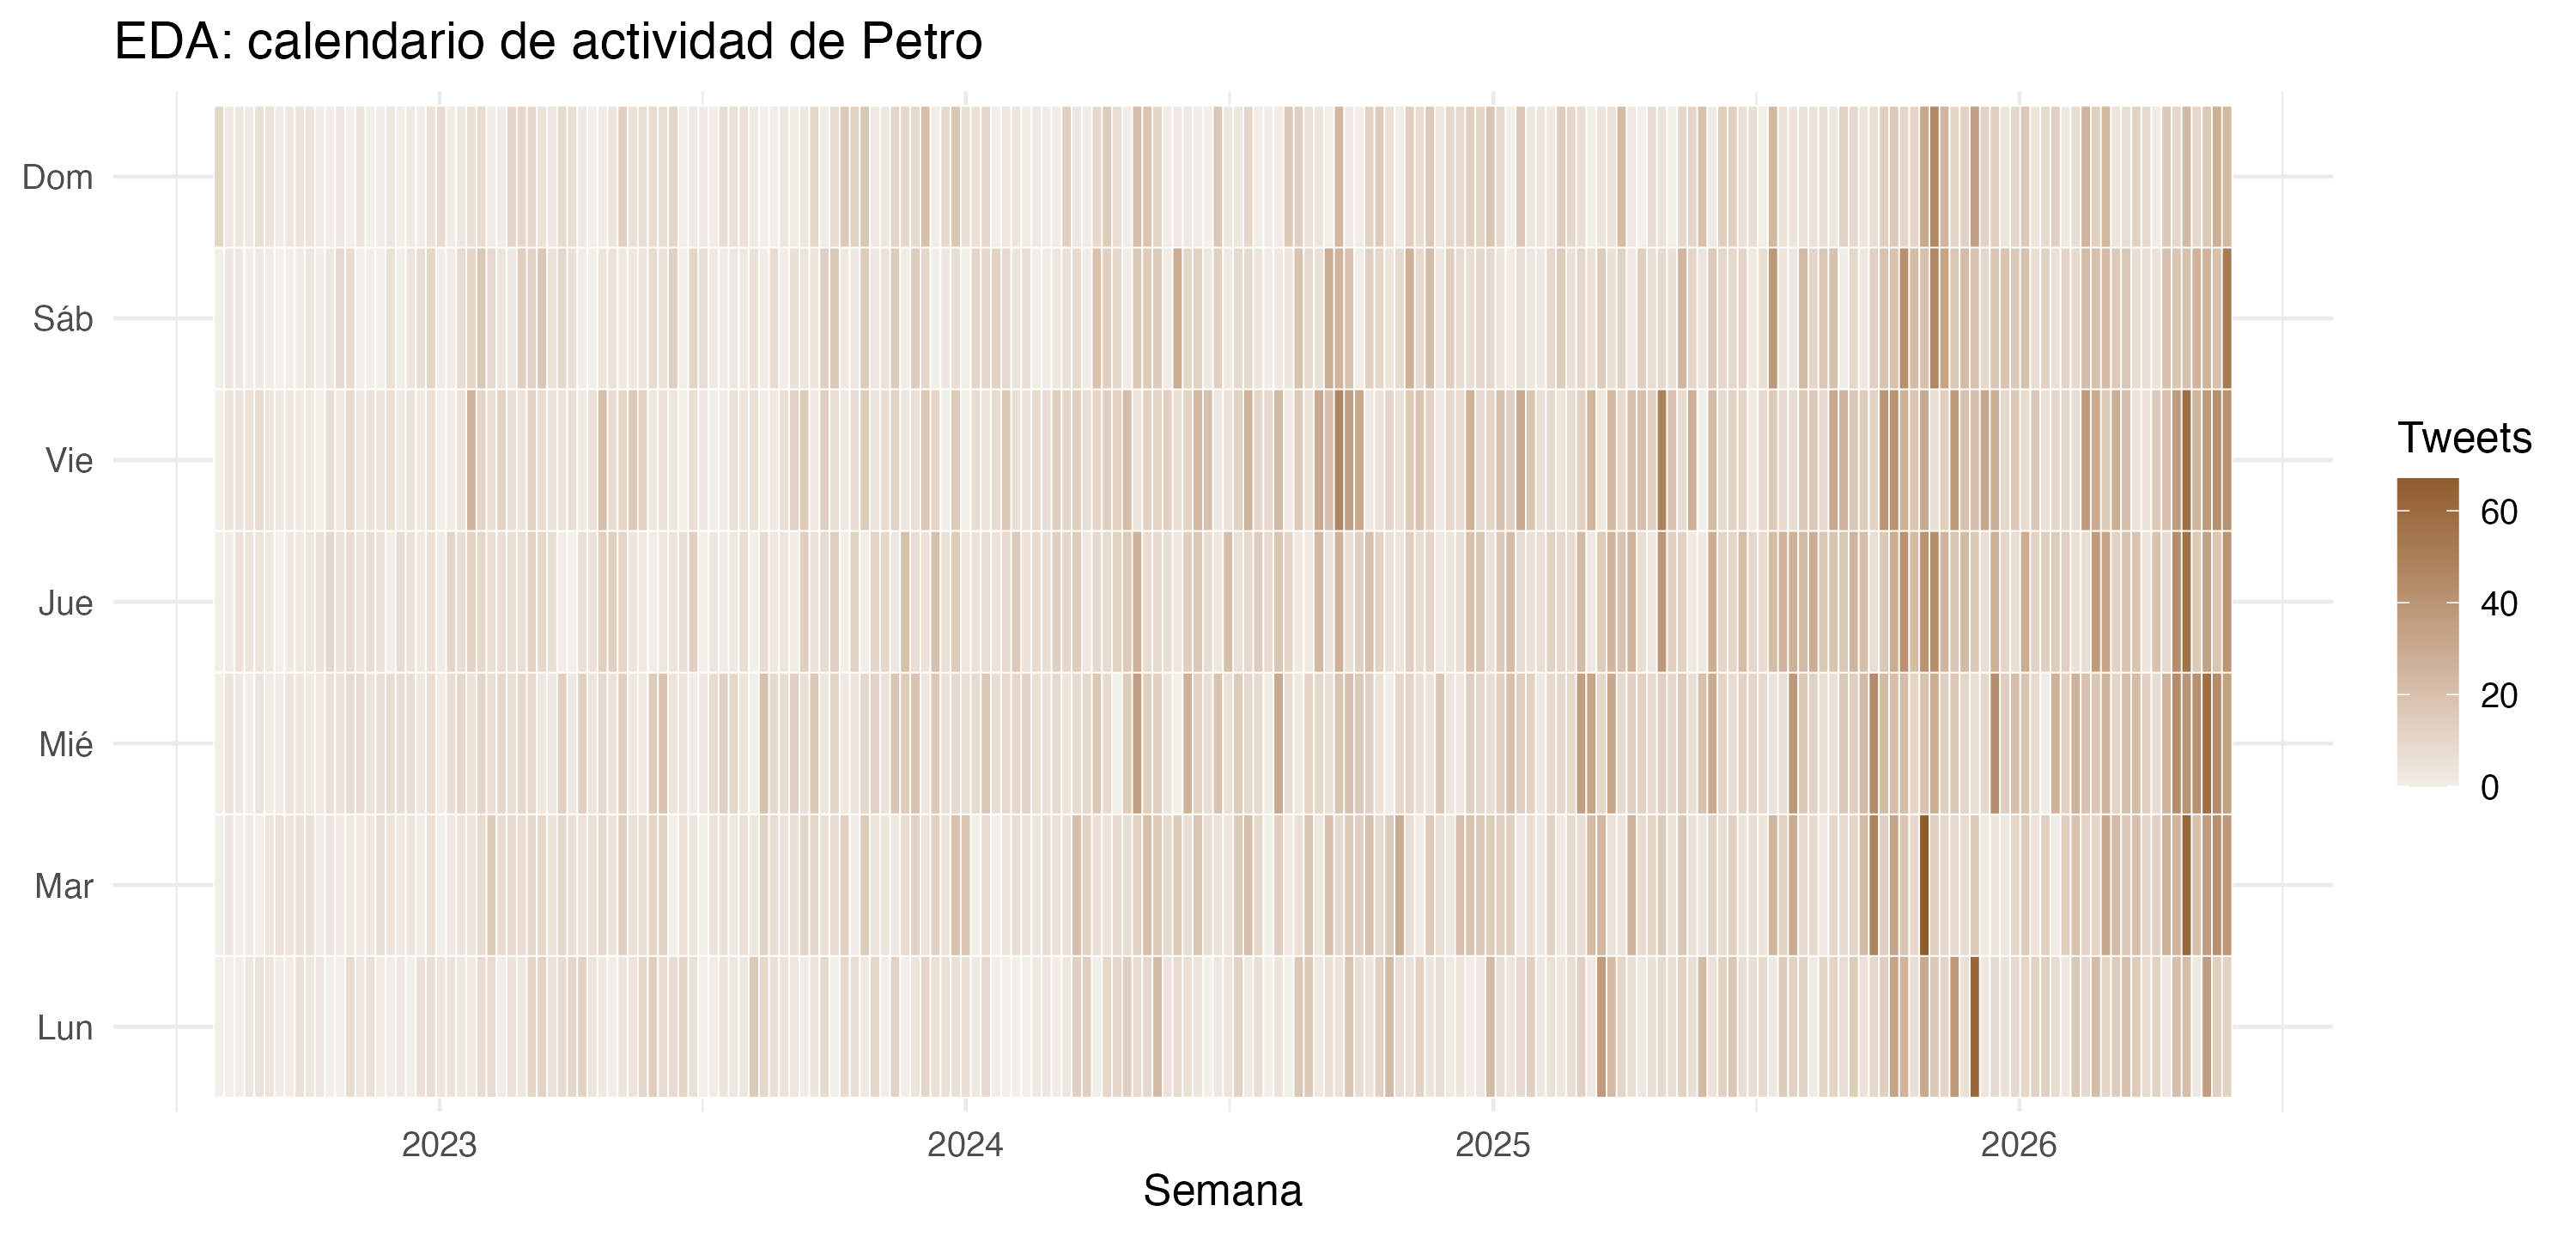
\includegraphics[width=0.9\linewidth,height=\textheight,keepaspectratio]{figures/eda_petro_calendario_actividad.png}

}

\caption{\label{fig-petro-calendar-frequency}Calendario de actividad de
tweets emitidos por \texttt{@petrogustavo}.}

\end{figure}%

Los resultados de hashtags y menciones conservan un hallazgo central del
paper original: la conversación alrededor de Petro es polarizada.
Existen etiquetas de apoyo, oposición, denuncia, movilización y crítica
institucional. La actualización muestra que esa polarización no se
limita a lenguaje electoral; también aparece alrededor de reforma de
salud, laboral, pensional, tributaria, paz total, tipo de cambio,
mercado accionario y confianza en la administración.

\begin{figure}

\centering{

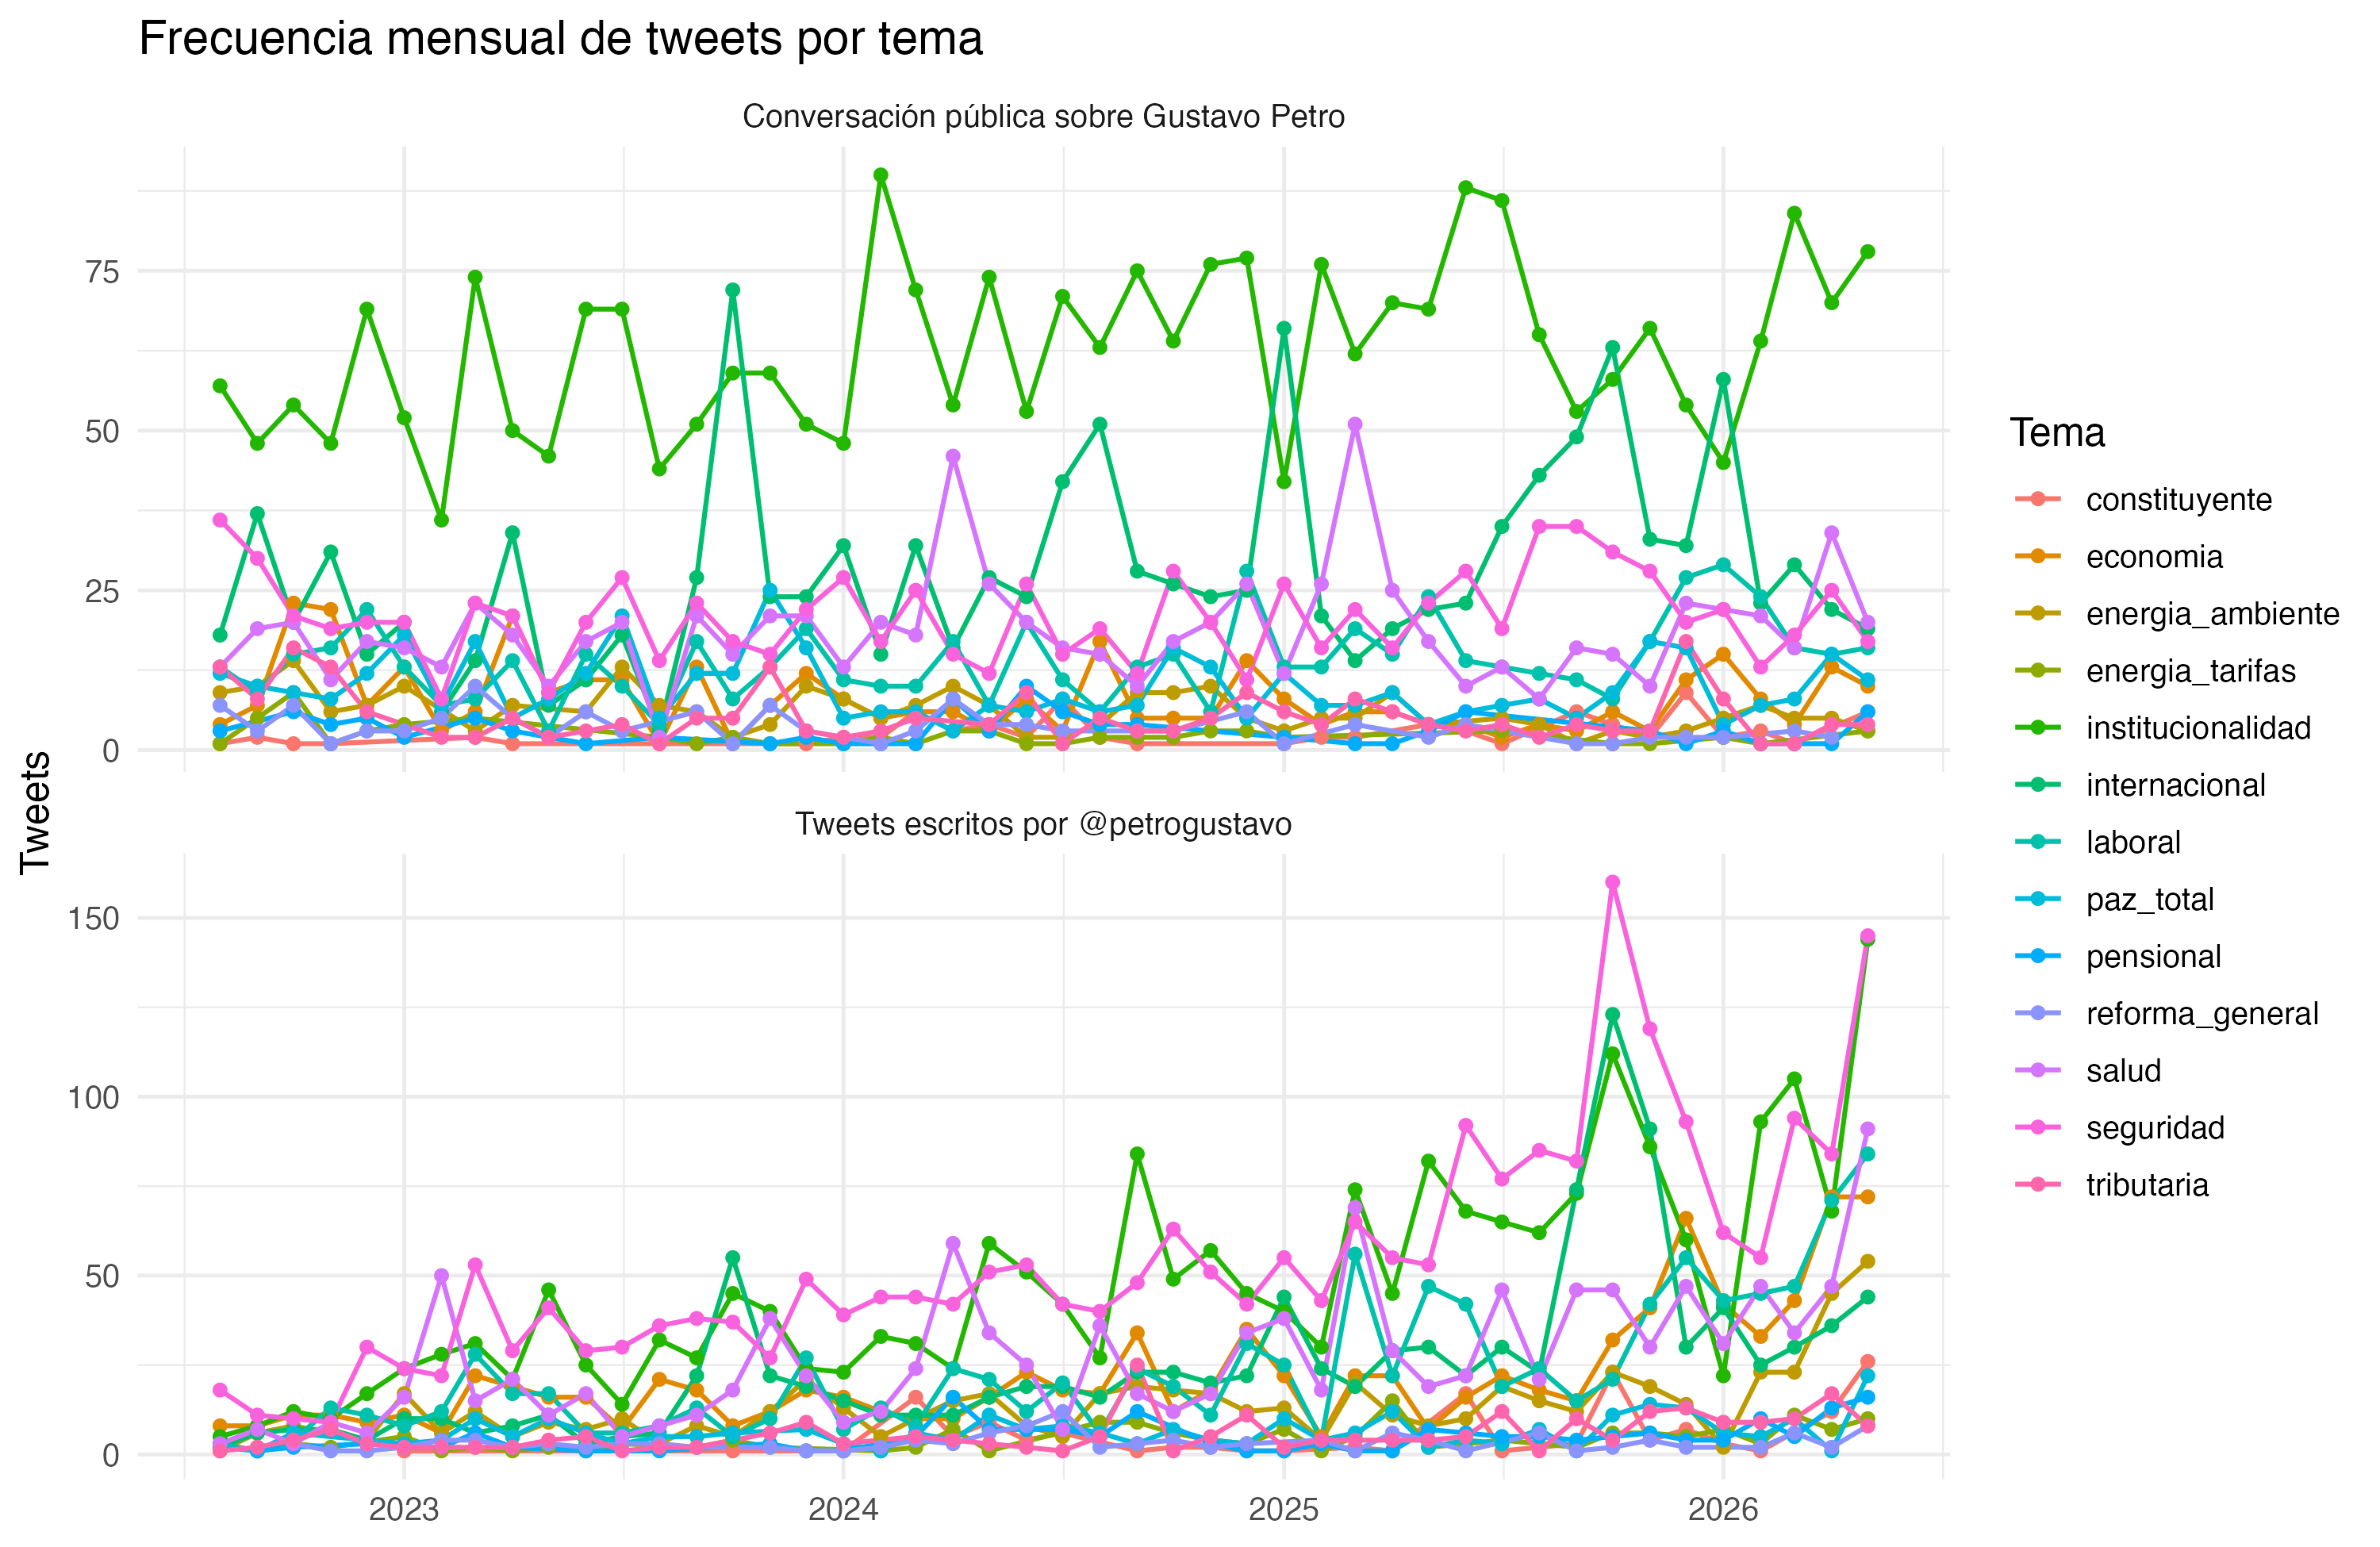
\includegraphics[width=0.9\linewidth,height=\textheight,keepaspectratio]{figures/frecuencia_tweets_mensual.png}

}

\caption{\label{fig-frequency}Frecuencia mensual de tweets por tema de
política pública.}

\end{figure}%

Las redes calculadas con \texttt{quanteda} refuerzan esta lectura. La
red global de hashtags concentra etiquetas políticas y coyunturales que
se conectan por coaparición dentro de tweets, mientras que la red de
menciones muestra actores, cuentas institucionales, medios y usuarios
que organizan la conversación. Al separarlas por corpus, el contraste es
sustantivo: \texttt{opinion} captura una discusión pública más densa y
confrontacional; \texttt{presidente} es más selectivo y permite ver el
repertorio de etiquetas y cuentas que acompañan al discurso directo.

\begin{figure}

\centering{

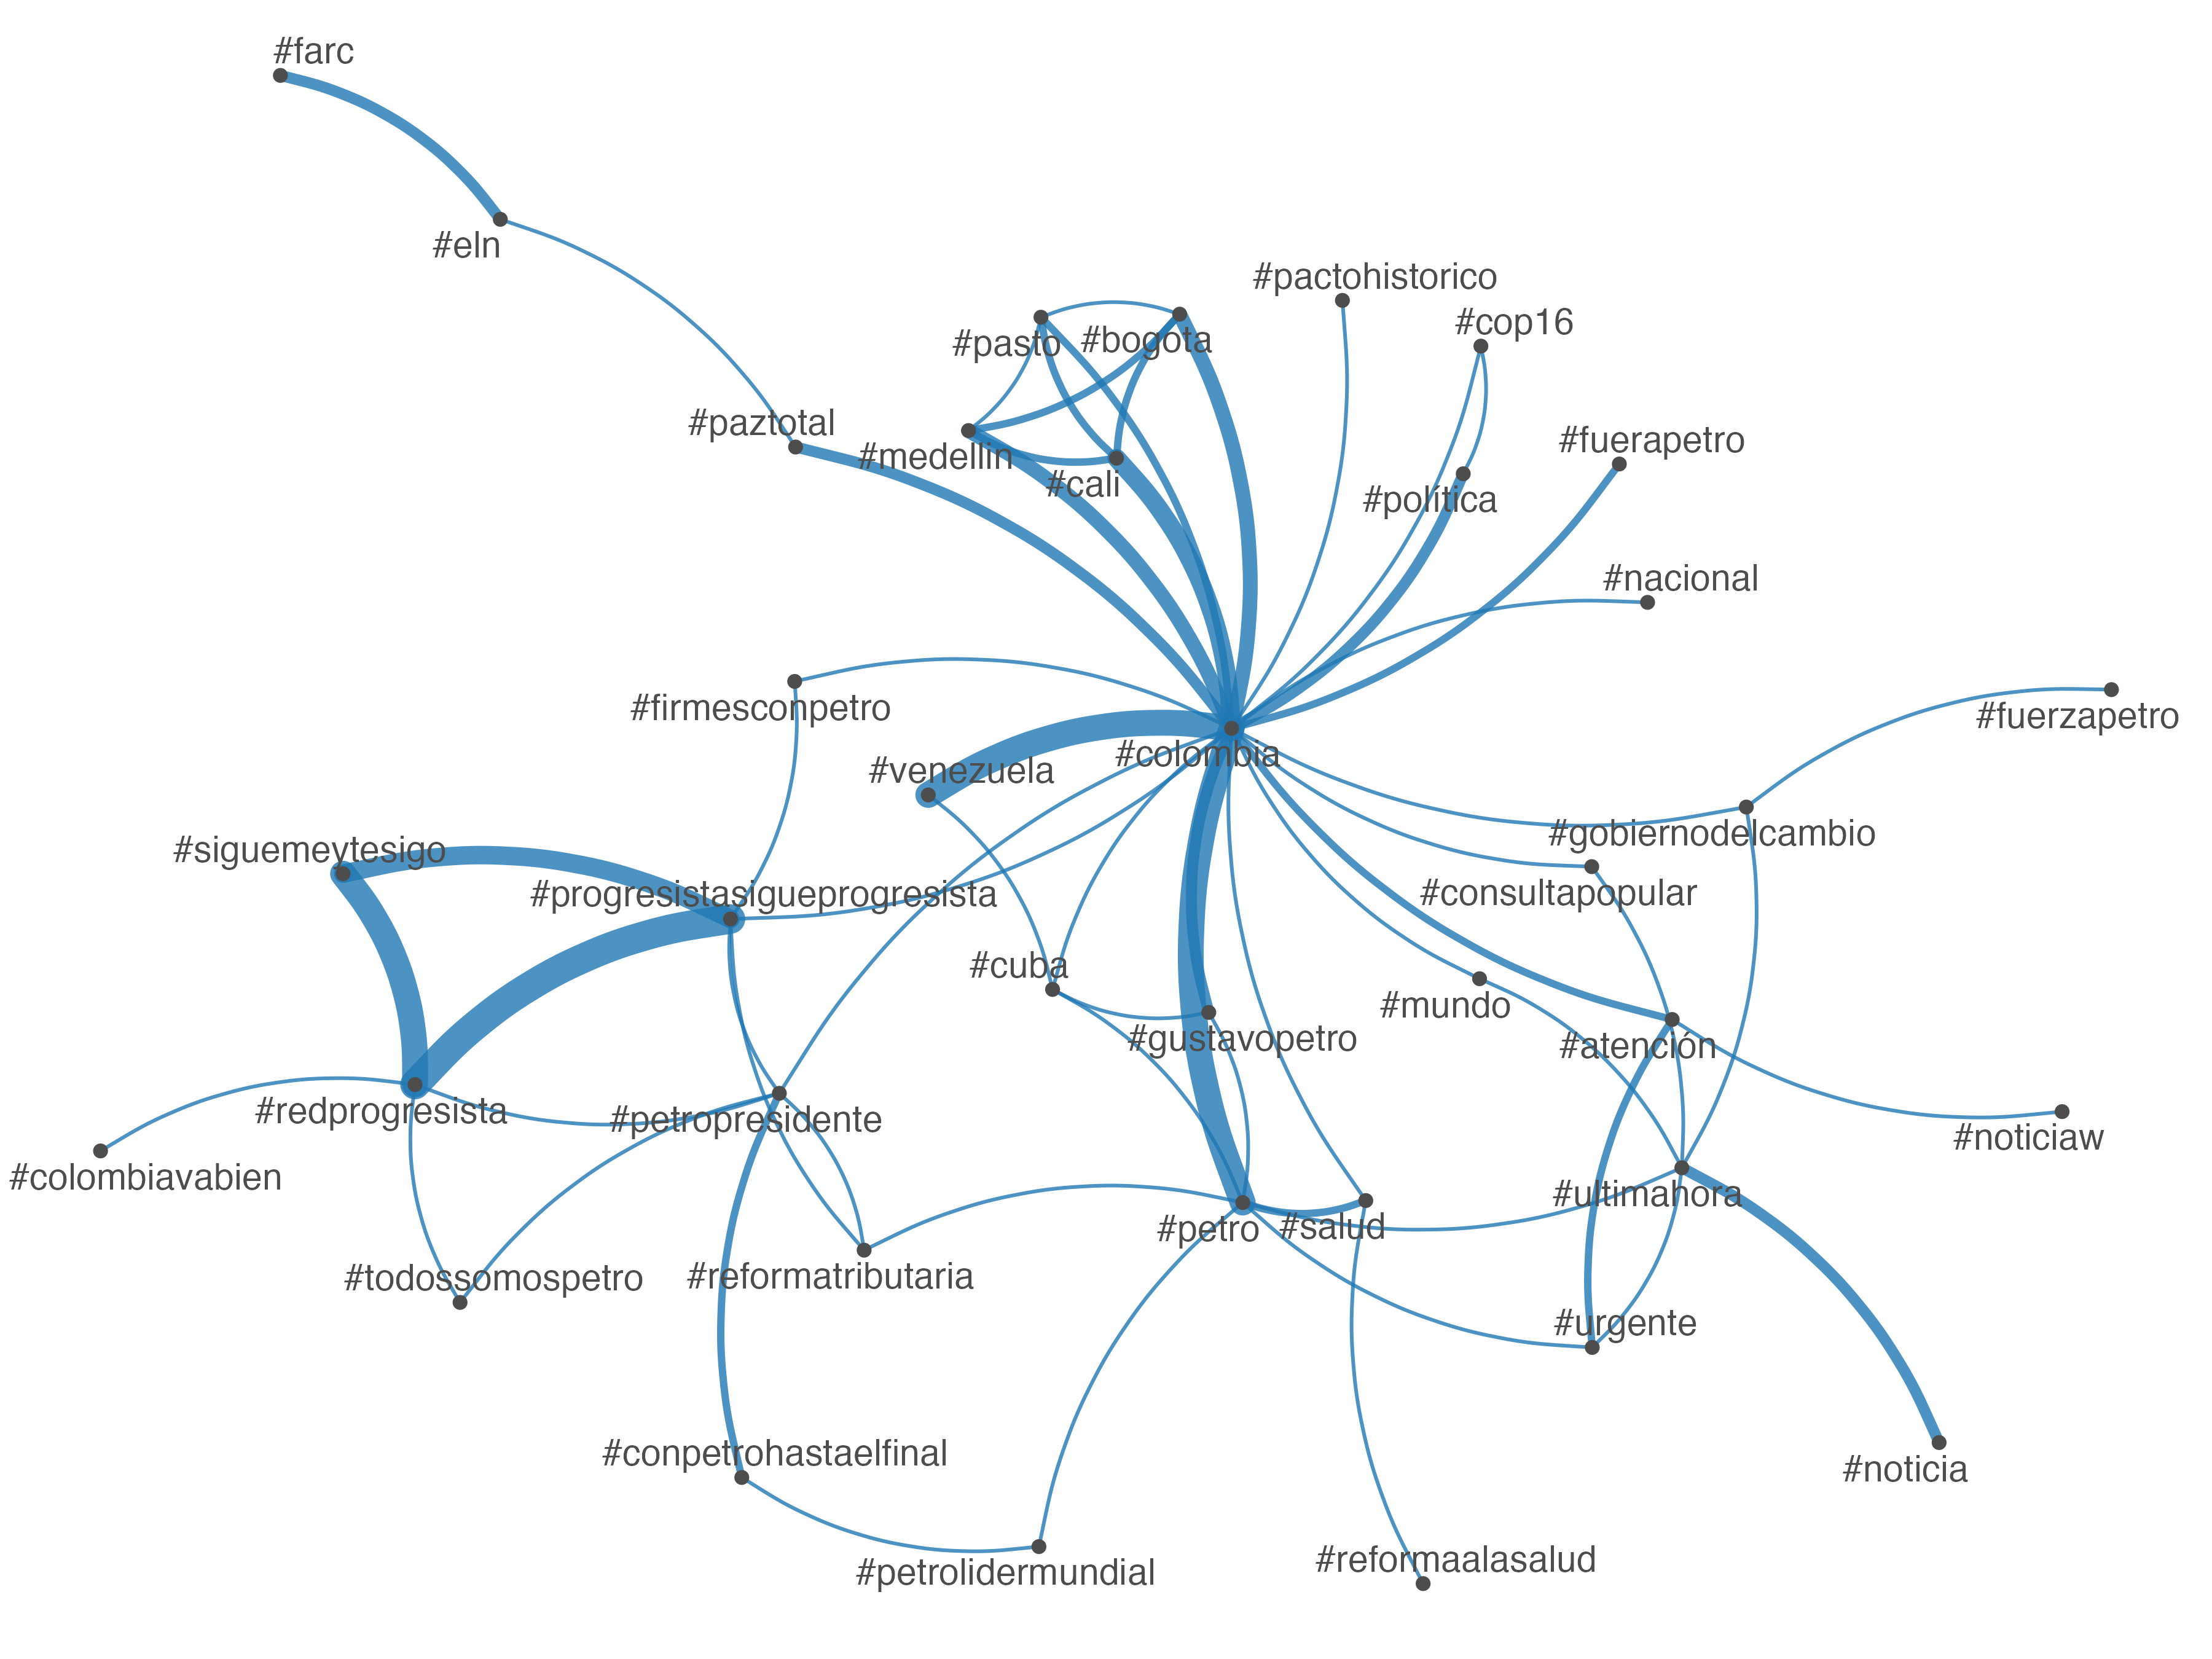
\includegraphics[width=0.9\linewidth,height=\textheight,keepaspectratio]{figures/red_hashtags_quanteda.png}

}

\caption{\label{fig-quanteda-hashtags}Red de hashtags con estilo
\texttt{quanteda} para el corpus completo.}

\end{figure}%

\begin{figure}

\centering{

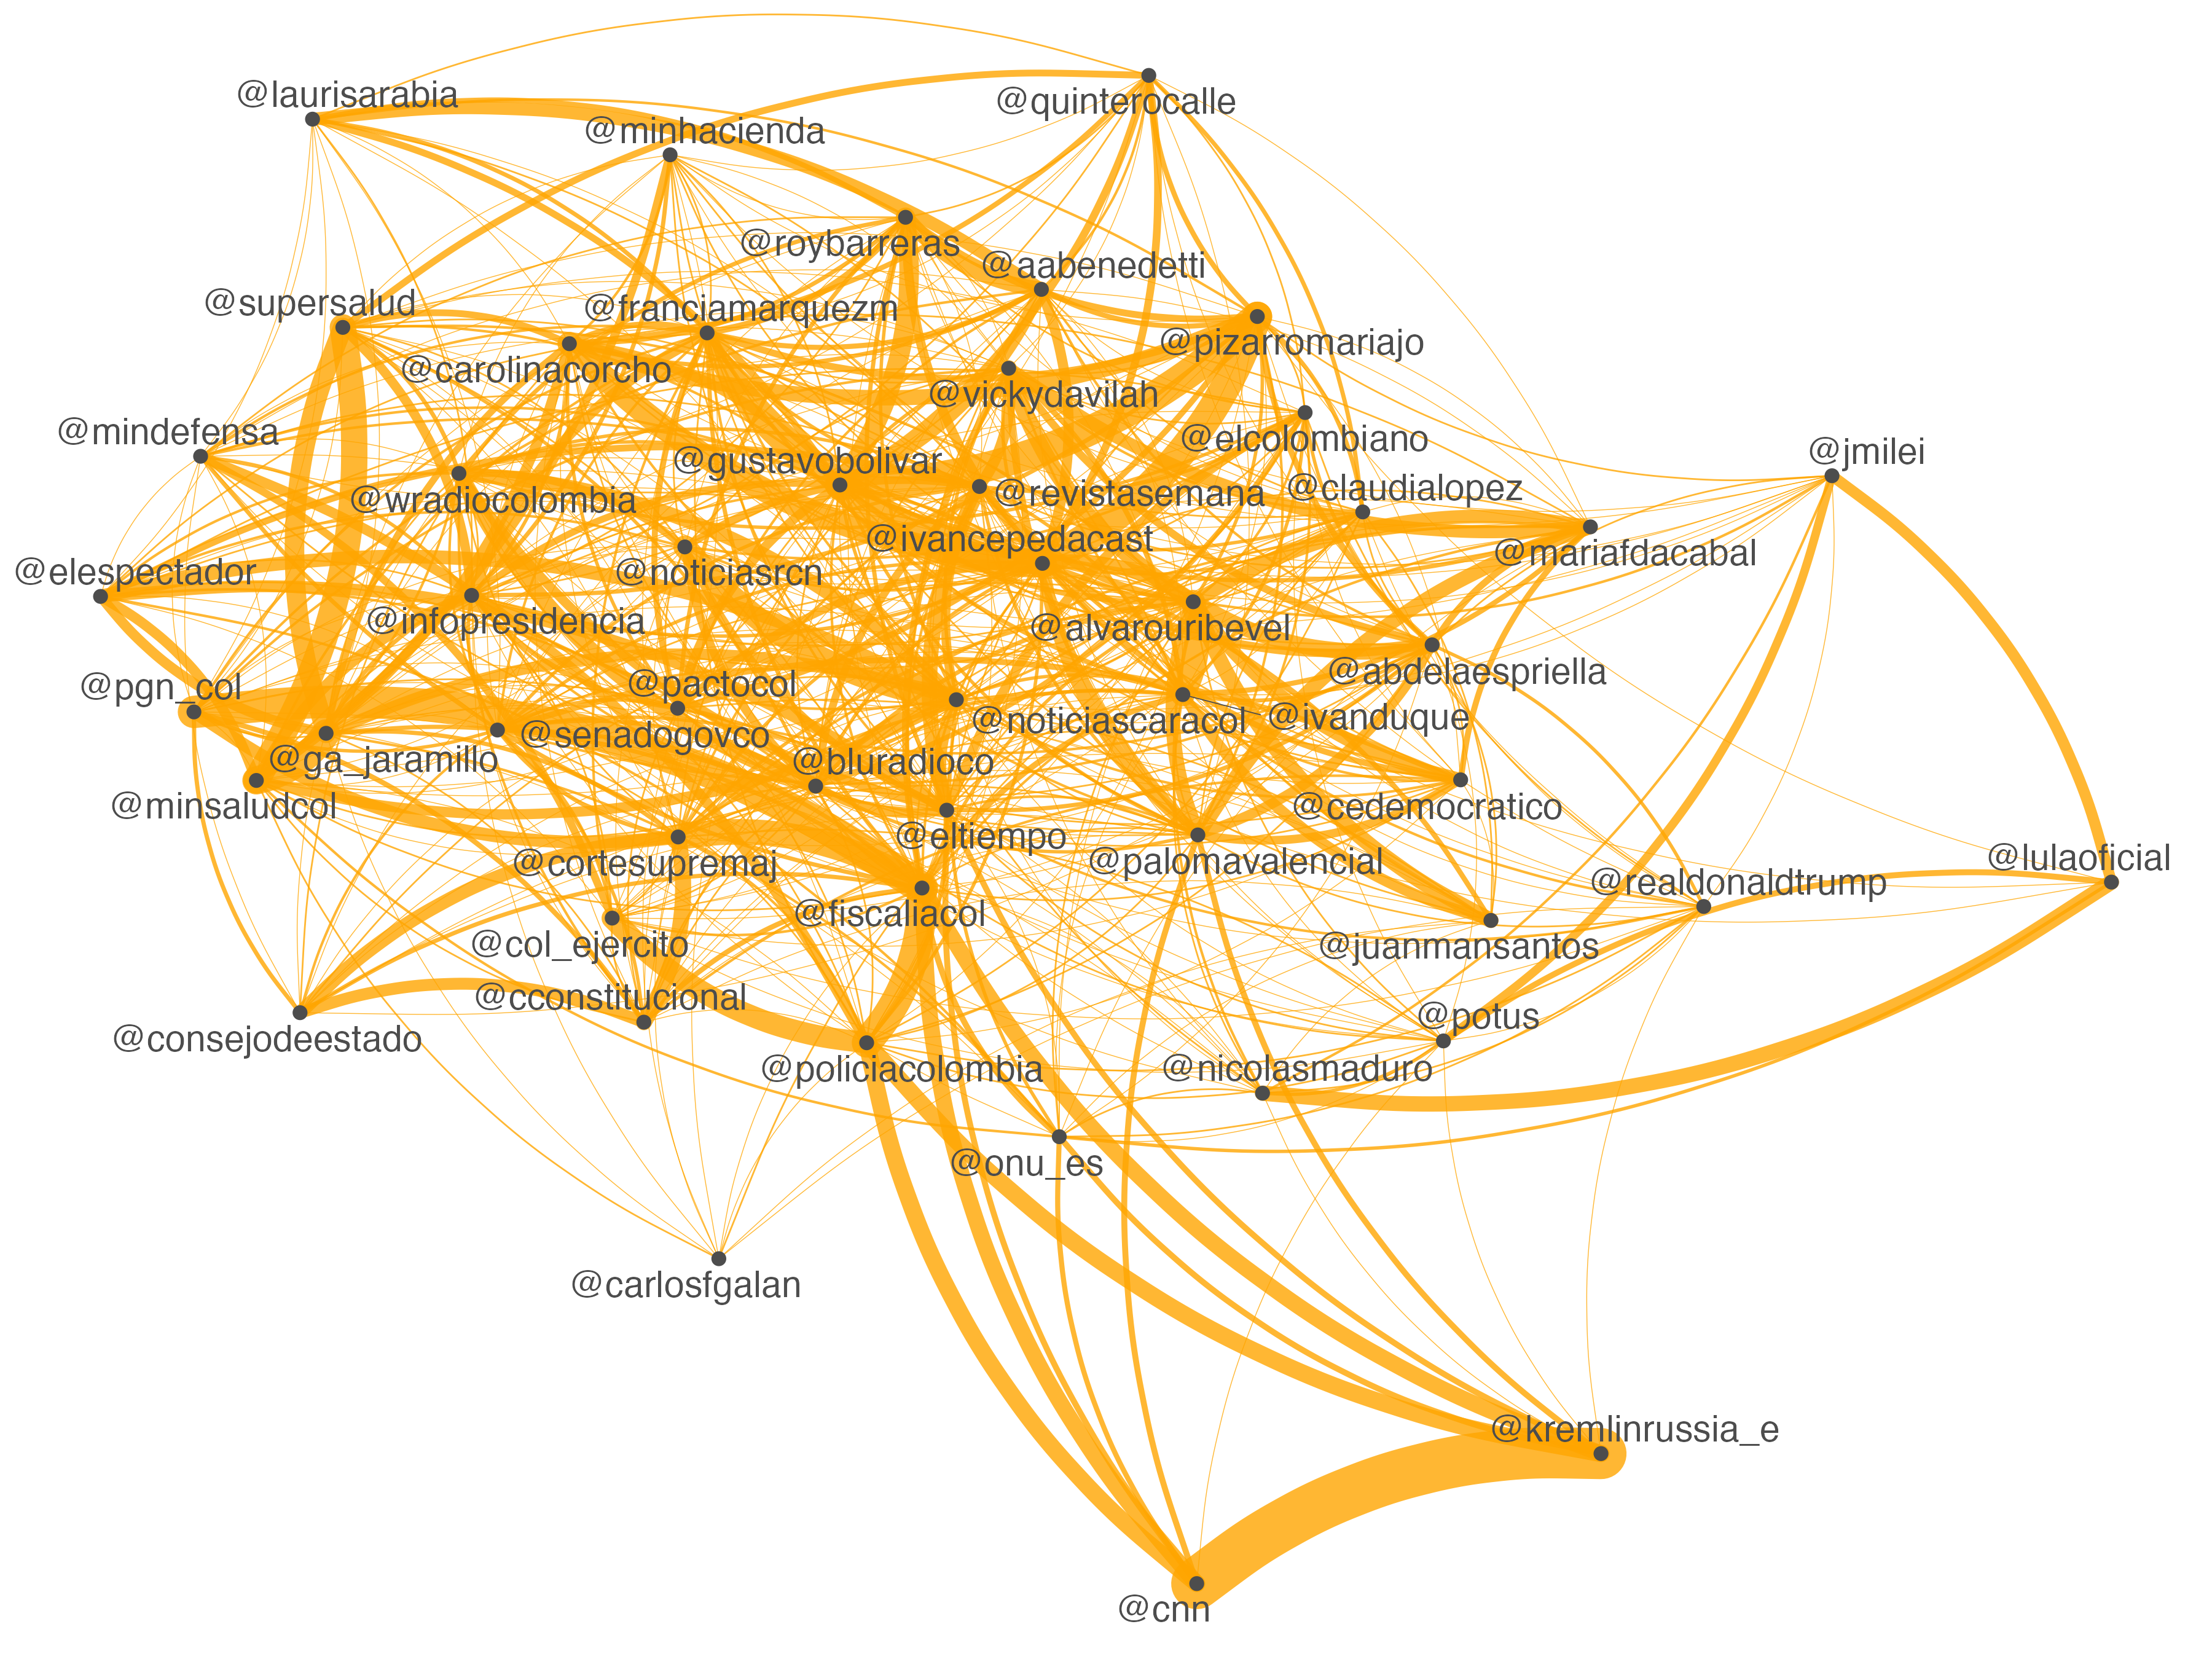
\includegraphics[width=0.9\linewidth,height=\textheight,keepaspectratio]{figures/red_menciones_quanteda.png}

}

\caption{\label{fig-quanteda-mentions}Red de menciones con estilo
\texttt{quanteda} para el corpus completo.}

\end{figure}%

\begin{figure}

\centering{

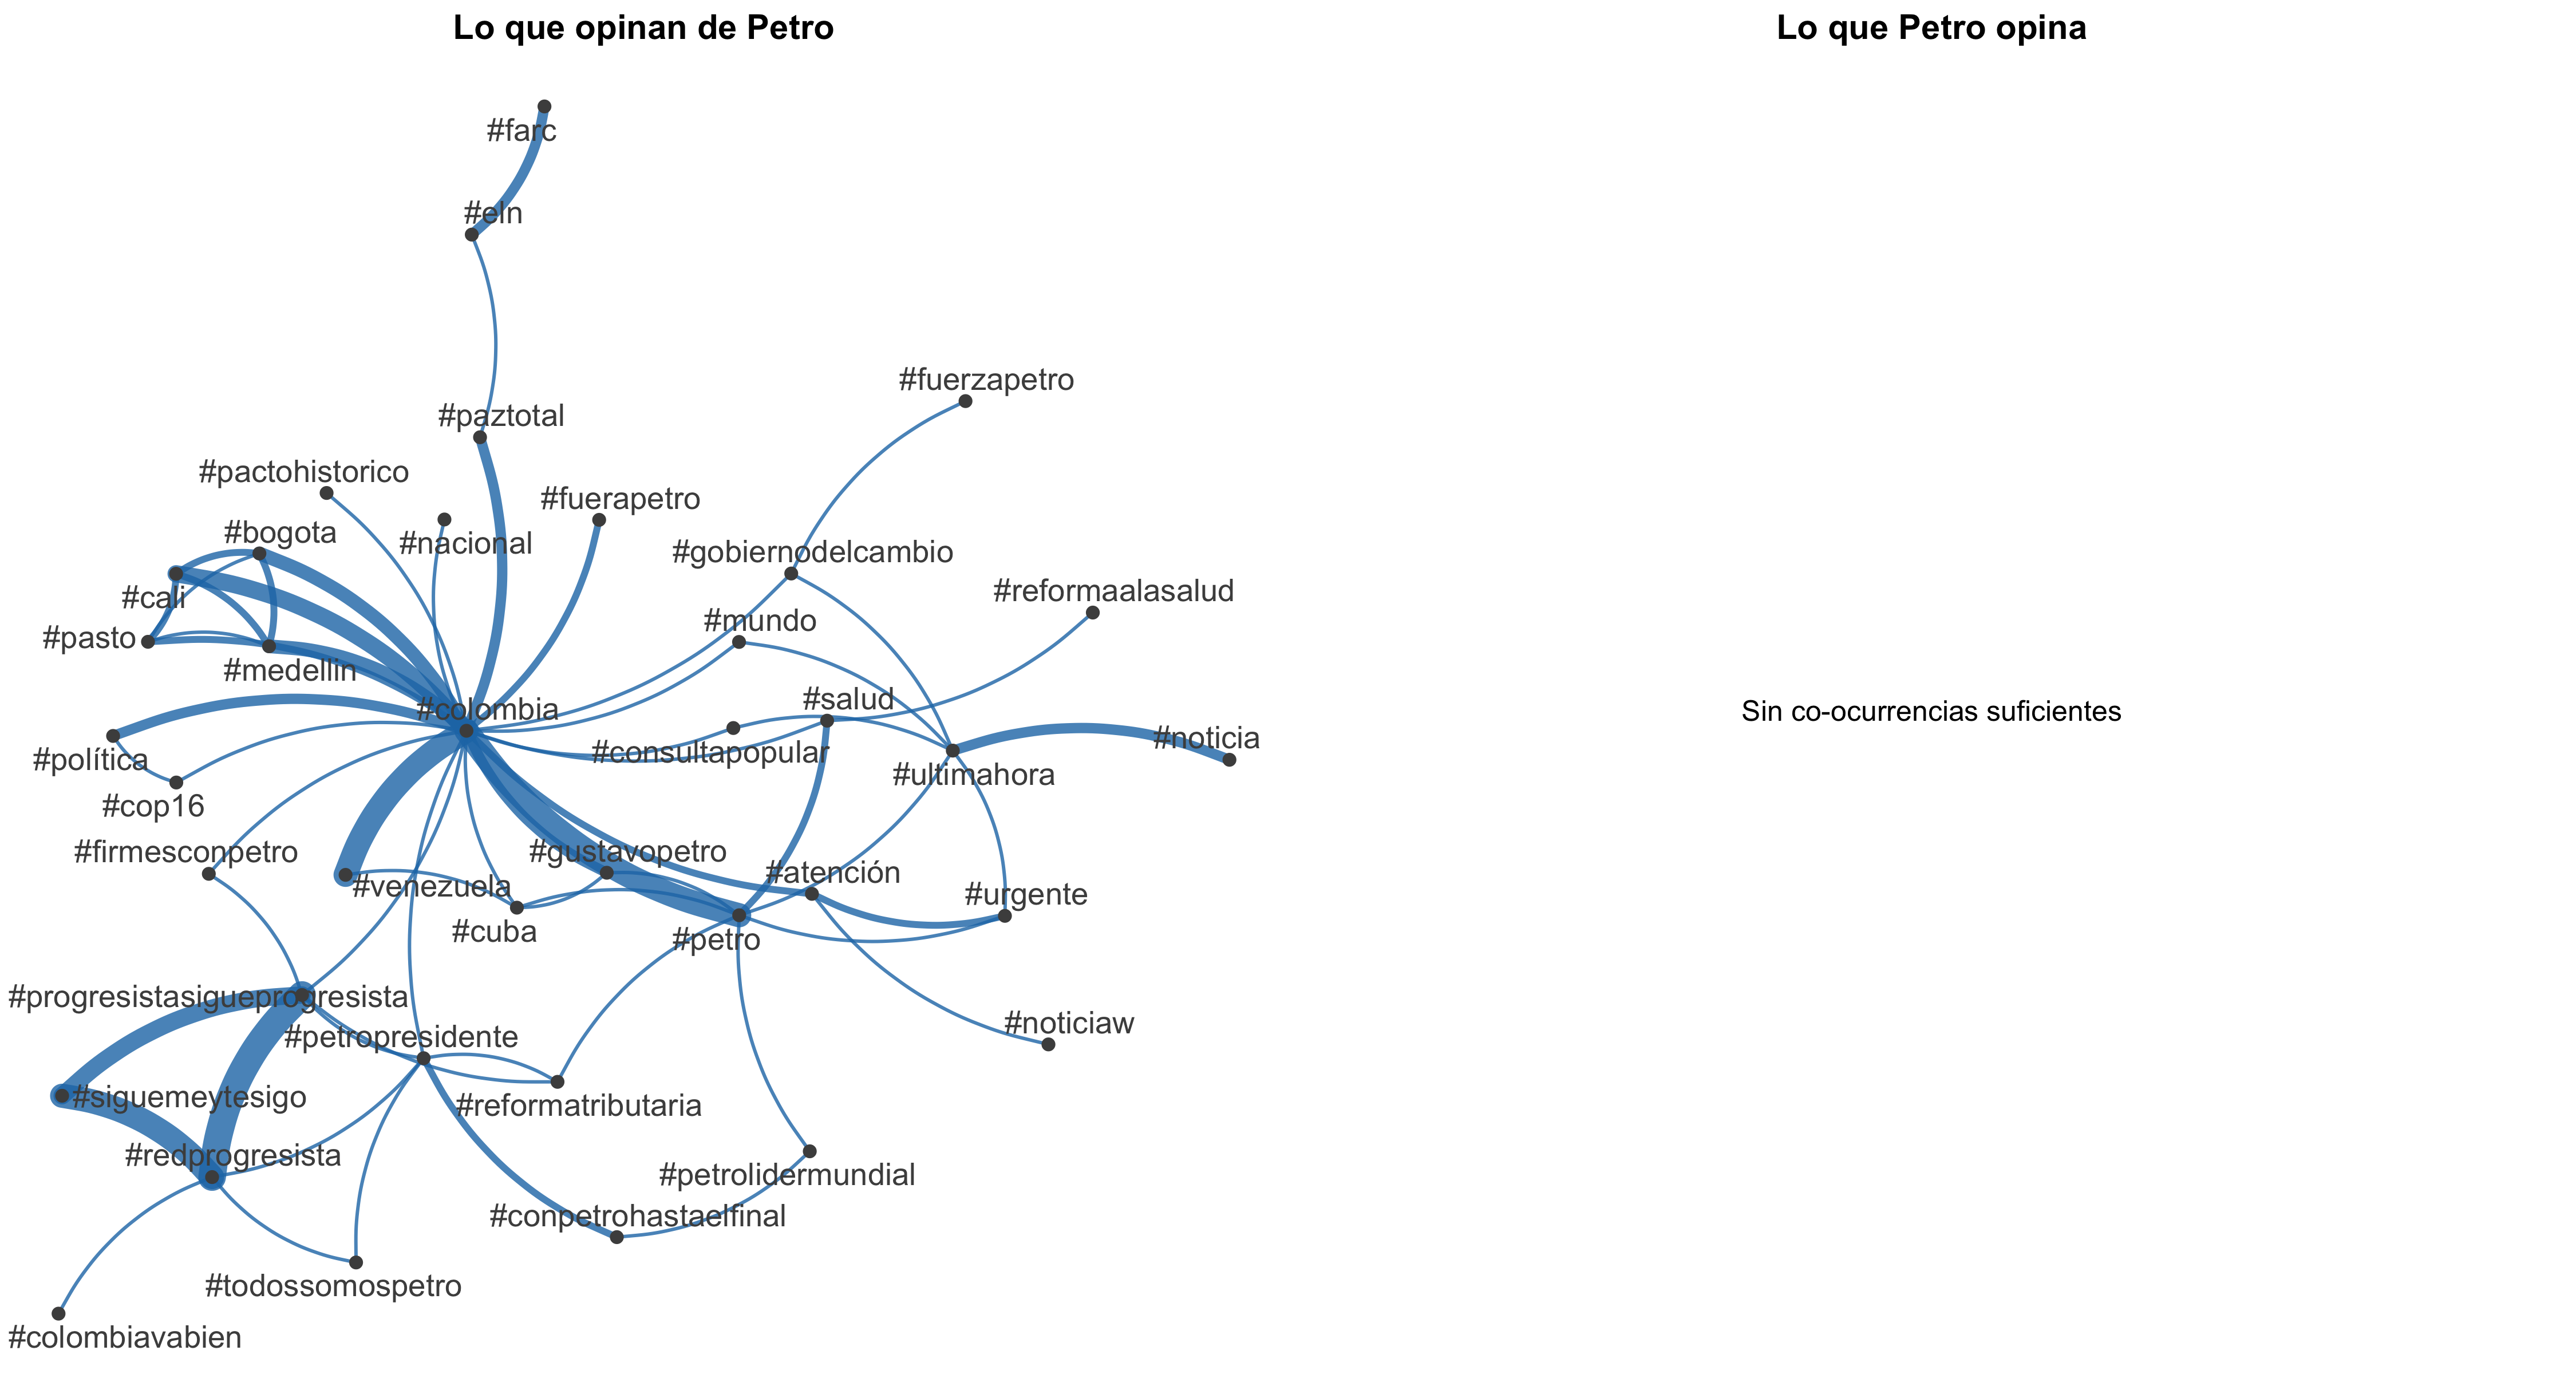
\includegraphics[width=0.95\linewidth,height=\textheight,keepaspectratio]{figures/red_hashtags_quanteda_por_corpus.png}

}

\caption{\label{fig-quanteda-hashtags-corpus}Redes de hashtags con
estilo \texttt{quanteda}, separadas por corpus.}

\end{figure}%

\begin{figure}

\centering{

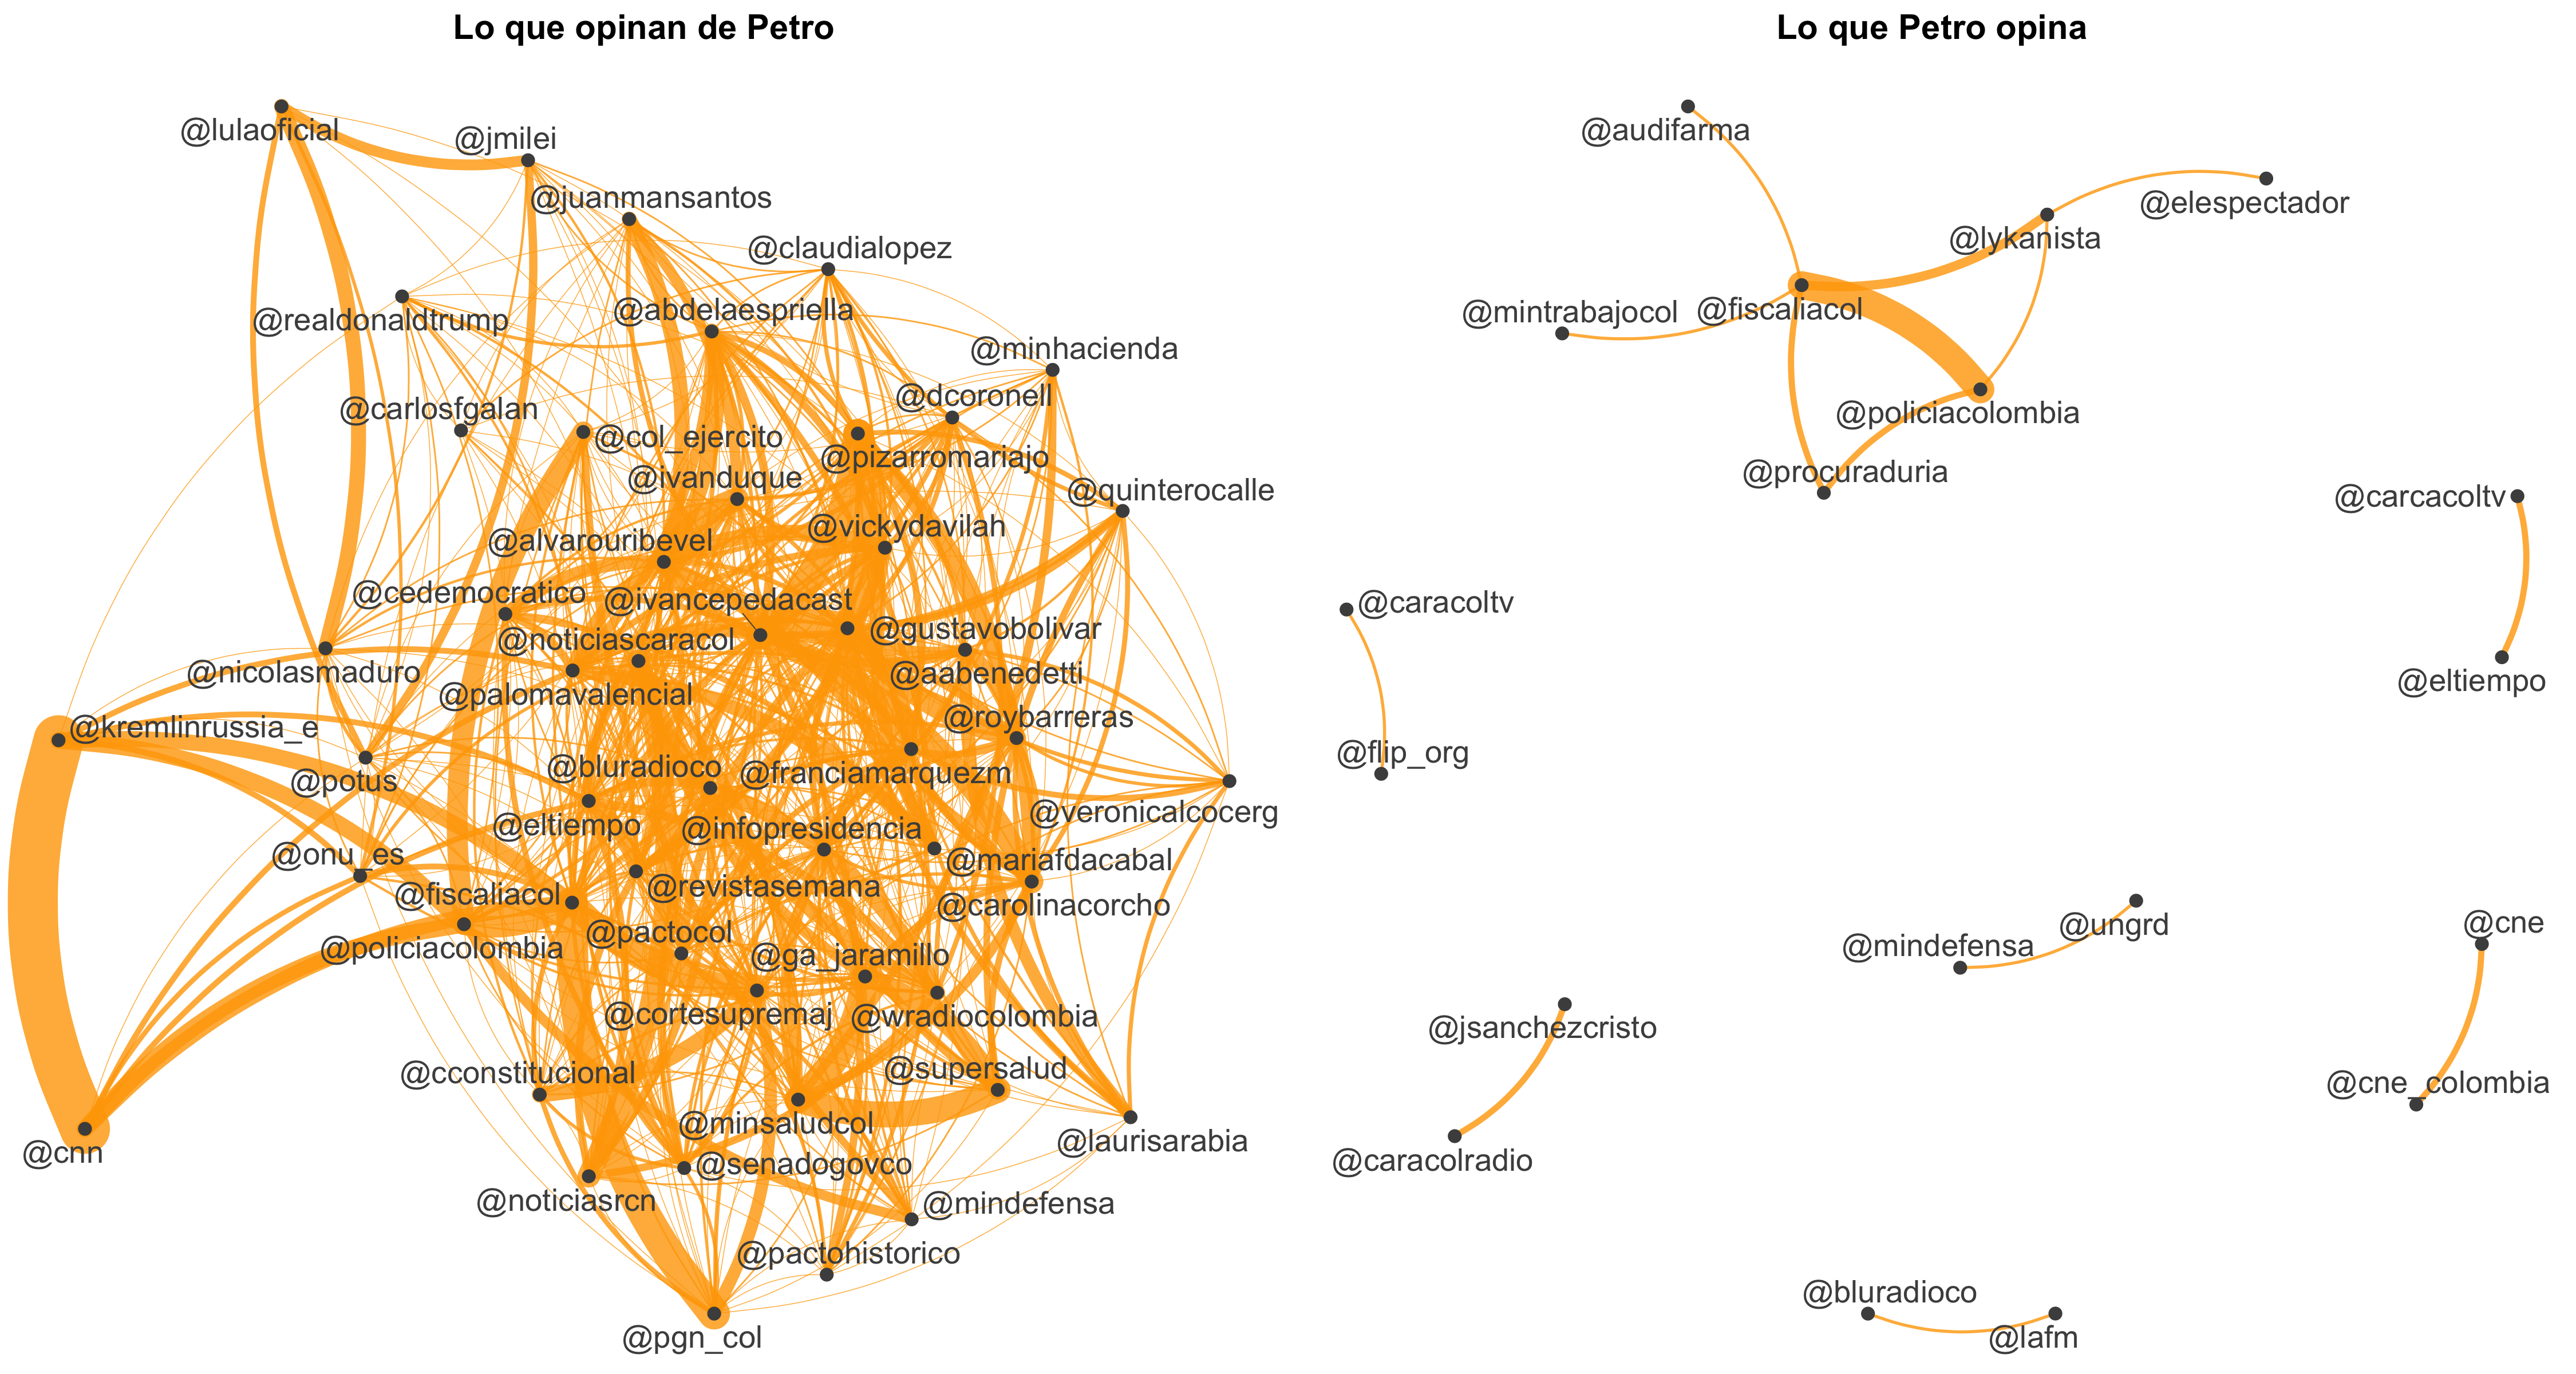
\includegraphics[width=0.95\linewidth,height=\textheight,keepaspectratio]{figures/red_menciones_quanteda_por_corpus.png}

}

\caption{\label{fig-quanteda-mentions-corpus}Redes de menciones con
estilo \texttt{quanteda}, separadas por corpus.}

\end{figure}%

La lectura de coocurrencias y keyness muestra que la palabra ``reforma''
sigue estructurando el corpus, pero ya no debe interpretarse como un
único objeto semántico. Salud, trabajo, pensiones y tributación
comparten vocabulario institucional, mientras que paz total incorpora
términos de seguridad, negociación, grupos armados, territorios y
capacidad estatal. Esta distinción corrige una limitación del análisis
inicial, donde el debate reformista podía quedar agrupado de manera
demasiado amplia. La clasificación temática con supervisión débil reduce
parcialmente la categoría \texttt{otros} bajo umbral de confianza, de
modo que la reclasificación se usa para sensibilidad descriptiva y no
para afirmar una verdad sustantiva definitiva.

\begin{figure}

\centering{

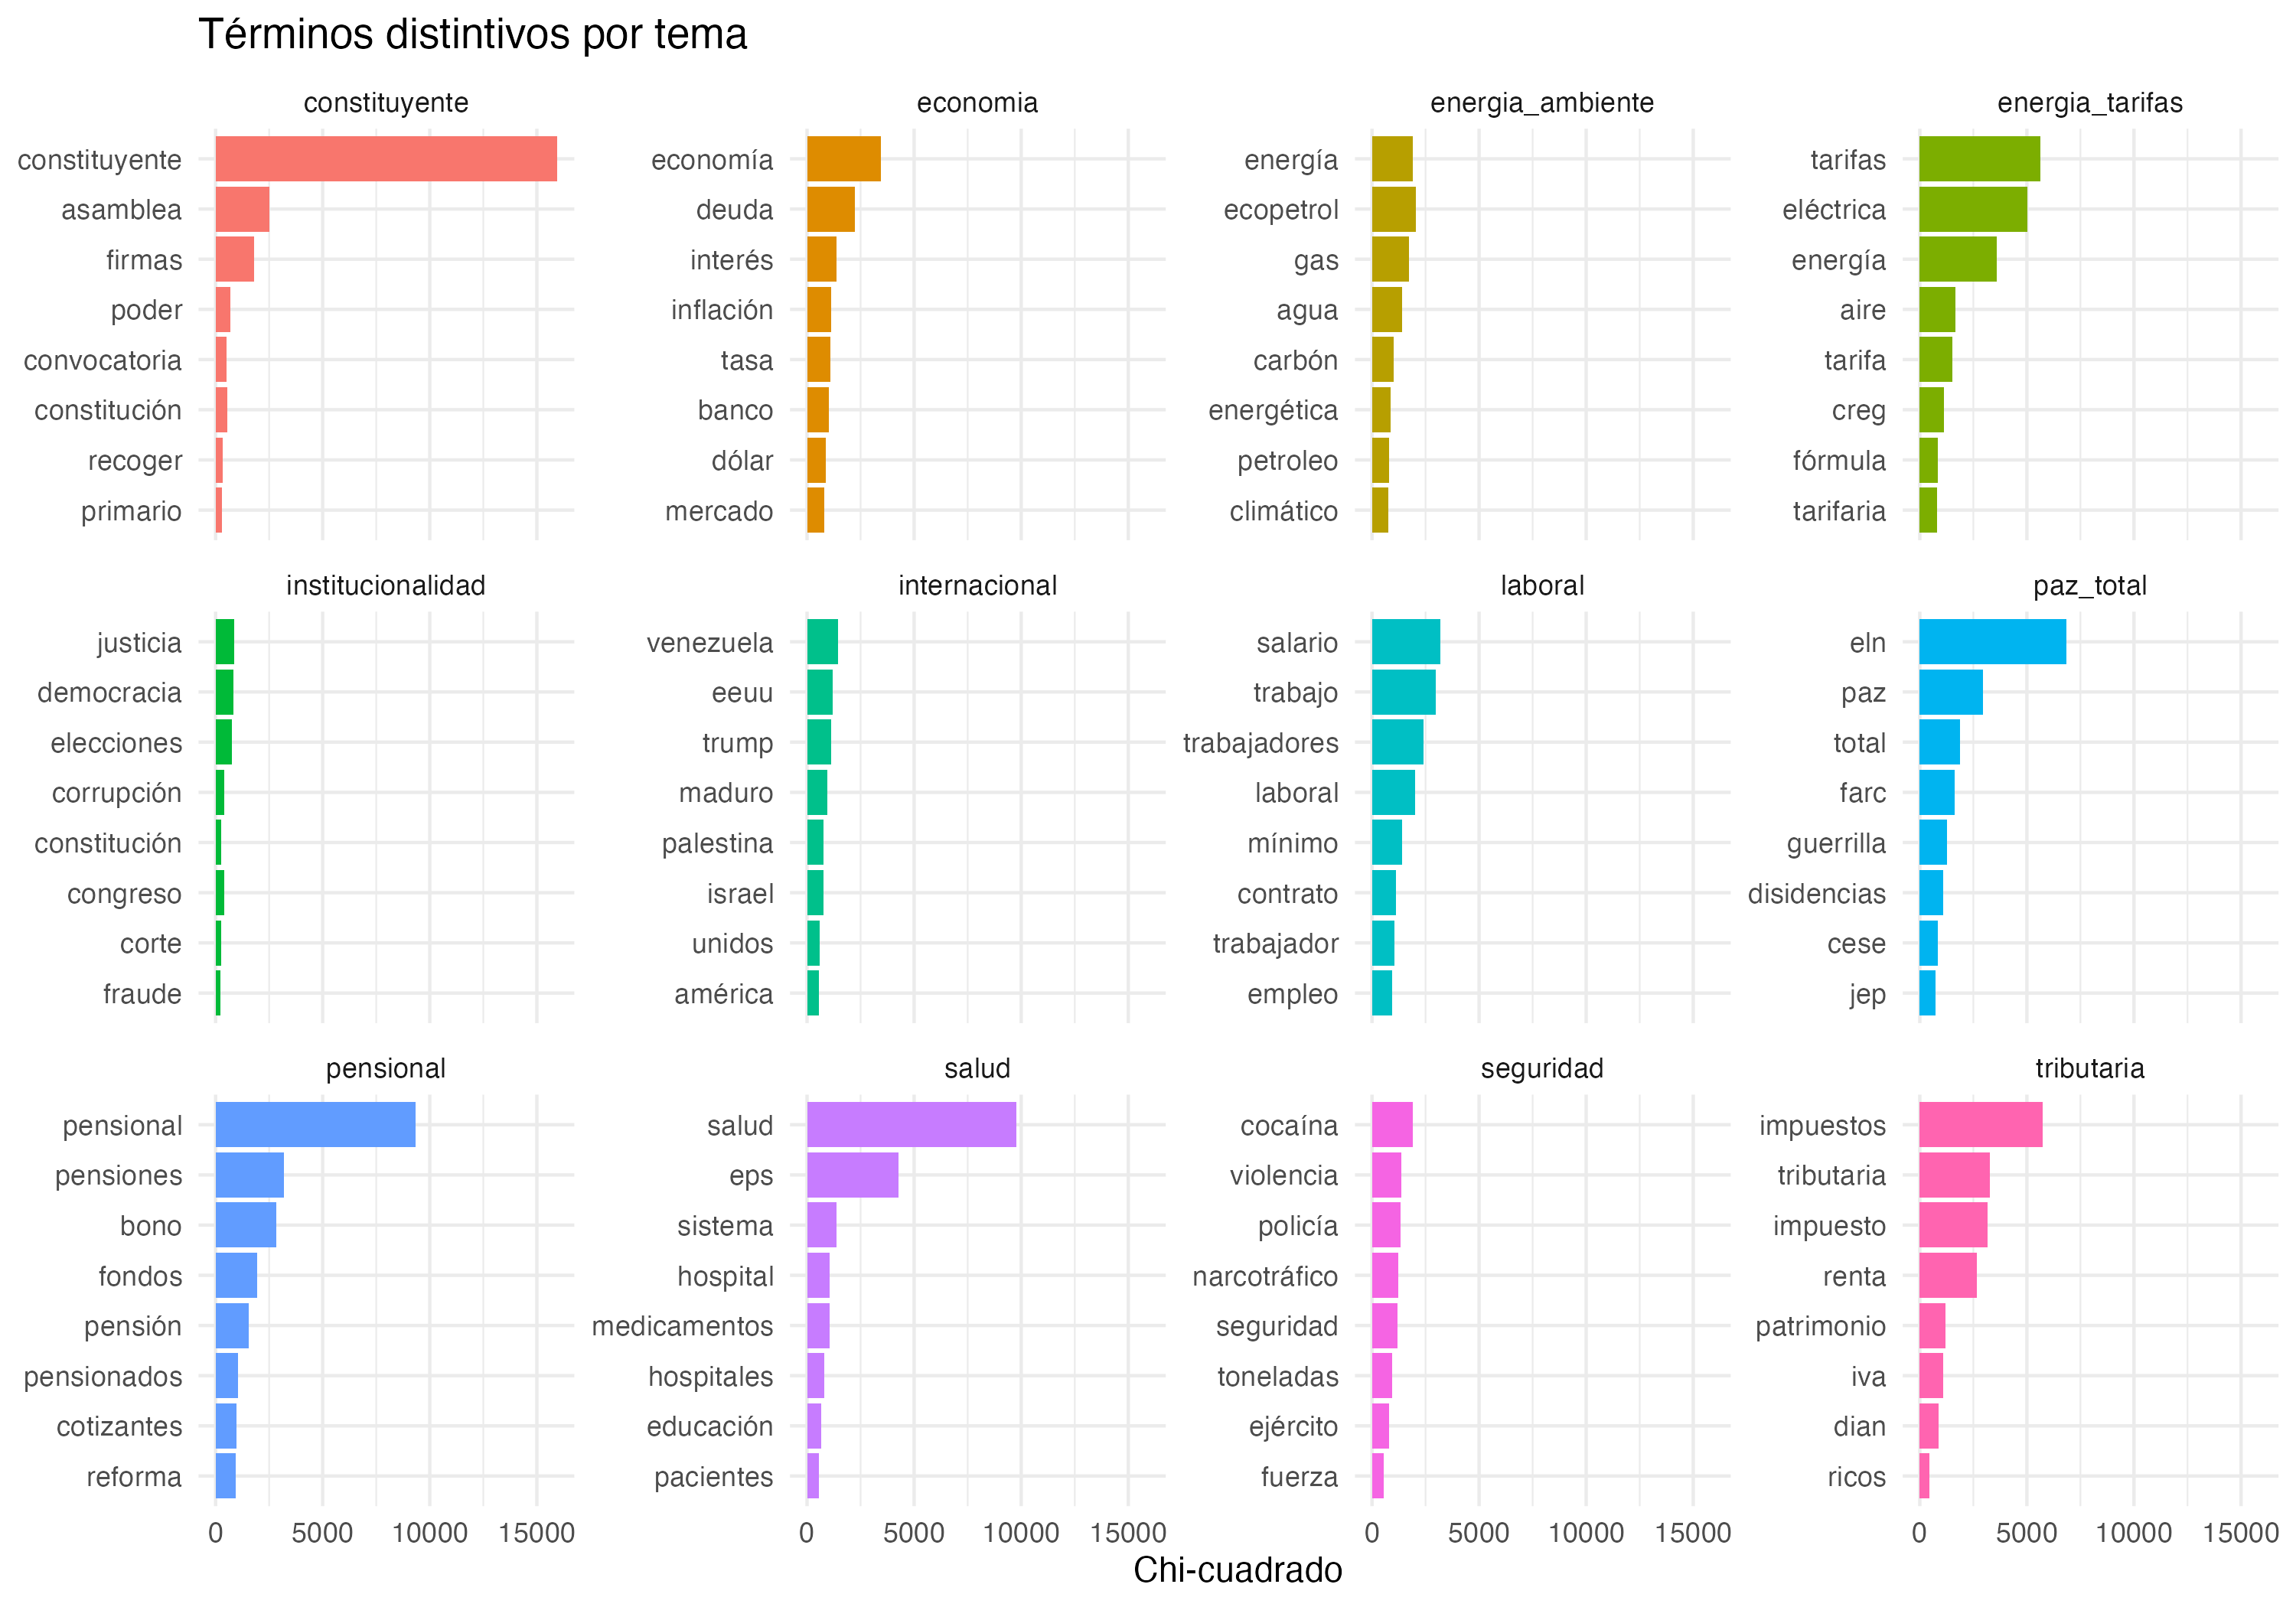
\includegraphics[width=0.9\linewidth,height=\textheight,keepaspectratio]{figures/keyness_reformas.png}

}

\caption{\label{fig-keyness}Términos distintivos por tema de reforma y
política pública.}

\end{figure}%

\begin{figure}

\centering{

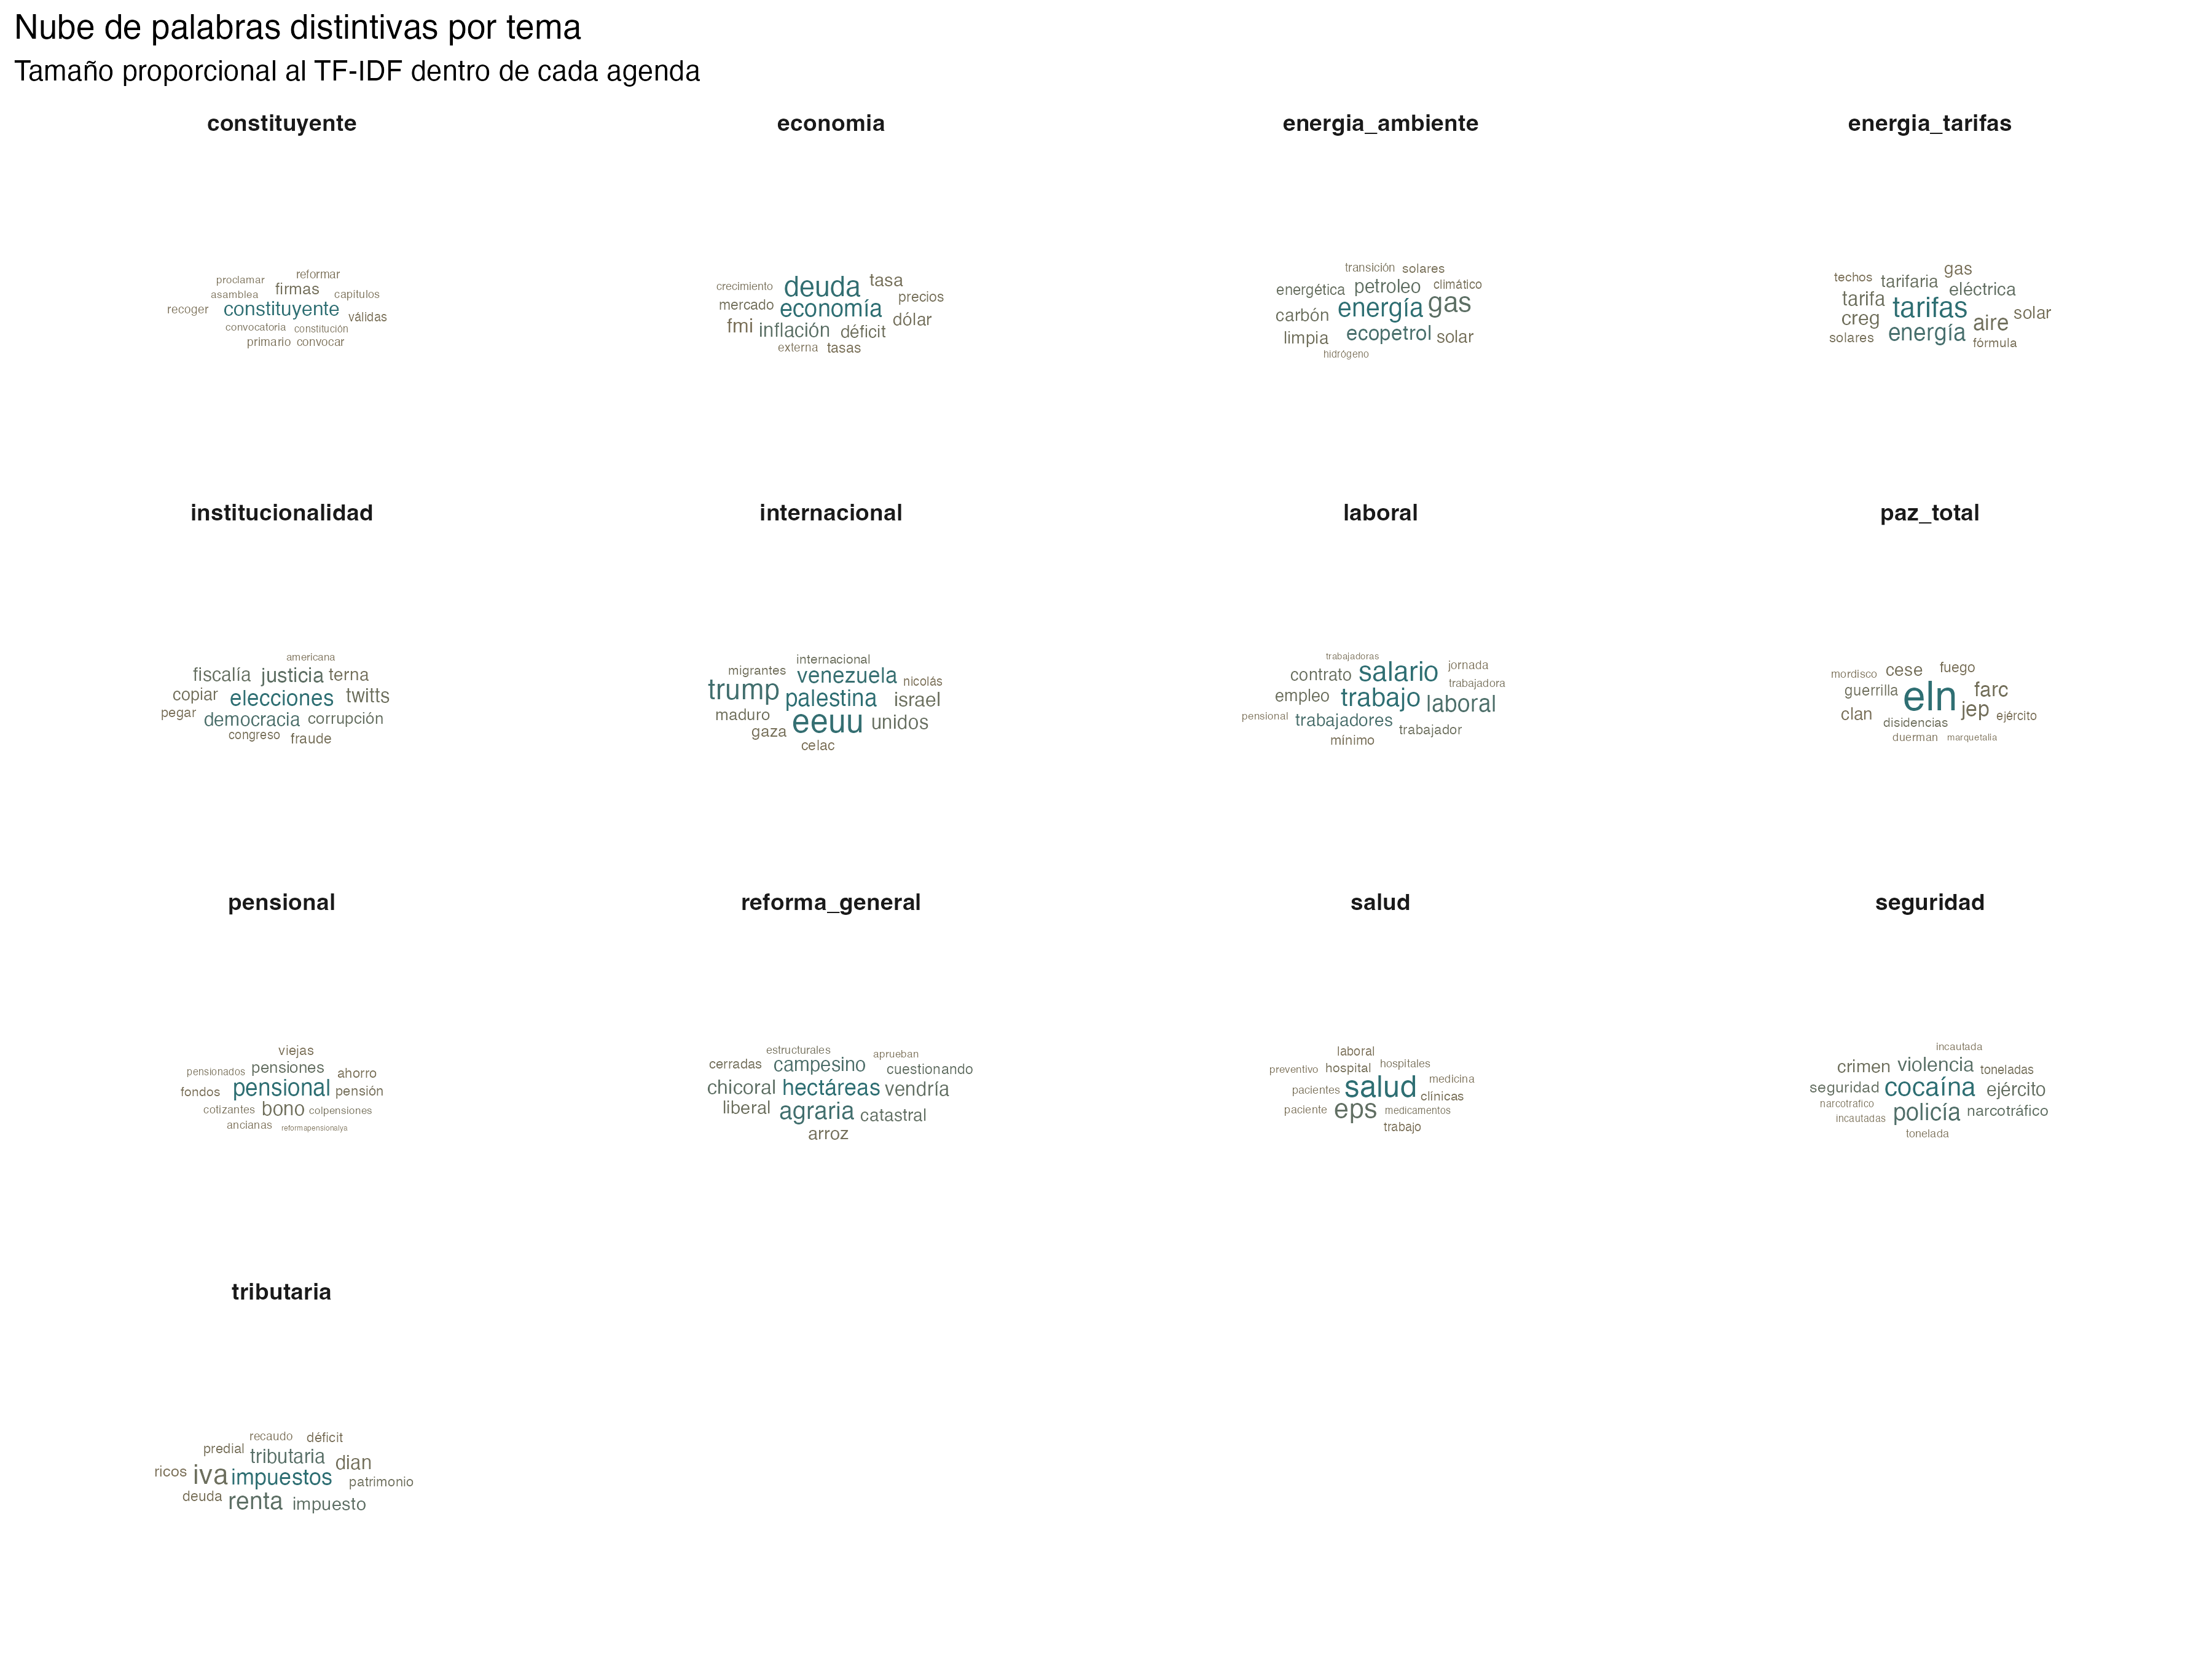
\includegraphics[width=0.9\linewidth,height=\textheight,keepaspectratio]{figures/wordcloud_temas_tfidf.png}

}

\caption{\label{fig-theme-cloud}Nube de palabras distintivas por tema,
ponderadas por TF-IDF.}

\end{figure}%

\begin{figure}

\centering{

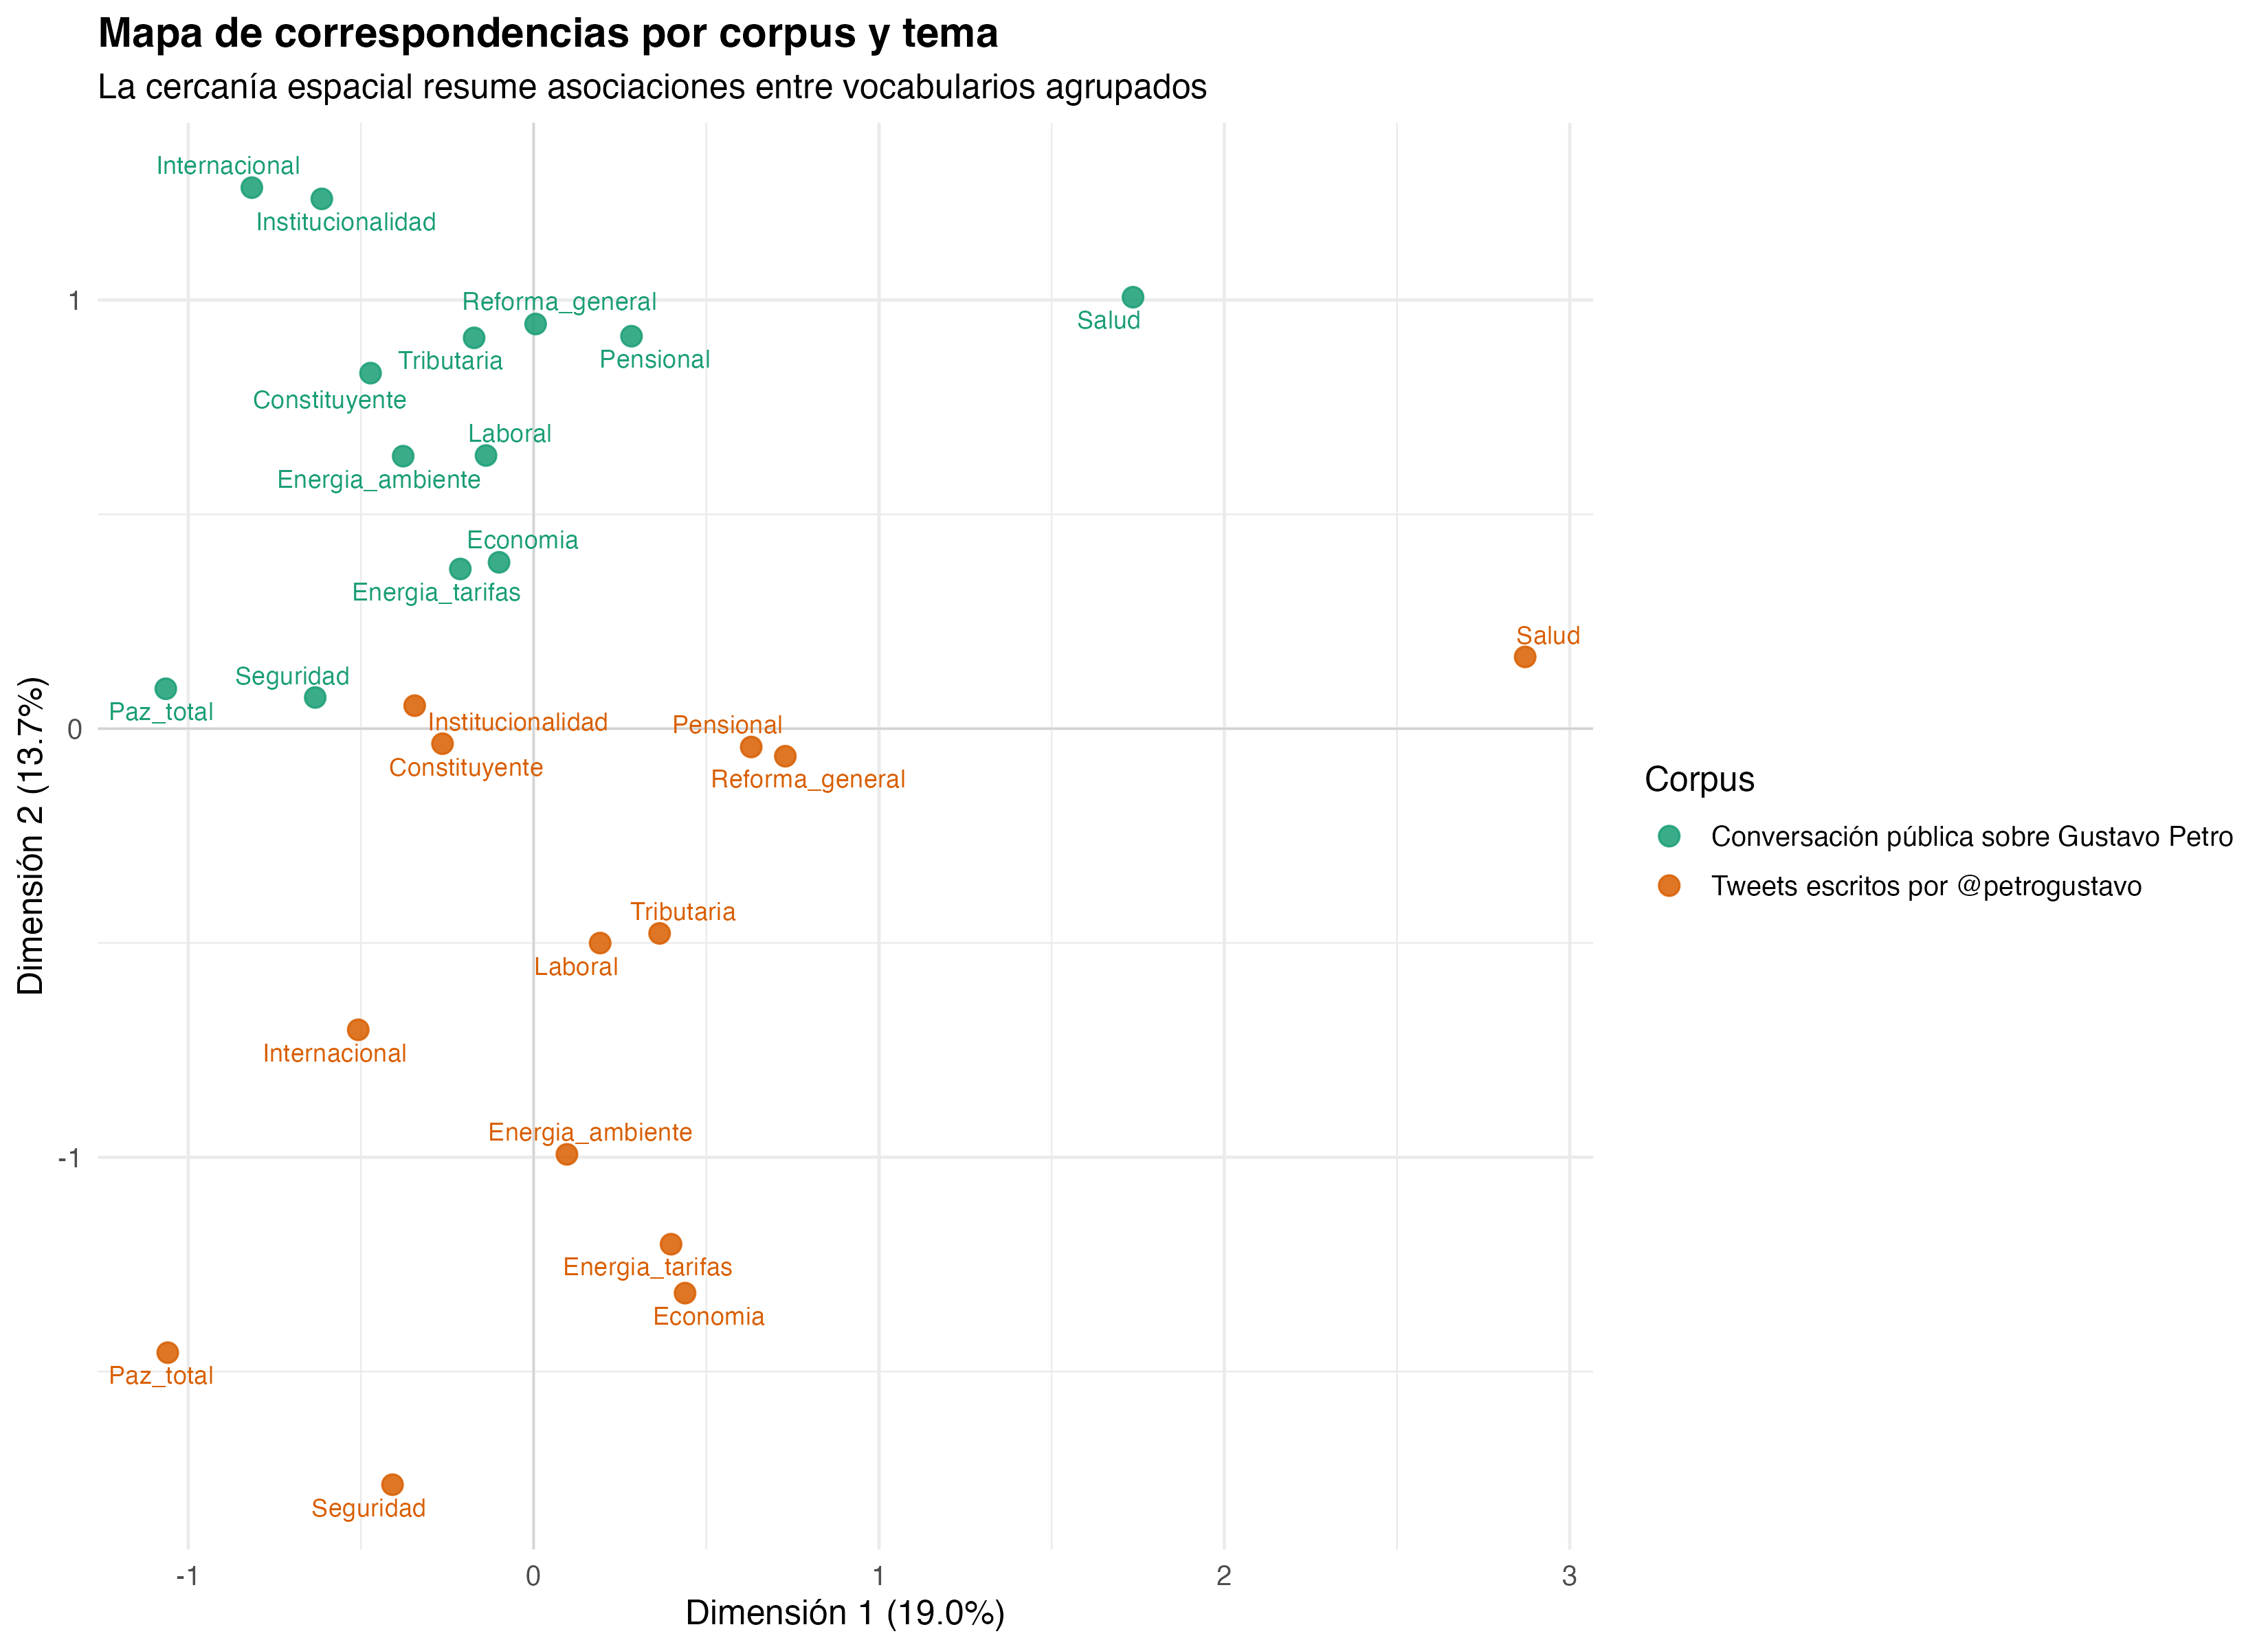
\includegraphics[width=0.85\linewidth,height=\textheight,keepaspectratio]{figures/ca_temas_quanteda.png}

}

\caption{\label{fig-ca-themes}Análisis de correspondencias de temas y
términos con \texttt{quanteda}.}

\end{figure}%

\begin{figure}

\centering{

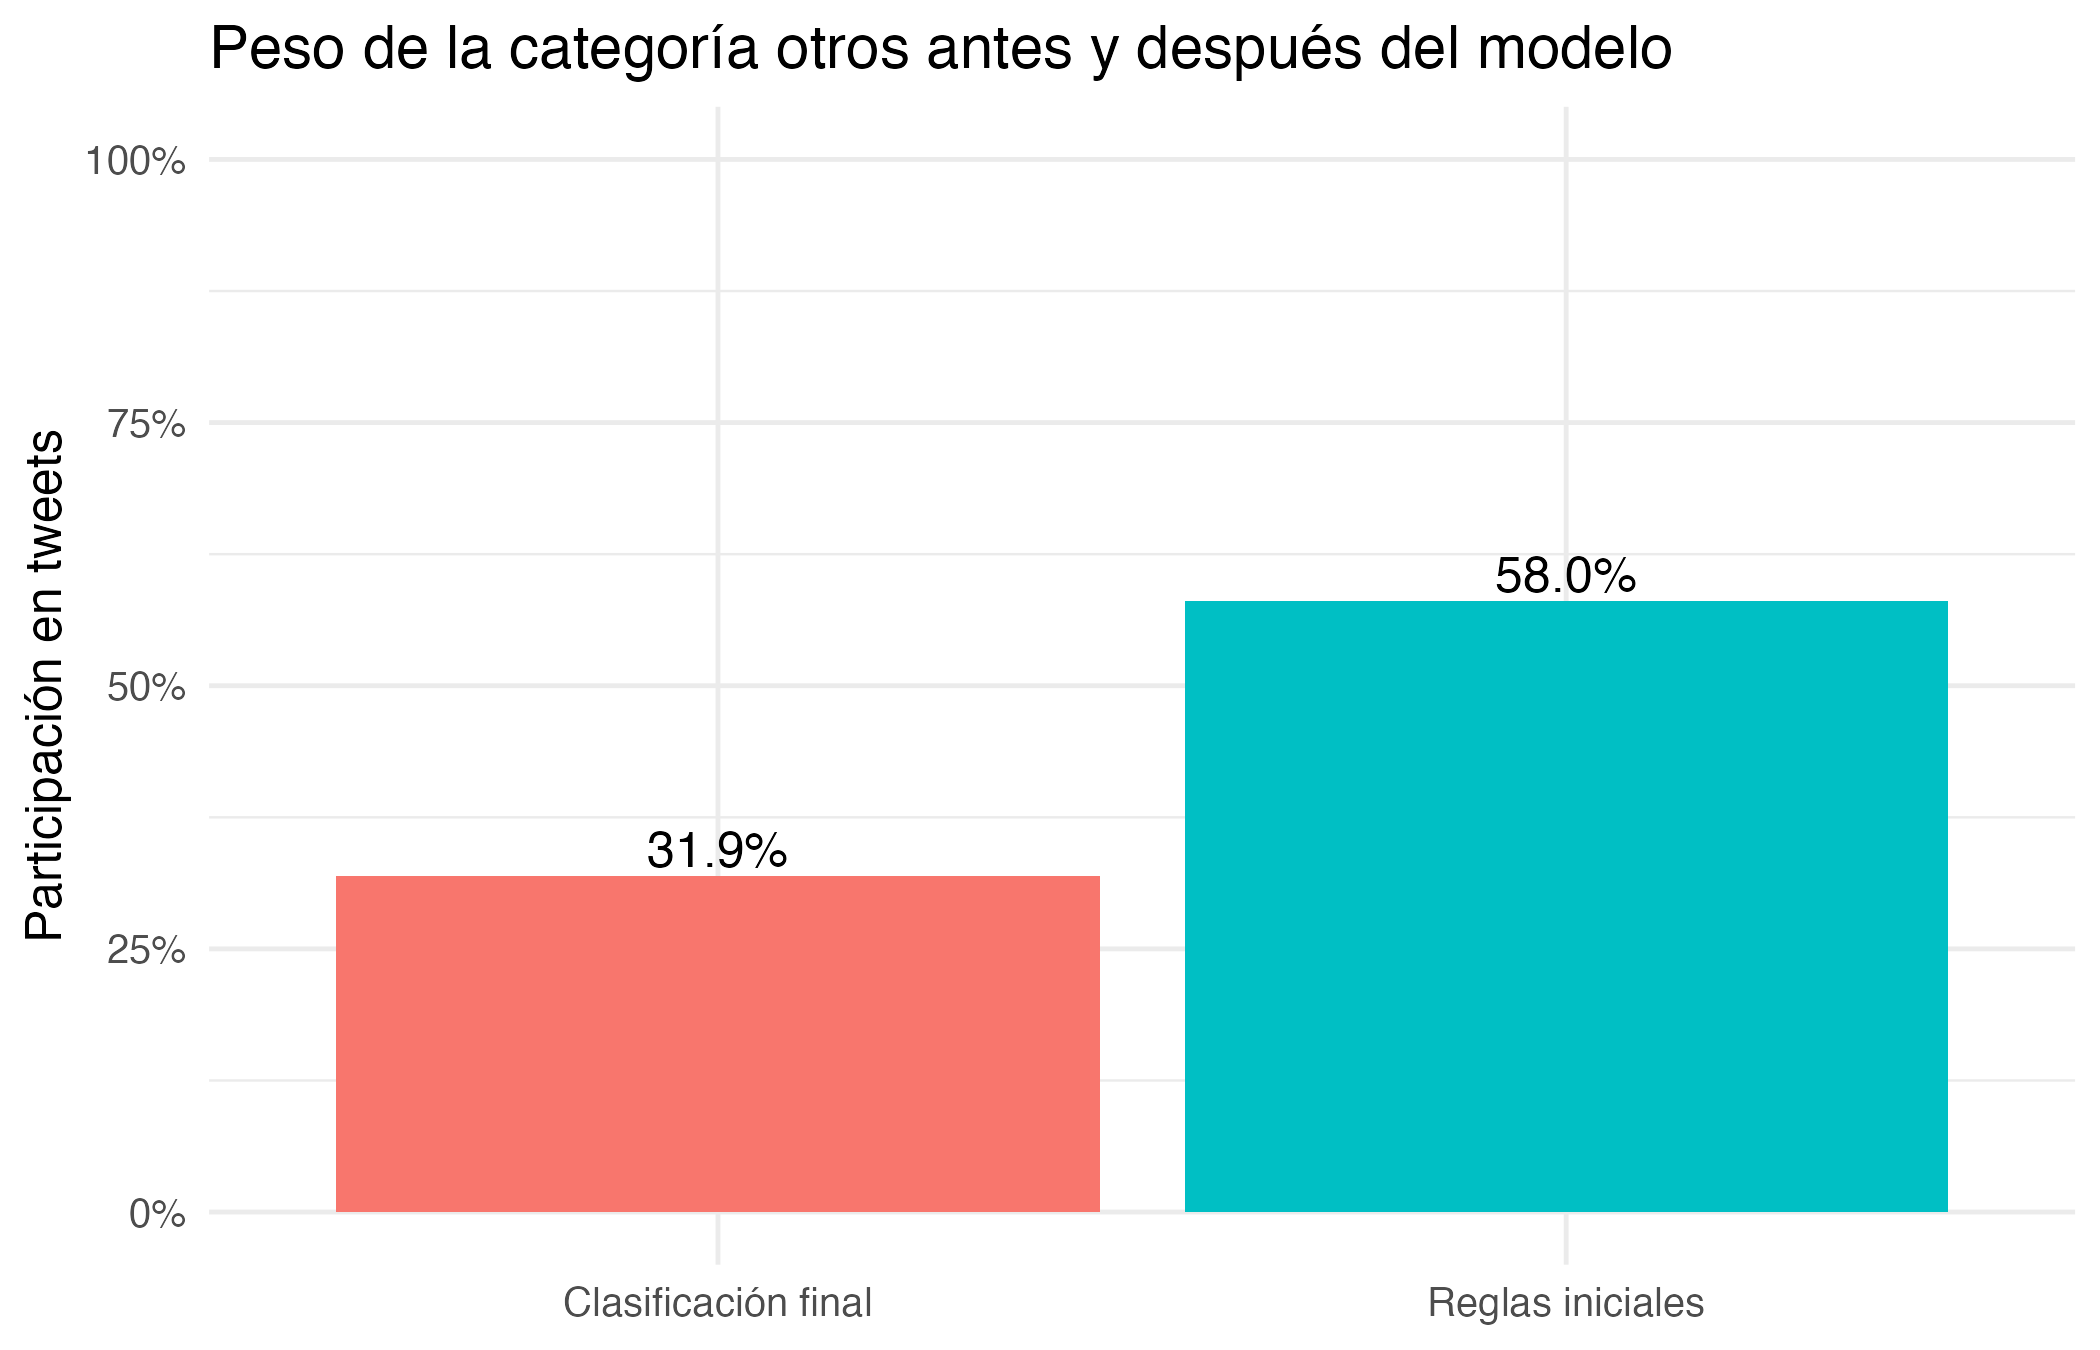
\includegraphics[width=0.75\linewidth,height=\textheight,keepaspectratio]{figures/ml_reduccion_otros.png}

}

\caption{\label{fig-ml-other}Reducción conservadora de la categoría
otros después de clasificación temática.}

\end{figure}%

Los tópicos estimados deben leerse como exploratorios. Twitter/X combina
textos cortos, ironía, hashtags, citas, enlaces y confrontación
política, lo que puede reducir la coherencia semántica de modelos
latentes. Por eso, la interpretación combina STM con keyness, redes,
Wordfish, entidades de spaCy y evidencia temporal. Esta triangulación
preserva el enfoque del paper original y reduce el riesgo de
sobrerrepresentar un solo algoritmo.

\begin{figure}

\centering{

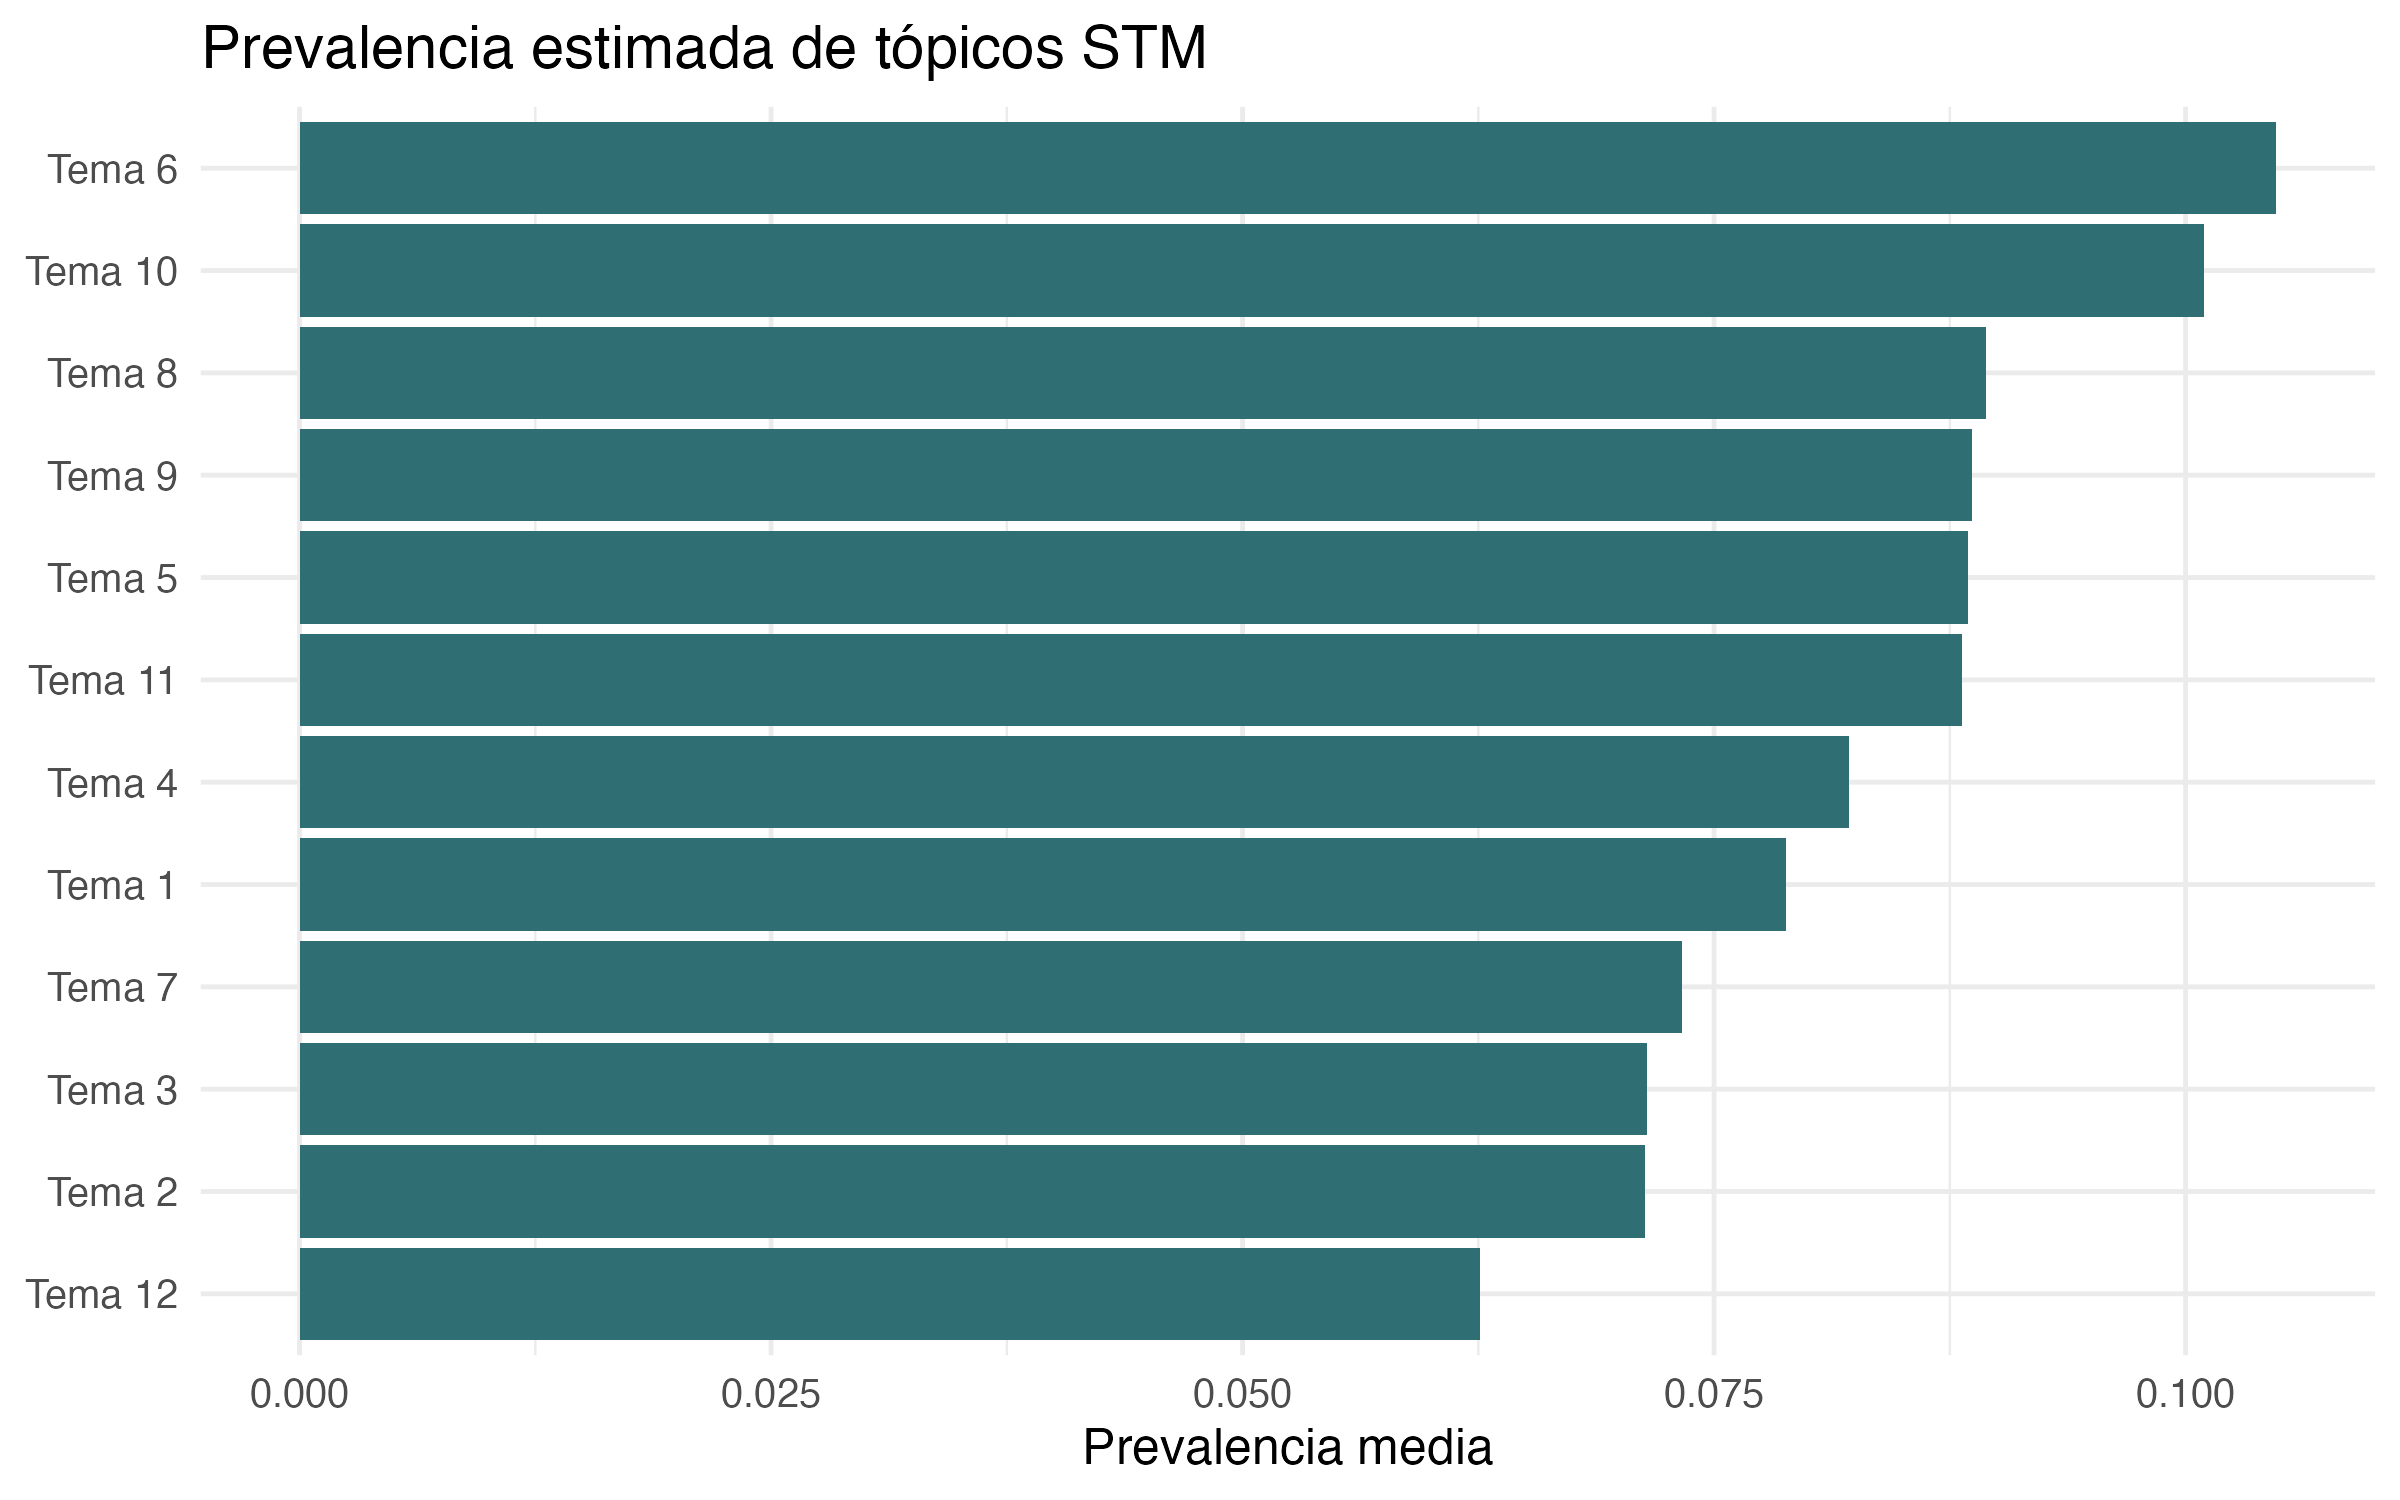
\includegraphics[width=0.8\linewidth,height=\textheight,keepaspectratio]{figures/stm_topicos_reformas.png}

}

\caption{\label{fig-stm}Prevalencia estimada de tópicos STM.}

\end{figure}%

\begin{figure}

\centering{

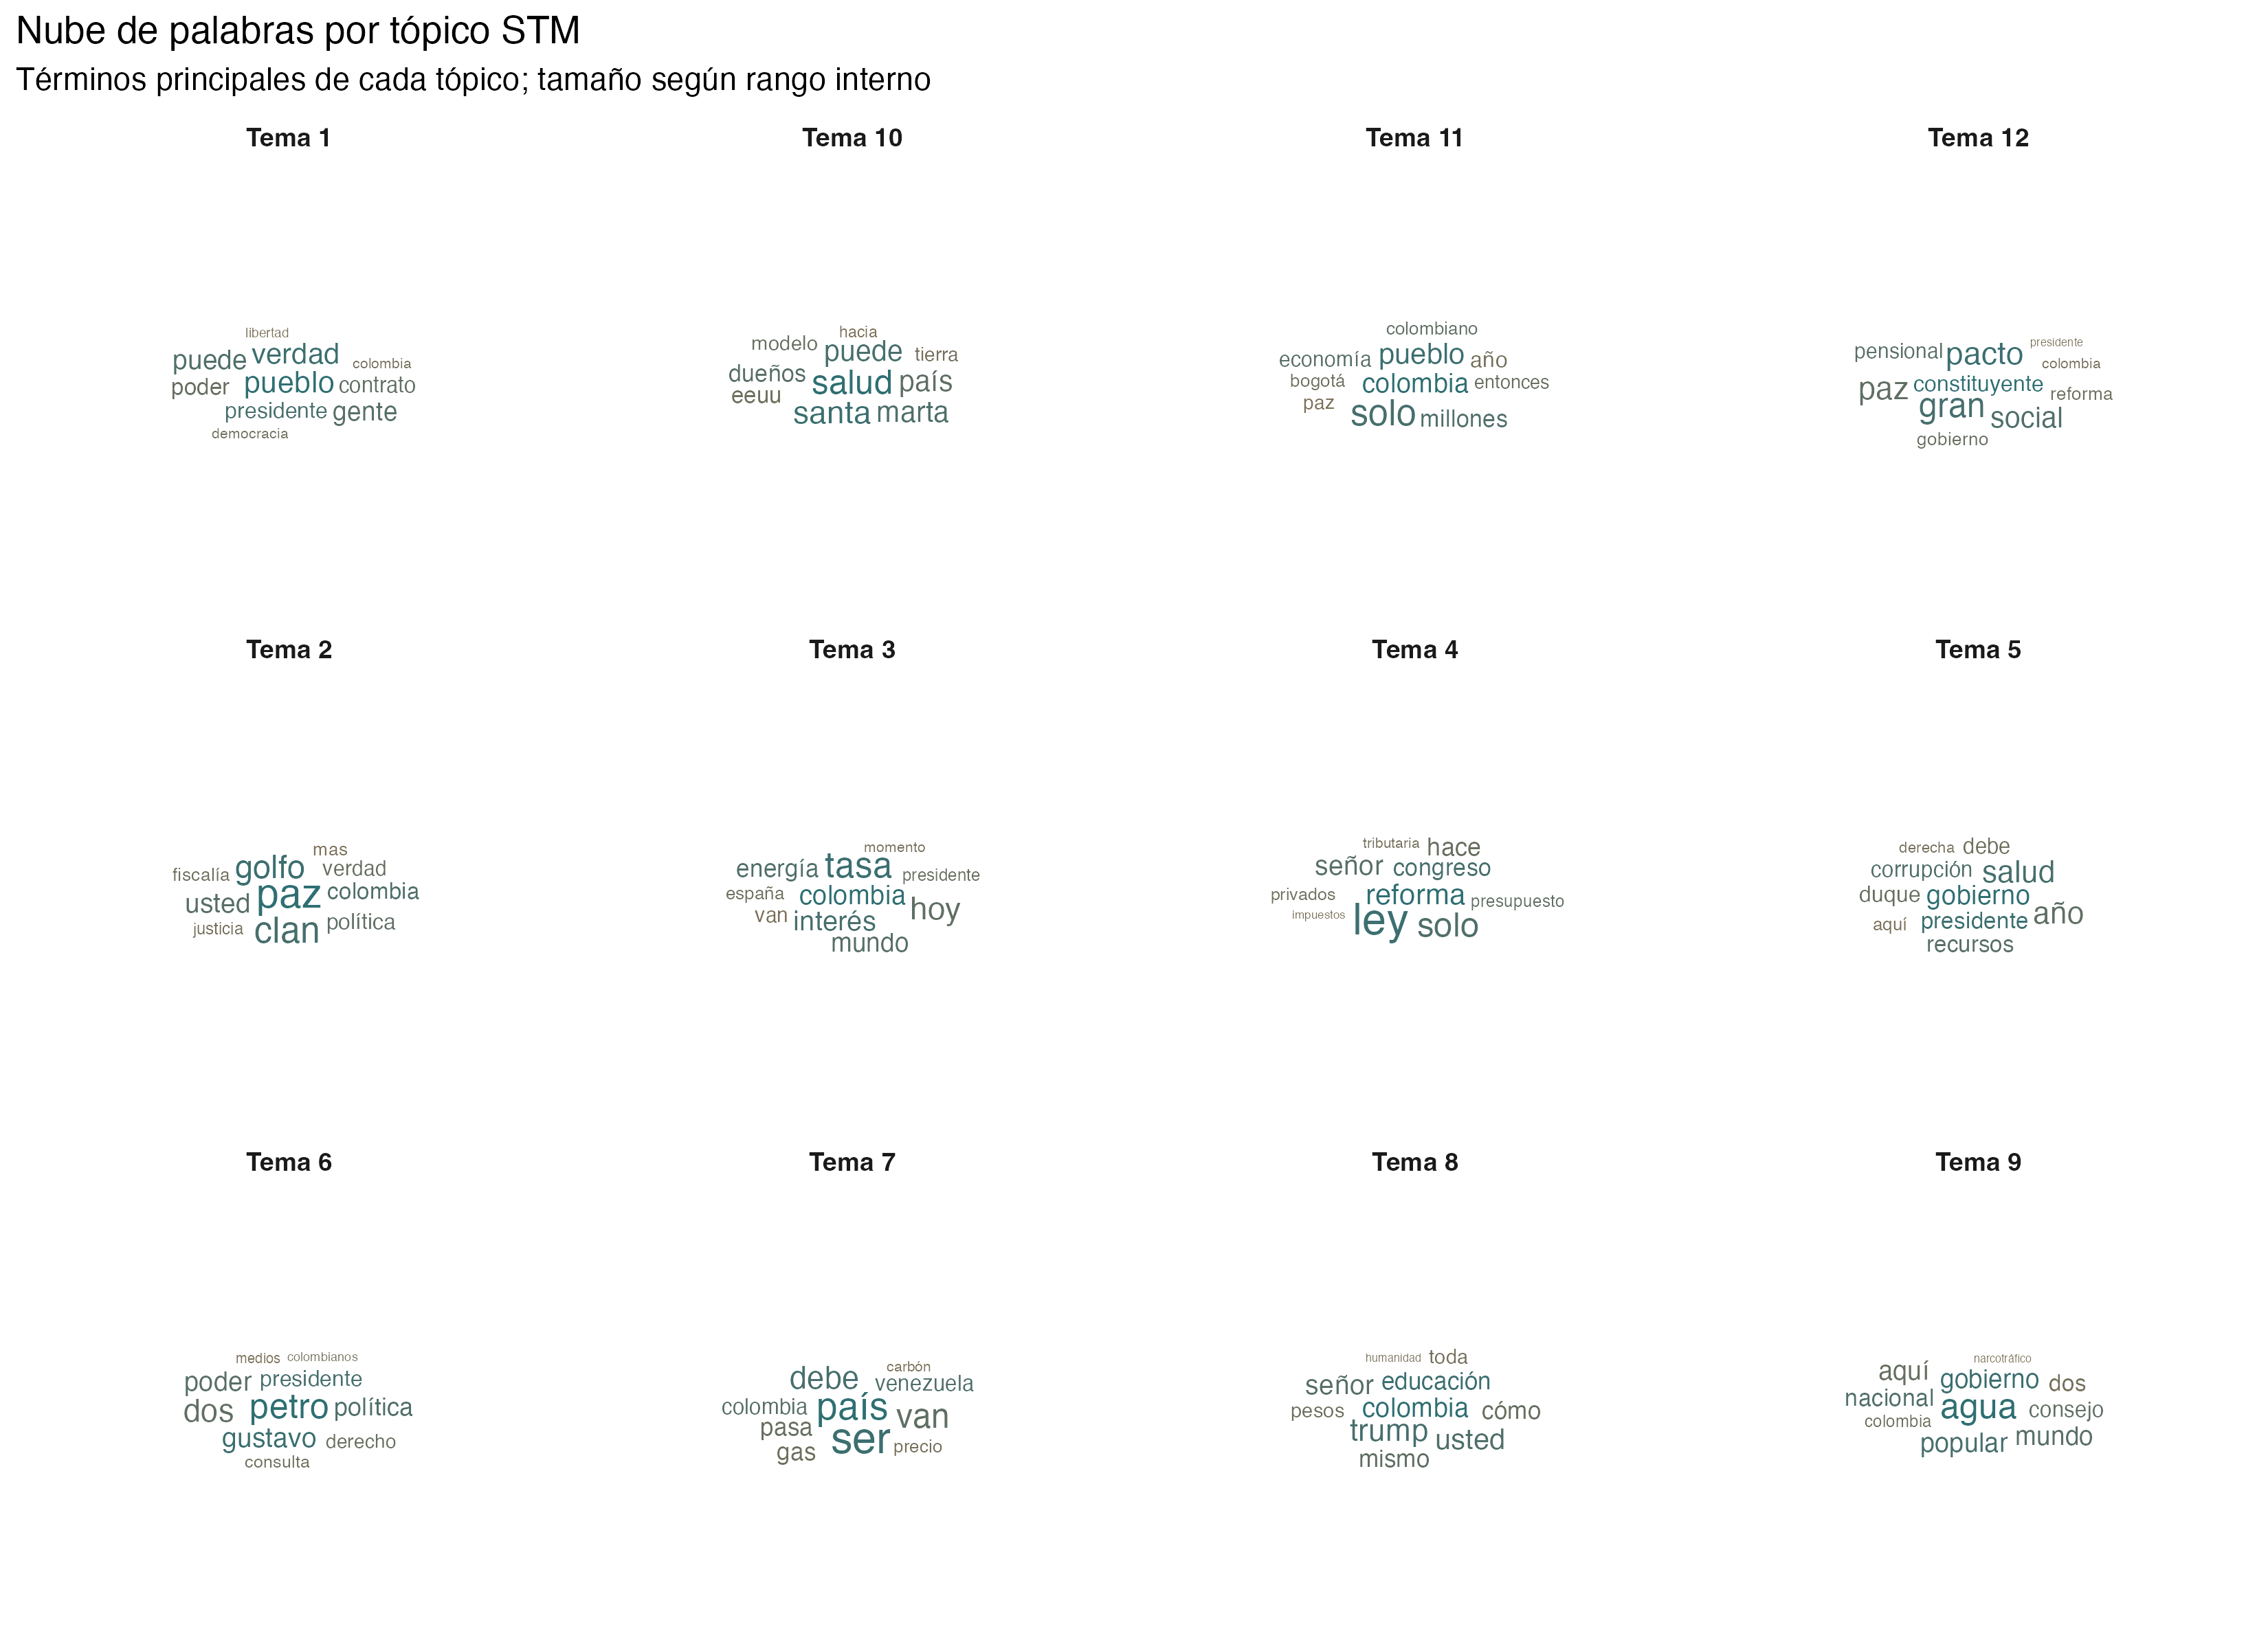
\includegraphics[width=0.9\linewidth,height=\textheight,keepaspectratio]{figures/wordcloud_topicos_stm.png}

}

\caption{\label{fig-topic-cloud}Nube de palabras por tópico STM.}

\end{figure}%

Los resultados sentimentales mantienen la intuición original: la
conversación sobre Petro es emocionalmente heterogénea. La nueva
separación muestra además que esa conversación no debe confundirse con
el tono presidencial directo. Confianza, miedo, ira, tristeza y
anticipación aparecen como dimensiones relevantes, pero su significado
depende del tema, del momento y del corpus. La versión mejorada agrega
series diarias, polaridad, agregación sentométrica, fechas pico e Índice
de Presión Informacional para comparar tono e intensidad con variables
financieras.

\begin{figure}

\centering{

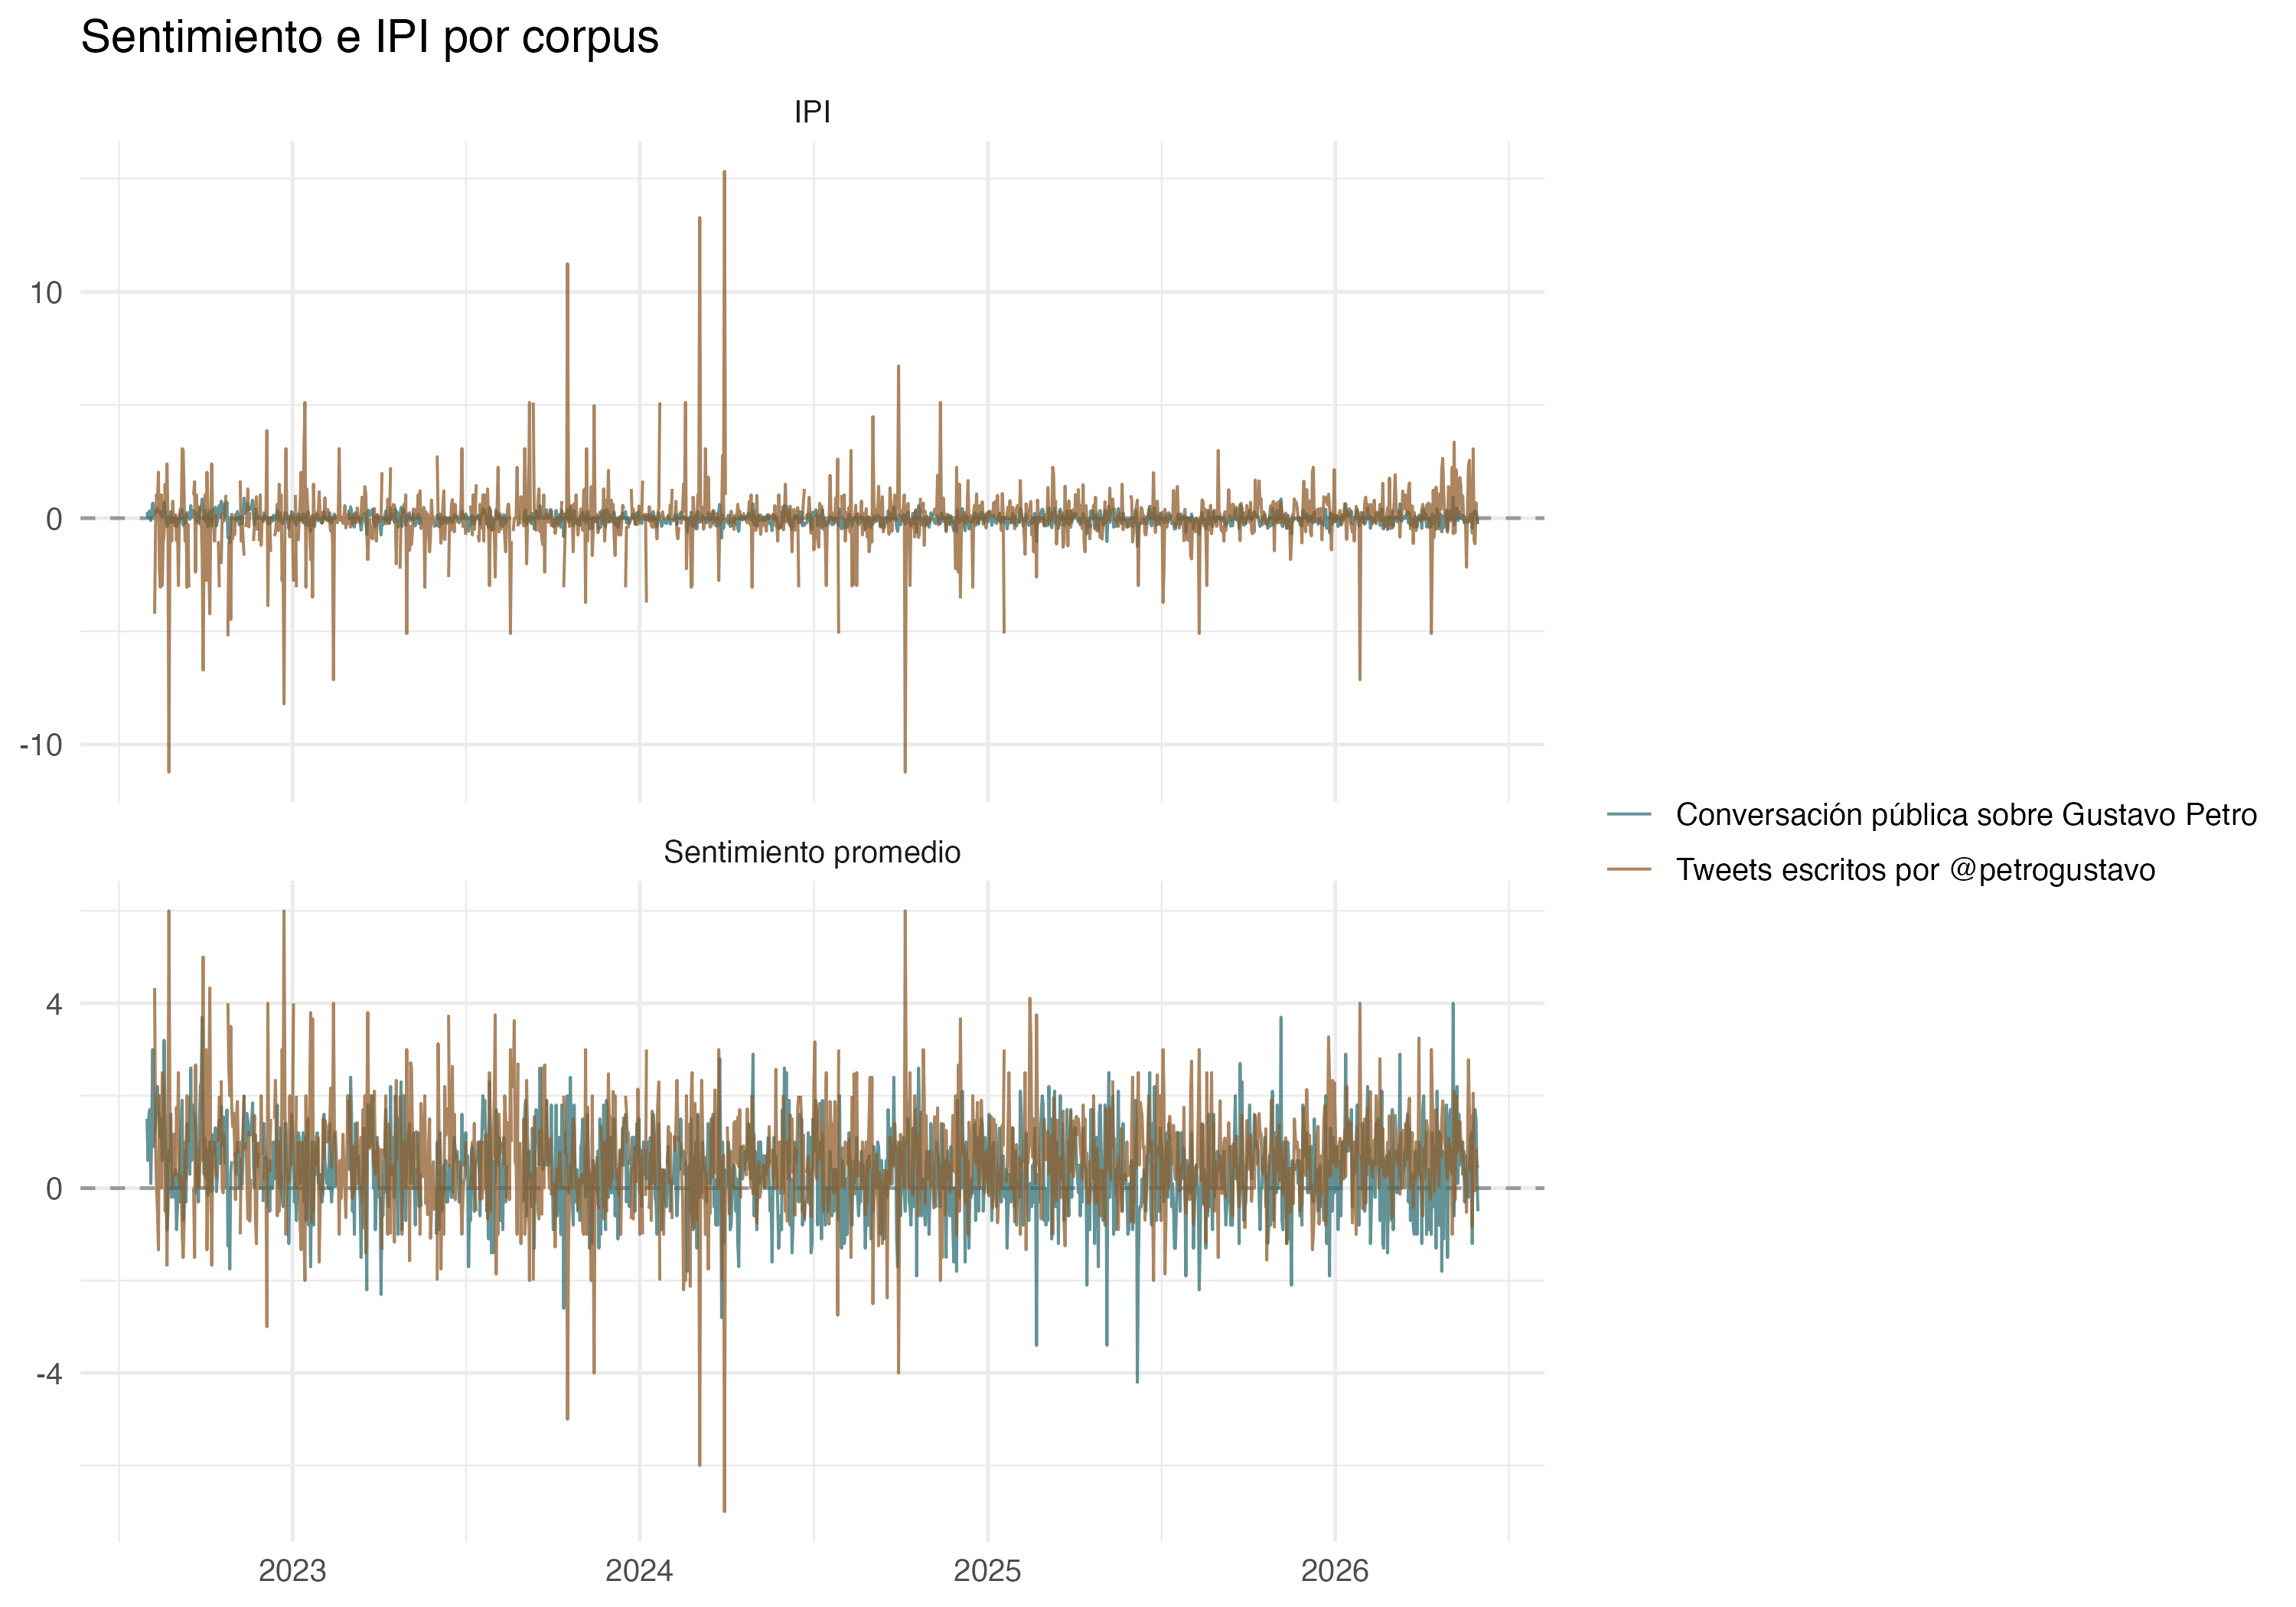
\includegraphics[width=0.9\linewidth,height=\textheight,keepaspectratio]{figures/comparacion_corpus_sentimiento.png}

}

\caption{\label{fig-corpus-sentiment}Sentimiento promedio e Índice de
Presión Informacional por corpus.}

\end{figure}%

\begin{figure}

\centering{

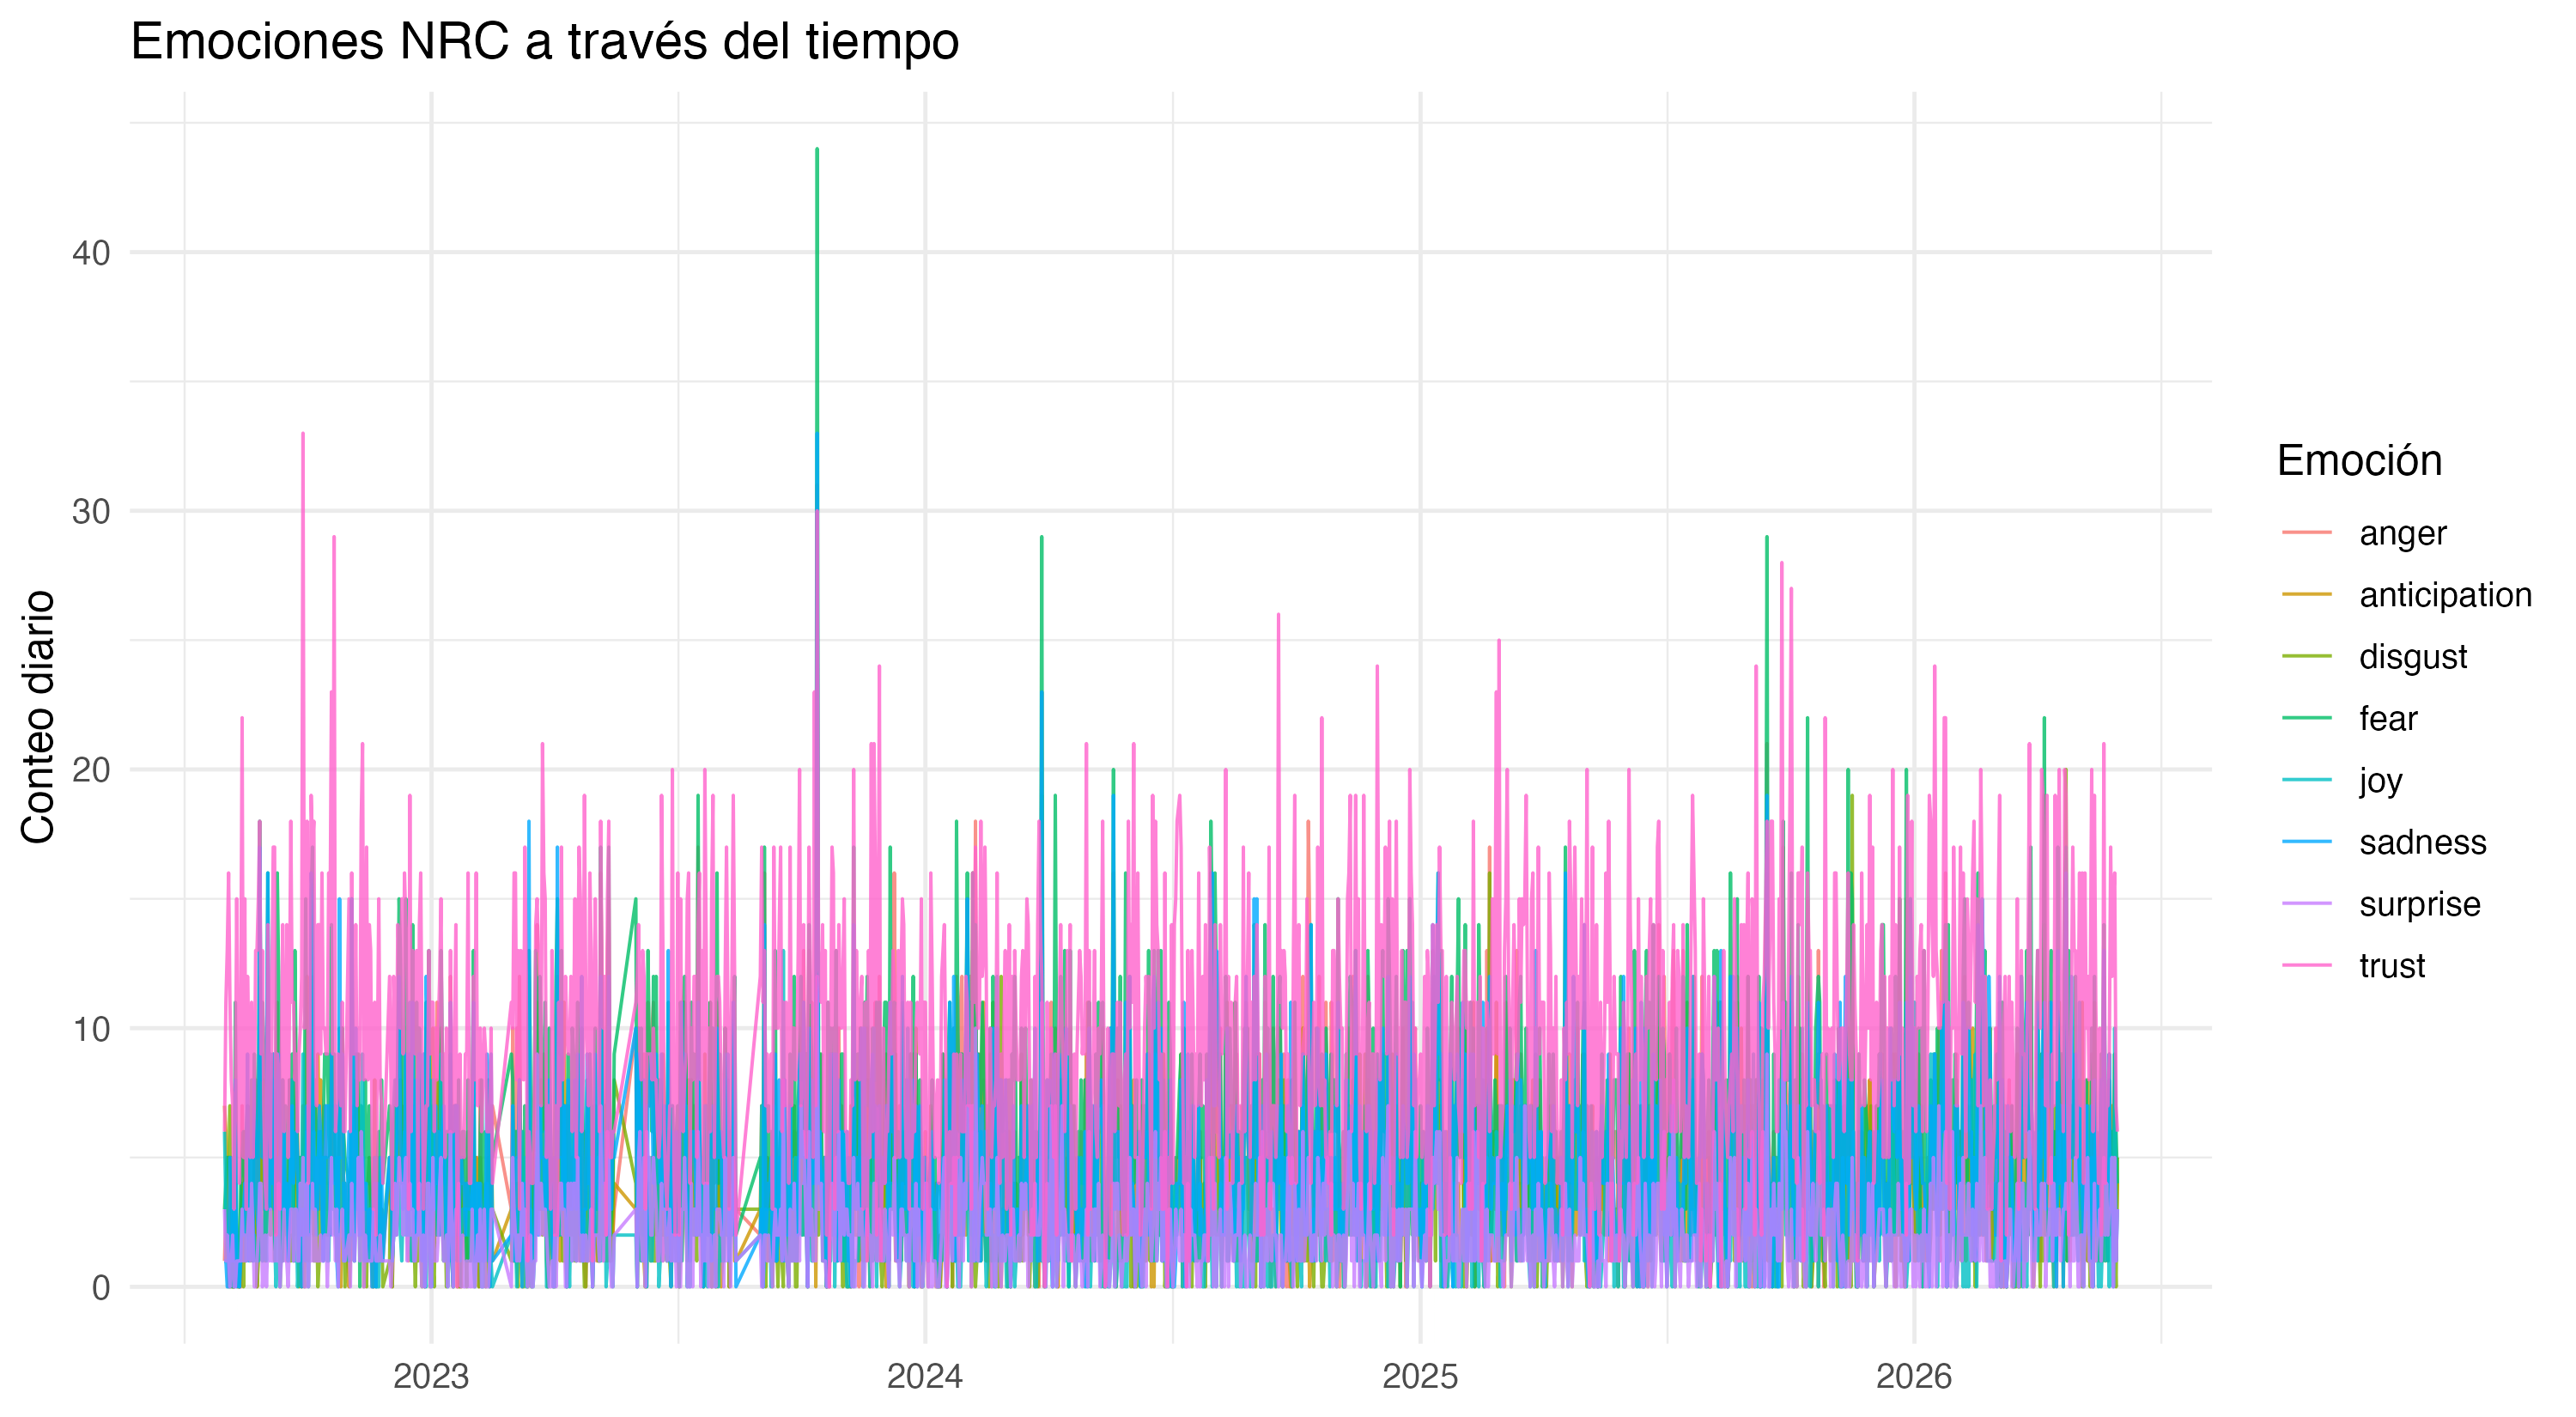
\includegraphics[width=0.9\linewidth,height=\textheight,keepaspectratio]{figures/sentimiento_emociones_diarias.png}

}

\caption{\label{fig-nrc}Emociones NRC a través del tiempo.}

\end{figure}%

\begin{figure}

\centering{

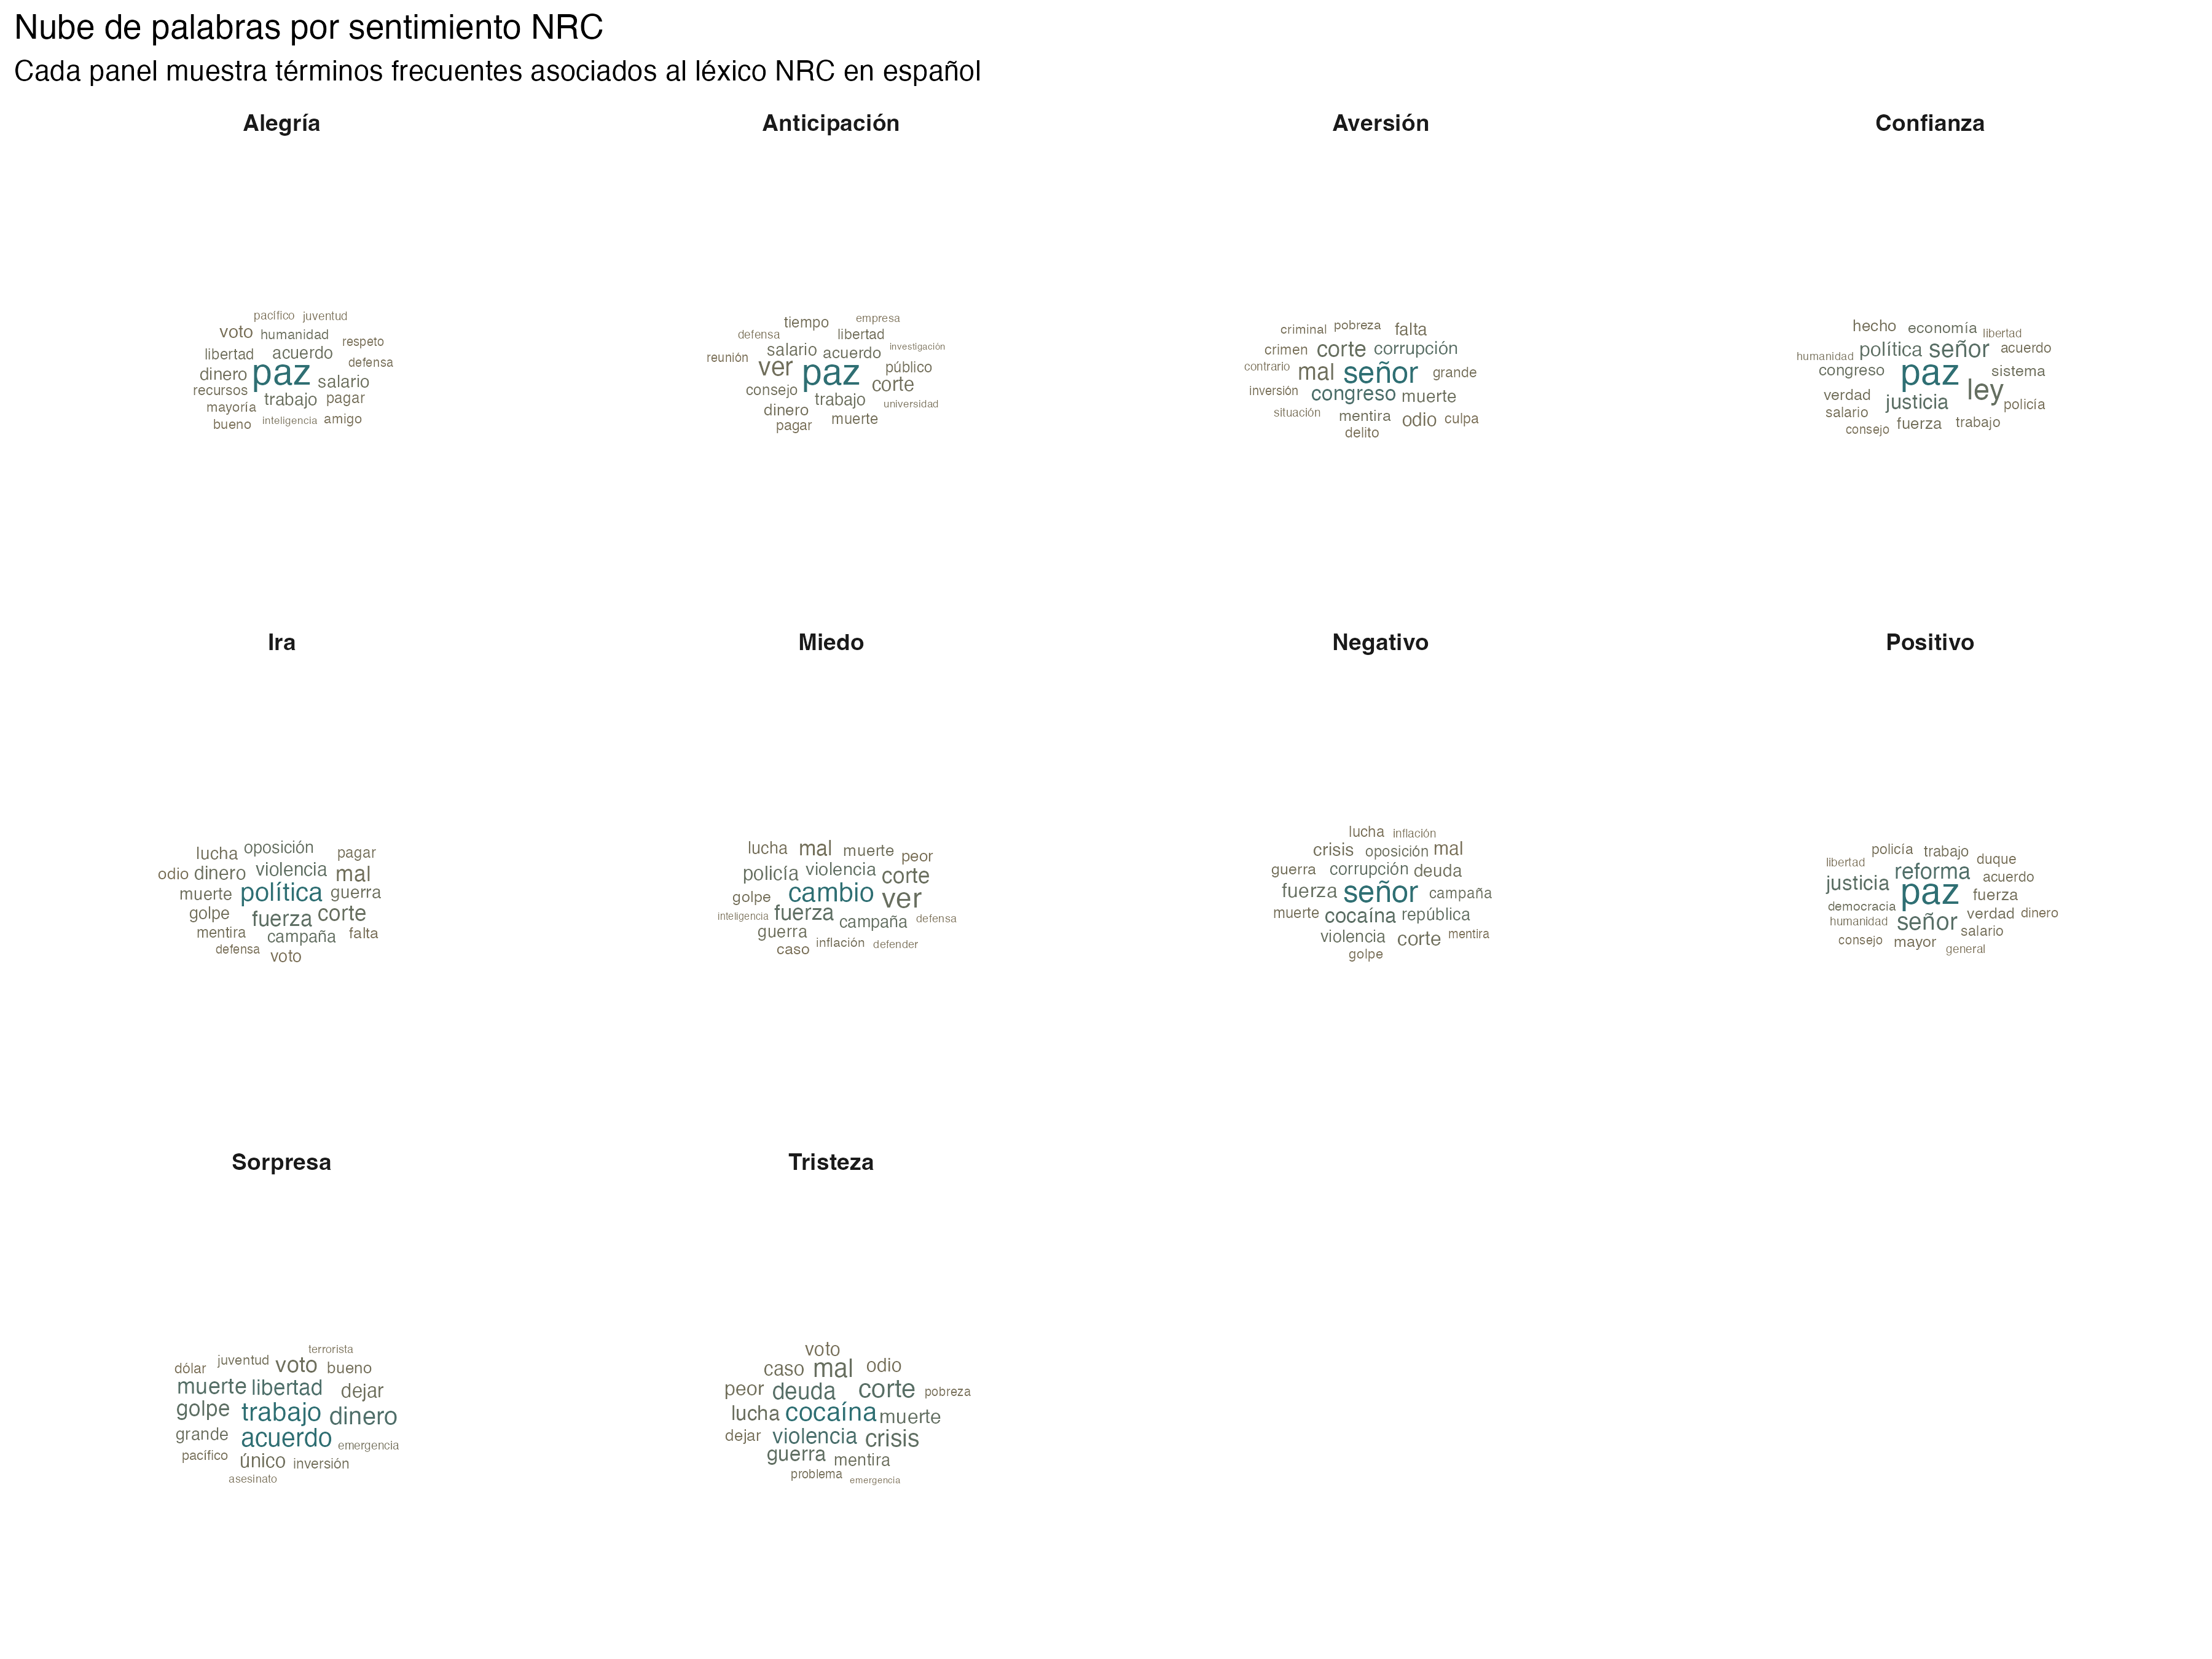
\includegraphics[width=0.9\linewidth,height=\textheight,keepaspectratio]{figures/wordcloud_sentimientos_nrc.png}

}

\caption{\label{fig-sentiment-cloud}Nube de palabras asociadas a
emociones y polaridad NRC.}

\end{figure}%

\begin{figure}

\centering{

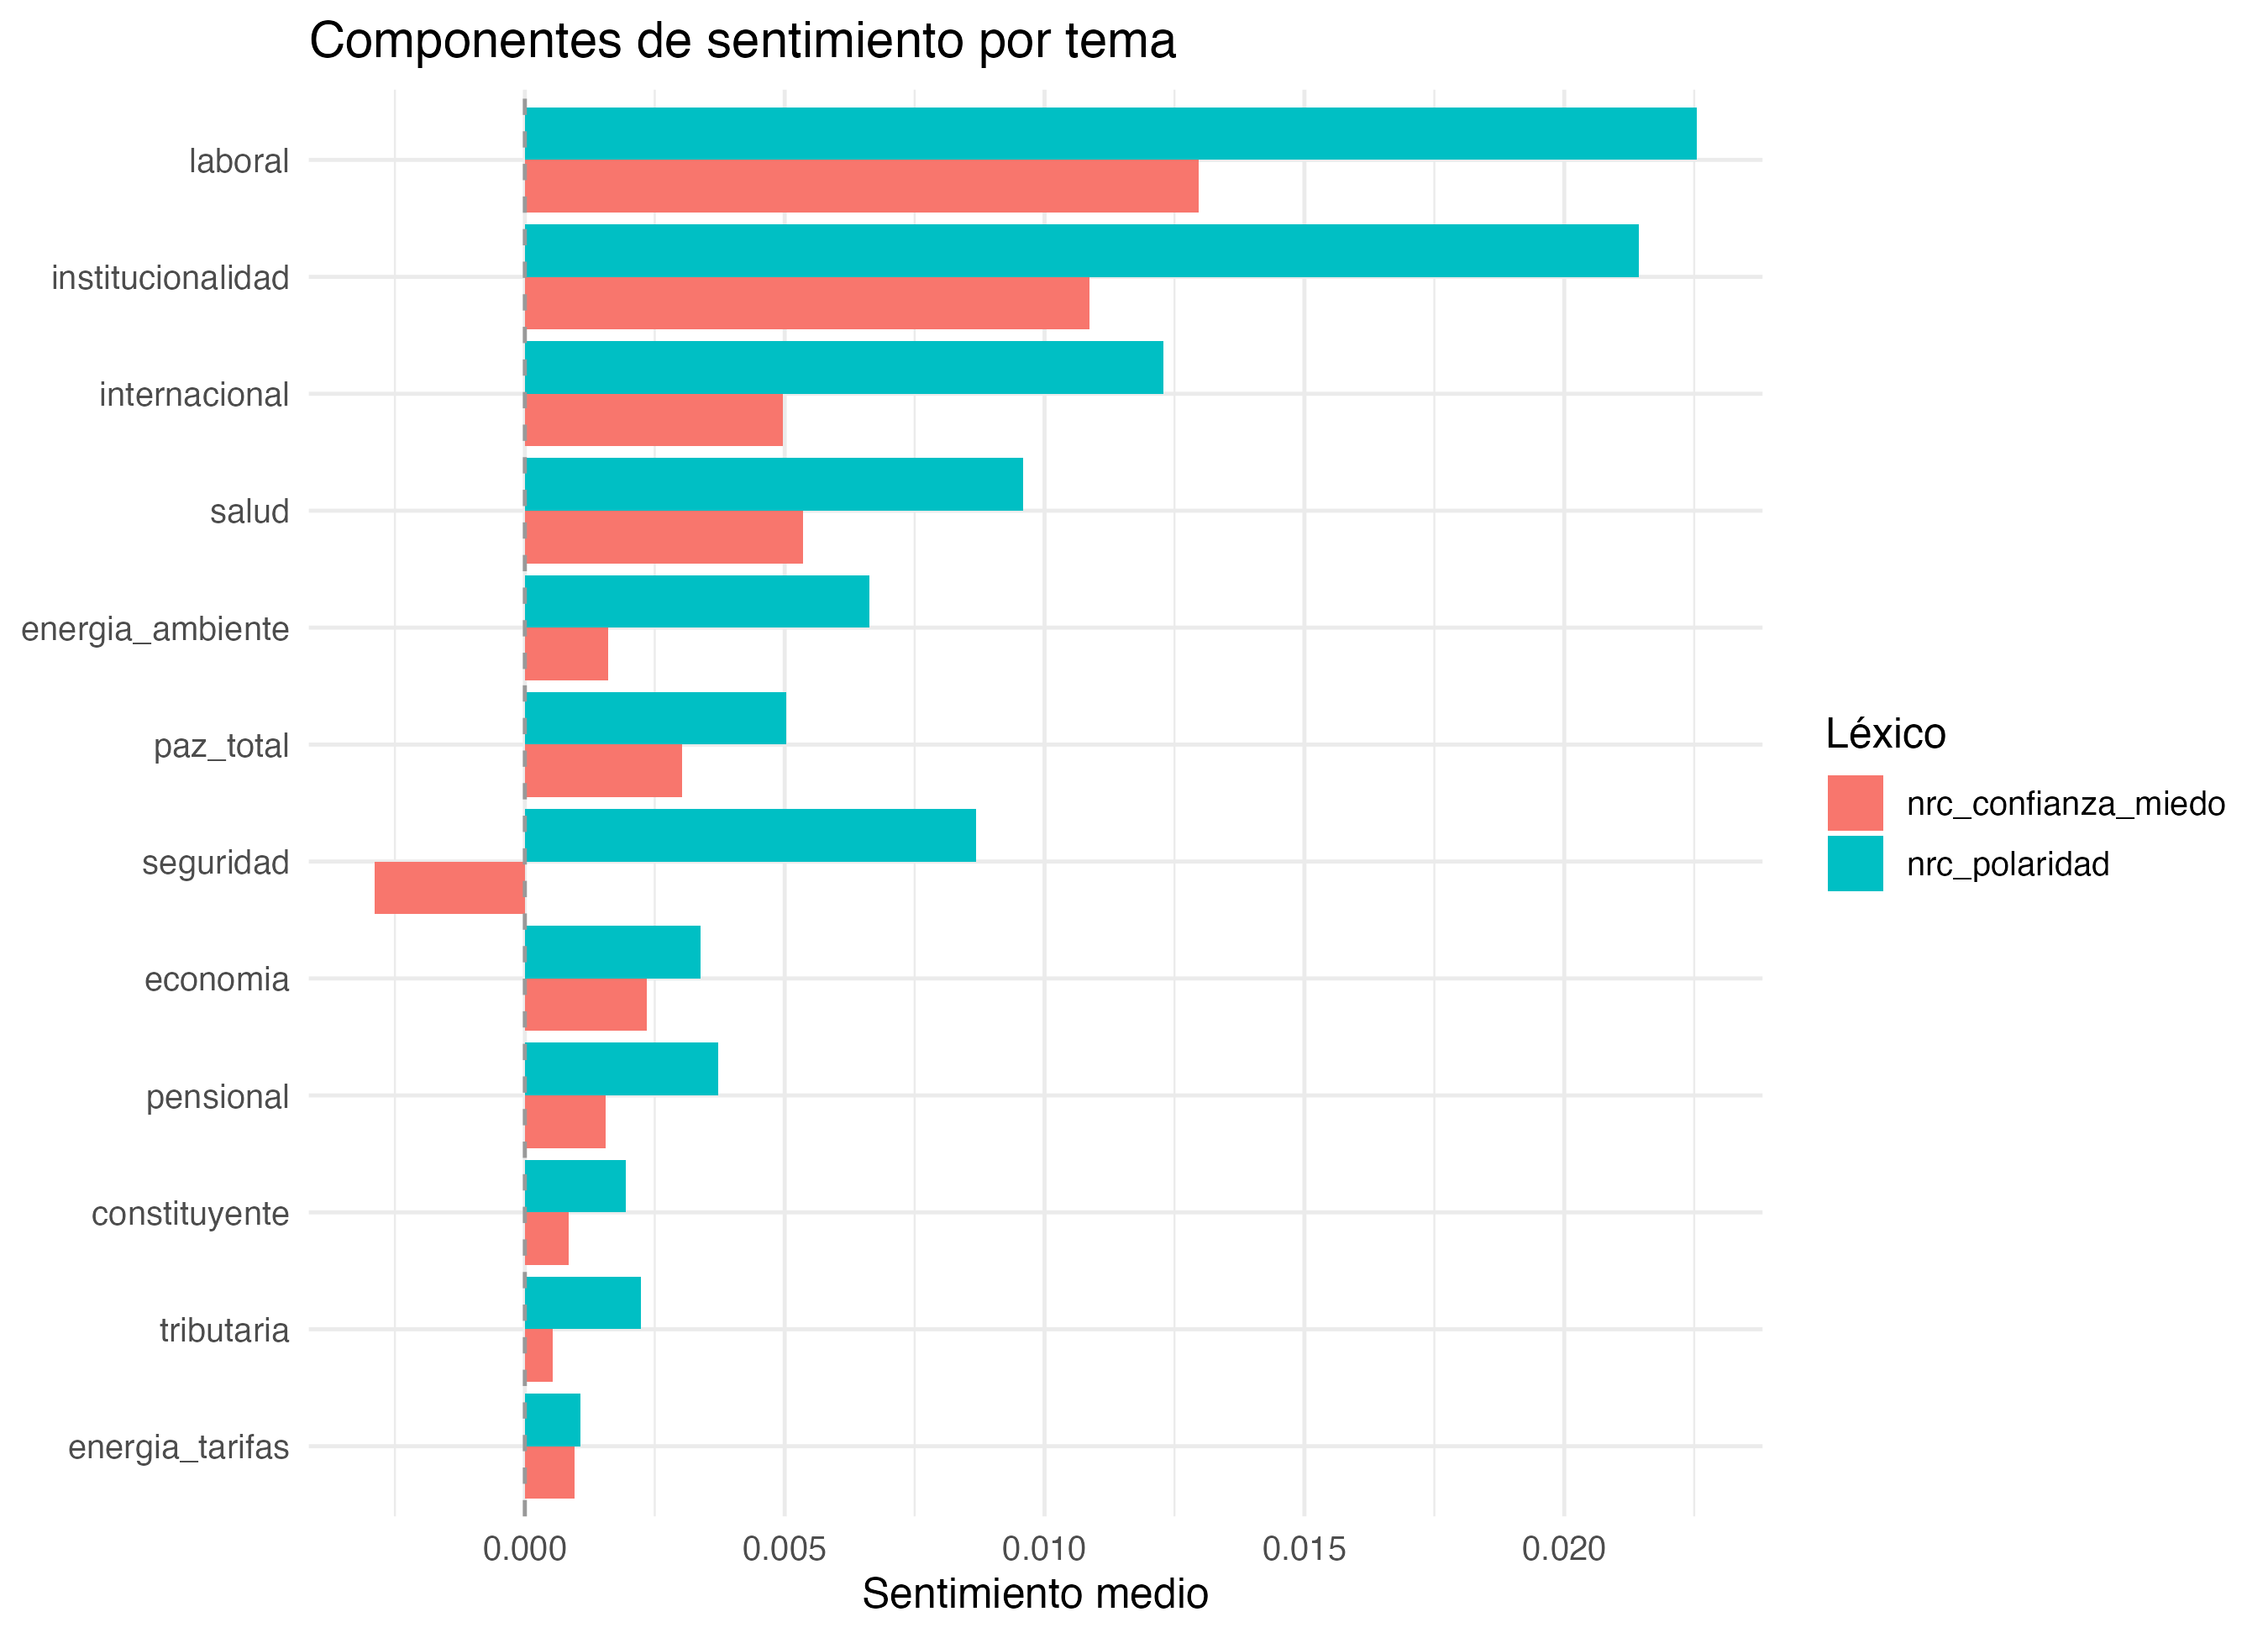
\includegraphics[width=0.9\linewidth,height=\textheight,keepaspectratio]{figures/sentometrics_componentes_lexicon.png}

}

\caption{\label{fig-sentometrics}Componentes sentometrics por lexicón y
tema.}

\end{figure}%

El enriquecimiento lingüístico con spaCy aporta una lectura adicional de
paz total. La versión original se concentraba en reformas y hashtags
asociados a Petro; la actualización separa paz total porque conecta
seguridad, negociación, actores armados, Estado y expectativas
institucionales. Las entidades y lemas ayudan a identificar actores y
términos de política pública que aparecen de forma recurrente en esa
conversación.

\begin{figure}

\centering{

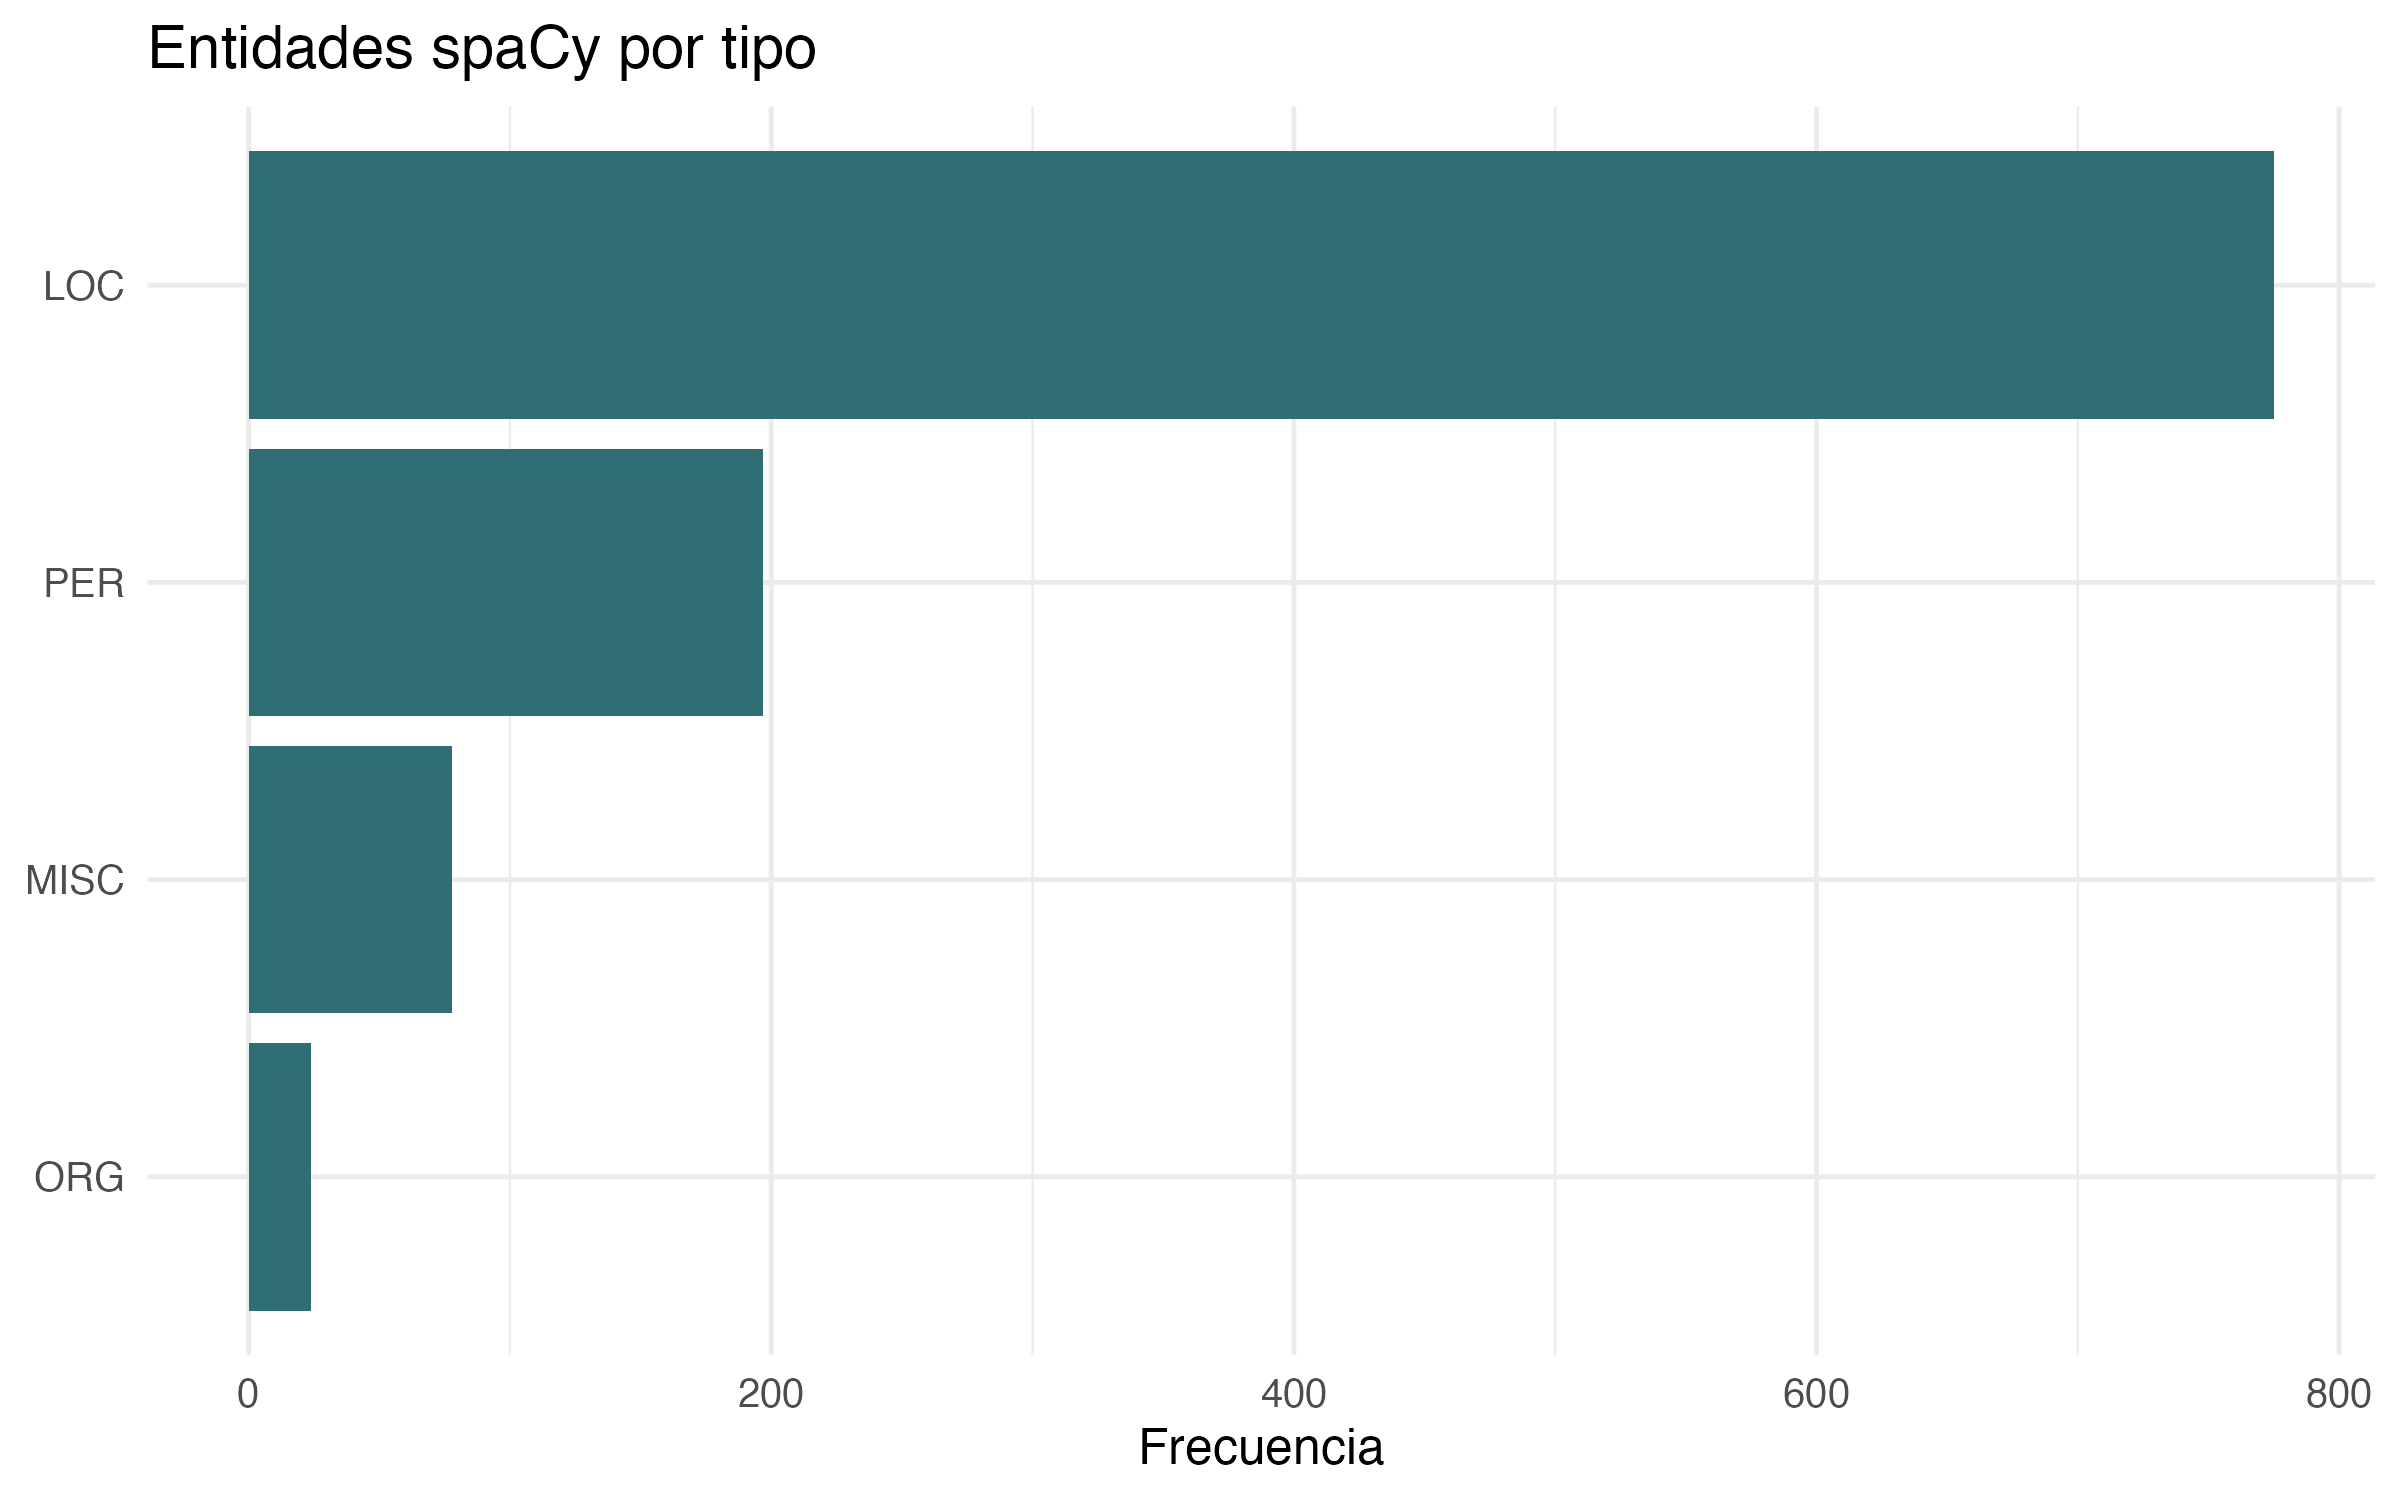
\includegraphics[width=0.8\linewidth,height=\textheight,keepaspectratio]{figures/spacyr_entidades_tipo.png}

}

\caption{\label{fig-spacy}Tipos de entidades extraídas con spaCy
mediante spacyr.}

\end{figure}%

El bloque de mercado usa TRM para el canal cambiario, COLCAP para el
canal accionario y TES para el canal de renta fija soberana. Esta
ampliación es importante porque un mensaje político puede afectar de
manera diferente expectativas sobre moneda, acciones y tasas soberanas.
La curva TES permite observar variaciones de corto y largo plazo, y la
pendiente 10Y-1Y resume cambios en la lectura intertemporal del riesgo.

\begin{figure}

\centering{

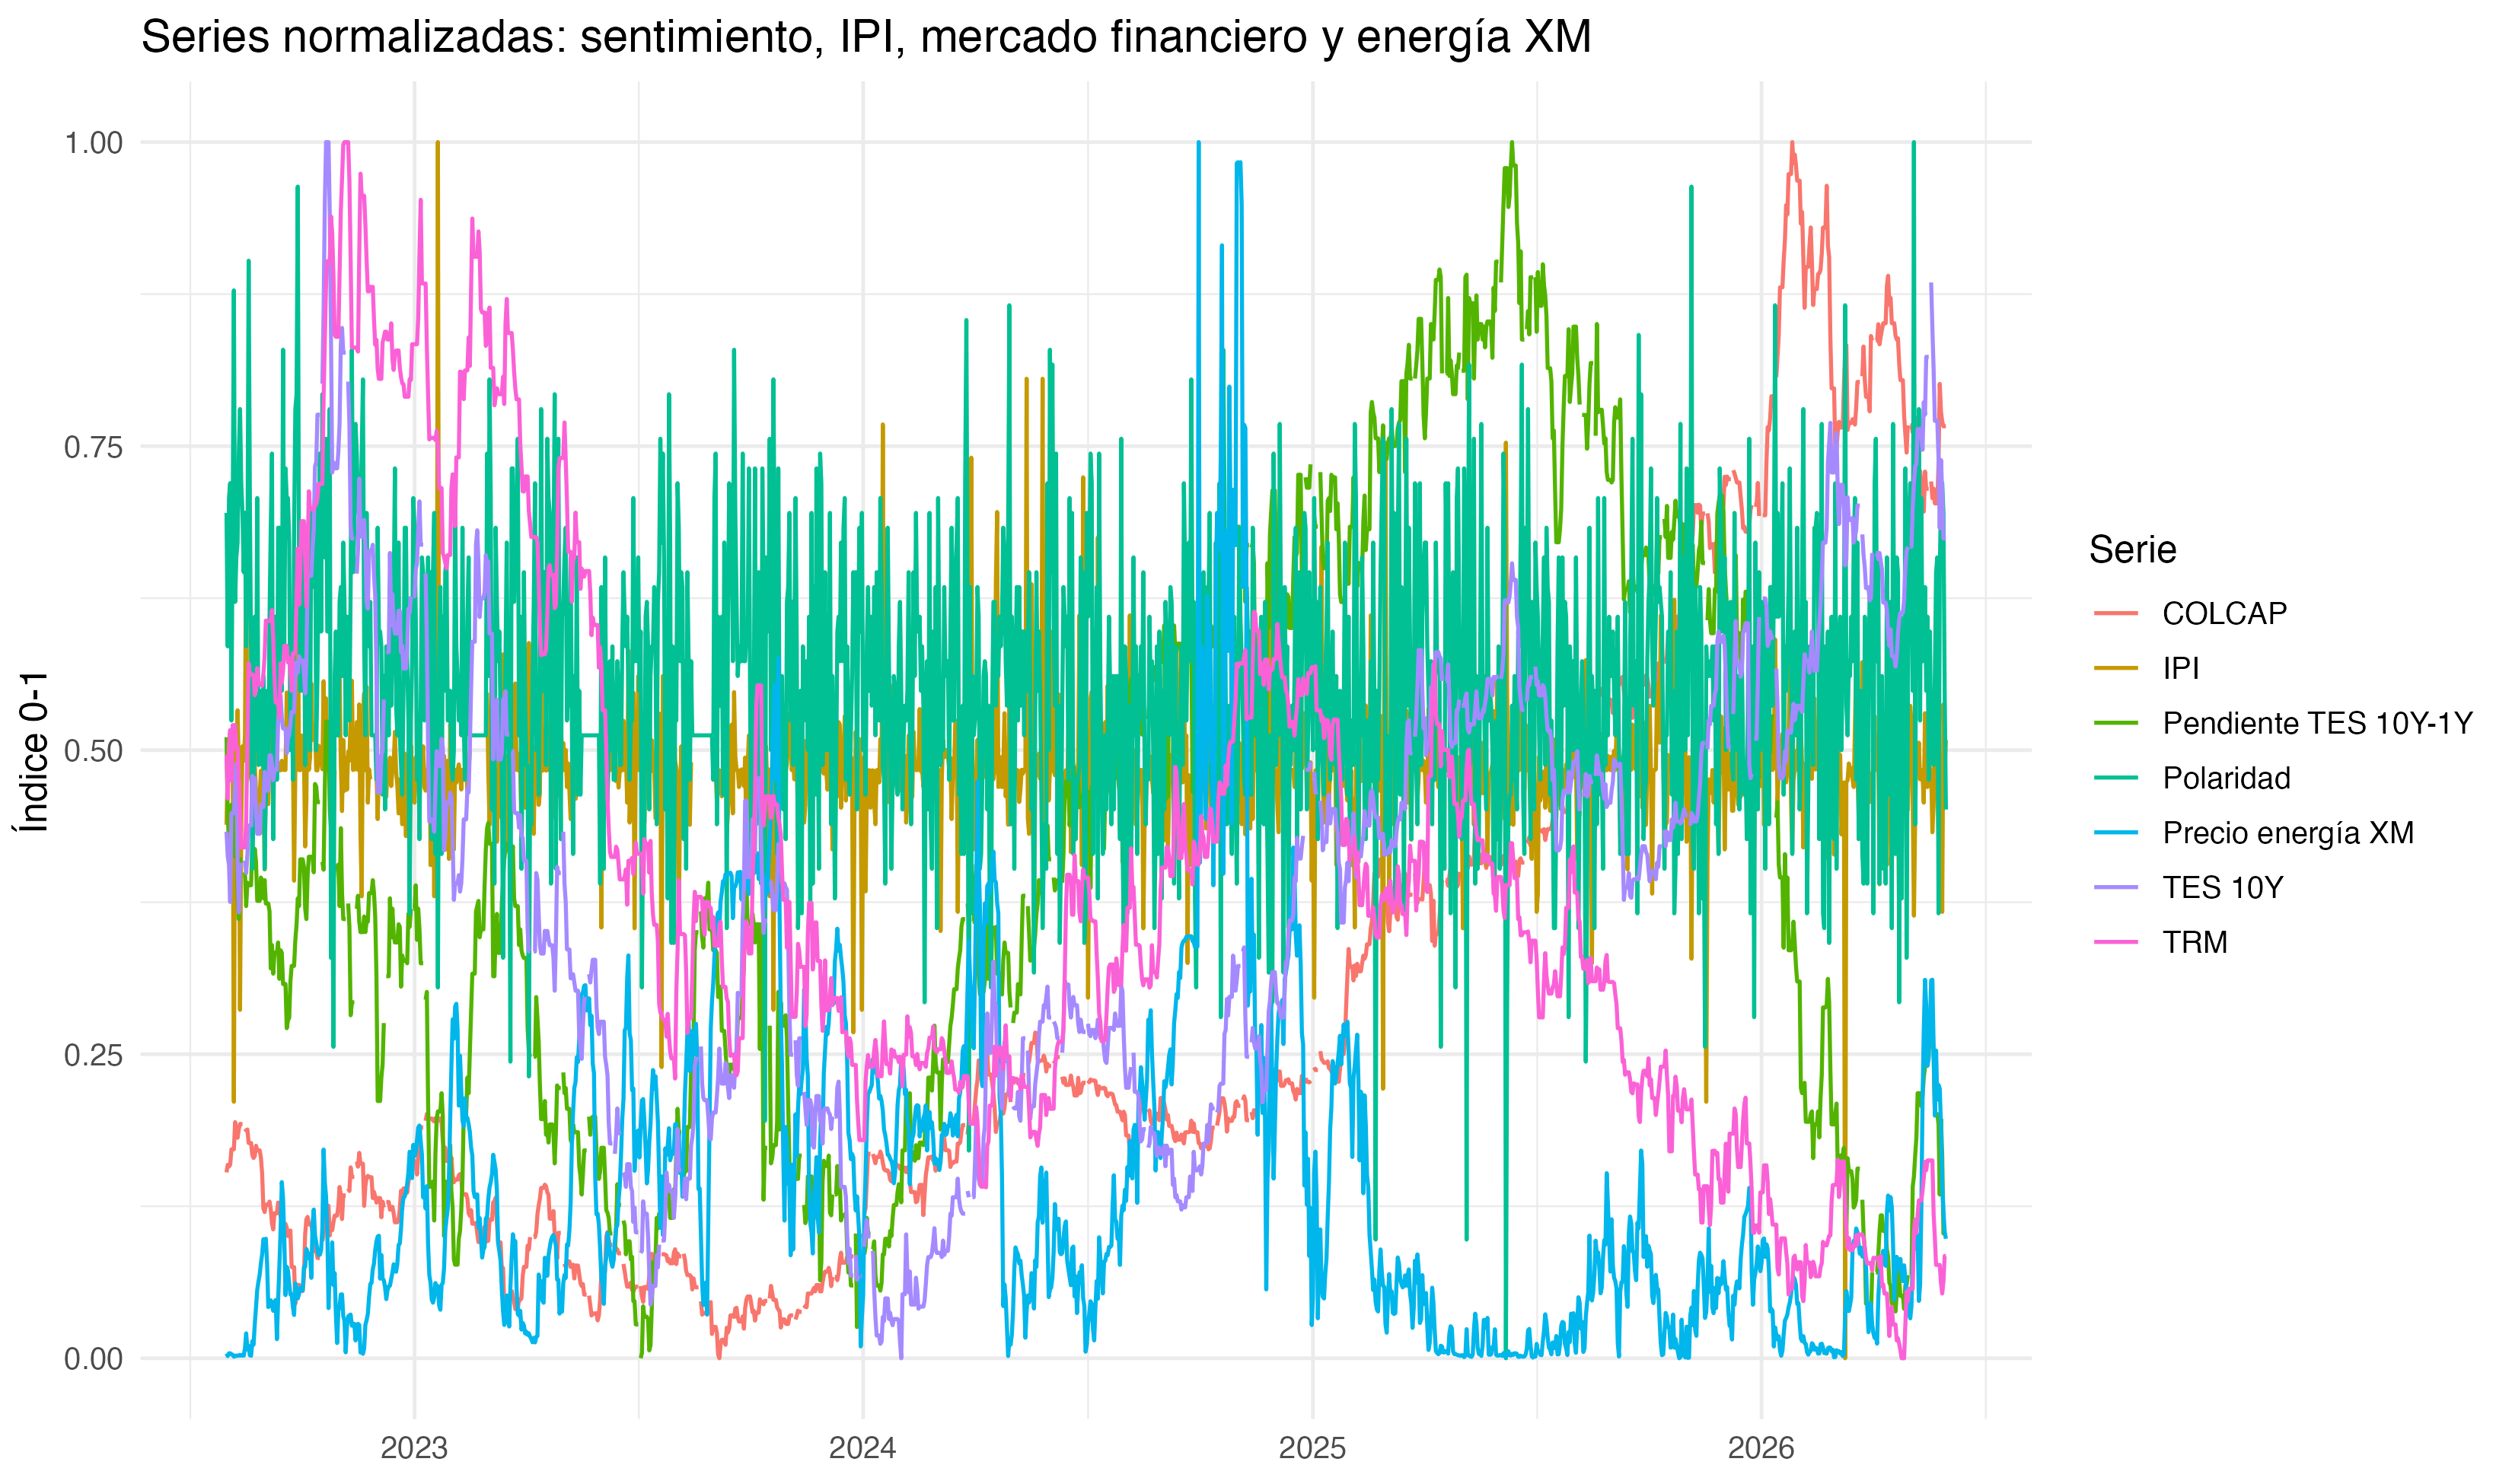
\includegraphics[width=0.9\linewidth,height=\textheight,keepaspectratio]{figures/serie_sentimientos_trm_colcap.png}

}

\caption{\label{fig-series}Series normalizadas de tweets, sentimiento,
TRM, COLCAP y TES.}

\end{figure}%

\begin{figure}

\centering{

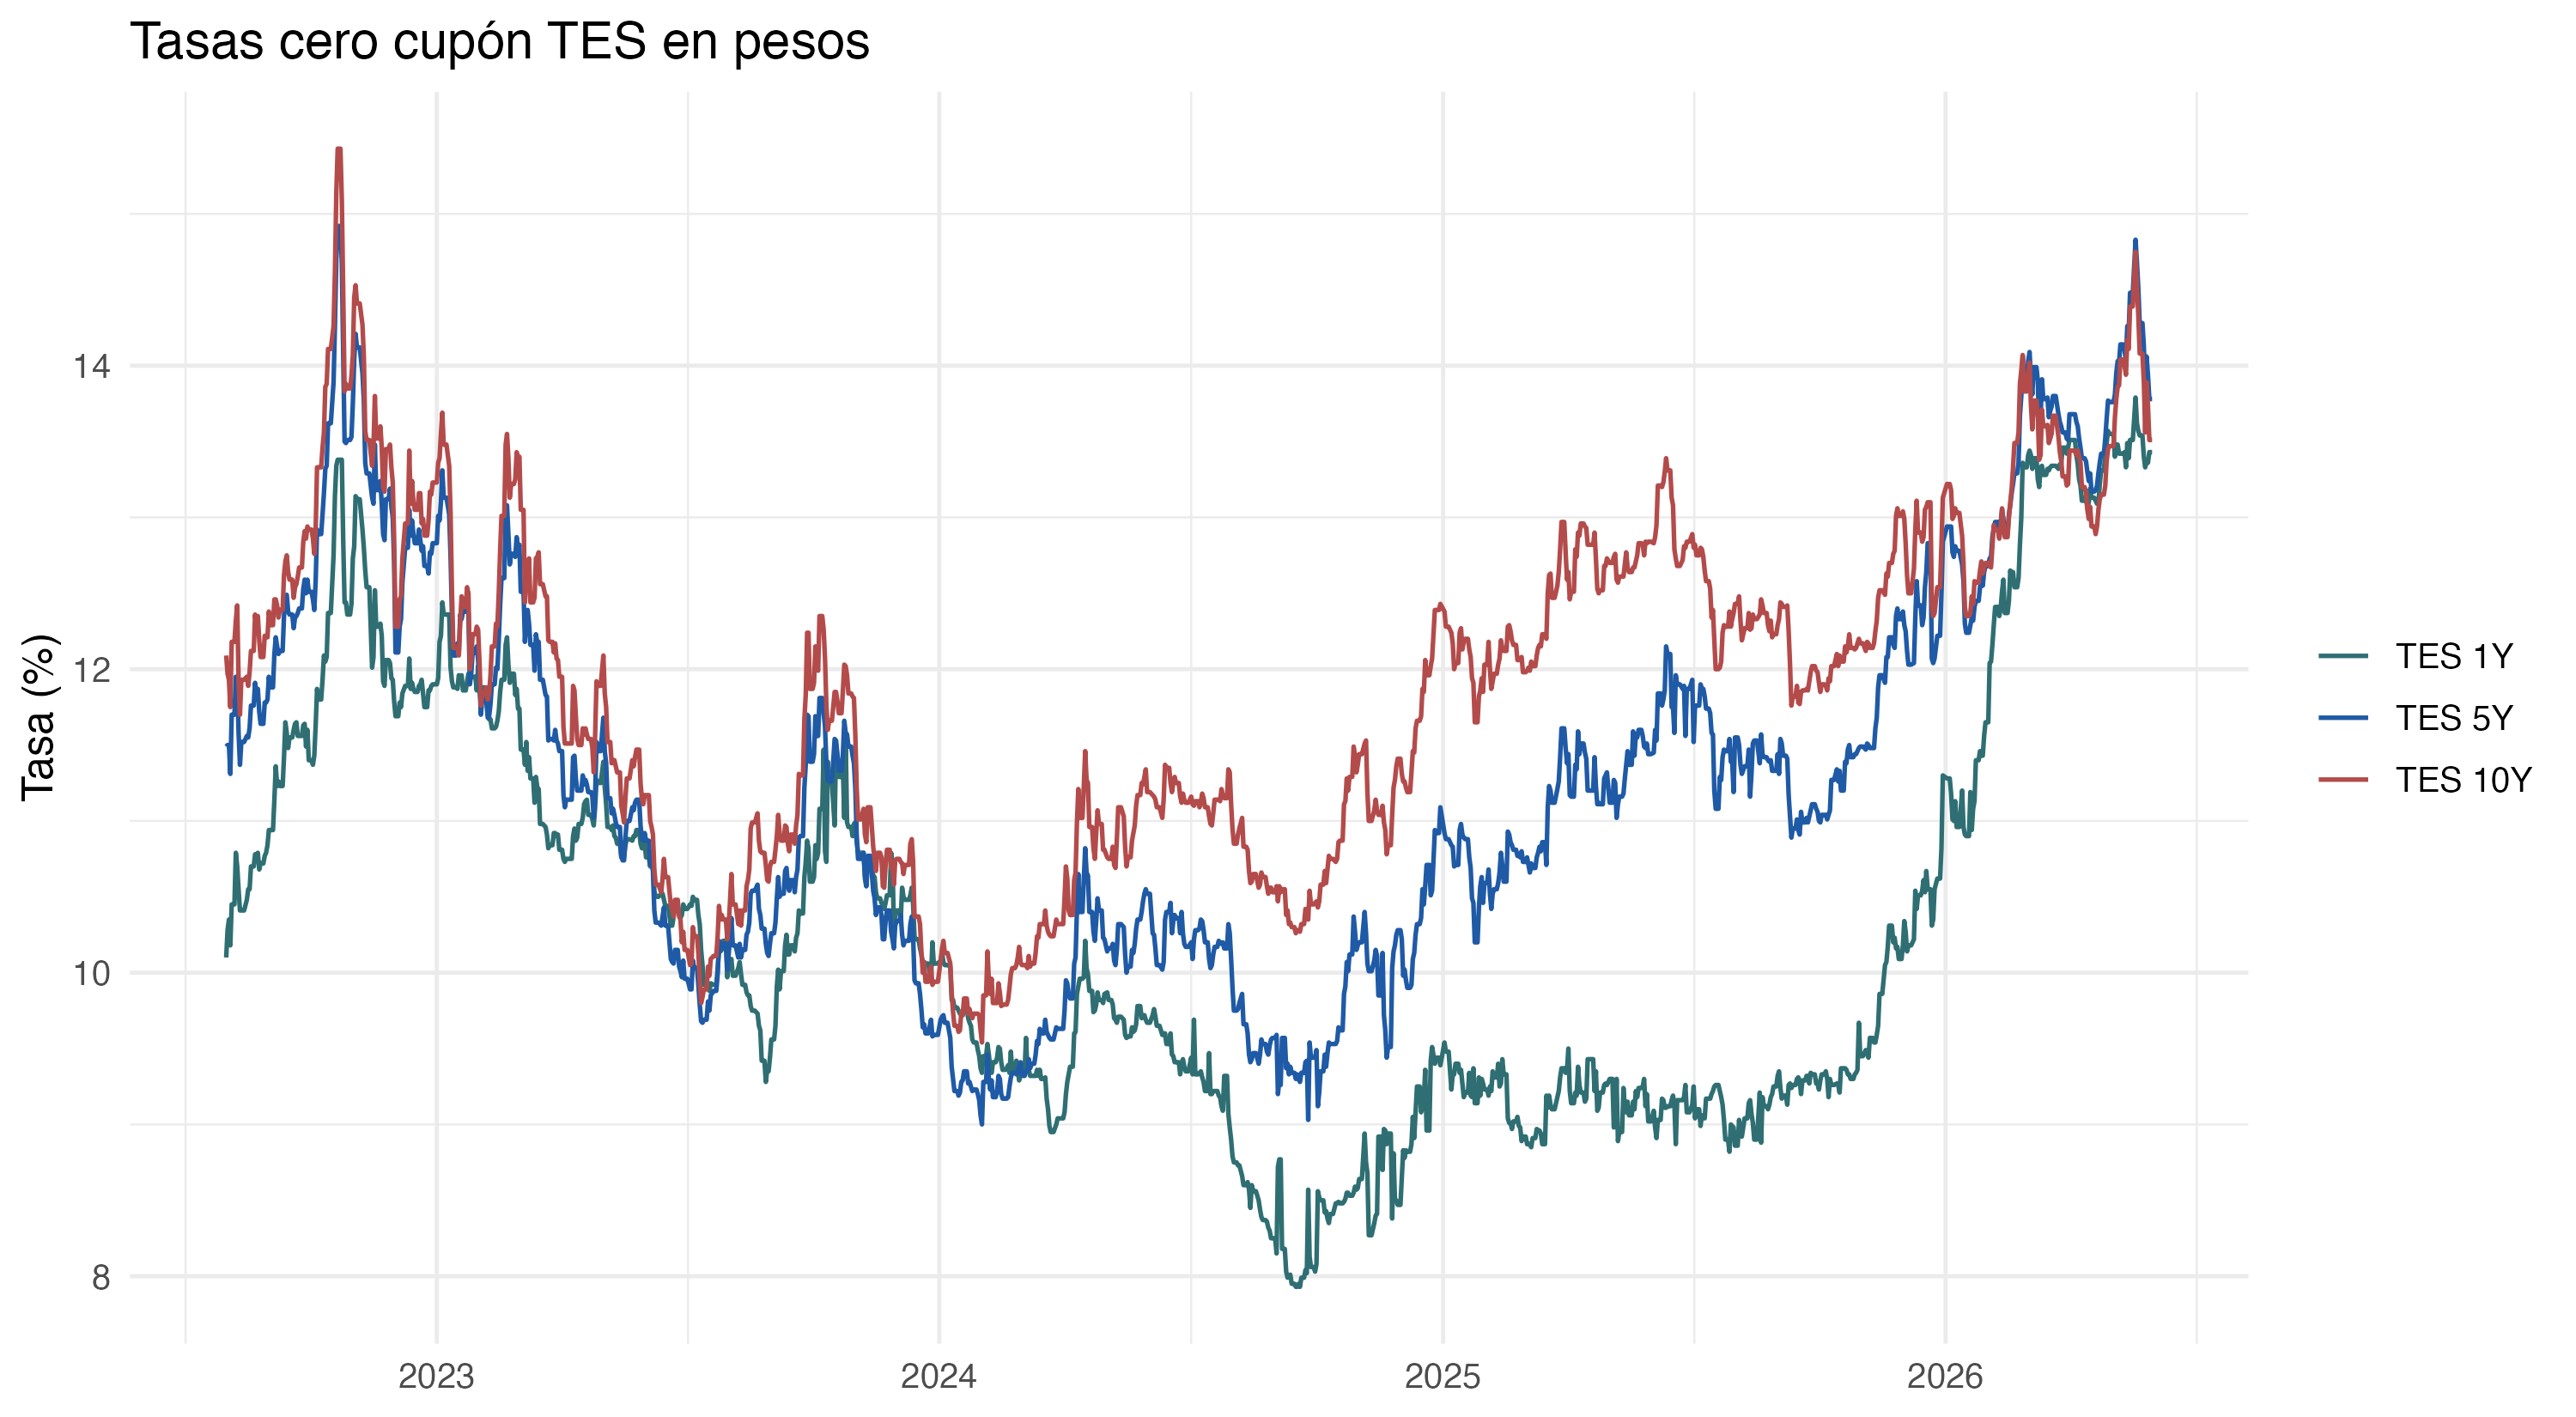
\includegraphics[width=0.9\linewidth,height=\textheight,keepaspectratio]{figures/tes_curva_cero_cupon.png}

}

\caption{\label{fig-tes-curve}Tasas cero cupón TES en pesos.}

\end{figure}%

\begin{figure}

\centering{

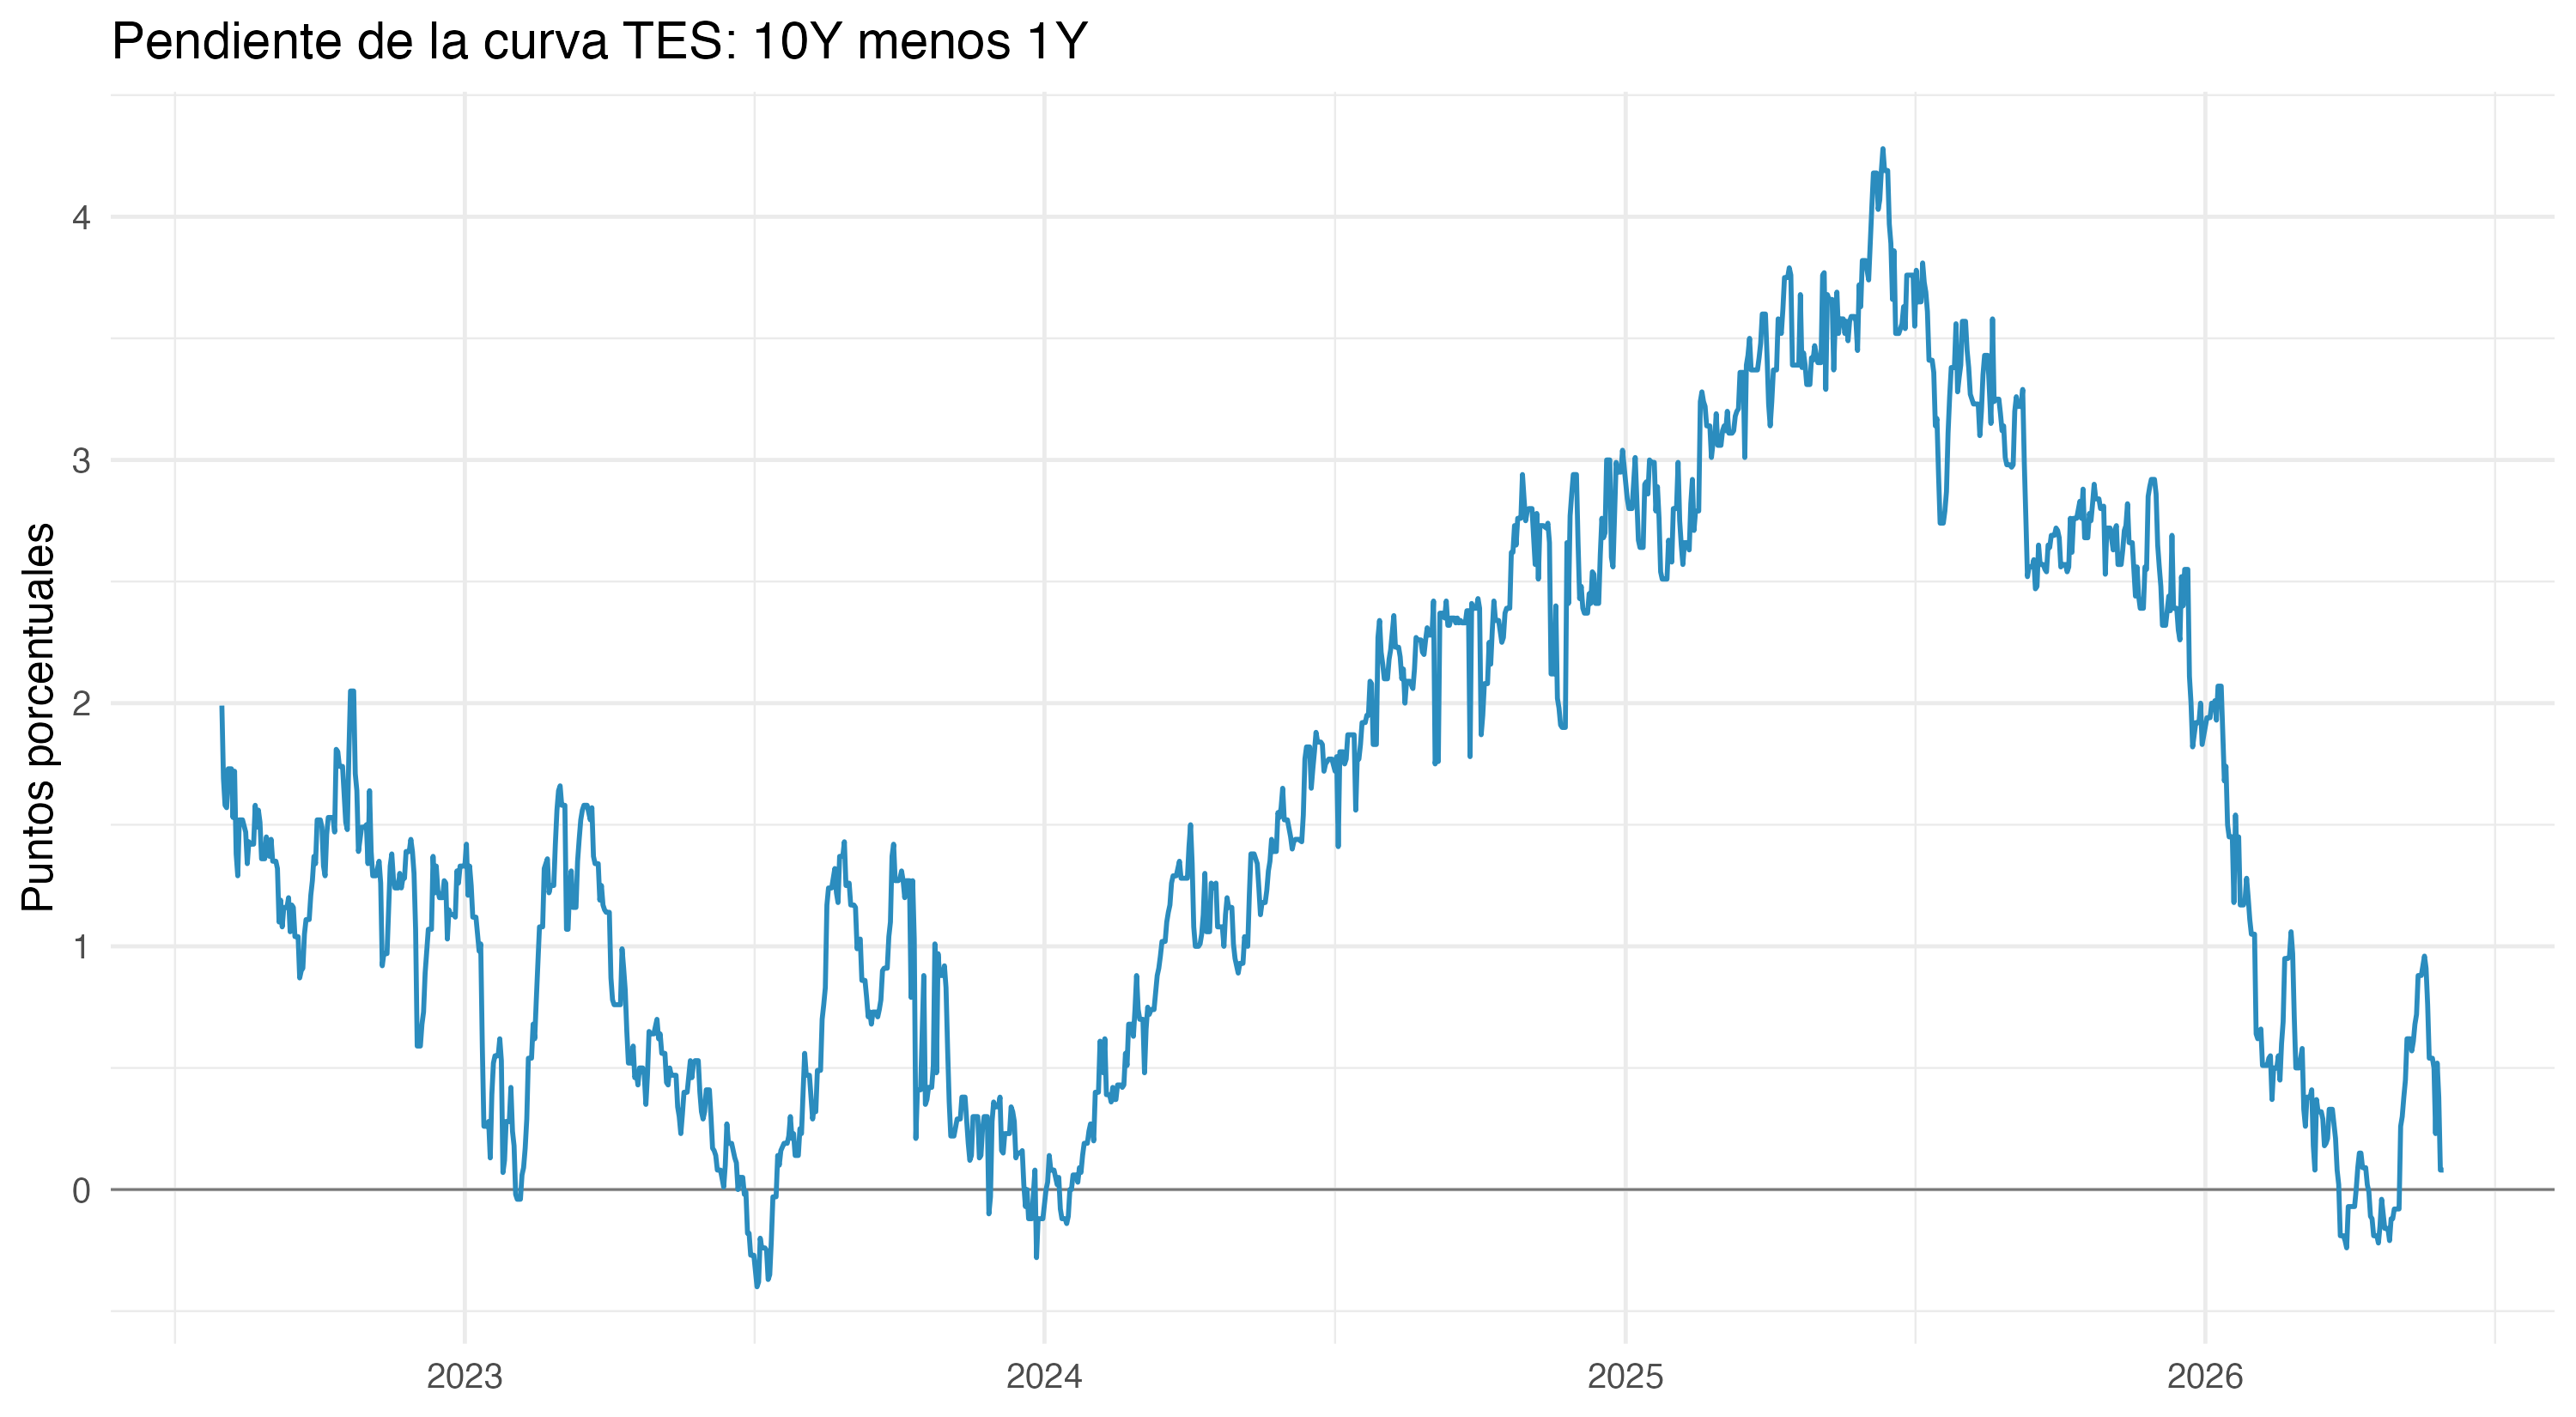
\includegraphics[width=0.9\linewidth,height=\textheight,keepaspectratio]{figures/tes_pendiente_10y_1y.png}

}

\caption{\label{fig-tes-slope}Pendiente de la curva soberana TES: 10Y
menos 1Y.}

\end{figure}%

Las pruebas de Granger se interpretan como diagnósticos de precedencia
temporal, no como causalidad estructural. Algunos indicadores de
sentimiento, volumen o presión informacional pueden mejorar la
predicción de respuestas específicas en ciertos rezagos, y ahora esa
evaluación se reporta por corpus. Esto no demuestra que los tweets
causen movimientos financieros: compara si la conversación pública y el
discurso presidencial directo aportan señales predictivas exploratorias
distintas. El estudio de eventos complementa esta lectura al describir
qué ocurre después de días extremos de negatividad, volumen o presión
informacional. TRM y COLCAP se leen como retornos, mientras TES 10Y y la
pendiente se leen como cambios en tasas.

\begin{figure}

\centering{

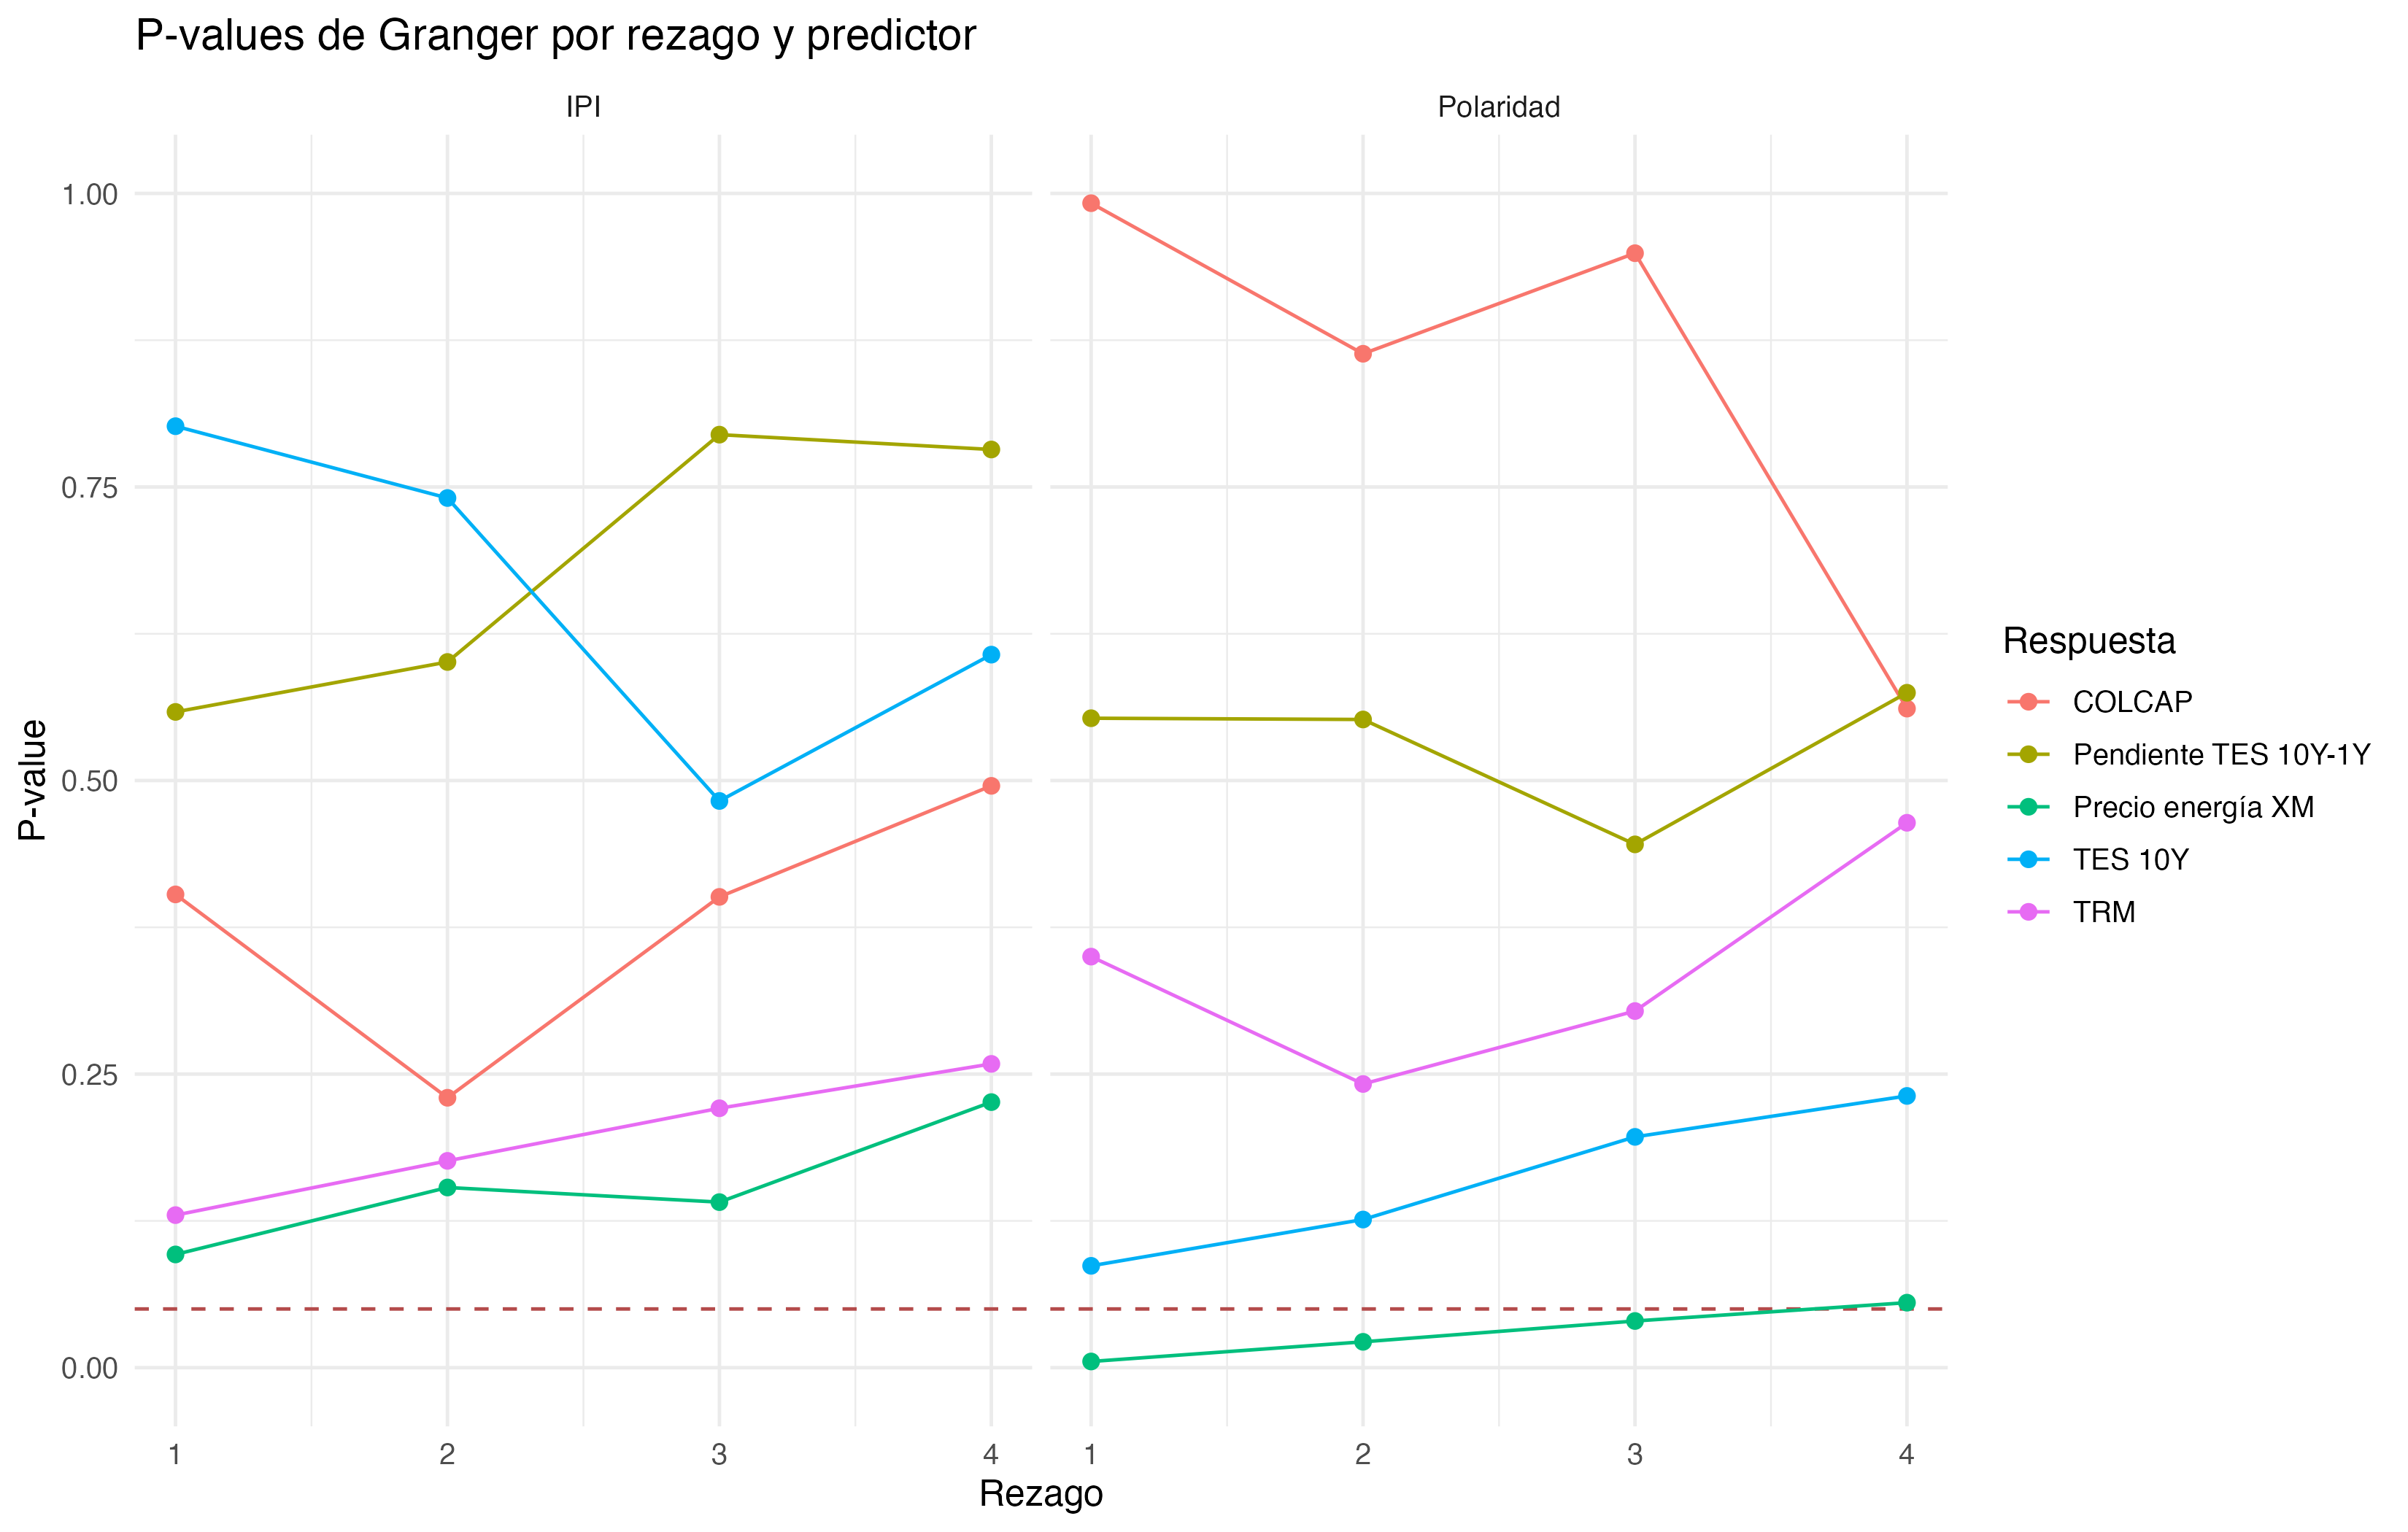
\includegraphics[width=0.9\linewidth,height=\textheight,keepaspectratio]{figures/granger_trm_colcap.png}

}

\caption{\label{fig-granger}Valores p de Granger por rezago y respuesta
de mercado.}

\end{figure}%

\begin{figure}

\centering{

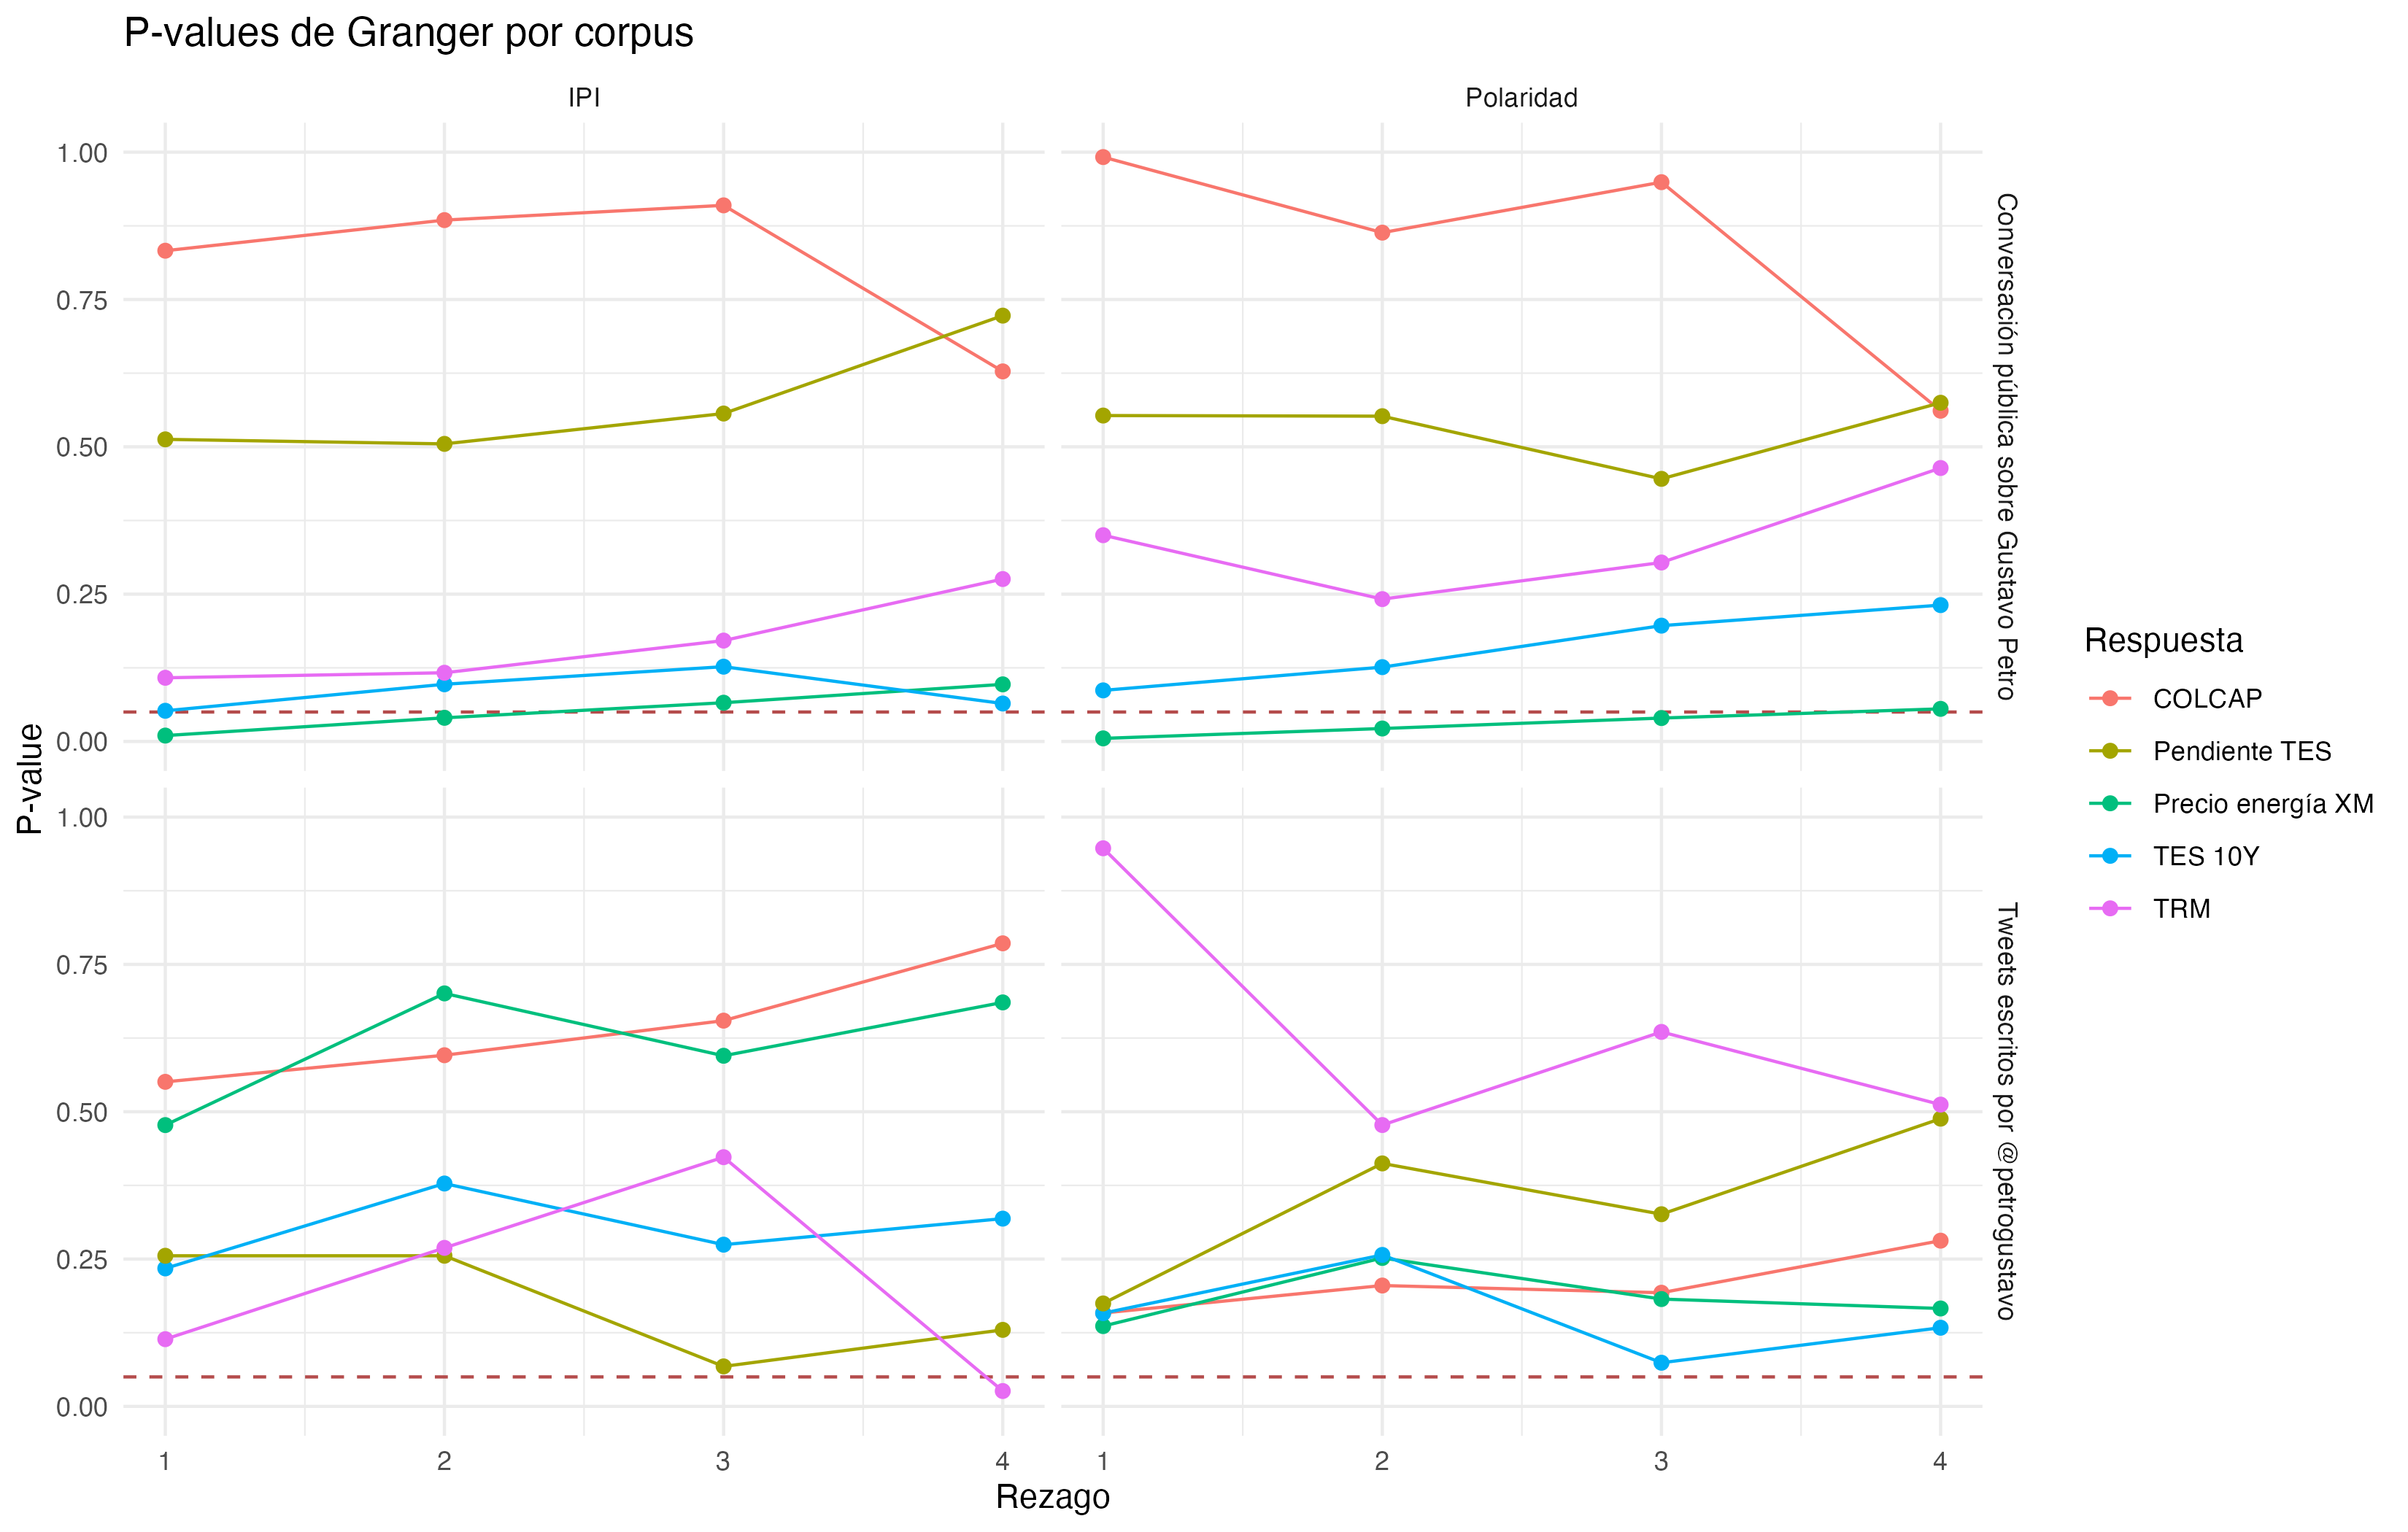
\includegraphics[width=0.9\linewidth,height=\textheight,keepaspectratio]{figures/granger_por_corpus.png}

}

\caption{\label{fig-granger-corpus}Valores p de Granger por corpus,
predictor y respuesta de mercado.}

\end{figure}%

\begin{figure}

\centering{

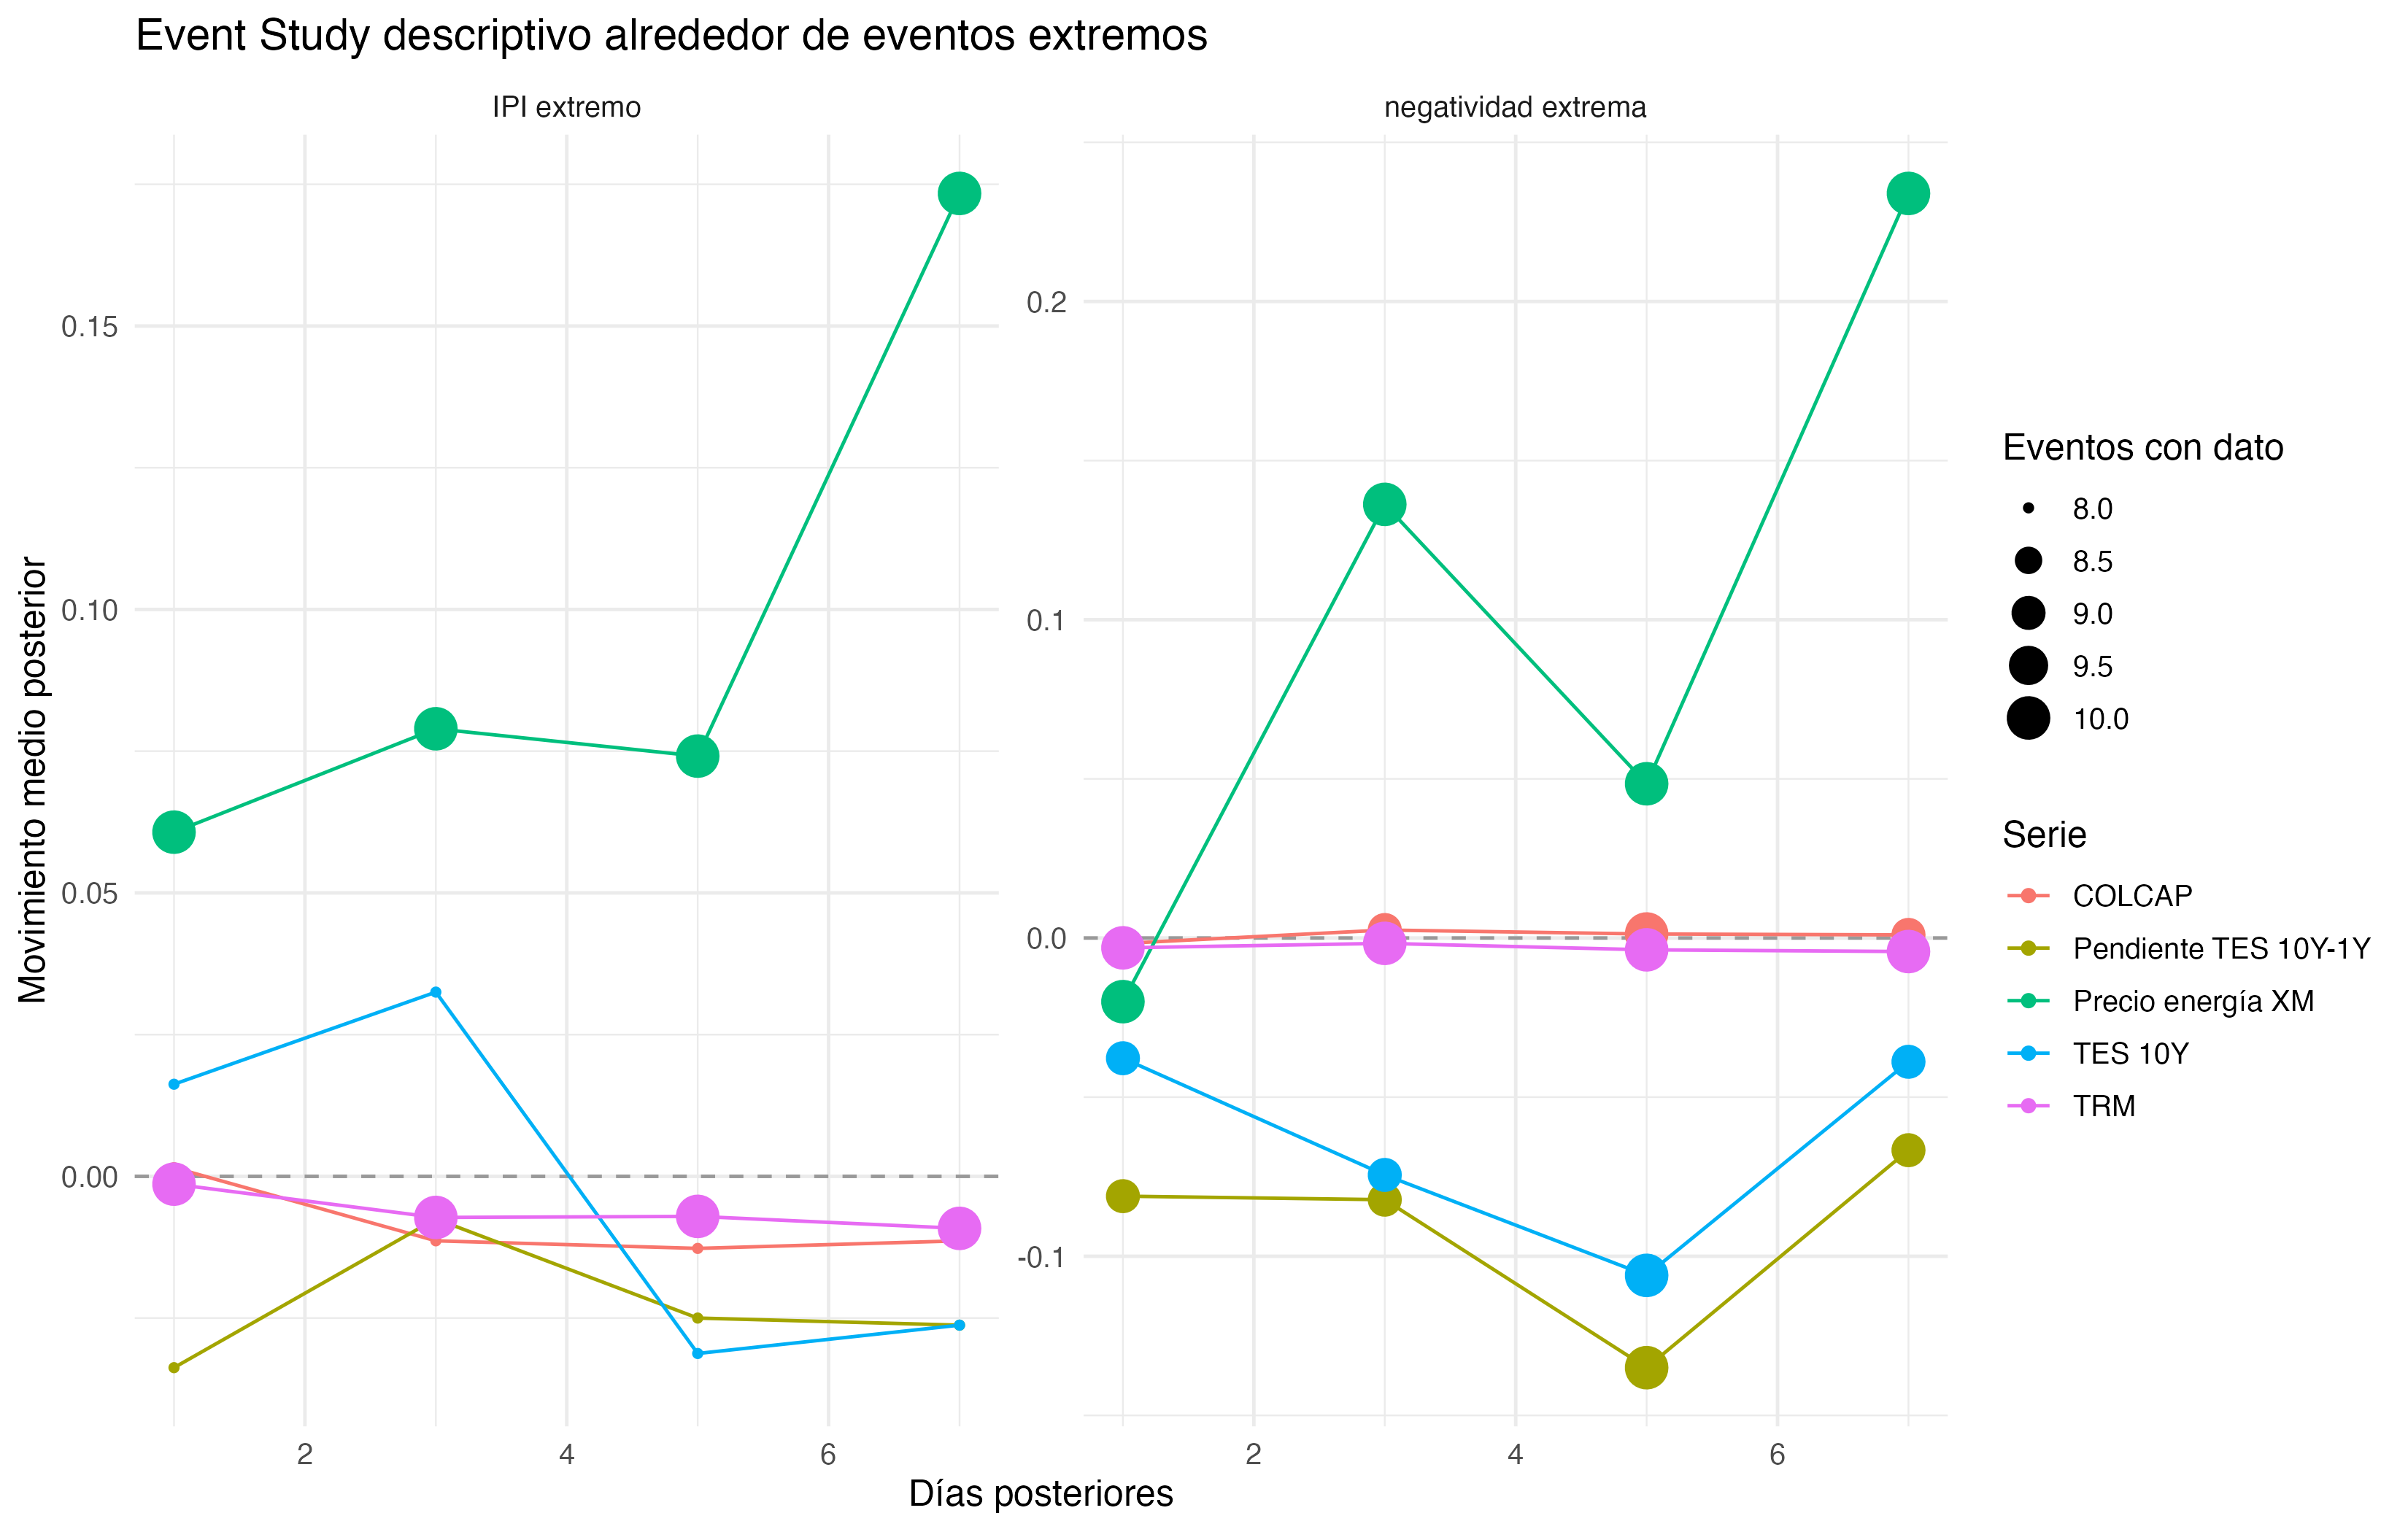
\includegraphics[width=0.9\linewidth,height=\textheight,keepaspectratio]{figures/event_study_ipi_trm_colcap.png}

}

\caption{\label{fig-event-study}Ventanas de estudio de eventos alrededor
de días extremos de sentimiento, volumen e IPI.}

\end{figure}%

\begin{figure}

\centering{

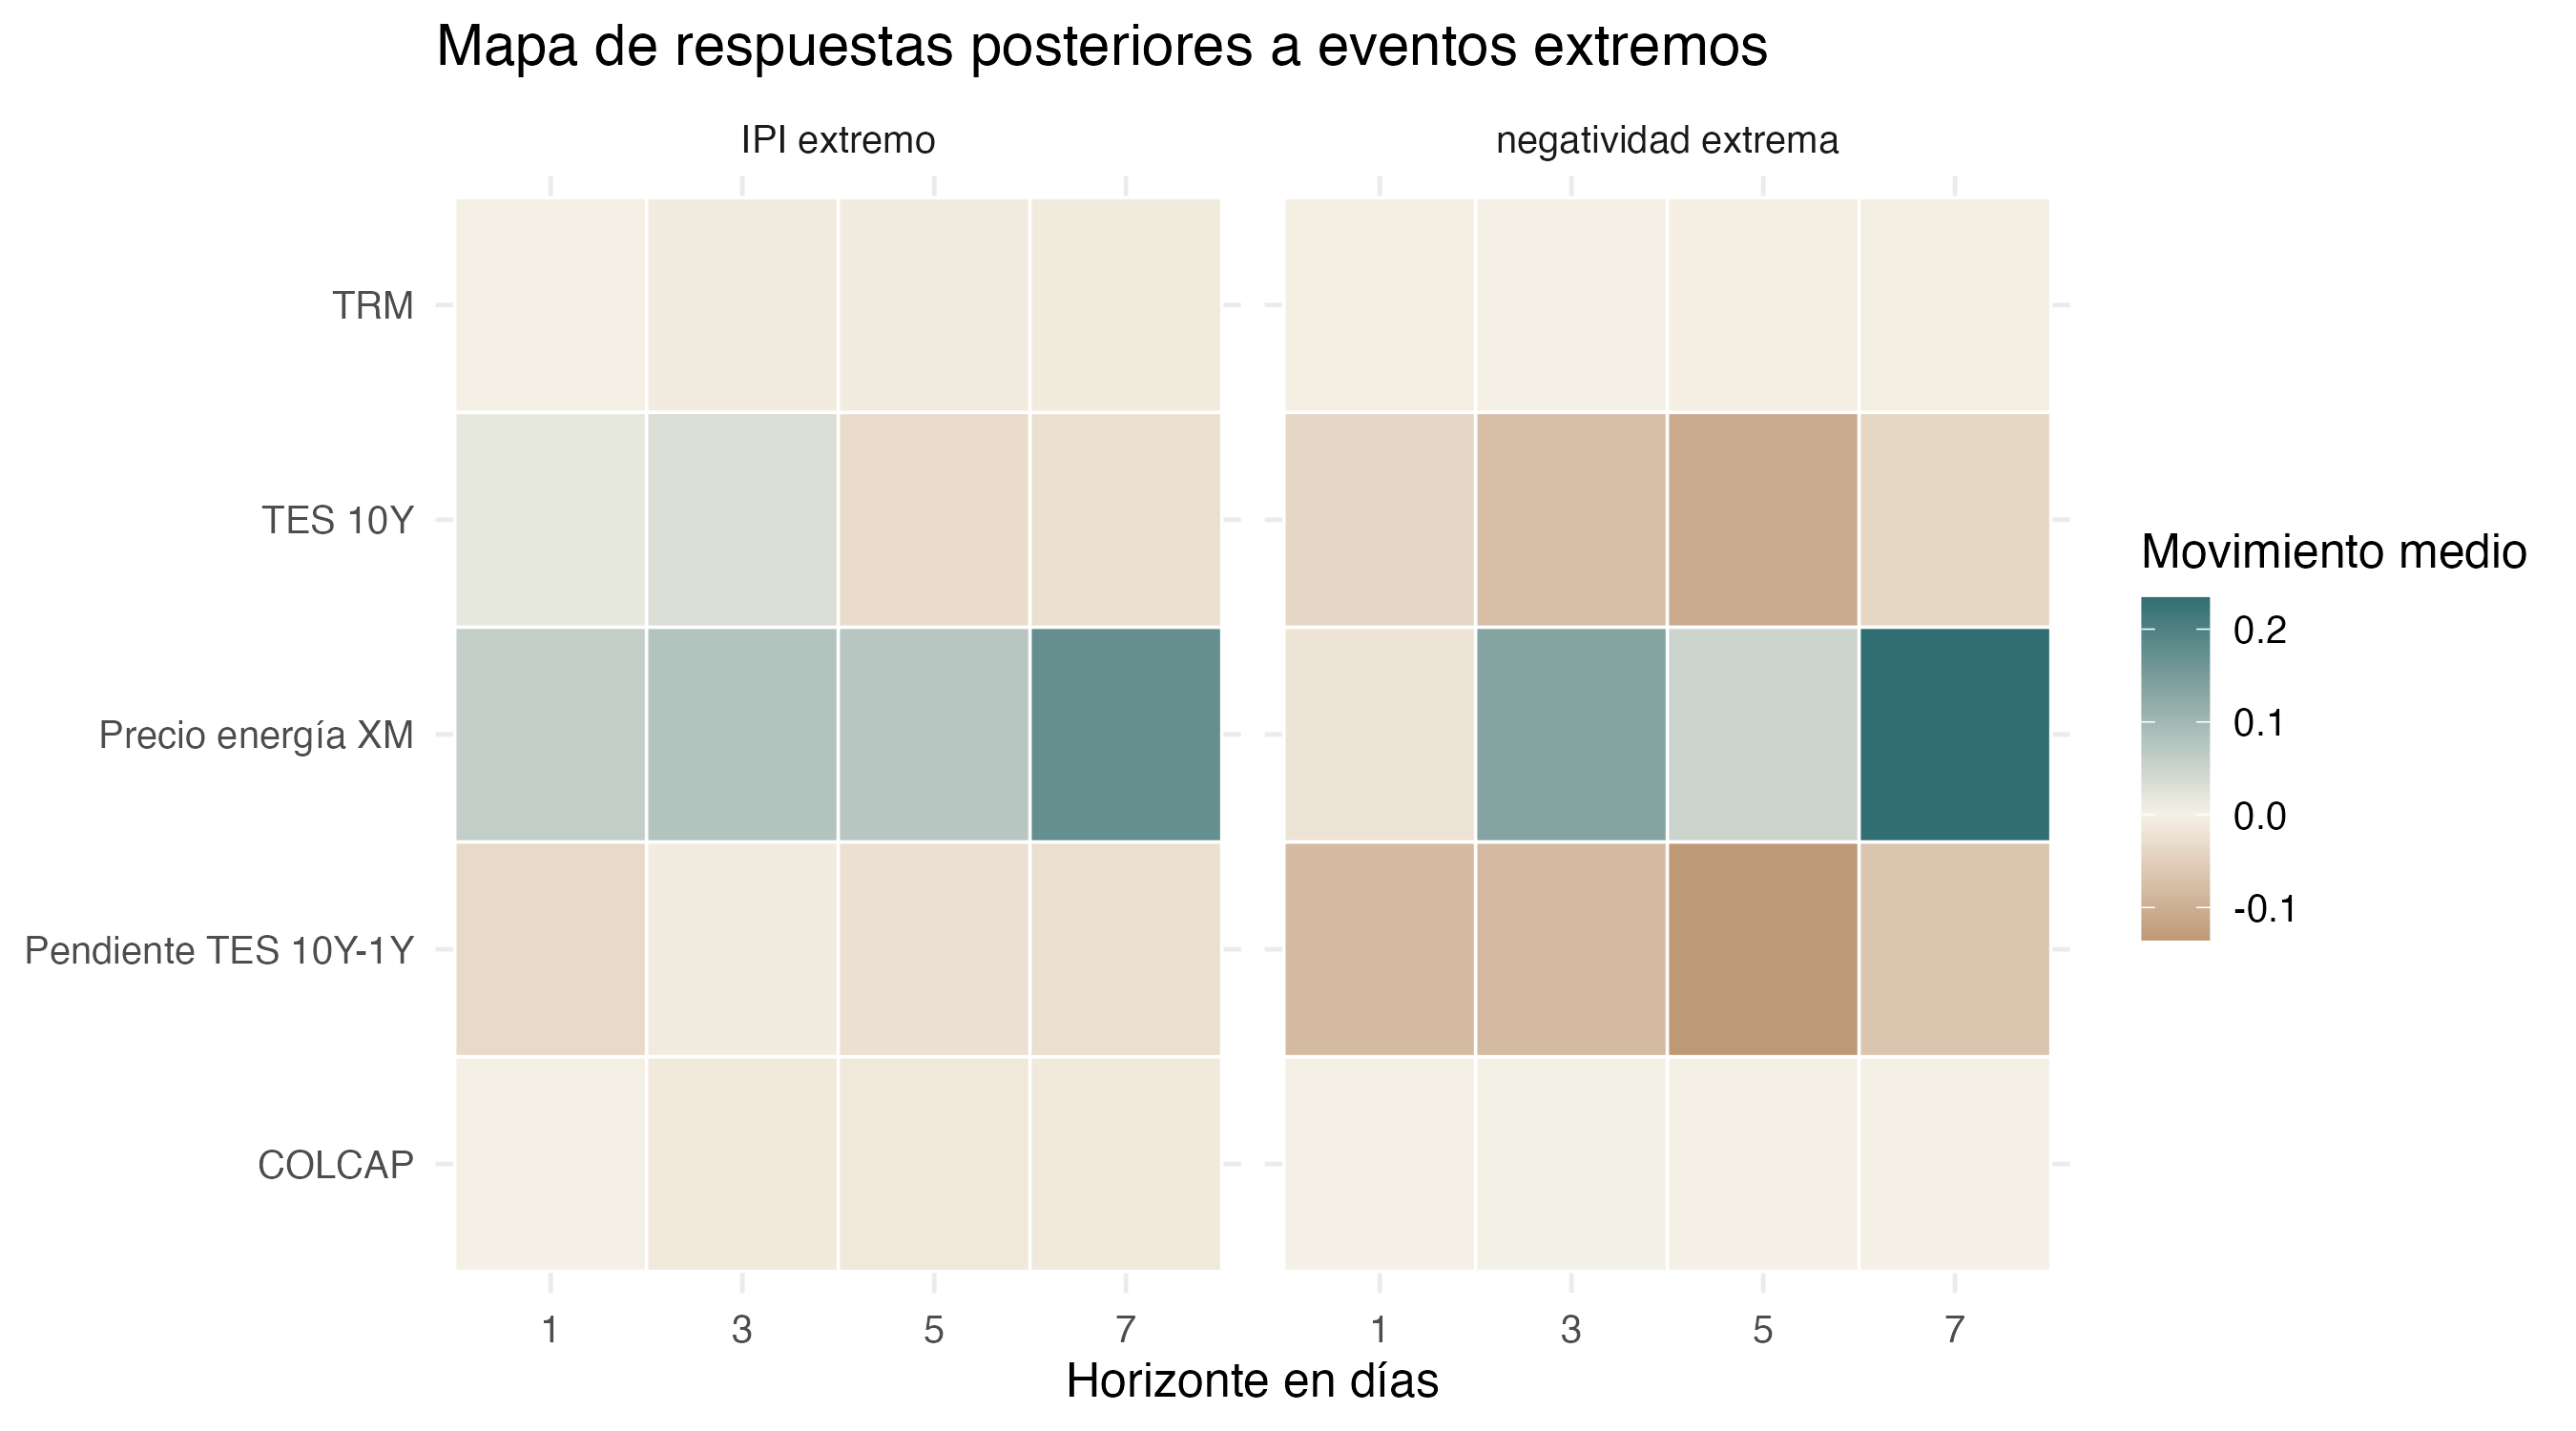
\includegraphics[width=0.9\linewidth,height=\textheight,keepaspectratio]{figures/event_study_respuestas_heatmap.png}

}

\caption{\label{fig-event-study-heatmap}Heatmap de respuestas promedio
por horizonte y serie financiera.}

\end{figure}%

\section{Discusión preliminar}\label{discusiuxf3n-preliminar}

La principal diferencia frente al paper original no es únicamente el
tamaño de la muestra, sino la separación conceptual entre reacción
social y emisión presidencial. En el ejercicio inicial, las consultas
sobre Petro podían mezclar voces de apoyo, crítica, prensa y mensajes
del propio presidente. La arquitectura actual hace visible esa
diferencia: el corpus \texttt{opinion} mide clima discursivo alrededor
de Petro, mientras que el corpus \texttt{presidente} mide intensidad y
contenido de una cuenta con poder institucional.

Las redes estilo \texttt{quanteda} ayudan a leer esa distinción sin
cambiar la lógica metodológica original. Hashtags y menciones no se
interpretan como pruebas aisladas de influencia, sino como mapas de
coaparición que muestran cómo se agrupan temas y actores. La frecuencia
de tweets presidenciales añade otra capa: meses con alta producción
comunicativa pueden amplificar la exposición pública de ciertas
discusiones, pero su efecto financiero depende del contexto, del
contenido y de la reacción social medida en el corpus \texttt{opinion}.

Por esa razón, los resultados econométricos deben mantenerse como
evidencia de precedencia y sincronía. La combinación de sentimiento,
volumen, IPI, Granger, VAR condicionado y estudio de eventos sugiere que
el discurso político puede contener señales informativas para TRM,
COLCAP y TES en algunos momentos, pero no identifica por sí sola un
mecanismo causal estructural. La contribución del paper es dejar un
sistema reproducible para seguir esa relación con mejores datos y
diseños futuros.

\section{Conclusiones}\label{conclusiones}

Twitter/X ha transformado la forma en que líderes políticos se comunican
con ciudadanos, opositores, periodistas e inversionistas. El paper
original sostenía que los mensajes de un presidente pueden influir en la
imagen colectiva de su administración y, eventualmente, reflejarse en el
mercado financiero. La versión actual fortalece y precisa ese argumento:
el corpus \texttt{opinion} evidencia una conversación polarizada,
emocionalmente intensa y estructurada por reformas, paz total y
expectativas económicas, mientras el corpus \texttt{presidente} permite
observar el discurso directo de \texttt{@petrogustavo} sin atribuirle
voces de terceros.

La evidencia textual es más rica que en el documento inicial. Las redes
de hashtags y menciones replican el estilo oficial de análisis de
Twitter de \texttt{quanteda} y muestran confrontación, centralidad de
actores y agrupamientos semánticos. El EDA de frecuencia de tweets
presidenciales muestra que la actividad de \texttt{@petrogustavo} se
concentra en episodios específicos, con un aumento importante desde
finales de 2025. Keyness, las nubes de palabras TF-IDF y la evolución
temporal muestran que las reformas no constituyen un único campo
semántico y que el vocabulario cambia por periodo y corpus. La
supervisión débil mejora la lectura de \texttt{otros} con cautela;
Wordfish y STM ayudan a resumir posiciones y tópicos. NRC, sentometrics
y spaCy profundizan la lectura de tono, actores y patrones lingüísticos.

La evidencia de mercado es más completa, pero debe mantenerse prudente.
La actualización reemplaza fuentes locales frágiles por BanRep para TRM,
COLCAP y TES, e incorpora la pendiente TES 10Y-1Y como indicador de
renta fija soberana. Los resultados de Granger por corpus, VAR
condicionado y estudio de eventos son útiles para describir precedencia,
sincronía y predicción exploratoria, no para afirmar causalidad final
entre discurso presidencial, conversación pública y mercado.

La recomendación principal es metodológica e institucional. La
comunicación de altos funcionarios debe estudiarse con cuidado porque
puede afectar expectativas en entornos polarizados. Al mismo tiempo, la
interpretación responsable exige fuentes auditables, procesamiento
textual transparente y cautela frente a afirmaciones causales. La
versión mejorada conserva la advertencia original sobre sensatez y
prudencia en redes sociales, y agrega una arquitectura reproducible que
puede extenderse a nuevas consultas, indicadores financieros y diseños
causales más fuertes.

\section{Disclosure of interest}\label{disclosure-of-interest}

In accordance with Taylor \& Francis policy and our ethical obligations
as researchers, we report that we do not receive financial funding that
may be affected by the research reported in the enclosed paper.

\section{Declaration of funding}\label{declaration-of-funding}

No funding was received.

\phantomsection\label{refs}
\begin{CSLReferences}{1}{0}
\bibitem[\citeproctext]{ref-sentometrics_jss}
Ardia, David, Keven Bluteau, Samuel Borms, and Kris Boudt. 2021. {``The
{R} Package Sentometrics to Compute, Aggregate, and Predict with Textual
Sentiment.''} \emph{Journal of Statistical Software} 99 (2): 1--40.
\url{https://doi.org/10.18637/jss.v099.i02}.

\bibitem[\citeproctext]{ref-banrep_colcap}
Banco de la República. 2026a. {``{COLCAP} Daily Series Metadata.''}
\url{https://www.banrep.gov.co/en/node/50428}.

\bibitem[\citeproctext]{ref-banrep_sdmx}
---------. 2026b. {``Documento Técnico Para Consumo de Servicios Web
{SDMX}.''}
\url{https://suameca.banrep.gov.co/archivos/webservices/documento_tecnico_ws_consumo_sdmx.pdf}.

\bibitem[\citeproctext]{ref-banrep_tes}
---------. 2026c. {``{TES} Zero-Coupon Interest-Rate Series Metadata.''}
\url{https://www.banrep.gov.co/en/node/50444}.

\bibitem[\citeproctext]{ref-bayod_2018}
Bayod, María Jesús R. 2018. {``{Big data}: Crisis y Nuevos
Planteamientos En Los Flujos de Comunicación de La Cuarta Revolución
Industrial.''} \emph{Area Abierta} 18 (2): 39.

\bibitem[\citeproctext]{ref-benoit_spacyr}
Benoit, Kenneth, and Akitaka Matsuo. 2023. \emph{Spacyr: Wrapper to the
spaCy NLP Library}. \url{https://spacyr.quanteda.io}.

\bibitem[\citeproctext]{ref-benoit_textual_2018}
Benoit, Kenneth, Paul Nulty, Pablo Barber, Kohei Watanabe, and Benjamin
Lauderdale. 2018. {``Quantitative Analysis of Textual Data.''}

\bibitem[\citeproctext]{ref-quanteda}
Benoit, Kenneth, Kohei Watanabe, Haiyan Wang, Paul Nulty, Adam Obeng,
Stefan Müller, and Akitaka Matsuo. 2018. {``Quanteda: An r Package for
the Quantitative Analysis of Textual Data.''} \emph{Journal of Open
Source Software} 3 (30): 774. \url{https://doi.org/10.21105/joss.00774}.

\bibitem[\citeproctext]{ref-blei_2009}
Blei, David. 2009. {``Topic Models.''} videolectures.net.
\url{http://videolectures.net/mlss09uk_blei_tm/}.

\bibitem[\citeproctext]{ref-blei_2003}
Blei, David M., Andrew Y. Ng, and Michael I. Jordan. 2003. {``Latent
Dirichlet Allocation.''} \emph{Journal of Machine Learning Research} 3
(Jan): 993--1022.

\bibitem[\citeproctext]{ref-bondi_scott_2010}
Bondi, Marina, and Mike Scott. 2010. \emph{Keyness in Texts}. Vol. 41.
John Benjamins Publishing.

\bibitem[\citeproctext]{ref-casallas_2020}
Casallas Felipe, Miguel Annyelo. 2020. {``An{á}lisis de Contenido Sobre
La Percepci{ó}n Pol{í}tica de Gustavo Petro e Iv{á}n Duque En La Red
Social Twitter.''} \{B.S.\} thesis, Universidad de La Sabana.

\bibitem[\citeproctext]{ref-cavanillas_2016}
Cavanillas, José María, Edward Curry, and Wolfgang Wahlster. 2016.
\emph{New Horizons for a Data-Driven Economy: A Roadmap for Usage and
Exploitation of Big Data in Europe}. Springer Nature.

\bibitem[\citeproctext]{ref-opinion_mining_financial_2022}
Chen, Chung-Chi, Hen-Hsen Huang, and Hsin-Hsi Chen, eds. 2022.
\emph{From Opinion Mining to Financial Argument Mining}. Springer
Nature.

\bibitem[\citeproctext]{ref-chen_duan_yang_2022}
Chen, Kaiping, Zening Duan, and Sijia Yang. 2022. {``Twitter as Research
Data: Tools, Costs, Skill Sets, and Lessons Learned.''} \emph{Politics
and the Life Sciences} 41 (1): 114--30.

\bibitem[\citeproctext]{ref-conte_2012}
Conte, Rosaria, Nigel Gilbert, Giulia Bonelli, Claudio Cioffi-Revilla,
Guillaume Deffuant, Janos Kertész, Vittorio Loreto, et al. 2012.
{``Manifesto of Computational Social Science.''} \emph{The European
Physical Journal Special Topics} 214: 325--46.

\bibitem[\citeproctext]{ref-cornejo_2022}
Cornejo, José Emiliano Palma. 2022. {``Populismo, Pandemia y Tweets: El
Caso de Donald Trump Analizado Mediante La Metodolog{í}a de an{á}lisis
de Sentimientos.''}

\bibitem[\citeproctext]{ref-original_petro_paper}
Echeverry, Juan José. 2023. {``Impacto Del Discurso de Gustavo Petro En
Variables Económicas Colombianas.''}

\bibitem[\citeproctext]{ref-el_hamdouchi_1986}
El-Hamdouchi, Abdelmoula, and Peter Willett. 1986. {``Hierarchic
Document Classification Using Ward's Clustering Method.''} In
\emph{Proceedings of the 9th Annual International ACM SIGIR Conference
on Research and Development in Information Retrieval}, 149--56.

\bibitem[\citeproctext]{ref-field_2012}
Field, Andy, Jeremy Miles, and Zoë Field. 2012. \emph{Discovering
Statistics Using r}. SAGE.

\bibitem[\citeproctext]{ref-gomez_torres_2018}
Gómez-Torres, Estevan, Roger Jaimes, Orlando Hidalgo, and Sergio
Luján-Mora. 2018. {``Influencia de Redes Sociales En El an{á}lisis de
Sentimiento Aplicado a La Situaci{ó}n Pol{í}tica En Ecuador.''}
\emph{Enfoque UTE} 9 (1): 67--78.

\bibitem[\citeproctext]{ref-hirschberg_manning_2015}
Hirschberg, Julia, and Christopher D. Manning. 2015. {``Advances in
Natural Language Processing.''} \emph{Science} 349 (6245): 261--66.

\bibitem[\citeproctext]{ref-husson_2016}
Husson, François, Sébastien Lê, and Jérôme Pagès. 2016. \emph{Analyse de
Donn{é}es Avec r}. Presses universitaires de Rennes.

\bibitem[\citeproctext]{ref-hvitfeldt_silge_2022}
Hvitfeldt, Emil, and Julia Silge. 2022. \emph{Supervised Machine
Learning for Text Analysis in r}. CRC Press.

\bibitem[\citeproctext]{ref-hyndman_fpp}
Hyndman, Rob J., and George Athanasopoulos. 2018. \emph{Forecasting:
Principles and Practice}. 2nd ed. OTexts.
\url{https://otexts.com/fpp2/}.

\bibitem[\citeproctext]{ref-ince_2017}
Ince, Jelani, Fabio Rojas, and Clayton A. Davis. 2017. {``The Social
Media Response to Black Lives Matter: How Twitter Users Interact with
Black Lives Matter Through Hashtag Use.''} \emph{Ethnic and Racial
Studies} 40 (11): 1814--30.

\bibitem[\citeproctext]{ref-jockers_2017}
Jockers, Matthew. 2017. \emph{Package {syuzhet}}.
\url{https://cran.r-project.org/web/packages/syuzhet}.

\bibitem[\citeproctext]{ref-kahneman_1979}
Kahneman, Daniel. 1979. {``Prospect Theory: An Analysis of Decisions
Under Risk.''} \emph{Econometrica} 47: 278.

\bibitem[\citeproctext]{ref-kearney_2019}
Kearney, Michael W. 2019. {``Rtweet: Collecting and Analyzing Twitter
Data.''} \emph{Journal of Open Source Software} 4 (42): 1829.

\bibitem[\citeproctext]{ref-kleiber_zeileis}
Kleiber, Christian, and Achim Zeileis. 2008. \emph{Applied Econometrics
with r}. New York: Springer.

\bibitem[\citeproctext]{ref-kolaczyk_csardi_2020}
Kolaczyk, Eric D., and Gábor Csárdi. 2020. \emph{Statistical Analysis of
Network Data with r}. Springer.

\bibitem[\citeproctext]{ref-kumar2014_text_mining}
Kumar, Lalit, and Parul Kalra Bhatia. 2014. {``A Survey of Text Mining
Techniques and Applications.''} \emph{Journal of Emerging Technologies
in Web Intelligence} 6 (2): 243--48.

\bibitem[\citeproctext]{ref-kwartler_2017}
Kwartler, Ted. 2017. \emph{Text Mining in Practice with r}. John Wiley
\& Sons.

\bibitem[\citeproctext]{ref-marin_diaz_2020}
Marin Diaz, Juan Pablo. 2020. \emph{Genero: Estimate Gender from Names
in Spanish and Portuguese}. \url{https://github.com/datasketch/genero}.

\bibitem[\citeproctext]{ref-medhat_2014}
Medhat, Walaa, Ahmed Hassan, and Hoda Korashy. 2014. {``Sentiment
Analysis Algorithms and Applications: A Survey.''} \emph{Ain Shams
Engineering Journal} 5 (4): 1093--113.

\bibitem[\citeproctext]{ref-misuraca_2020}
Misuraca, Michelangelo, Alessandro Forciniti, Germana Scepi, and Maria
Spano. 2020. {``Sentiment Analysis for Education with r: Packages,
Methods and Practical Applications.''}
\url{https://arxiv.org/abs/2005.12840}.

\bibitem[\citeproctext]{ref-mittal_goel_2012}
Mittal, Anshul, and Arpit Goel. 2012. {``Stock Prediction Using Twitter
Sentiment Analysis.''} \emph{Stanford University, CS229} 15: 2352.
\url{http://cs229.stanford.edu/proj2011/GoelMittal-StockMarketPredictionUsingTwitterSentimentAnalysis.pdf}.

\bibitem[\citeproctext]{ref-mohammad_turney_2013}
Mohammad, Saif M., and Peter D. Turney. 2013. {``Crowdsourcing a
Word--Emotion Association Lexicon.''} \emph{Computational Intelligence}
29 (3): 436--65.

\bibitem[\citeproctext]{ref-mohammad_turney_2010}
Mohammad, Saif, and Peter Turney. 2010. {``Emotions Evoked by Common
Words and Phrases: Using Mechanical Turk to Create an Emotion
Lexicon.''} In \emph{Proceedings of the NAACL HLT 2010 Workshop on
Computational Approaches to Analysis and Generation of Emotion in Text},
26--34.

\bibitem[\citeproctext]{ref-msci_colcap}
MSCI. 2026. {``{MSCI COLCAP} Indexes.''}
\url{https://www.msci.com/our-solutions/indexes/index-profiles/market-cap-weighted/msci-colcap-indexes}.

\bibitem[\citeproctext]{ref-mullainathan_thaler_2000}
Mullainathan, Sendhil, and Richard H. Thaler. 2000. {``Behavioral
Economics.''} Cambridge, MA: National Bureau of Economic Research.

\bibitem[\citeproctext]{ref-perez_llorente_2020}
Pérez Llorente, José Manuel. 2020. {``El Impacto de Los Tweets de Donald
j. Trump Sobre Los Mercados Financieros.''}

\bibitem[\citeproctext]{ref-plutchik_2003}
Plutchik, Robert. 2003. \emph{Emotions and Life: Perspectives from
Psychology, Biology, and Evolution}. American Psychological Association.

\bibitem[\citeproctext]{ref-prada_espinel_2018}
Prada Espinel, Óscar A. 2018. {``Comportamiento Comunicacional de
Twitter En Las Campa{ñ}as Presidenciales de Colombia 2018: Caso Gustavo
Petro e Iv{á}n Duque.''} Master's thesis, Universidad Internacional de
Andaluc{í}a.

\bibitem[\citeproctext]{ref-quanteda_twitter_example}
quanteda team. 2026. {``Example: Social Media Analysis (Twitter).''}
\url{https://quanteda.io/articles/pkgdown/examples/twitter.html}.

\bibitem[\citeproctext]{ref-stm}
Roberts, Margaret E., Brandon M. Stewart, and Dustin Tingley. 2019.
{``Stm: An r Package for Structural Topic Models.''} \emph{Journal of
Statistical Software} 91 (2): 1--40.
\url{https://doi.org/10.18637/jss.v091.i02}.

\bibitem[\citeproctext]{ref-romero_moreno_2020}
Romero Moreno, Fanny Y., Carlos A. Sanchez Martelo, Bibiana Y. Alfonso
Corredor, Juan F. Sanchez Cifuentes, and Juan P. Ospina López. 2020.
{``An{á}lisis de Sentimiento a Las Opiniones Generadas En La Red Social
Twitter: Marketing Pol{í}tico.''}

\bibitem[\citeproctext]{ref-sandoval_marin_2022}
Sandoval Garrido, Luis E., and Mauricio Marín Jaramillo. 2022.
{``Elecciones Presidenciales y Desarrollo Municipal: El Caso Colombiano
(1986-2014).''} \emph{Revista Lecturas de Econom{í}a}, no. 97: 113--48.

\bibitem[\citeproctext]{ref-schweinberger_2023}
Schweinberger, Martin. 2023. \emph{Analyzing Co-Occurrences and
Collocations in r}. Brisbane. \url{https://ladal.edu.au/coll.html}.

\bibitem[\citeproctext]{ref-silge_robinson_2017}
Silge, Julia, and David Robinson. 2017. \emph{Text Mining with r: A Tidy
Approach}. O'Reilly Media.

\bibitem[\citeproctext]{ref-slapin_proksch_2008}
Slapin, Jonathan B., and Sven-Oliver Proksch. 2008. {``A Scaling Model
for Estimating Time-Series Party Positions from Texts.''} \emph{American
Journal of Political Science} 52 (3): 705--22.

\bibitem[\citeproctext]{ref-smith_1759}
Smith, Adam. 1759. \emph{The Theory of Moral Sentiments}. London;
Edinburgh: Printed for A. Millar; A. Kincaid; J. Bell.

\bibitem[\citeproctext]{ref-stefanowitsch_gries_2003}
Stefanowitsch, Anatol, and Stefan Gries. 2003. {``Collostructions:
Investigating the Interaction of Words and Constructions.''}
\emph{International Journal of Corpus Linguistics} 8.
\url{https://doi.org/10.1075/ijcl.8.2.03ste}.

\bibitem[\citeproctext]{ref-stefanowitsch_gries_2005}
---------. 2005. {``Covarying Collexemes.''} \emph{Corpus Linguistics
and Linguistic Theory} 1: 1--43.
\url{https://doi.org/10.1515/cllt.2005.1.1.1}.

\bibitem[\citeproctext]{ref-steinert_threlkeld_2018}
Steinert-Threlkeld, Zachary C. 2018. \emph{Twitter as Data}. Cambridge
University Press.

\bibitem[\citeproctext]{ref-trott_2018}
Trott, Verity. 2018. {``Connected Feminists: Foregrounding the
Interpersonal in Connective Action.''} \emph{Australian Journal of
Political Science} 53 (1): 116--29.

\bibitem[\citeproctext]{ref-urdinez_cruz_2020}
Urdinez, Francisco, and Andrés Cruz. 2020. \emph{R for Political Data
Science: A Practical Guide}. CRC Press.

\bibitem[\citeproctext]{ref-wiedemann_niekler_2017}
Wiedemann, Gregor, and Andreas Niekler. 2017. {``Hands-on: A Five Day
Text Mining Course for Humanists and Social Scientists in r.''} In
\emph{Proceedings of the Workshop on Teaching NLP for Digital Humanities
(Teach4DH@GSCL 2017)}, 57--65.
\url{http://ceur-ws.org/Vol-1918/wiedemann.pdf}.

\end{CSLReferences}




\end{document}
